\documentclass[12pt, a4paper]{article}
\usepackage[paper=a4paper, left=1.5cm, right=1.5cm, bottom=2cm, 		top=2cm]{geometry}
\usepackage[utf8]{inputenc}
\usepackage[T1]{fontenc}
%\usepackage[spanish]{babel}
\usepackage{aed2-symb,aed2-itef,aed2-tad,aed2-tokenizer}
\usepackage{newalgo}
\usepackage{interfaz}
\usepackage{caratula}
\newcommand{\comment}[1]{}
\usepackage{verbatim}
\usepackage{algorithm}
\usepackage{algpseudocode}
\usepackage{algorithmicx}
\usepackage{graphicx}
\usepackage[colorlinks,citecolor=black,filecolor=black,linkcolor=black,    urlcolor=black]{hyperref}
\setcounter{secnumdepth}{5}
\setcounter{tocdepth}{5}
\let\state\State
\let\while\While
\let\endwhile\EndWhile
%\let\if\If
\let\endif\EndIf
%\let\else\Else
%\let\elseif\ElsIf


\titulo{Trabajo Pr\'actico 3}
\materia{Algoritmos y Estructura de Datos III}
\grupo{ }
\integrante{Candioti, Alejandro}{784/13}{amcandio@gmail.com}
\integrante{Maldonado, Kevin}{018/14}{maldonadokevin11@gmail.com}
\integrante{Tripodi, Guido}{843/10}{guido.tripodi@hotmail.com}


\begin{document}

\maketitle
\tableofcontents
\newpage

\newpage
\section{Ejercicio 1} 
\subsection{Enunciado del problema}
En este punto y en los restantes contaremos con un personaje llamado Indiana Jones, el cual buscara resolver la pregunta mas importante de la computacion, es P=NP?.\\

Focalizandonos en este ejercicio, Indiana, ira en busca de una civilizacion antigua con su grupo de arqueologos, ademas, una tribu local, los ayudara a encontrar dicha civilizacion, donde se encontrara con una dificultad, la cual sera cruzar un puente donde el mismo no se encuentra en las mejores condiciones.\\

Para cruzar dicho puente Indiana y el grupo cuenta con una unica linterna y ademas, dicha tribu suele ser conocida por su canibalismo, por lo tanto al cruzar dicho puente no podran quedar mas canibales que arqueologos.

Nuestra intencion sera ayudarlo a cruzar de una forma eficiente donde cruze de la forma mas rapido todo el grupo sin perder integrantes en el intento.

Por lo tanto, en este ejercicio nuestra entrada seran la cantidad de arqueologos y canibales y sus respectivas velocidades.


\subsection{Explicaci\'on de resoluci\'on del problema}
El enunciado presenta el problema de hallar el camino entre 2 puntos que se recorra en el menor tiempo posible, dandonos un escenario en donde los caminos presentan paredes que podemos atravezar rompiendolas, teniendo a la vez, una determinada cantidad de rupturas a poder realizar. La solución buscada será entre todos los caminos posibles desde el origen al destino, el que sea mínimo.

Cada camino esta compuesto de unas unidades "caminables", que las llamaremos baldozas. Ir de una baldoza a otra consume la misma cantidad de tiempo en todos los casos. Por otro lado, hay 
baldozas que demandan romper una pared para ser caminadas, con lo cual el camino que se esta transitando debe gastar 1 unidad de esfuerzo en romperla, factor que no influye en el tiempo del recorrido.

Si caracterizamos cada baldoza con un nodo, y la posibilidad de ir de una baldoza a otra como una arista, entonces podemos modelar el problema con un grafo. Como el factor tiempo es constante en cada traslado entre baldozas, las aristas tendrán todas el mismo peso.

A partir de este grafo, sacar el camino mínimo del nodo origen al destino se puede realizar utilizando el algoritmo de busqueda por anchura, el cual permite saber la distancia (o tiempo) a la que se encuentran de determinado nodo cada uno de los demas. De aplicarlo sobre la estructura propuesta en forma directa, se obtendrían soluciones invalidálidas, ya que es necesario tener en cuenta la restricción de cantidad de paredes para romper. También se puede ver que el algoritmo solo, no considera todos los posidbles caminos válidos hacia el destino, con lo que se pierden soluciones validas, al restringir el uso de cada nodo a 1 solo camino:

  \vspace*{0.3cm} \vspace*{0.3cm}
  \begin{center}
 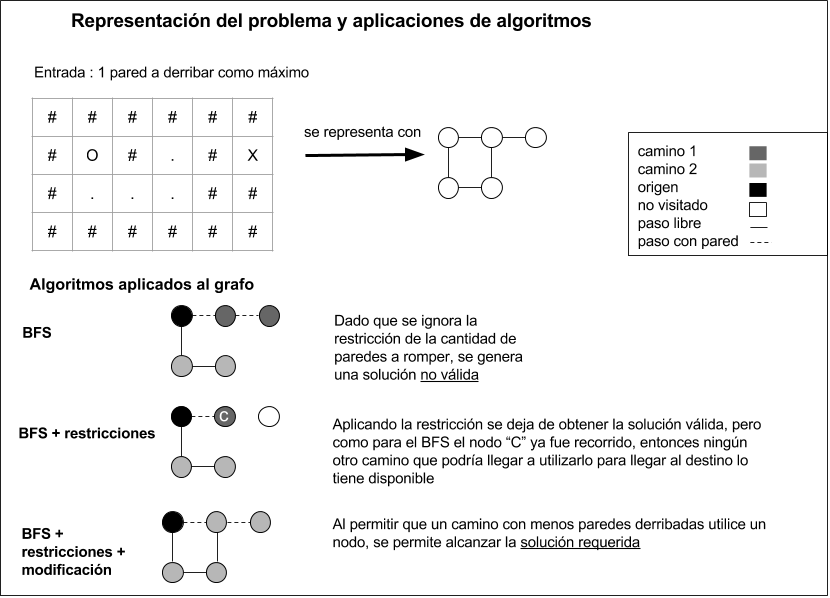
\includegraphics[scale=0.6]{./EJ1/ej1-explicacion.png}
  \end{center}
  \vspace*{0.3cm}

Para poder calcular todos los caminos que pueden llegar efectivamente al destino, en cada nodo se guardará las caracteristicas de tiempo y paredes necesarias para alcanzarlo:
\begin{itemize}
\item Si no ha sido alcanzado, entonces, se guarda el estado en el que se encuentra el nodo desde donde hacemos la visita: si se atravezo una o más paredes para lograrlo, se marca en su estado, al igual que el tiempo insumido en alcanzarlo.
\item Si ya ha sido alcanzado, entonces si la cantidad de paredes rotas hasta llegar hasta él por el camino actual es menor a la cantidad de paredes que fueron rotas anteriormente, entonce se considera que el camino actual es la mejor forma de alcanzar al nuevo nodo, guardando los datos del camino actual en el nodo.
\item En el caso de que alcanzar al nodo previamente visitado, demande el mismo tiempo y esfuerzo que en el camino actual, se desestima el camino actual.
\item Si el nodo a evaluar es el destino, se da por finalizado el algoritmo y se devuelve el estado del camino que lo alcanzó.
\end{itemize}

\newpage
\section{Ejercicio 2} 
\subsection{Enunciado del problema}
Una vez que el equipo fue avanzando por el laberinto en b\'usqueda de la X, se fueron encontrando con piezas de una tabla en el suelo, las cuales ten\'ian un manuscrito antiguo. Por lo tanto, quisieron juntar todas las piezas que compoñ\'ian la tabla. Similar al punto anterior, encontraremos el camino posible realizando el menor esfuerzo para recorrer todas las salas y juntar las piezas para armar la tabla completa.\\



\subsection{Explicaci\'on de resoluci\'on del problema}
En esta ocasión se debe encontrar, dada una serie de habitaciones, la forma menos costosa de unirlas, teniendo que derribar determinadas paredes para lograrlo. Dada 2 habitaciones: el muro menos costoso para derribar que las une será la elección a tomar para formar la solución, es decir, se deben elegir todos los muros menos costosos que unen las distintas habitaciones para obtener la solucion buscada.

Un planteo de modelo sobre grafo caracteriza a cada habitación como un conjunto de puntos caminables y cada uno de estos como un nodo adyacente a los puntos de la misma habitacion, el cual posee H componentes conexas, siendo H la cantidad total de habitaciones en el mapa. Lo que se busca entonces es una forma de unir estas componentes de la forma menos costosa. Para ello las unimos a 2 habitaciones separadas por una pared con un eje de peso igual al esfuerzo de derribarla. A las aristas de las componentes les asignamos el peso nulo.

CLAVAR EL DRAWING

Para obtener la solucion, se busca el AGM del grafo planteado mediante el algoritmo de Kruskal; a él se le calcula el peso, el cual representa la respuesta al problema.


\subsection{An\'alisis de complejidades}

Nuestro algoritmo como mencionamos anteriormente presenta 3 etapas.\\
La primera de ellas consta en recorrer desde $3^0$ hasta $3^i$ donde este ultimo sea igual a $P$ o en su defecto el inmediato mayor. Por lo tanto mostraremos que recorrer hasta un i donde $3^i$ sea igual o inmediatamente mayor a P es menor o igual a $\sqrt{P}$.\\


Si $i = 0$ $\Rightarrow$ terminamos.\\
Luego sea $3^i \geq P \geq 3^{i-1}$ con $i > 0$. Queremos ver que $i \leq \sqrt{P}$:\\
Se que por definici\'on $P \geq 3^{i-1}$ $\Rightarrow$ $\sqrt{P} \geq \sqrt{3^{i-1}}$\\
Veamos que $\sqrt{3^{i-1}} \geq i \Rightarrow 3^{i-1} \geq {i^2}$. Para $i = 1$ tenemos que $3^{1-1} \geq 1$ siempre. Luego, para $i > 1$ como ${3^{i-1}}$ es creciente y mayor o igual que $i^2$ se cumple siempre esta desigualdad. Por lo tanto queda probado que recorrer hasta un i tal que $3^i \geq P$ se encuentra en el orden de  O($\sqrt{P}$).\\


 Luego, creamos dos enteros \textit{saldoEnBalanza} y \textit{N} y un array \textit{arrayPesasUtilizadas} inicializado vacio, por lo tanto, como son enteros y el array es vacio esto insume O(1), finalizando as\'i la primera etapa.\\
Luego, la segunda etapa y m\'as importante de nuestro algoritmo, consiste en un ciclo donde realizaremos iterativamente la busqueda de las pesas que, sumando sus valores, nos de el valor $P$. Dicho ciclo en el peor de los casos recorrer\'a desde el valor de i que conten\'ia la pesa de mayor valor hasta i = 0, lo cual ser\'a O($\sqrt{P}$) ya que al trabajar con potencias de 3 la cantidad de vueltas del ciclo entraran en el orden de $\sqrt{P}$ como hab\'iamos demostrado anteriormente.\\ 

Dentro de este ciclo, realizamos 6 comparaciones en O(1) las cuales son:

\begin{itemize}
\item si N=0, si N=1, aqu\'i agregamos el valor de la pesa al array y terminamos el ciclo, esto insumir\'a O(1)
 \item si N es menor al valor de \textit{saldoEnBalanza}, estas opcion no finaliza el ciclo,
 agrega la pesa n el array, modifica el valor de saldoEnBalanza por el valor de N y disminuye en 1 a i, luego se chequea aqui mismo si $N < 0$ de ser verdadero se modifica el valor de $estaEnNegativo$ por verdadero o por falso en caso de ser falsa la guarda, lo cual insumir\'a O(1) cada una de las operaciones mencionadas, luego se chequea aqui mismo si $N < 0$ de ser verdadero se modifica el valor de $estaEnNegativo$ por verdadero o por falso en caso de ser falsa la guarda
 \item por ultimo, si $N \geq saldoEnBalanza$ solamente descontamos en uno a i para continuar con el ciclo.
\end{itemize} 
Una vez finalizado esto y por consiguiente la segunda etapa, pasamos a la tercera la cual consiste en guardar en \textit{arrayI} o \textit{arrayD} los valores de los elementos del \textit{arrayPesasUtilizadas} para colocarlos en la balanza del lado derecho o del izquierdo.\\
Para realizar esto recorremos el array \textit{arrayPesasUtilizadas} el cual en el peor de los casos tendr\'a todas las pesas, lo cual como vimoss recorrer la totalidad de elementos del array se encuentra en el orden de O($\sqrt{P}$).\\

Luego de ver esto, dentro del ciclo realizamos operaciones en O(1).\\
Por ultimo, devolvemos los array invirtiendo las posiciones de los elementos lo que insumir\'a en el peor de los caso O($\sqrt{P}$).\\

En conclusi\'on nuestro algoritmo realiza 4 ciclos que demandan en el peor de los casos O($\sqrt{P}$) donde dentro de los mismos se realizan operaciones en O(1), por lo tanto nuestra complejidad final ser\'a
O($\sqrt{P}$).





%\subsection{Experimientos y conclusiones}
%\subsubsection[2.5]{Test}
%\indent En los siguientes tests queremos observar que sucede con cada familia de casos al ir variando los parámetros de entrada F, C de manera creciente y lineal y tomando los tiempos de corrida de cada input para poder compararlos.\\
Se comienza, por lo tanto, con una entrada de F*C = N y se la hace crecer en $n$ filas y columnas en cada instancia, por lo tanto cada familia crece linealmente. De manera que no hay desigualdades y todas las familias se miden en instancias de igual tamaño e igual cantidad de paredes.\\

Para obtener dichas instancias se realizaron aproximadamente unas 20 corridas con el mismo input y se tom\'o el promedio de esas 20 corridas en cada instancia para obtener un valor m\'as cercano a la media.\\ 

\textit{---> 20 corridas ? no fueron mas?!!! PREGUNTA SERIA: LOS PARAMETROS AUMETAN LINEALMENTE EN LOS TESTS? ESO ES RE IMPORTANTE SI QUEREMOS ALGO CON UNA MEJOR FORMA}\\

Se pueden observar en el  gráfico 2.1, cinco funciones, que representan el tiempo de ejecuci\'on de las familias de casos mencionadas en el apartado anterior:\\

\begin{enumerate}
\item No existe arbol que conecte todas las salas
\item Existe un camino que conecta todas las salas de esfuerzo 0
\item El AGM es todo el grafo
\item Sin ejes
\item Camino por las salas random
\end{enumerate}

\vspace*{0.3cm} \vspace*{0.3cm}
  \begin{center}
 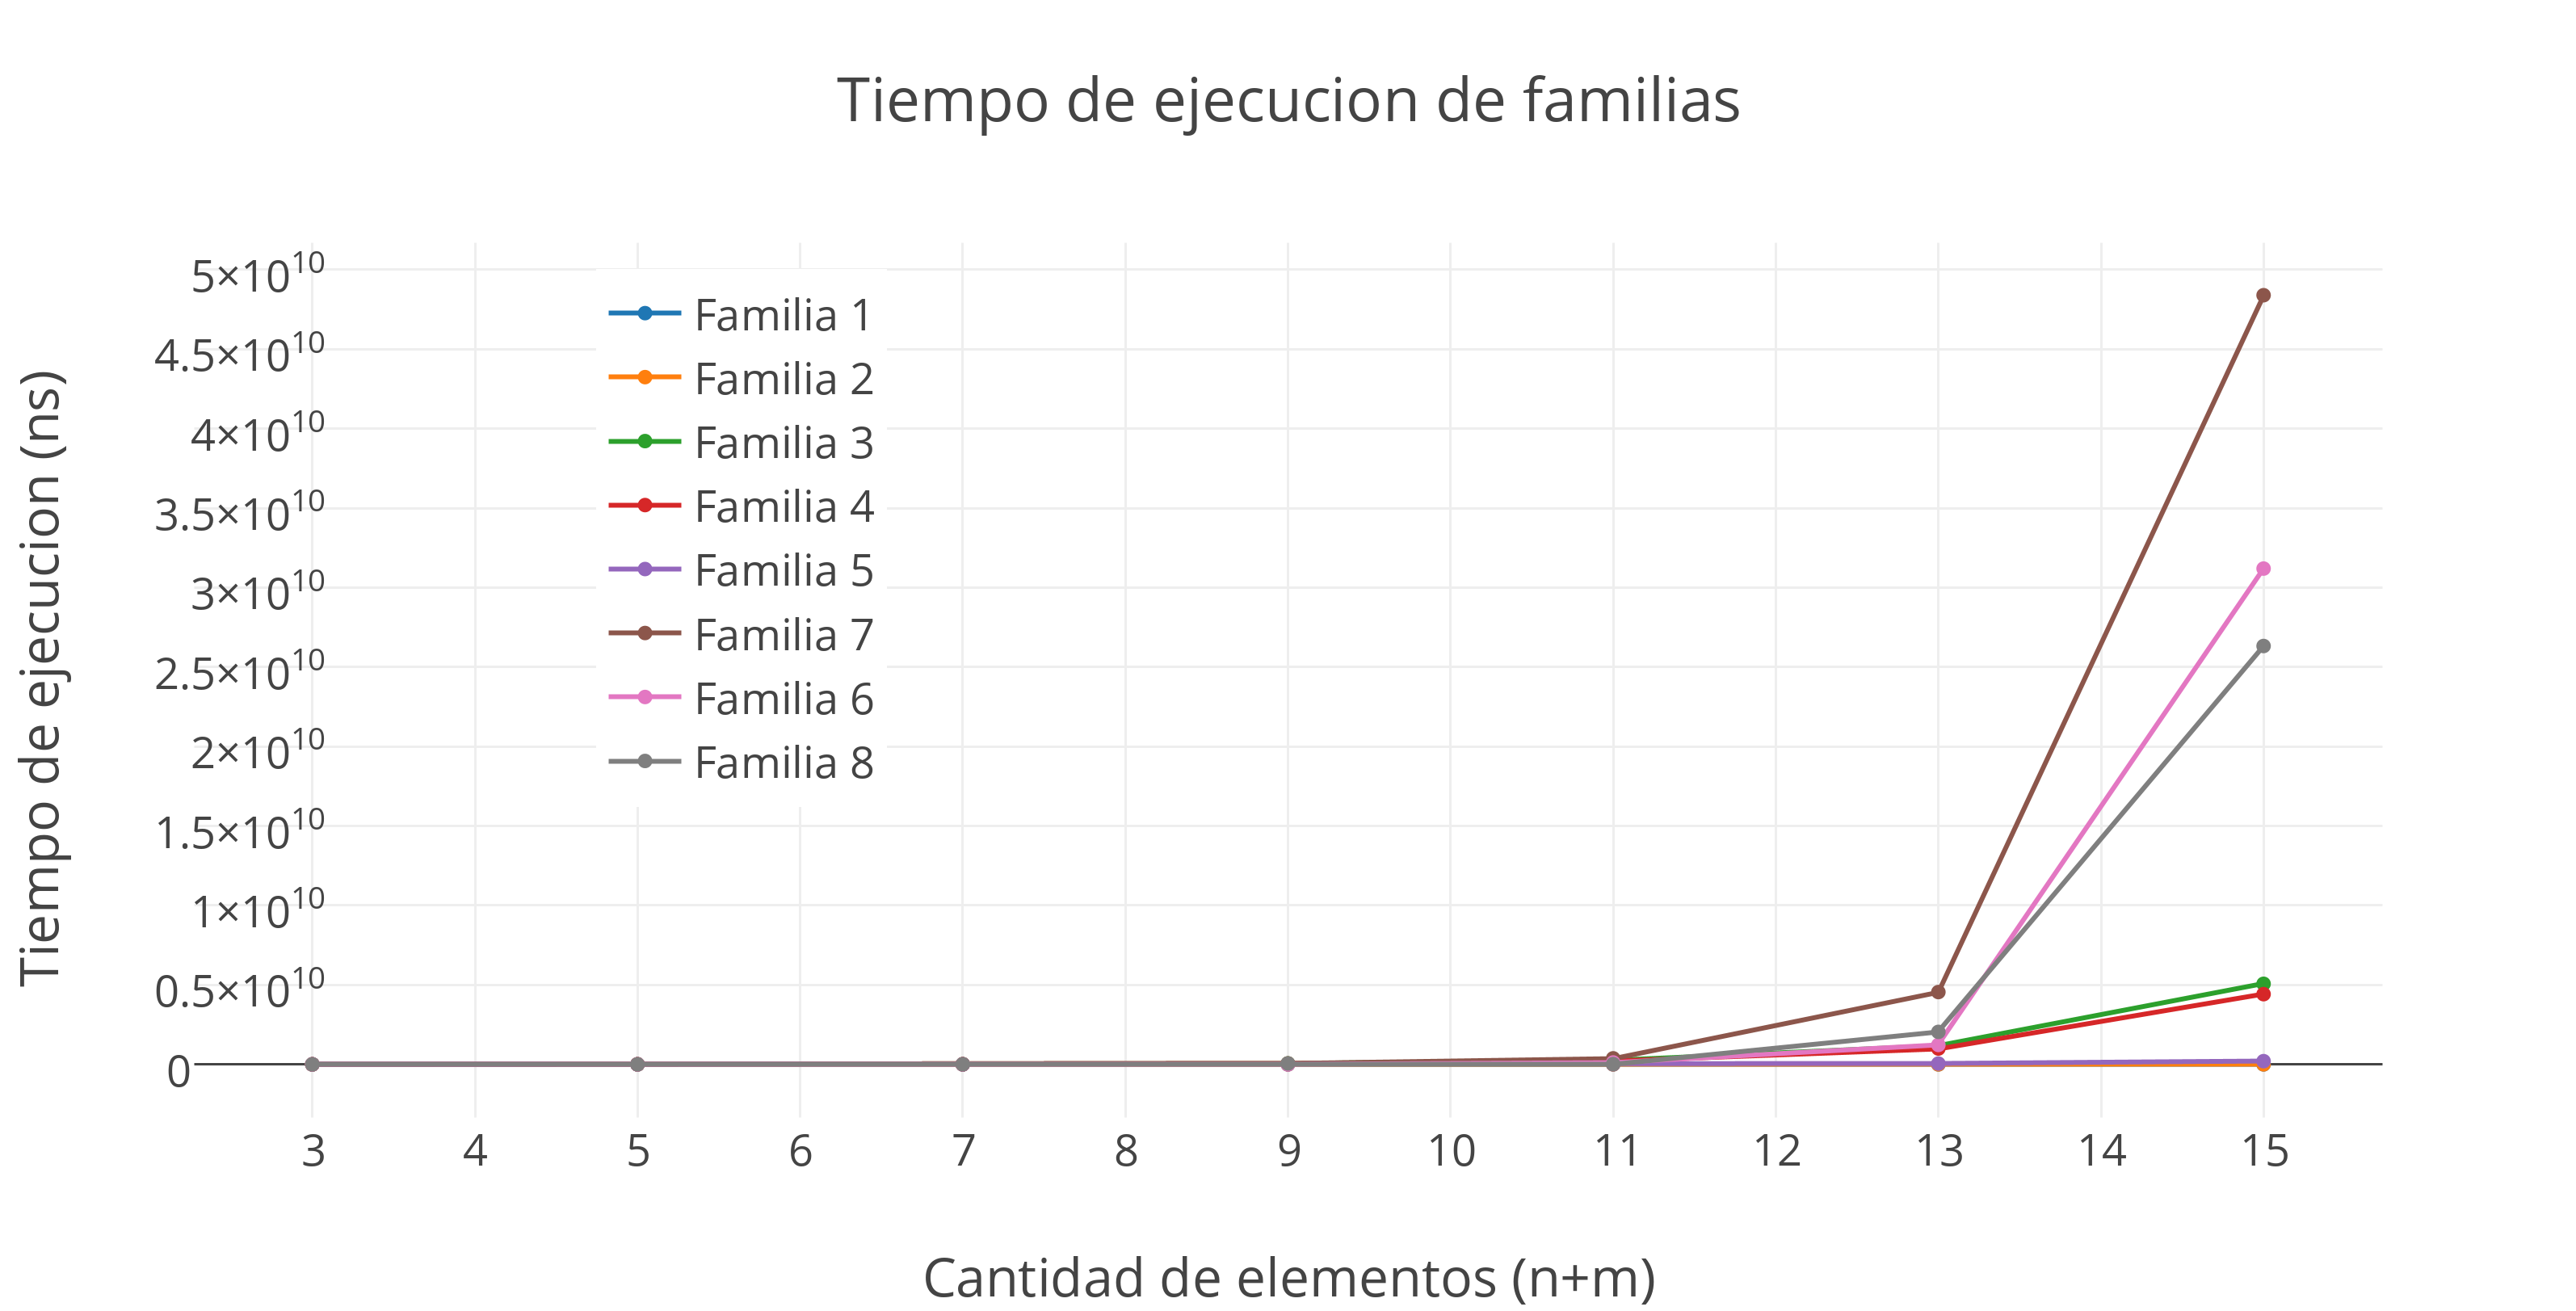
\includegraphics[scale=0.65]{./EJ2/comparativo.png}
 {$Gr$\'a$fico$ \ 2.1 - $Comparativo$}
  \end{center}
  \vspace*{0.3cm}
 
\textit{---> VER GRAFICO: REHACER. OJO LAS ETIQUETAS DEL GRAFICO, LA COMPLEJIDAD NO IRIA}\\

Como se observa en el gr\'afico la funci\'on representativa de la familia 4, presenta una mejor performance en relaci\'on a las otras. Esto se debe a que nuestro algoritmo al intentar chequear las aristas, observa que no hay ninguna y finaliza su ejecuci\'on insumiendo en tiempo unicamente la creaci\'on del grafo (nodos aislados)

Habiendo chequeado dichas instancias, llegamos a la conclusi\'on que la familia de casos que presenta una mejor performance para nuestro algoritmo
es la número 4 "\textbf{No existe arbol que conecte todas las salas}" dado que el grafo que se obtiene de transformar el laberinto recibido como par\'ametro no presenta ninguna arista.\\

Un grafo representativo de esta familia ser\'ia el siguiente:

\vspace*{0.3cm} \vspace*{0.3cm}
  \begin{center}
 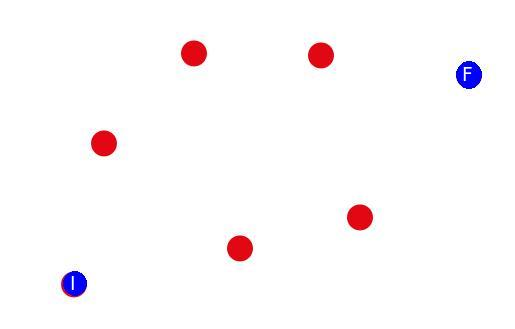
\includegraphics[scale=0.5]{./EJ2/grafoSinEjes.jpeg}
 \\{$Grafo$ \ 2.1 - $Mejor$ $Caso$}
  \end{center}
  \vspace*{0.3cm}

Verificando el peor caso en el gráfico 2.1, llegamos a la conclusi\'on que la familia de casos que hace que el algoritmo tenga más tiempo de computo ser\'a la familia 2 "\textbf{Existe un camino que conecta todas las salas de esfuerzo 0}" dado que el grafo que se obtiene de transformar el laberinto de entrada es aquel que presenta un ciclo por cada habitaci\'on posible, dandonos el siguiente grafo una vez transformado:\\

\vspace*{0.3cm} \vspace*{0.3cm}
  \begin{center}
 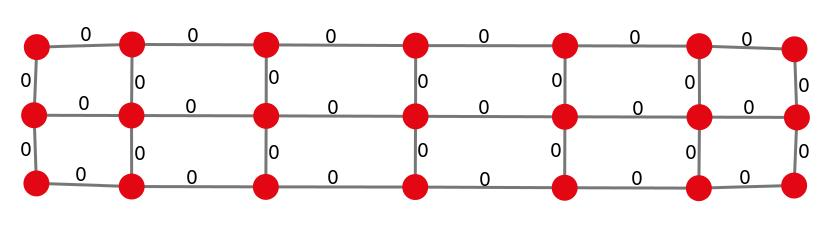
\includegraphics[scale=0.5]{./EJ2/ej2grafosinpared.jpeg}
 \\{$Grafo$ \ 2.2 - $Peor$ $Caso$}
  \end{center}
  \vspace*{0.3cm}
  
\textit{---> habria que explicar un poco que pasa en los otros casos!!!}\\
  
Veamos en detalle como se comportan el mejor y peor caso con respecto a la complejidad teorica calculada.\\

\vspace*{0.3cm} \vspace*{0.3cm}
  \begin{center}
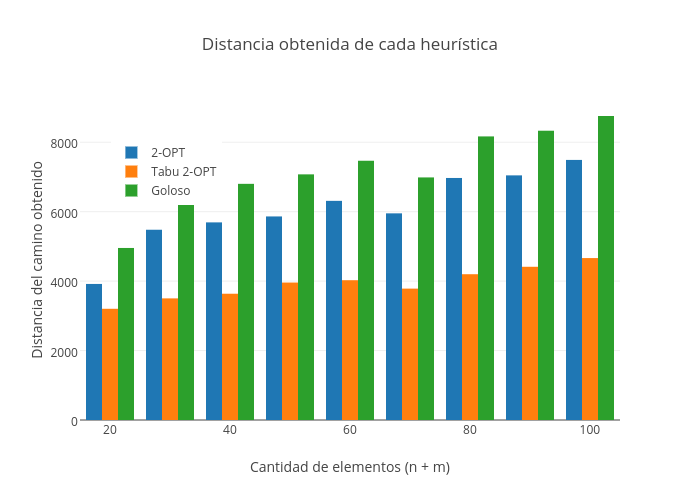
\includegraphics[scale=0.65]{./EJ2/comparativo1.png}
 {$Gr$\'a$fico$ \ 2.5 - $Comparativo$}
  \end{center}
  \vspace*{0.3cm}
  
\textit{---> VER GRAFICO: ESTE NO ES EL COMPARATIVO DE MEJOR Y PEOR. OJO LAS ETIQUETAS DEL GRAFICO, LA COMPLEJIDAD LA FITEAMOS}\\  
  
Podemos ver en este gr\'afico comparativo como las familias est\'an acotadas por la funci\'on de la complejidad te\'orica calculada.\\

\textit{---> Cuando retestiemos, vamos a fitear esto con nuestra complejidad, que no se como es, luego tenemos que hacer alguna conclusion. Deberia ser algo cuadratica.}\\
  
Luego de dichos experimentos y casos probados, se puede concluir que a pesar de tener ciclos en todas las salas y donde dichos ciclos presenten aristas con pesos iguales lo que genera al algoritmo la posibilidad de crear varias ramas posibles de soluci\'on los tiempos se mantienen dentro de la complejidad propuesta.\\



\newpage
\section{Ejercicio 3} 
\subsection{Enunciado del problema}
Luego de haber conseguido todas las piezas, llegan a la cruz y se encuentran con unos carritos apoyados sobre unas v\'ias las cuales al parecer llegan hasta afuera de la fortaleza. De un momento a otro, el equipo empieza a escuchar ruidos de adentro del laberinto, de tanto romper las paredes, la estructura se estaba desplomando, es por esto que deben conseguir un escape r\'apido, como al lado del carrito ven que se encuentra un mapa con estaciones y el final, nos solicitan ayuda para encontrar el camino m\'inimo de estaciones para llegar afuera de la forma m\'as r\'apida y eficiente.
\subsection{Explicaci\'on de resoluci\'on del problema}
%La soluci\'on planteada utiliza la t\'ecnica algor\'itmica de \textit{backtracking}. La idea es %recorrer todas las configuraciones posibles manteniendo la mejor soluci\'on encontrada hasta el momento. 

%Inicialmente, ordenaremos en base al peso y el valor de todos los objetos.\\
%Luego de realizar esto iremos agregando en las mochilas los objetos de mayor valor teniendo en cuenta el peso de los mismos con la mochila, en caso de que al agregar un objeto la suma de los pesos de los objetos que se encuentran en la mochila diera igual o mayor al peso m\'aximo de la mochila, se quitar\'a el objeto ultimo y se probar\'a con otro objeto de menor peso.\\
%As\'i realizaremos todas las posibles permutaciones de objetos en la mochila.\\
%Una vez que obtuvimos todas las permutaciones posibles nos quedaremos con la m\'axima, de esta manera tendr\'iamos en las mochilas una cantidad \'ptima de objetos con el mayor valor posible y un peso acorde a lo soportado por las mochilas.\\


%Las solucion planteada se basa en una generalización del problema de la mochila extendida a las 3 mochilas indicadas en la cota dada por la consigna.\\
\subsubsection*{Obteniendo el valor máximo}
 El problema de la mochila analiza, para cada objeto, el máximo valor que se puede obtener para cada capacidad posible de la mochila.Si llamamos K a la capacidad de la mochila, se evaluara introducir   el elemento suponiendo capacidad $k_{i}$ para i = 1, 2,..., hasta K. En cada evaluación se decide entre no meter el elemento, con lo cual el valor máximo de la mochila que tenga la capacidad $k_{i}$ será el calculado con algun elemento anterior (o cero en el caso de que sea el primero en ser evaluado); o meter el elemento, con lo cual, al valor del elemento se le suma el valor de la mochila de capacidad K - $k_{i}$ que sea máxima. De esta forma, se genera un subproblema que respeta el principio de optimalidad, con lo cual se puede aplicar programación dinámica para solucionar el problema. \\
 
  Extendiendonos a 2 mochilas, al evaluar la $k_{i}$ posibilidad de la primer mochila (con capacidad $K_{a}$), se debe tener en cuenta que tambien está la posibilidad de utilizar la segunda mochila (con capacidad $K_{b}$). Esto nos muestra que por cada elemento debemos calcular $K_{a} \times K_{b}$ combinaciones de capacidades. Sin contar el primer elemento, el resto calculara sus combinaciones en base a las del elemento que le precedió en la evaluación, siguiendo la idea del algoritmo original de una mochila. Para obtener el valor final, se buscará en la matriz resultante de evaluar el último elemento, a la combinación de capacidades entre ambas mochilas que resulte máxima.\\
  
  Con la misma lógica podemos ver que para 3 mochilas donde se tienen capacidades  $K_{a}$,$K_{b}$ y $K_{c}$, cada elemento disponible evaluará $K_{a} \times K_{b} \times K_{c}$ posibilidades. En este caso se buscará la solución en la matriz tridimensionál de posibilidades obtenidas del último elemento evaluado.

\subsubsection*{Recuperando los elementos utilizados}

Siendo que la consigna pide los objetos involucrados en la solución, es necesaria una forma de, a partir de los valores máximos obtenidos, deducir los elementos que fueron usados y el lugar donde fueron colocados para lograr el resultado.\\

Analizando la última matriz del caso de 2 mochilas (sin perder generalización para 3 mochilas), podemos notar que por cada objeto que iteramos para intentar encontrarle un lugar en las mochilas, deja el valor previo, de cada combinacion de capacidades, sin tocar cuando el objeto no es utilizado. Al ser utilizado, se cambia el valor por el nuevo máximo alcanzado. De utilizar 1 matriz solamente, y actualizarla por cada objeto, se perderá la posibilidad de saber si se usó o no a cada uno, ya que no se tendrá un "paso anterior" por haber sido reescrito en cada paso subsiguiente. \\

Para recuperar estos estados, se resuelve guardar la matriz involucrada en el calculo de cada elemento.
%\subsection{Algoritmos}
%\begin{algorithm}[H] %or another one check
 \Fn{swap()}{
 %     \SetAlgoLined
   $S_o$ es la solución que brinda el algoritmo goloso \\
  	n es cantidad de nodos de $S_o$ \\
  	$S_{actual}$ $\leftarrow$ $S_o$ \hfill O(n)\\
  	entero costoAnterior $\leftarrow$ calcularCosto($S_o$) \hfill O(1)\\
  	$S_{final}$ $\leftarrow$ $S_o$ \hfill O(n)\\
	\For{i de 1 a n}{ 
		\hfill ciclo: O(n)\\	
		\For{j de 1 a n}{ 
		\hfill ciclo: O(n)\\	
			 $intercambiar$ $posiciones$ i con j en $S_{actual}$ \hfill O(1)\\
			 optimizarS($S_{actual}$) \hfill O(n)\\
			 entero costoActual $\leftarrow$ calcularCosto($S_{actual}$) \hfill O(n)\\
			 \If{costoActual $<>$ -1 $\wedge$ costoActual < costoAnterior}{
			 	costoAnterior $\leftarrow$ costoActual \hfill O(1)\\
			 	$S_{final}$ $\leftarrow$ $S_{actual}$ \hfill O(n)\\
			 }
			 $intercambiar$ $posiciones$ i con j en $S_{actual}$ \hfill O(1)\\	 		
		}	
	}
	
	devolver $S_{final}$ \\	
	
	\hfill complejidad total: O($n^3$)\\			
}
\end{algorithm}

\begin{algorithm}[H] %or another one check
 \Fn{2opt()}{
 %     \SetAlgoLined
   $S_o$ es la solución que brinda el algoritmo goloso \\
  	n es cantidad de nodos de $S_o$ \\
  	$S_{actual}$ $\leftarrow$ $S_o$ \hfill O(n)\\
  	entero costoAnterior $\leftarrow$ calcularCosto($S_o$) \hfill O(1)\\
  	$S_{final}$ = $S_o$ \hfill O(n)\\
	\For{i de 1 a n}{
	\hfill ciclo: O(n)\\
		\For{j de i+1 a n}{
		\hfill ciclo: O(n)\\
			 $invertir$ $rango$ de i a j en $S_{actual}$ \hfill O(n)\\
			 optimizarS($S_{actual}$) \hfill O(n)\\
			 entero costoActual $\leftarrow$ calcularCosto($S_{actual}$) \hfill O(n)\\
			 \If{costoActual $<>$ -1 $\wedge$ costoActual < costoAnterior}{
			 	costoAnterior $\leftarrow$ costoActual \hfill O(1)\\
			 	$S_{final}$ $\leftarrow$ $S_{actual}$ \hfill O(n)\\
			 }
			 $invertir$ $rango$ de i a j en $S_{actual}$ \hfill O(n)\\
		}	
	}	
	
	devolver $S_{final}$ \\	
	
	\hfill complejidad total: O($n^3$)\\	
}
\end{algorithm}

\begin{algorithm}[H] %or another one check
 \Fn{3opt()}{
 %     \SetAlgoLined
   $S_o$ es la solución que brinda el algoritmo goloso \\
  	n es cantidad de nodos de $S_o$ \\
  	$S_{actual}$ $\leftarrow$ $S_o$ \hfill O(n)\\
  	entero costoAnterior $\leftarrow$ calcularCosto($S_o$) \hfill O(1)\\
  	$S_{final}$ = $S_o$ \hfill O(n)\\
	\For{i de 1 a n-3}{
	\hfill ciclo: O(n)\\
		\For{j de i+1 a n-2}{
		\hfill ciclo: O(n)\\
				\For{k de j+2 a n}{
				\hfill ciclo: O(n)\\
				
			 caso 1:\\
			 $invertir$ $rango$ de i a j en $S_{actual}$ \hfill O(n)\\
			 $invertir$ $rango$ de j+1 a k en $S_{actual}$ \hfill O(n)\\
			 optimizarS($S_{actual}$) \hfill O(n)\\
			 entero costoActual $\leftarrow$ calcularCosto($S_{actual}$) \hfill O(n)\\
			 \If{costoActual $<>$ -1 $\wedge$ costoActual < costoAnterior}{
			 	costoAnterior $\leftarrow$ costoActual \hfill O(1)\\
			 	$S_{final}$ = $S_{actual}$ \hfill O(n)\\
			 }
			 $invertir$ $rango$ de j+1 a k en $S_{actual}$	\hfill O(n)\\	 
			 $invertir$ $rango$ de i a j en $S_{actual}$ \hfill O(n)\\
			 
			 
			 caso 2: \\
			$intercambiar$ $rango$ de i a j con el de j+1 a k en $S_{actual}$ \hfill O(n)\\
			 optimizarS($S_{actual}$) \hfill O(n)\\
			 entero costoActual $\leftarrow$ calcularCosto($S_{actual}$) \hfill O(n)\\
			 \If{costoActual $<>$ -1 $\wedge$ costoActual < costoAnterior}{
			 	costoAnterior $\leftarrow$ costoActual \hfill O(1)\\
			 	$S_{final}$ = $S_{actual}$ \hfill O(n)\\
			 }
			 $intercambiar$ $rango$ de i a j con el de j+1 a k en $S_{actual}$ \hfill O(n)\\
			 
			 
			 caso 3:\\
			 es igual al caso 2 pero además invirtiendo el rango i a j \hfill O(4*n)\\
			 
			 
			 caso 4: \\
			 es igual al caso 2 pero además invirtiendo el rango j+1 a k \hfill O(4*n)\\
			}
		}	
	}		

	devolver $S_{final}$ \\

	\hfill complejidad total: O($n^4$)\\
}

\end{algorithm}

\begin{algorithm}[H]

\Fn{optimizarS($S_o$)}{
	\While{back($S_o$).tipo = $pokeparada$}{
		pop\_back($S_o$)\\
	}
}

\end{algorithm}

\begin{algorithm}[H]

\Fn{calcularCosto(camino)}{
	entero costo = 0 \hfill O(1) \\
	entero capacidadParcial = 0 \hfill O(1) \\
	
	\For{i desde 2 hasta |camino|}{
	\hfill ciclo: O(n) \\
		\If{pasoPosible(camino[i], capacidadParcial)}{
			\hfill guarda: O(1) \\
			$<entero, entero>$ pOrigen \\
			$<entero, entero>$ pDestino \\
			
			entero origen $\leftarrow$ camino[i-1]  \hfill O(1) \\
			entero destino $\leftarrow$ camino[i] \hfill O(1) \\
			
			bool destinoEsPP $\leftarrow$ false \hfill O(1) \\
			
			\If{origen $<$ cantGyms}{
				pOrigen $\leftarrow$ gimnasiosArr[origen].coord \hfill O(1) \\
			}\Else {
				pOrigen $\leftarrow$ pokeParadasArr[origen-cantGyms] \hfill O(1) \\
			}
			
			\If{destino $<$ cantGyms}{
				pDestino $\leftarrow$ gimnasiosArr[destino].coord \hfill O(1) \\
			}\Else {
				pDestino $\leftarrow$ pokeParadasArr[destino-cantGyms] \hfill O(1) \\
				destinoEsPP $\leftarrow$ true \hfill O(1) \\
			}
		
		    costo $\leftarrow$ costo + distanciaEuclidea(pOrigen, pDestino) \hfill O(1) \\
			
			\If{destinoEsPP}{
				capacidadParcial += 3 \hfill O(1) \\
				\If{capacidadParcial $>$ capMochila}{
					capacidadParcial $\leftarrow$ capMochila \hfill O(1) \\
				}
			}\Else {
				capacidadParcial $\leftarrow$ capacidadParcial - gimnasiosArr[destino].poder \hfill O(1) \\
			}	
					
		}\Else{
			devolver -1 \\
		}
	}
	
	devolver costo \\
	
	\hfill complejidad total: O(n) \\
}

\end{algorithm}
	
\begin{algorithm}[H]

\Fn{pasoPosible(entero destino, entero capacidadParcial}{

	entero poderGym $\leftarrow$ 0 \hfill O(1) \\

	\If {destino $<$ cantGyms}{
		poderGym $\leftarrow$ gimnasiosArr[destino].poder \hfill O(1) \\
	}
	
	\If {poderGym = 0 $\vee$ capacidadParcial $>$ poderGym}{
		devolver true \hfill O(1) \\
	}
	
	devolver false \\
	
	\hfill complejidad total: O(1) \\
}

\end{algorithm}

\begin{itemize}
\item n = cantidad de nodos del mapa (pokeparadas y gimnasios) que conforman la solución $S_o$
\item Un indice en un camino es un número entre 1 y n donde los primeros m indices, con m < n, es la cantidad de gimnasios (cantGyms) y los restantes n-m indices,  pokeparadas. Luego hay un arreglo de gimnasios para los primeros m indices y uno de pokeparadas para los últimos n-m indices.
\item Gimnasio = < <entero x, entero y>, entero poder>
\item PokeParada = <entero x, entero y>
\item gimnasiosArr es un arreglo de Gimnasio
\item pokeParadasArr es un arreglo de PokeParada
\end{itemize}

Podemos ver que todos los algoritmos iteran sobre la solución $S_o$, que en el peor caso puede contener todos los nodos del mapa. 

Las operaciones $invertir$ $rango$ o $intercambiar$ $rango$ en el peor caso serán realizadas sobre los $n$ nodos de $S_o$.

La operación costo es O(n) ya que requiere recorrer $S_o$ hasta la última posición observando si un movimiento es válido. Recordemos que la validez de un movimiento se observa cuando se avanza hacia un gimnasio. Este movimiento será válido si y solo si se puede vencer al gimnasio. Esto último es un chequeo que puede realizarse en tiempo constante.  

Luego, realizar busquedas locales con las vecindades planteadas es, en el peor caso, de complejidad polinómica. 



\subsection{An\'alisis de complejidades}
La entrada de nuestro algoritmo tiene $m$ lineas. Estas representan las aristas que va a contener nuestro grafo. Cada arista es procesada y almacenada en nuestro grafo en tiempo constante. Sabemos que un digrafo tiene la cantidad de aristas acotadas por $n*(n-1)$ siendo $n$ la cantidad de nodos. Entonces construir nuestro grafo tiene una complejidad de $O(n^2)$.

Para el algoritmo de Dijkstra implementamos su cola de prioridad con dos arreglos, uno con la minima distancia encontrada hacia el nodo y otro que nos indica si un nodo fue visitado o no. Por lo tanto, conseguir el próximo nodo a visitar es recorrer uno por uno los elementos del arreglo de distancias y quedarnos con el índice del nodo con menor valor válido siempre que esté marcado como "no visitado" en el otro arreglo. Esta operación tiene costo lineal en la cantidad de nodos ($O(n)$) y se realiza en el peor caso $n$ veces caundo el último nodo que se visite es la salida, lo cual resulta en un costo cuadrático. 

Luego se recorren los vecinos de un nodo y se actualizan sus distancias. Dada nuestra representación en arreglos, actualizar la distancia de cada vecino toma tiempo constante. Para los $n$ nodos se recorren sus vecinos, que en principio podrían ser $n-1$. Entonces, la complejidad de esta operación es $O(n^2)$.

Finalmente recorremos en complejidad $O(n)$ el arreglo $prev$ donde se guardan los vecinos que realizan el camino mínimo a cada nodo. De esta manera construimos efectivamente el camino mínimo desde el destino hacia el origen y lo imprimimos. 

Sumando estas operaciones nuestra complejidad final es:

$O(n^2) + O(n^2) + O(n^2) + O(n) = O(n^2)$
\subsection{Instancias desfavorables}
\indent En esta secci\'on, mostraremos buenos y malos casos para nuestro algoritmo, y a su vez, daremos el tiempo estimado 
seg\'un la complejidad del algoritmo calculada anteriormente.

Para el mejor caso (aqu\'el en el que ninguna chica es amiga de otra), el gr\'afico obtenido es el siguiente:

\vspace*{0.3cm} \vspace*{0.3cm}
  \begin{center}
% 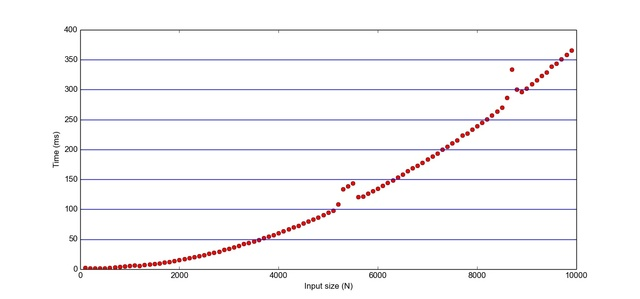
\includegraphics[scale=0.8]{./EJ3/resized2.jpg}
  \end{center}
  \vspace*{0.3cm}


\subsubsection[3.5]{Performance De Algoritmo y Gr\'afico}
Como mencionamos, nos interesa saber que heuristica de búsqueda local se adapta mejor a cada tipo de entrada estudiada con el algoritmo del ejercicio 2. Para esto, las enunciaremos nuevamente:

\begin{enumerate}
\item No se obtiene soluci\'on por no haber las pokeparadas necesarias para ganar en todos los gimnasios.
\item No se obtiene soluci\'on ya que la capacidad de la mochila no puede contener las pociones necesarias para vencer a un cierto gimnasio.
\item Todos los gimnasios sin necesidad de pociones para ser vencidos.
\item Las pokeparadas y los gimnasios se reciben en orden de la forma en la cual exista una pokeparada puntual para ir a cada gimnasio
\end{enumerate}

Veremos para cada una de las familias enunciadas, cual de las búsquedas locales nos provee una solución mejor a la solución provista por el algoritmo $greedy$. O en caso de no proveer ninguna solución, trataremos de dar respuesta a los motivos.

Para cada búsqueda local, se tomará una media alfa podada con $\alpha$ = 0.5 de manera de podar un 25\% de los datos a cada lado. De esta forma no habrá outliers en las muestras consideradas. 
La cantidad de mediciones para tomar la media será de 30. Además se tomará la varianza muestral usando la media calculada y las mediciones que queden luego de aplicar la media.\\

\subsubsection*{Familia 1}

\vspace*{0.3cm} \vspace*{0.3cm}
  \begin{center}
 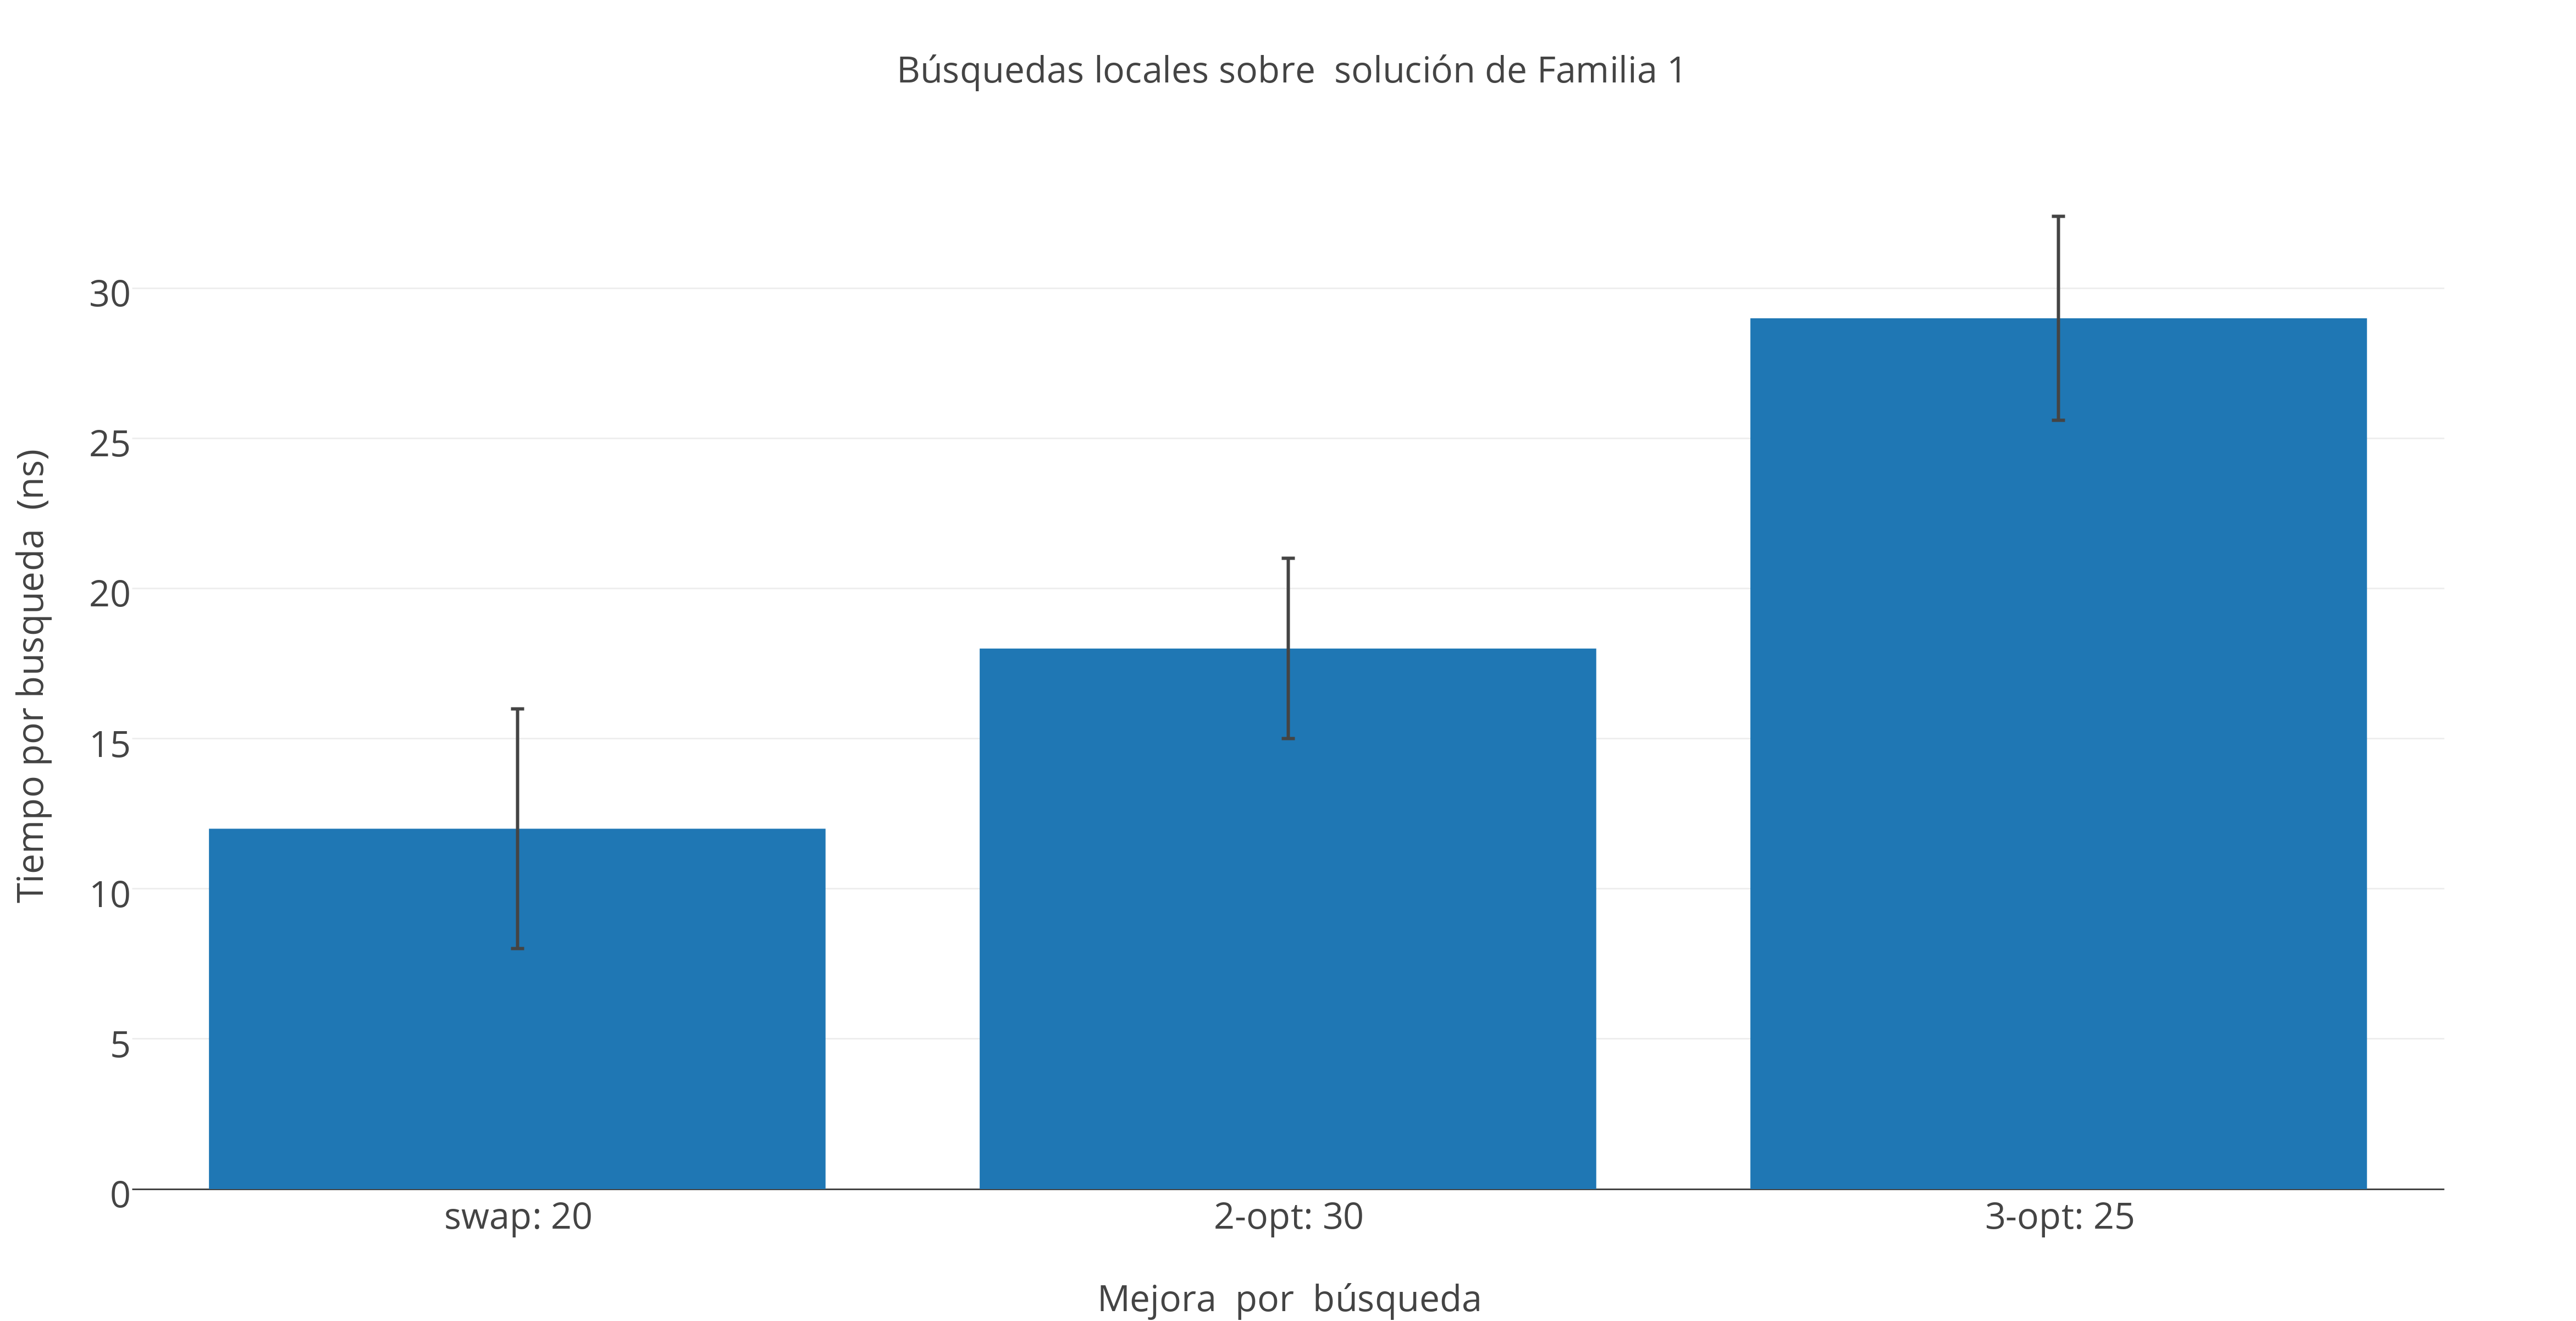
\includegraphics[scale=0.5]{./EJ3/local_search_familia.png}
 {            \textit{Gráfico \ 3.1 - Búsquedas locales sobre Familia 1}}
  \end{center}
  \vspace*{0.3cm}

\subsubsection*{Familia 2}

\vspace*{0.3cm} \vspace*{0.3cm}
  \begin{center}
 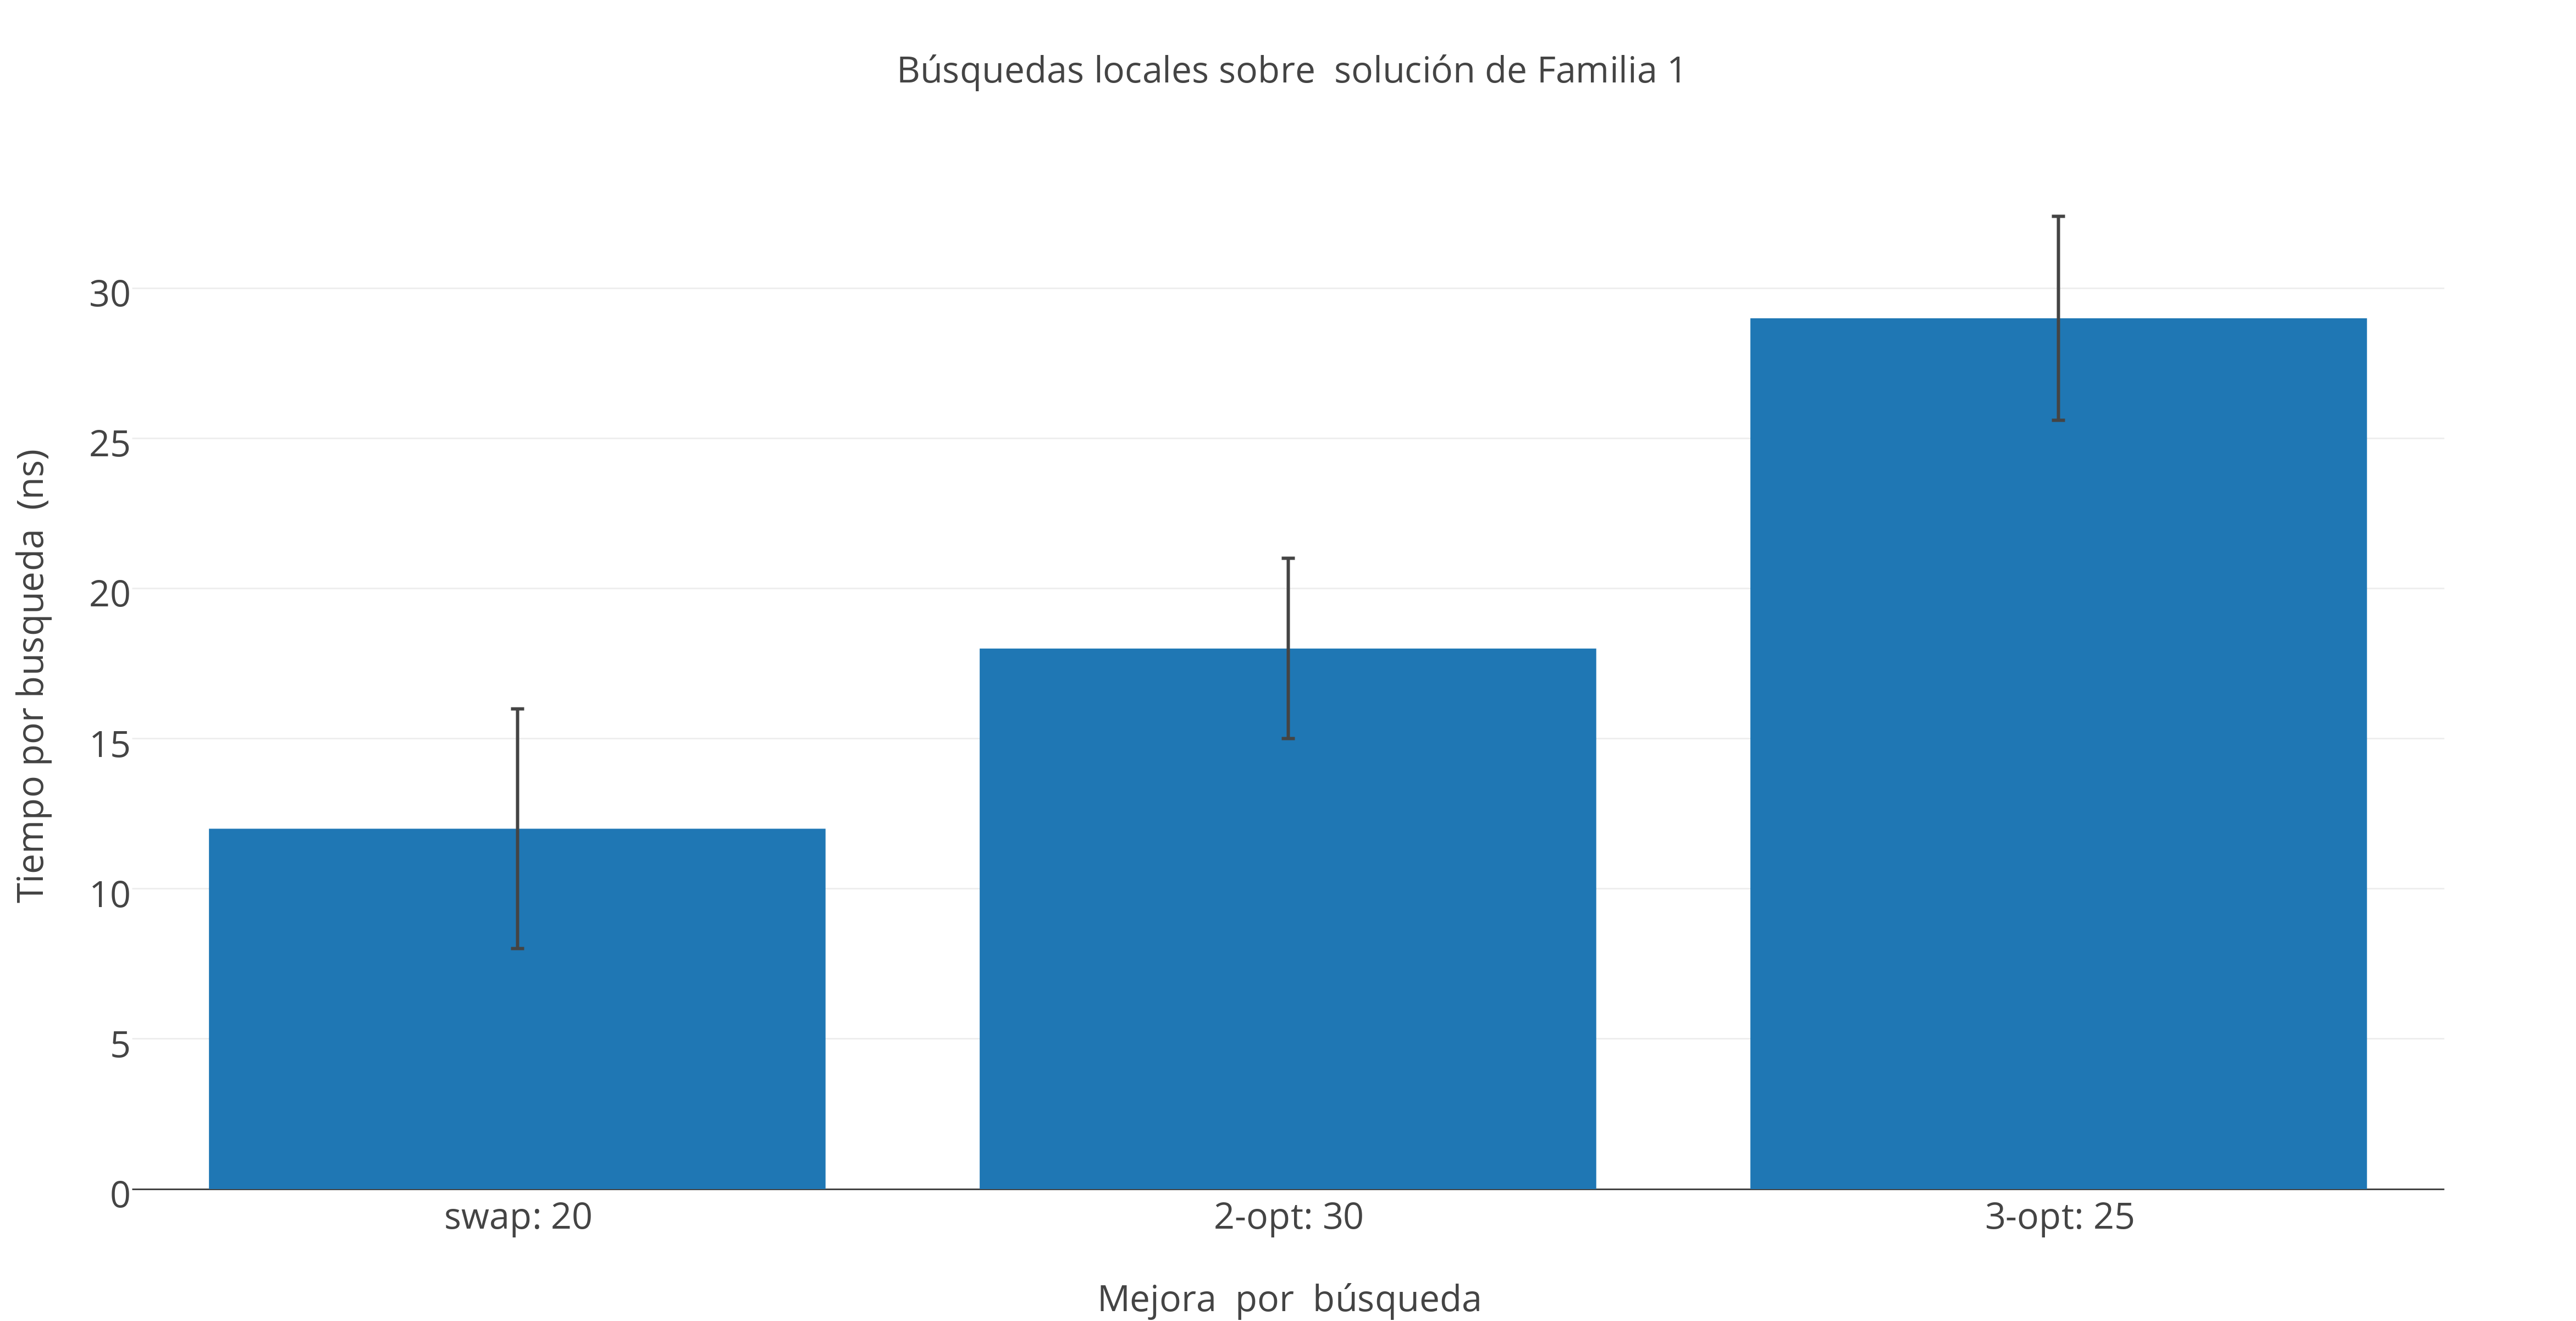
\includegraphics[scale=0.5]{./EJ3/local_search_familia.png}
 {            \textit{Gráfico \ 3.2 - Búsquedas locales sobre Familia 2}}
  \end{center}
  \vspace*{0.3cm}

\subsubsection*{Familia 3}

\vspace*{0.3cm} \vspace*{0.3cm}
  \begin{center}
 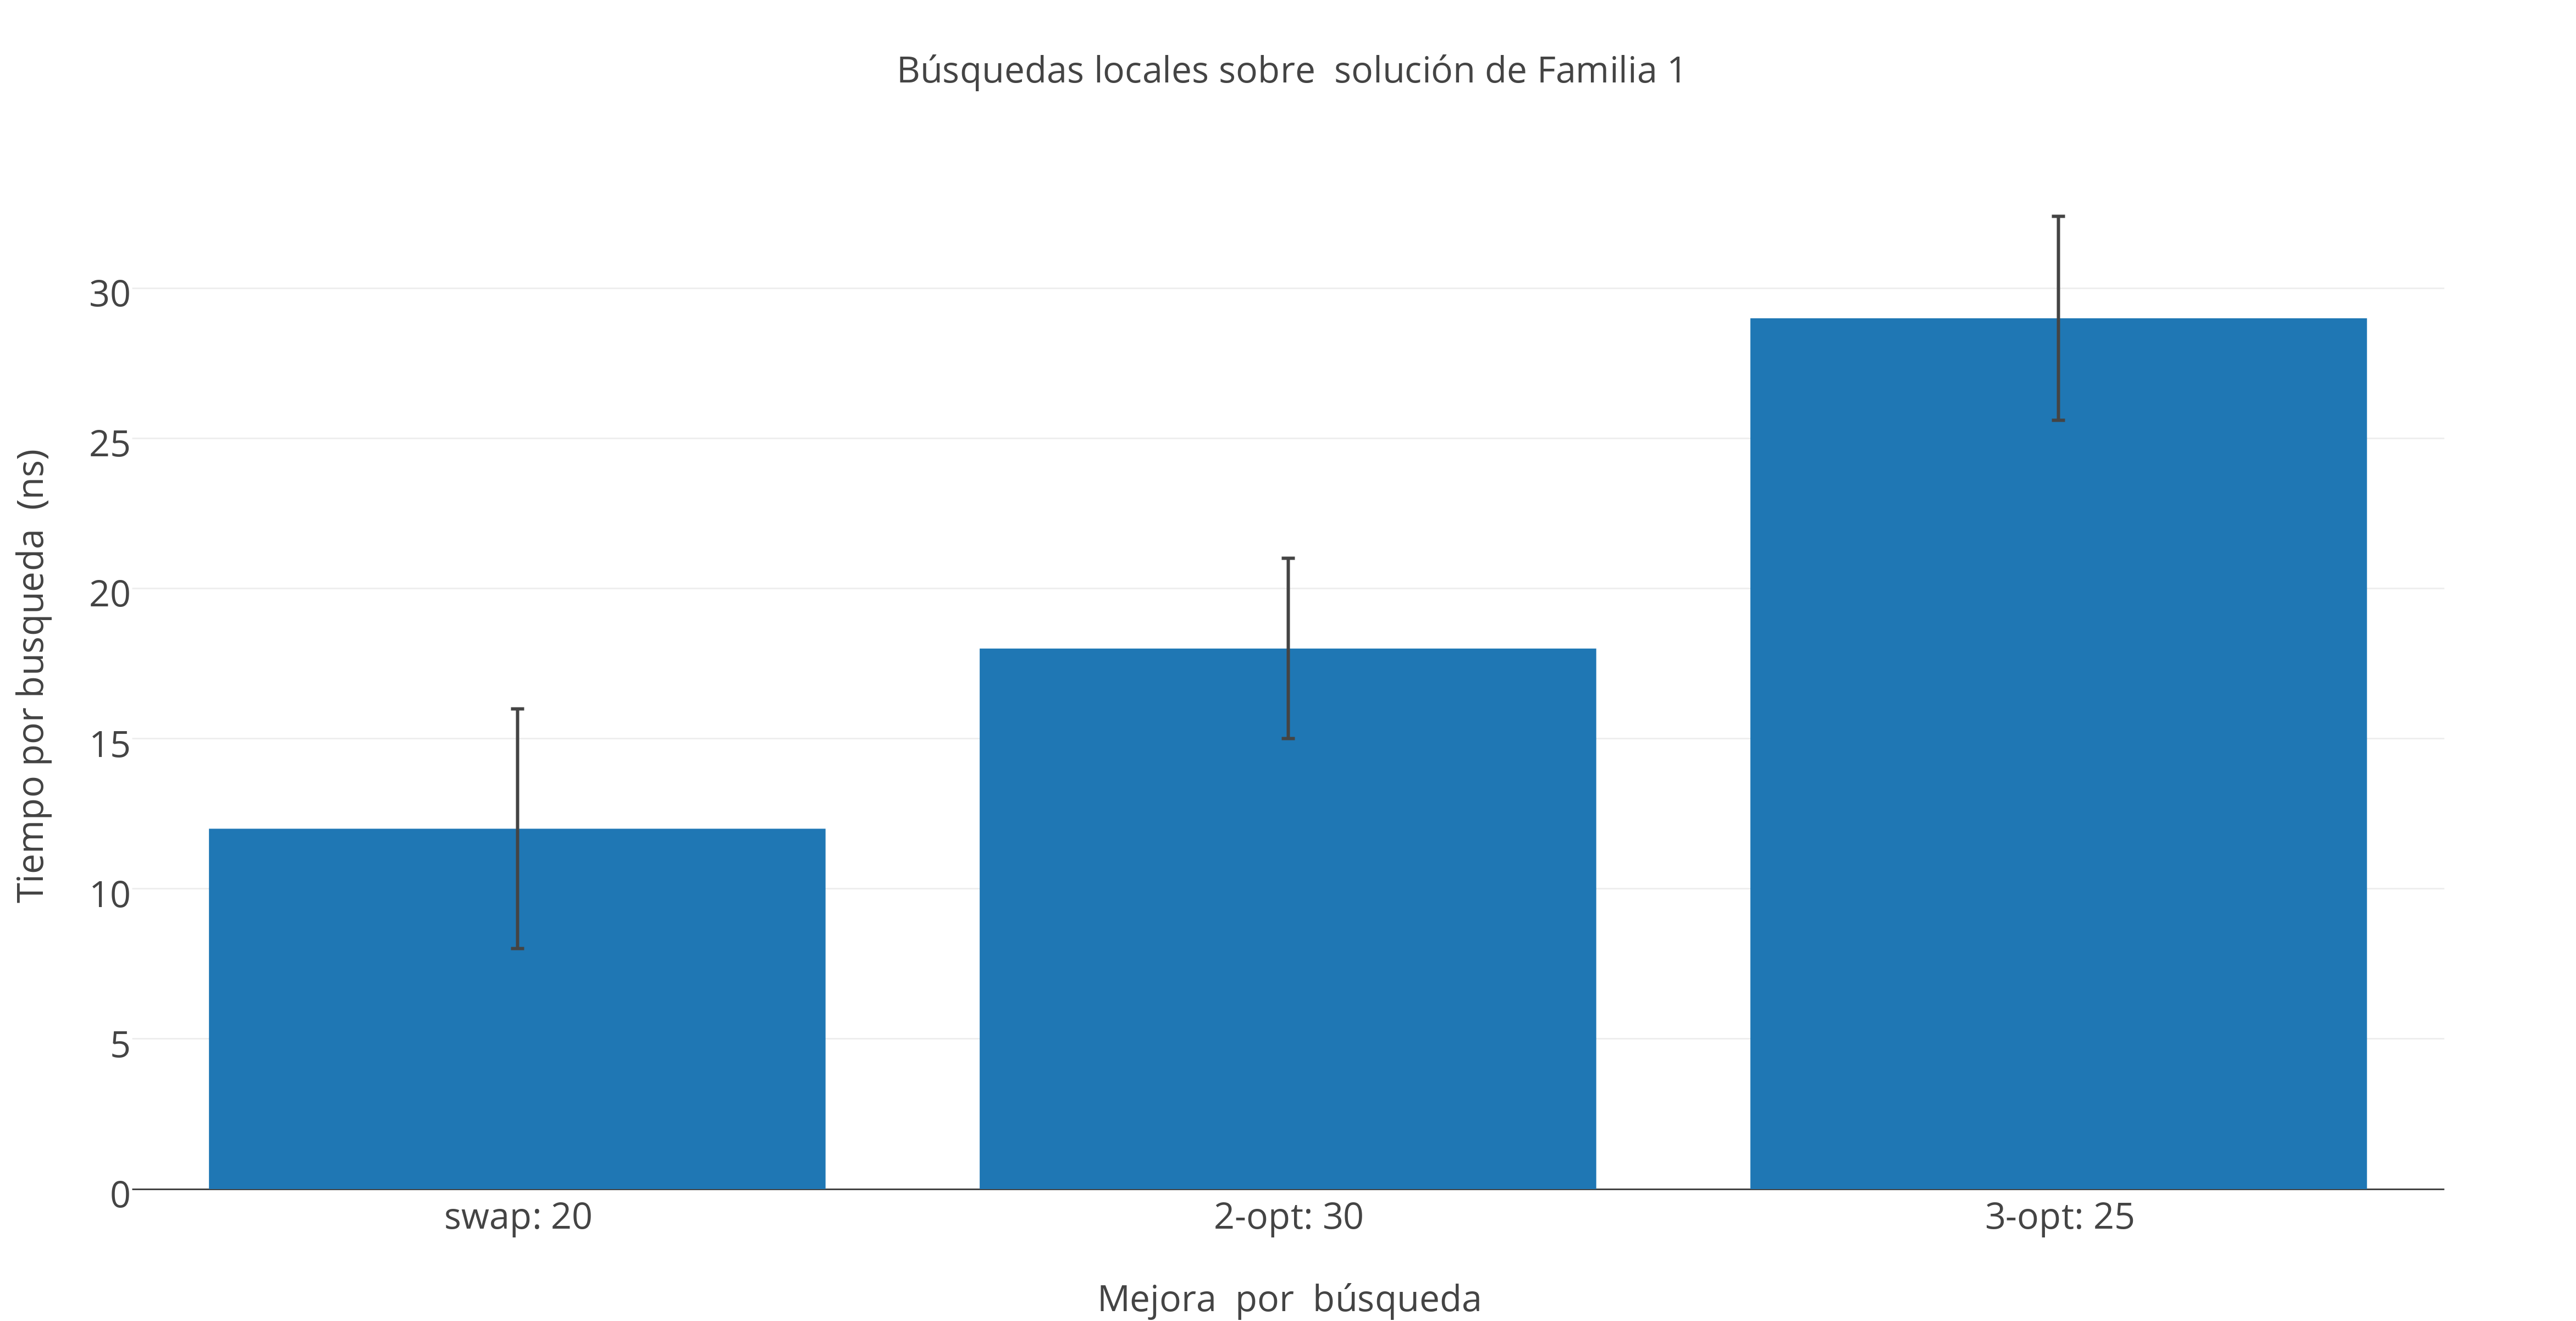
\includegraphics[scale=0.5]{./EJ3/local_search_familia.png}
 {            \textit{Gráfico \ 3.3 - Búsquedas locales sobre Familia 3}}
  \end{center}
  \vspace*{0.3cm}

\subsubsection*{Familia 4}

\vspace*{0.3cm} \vspace*{0.3cm}
  \begin{center}
 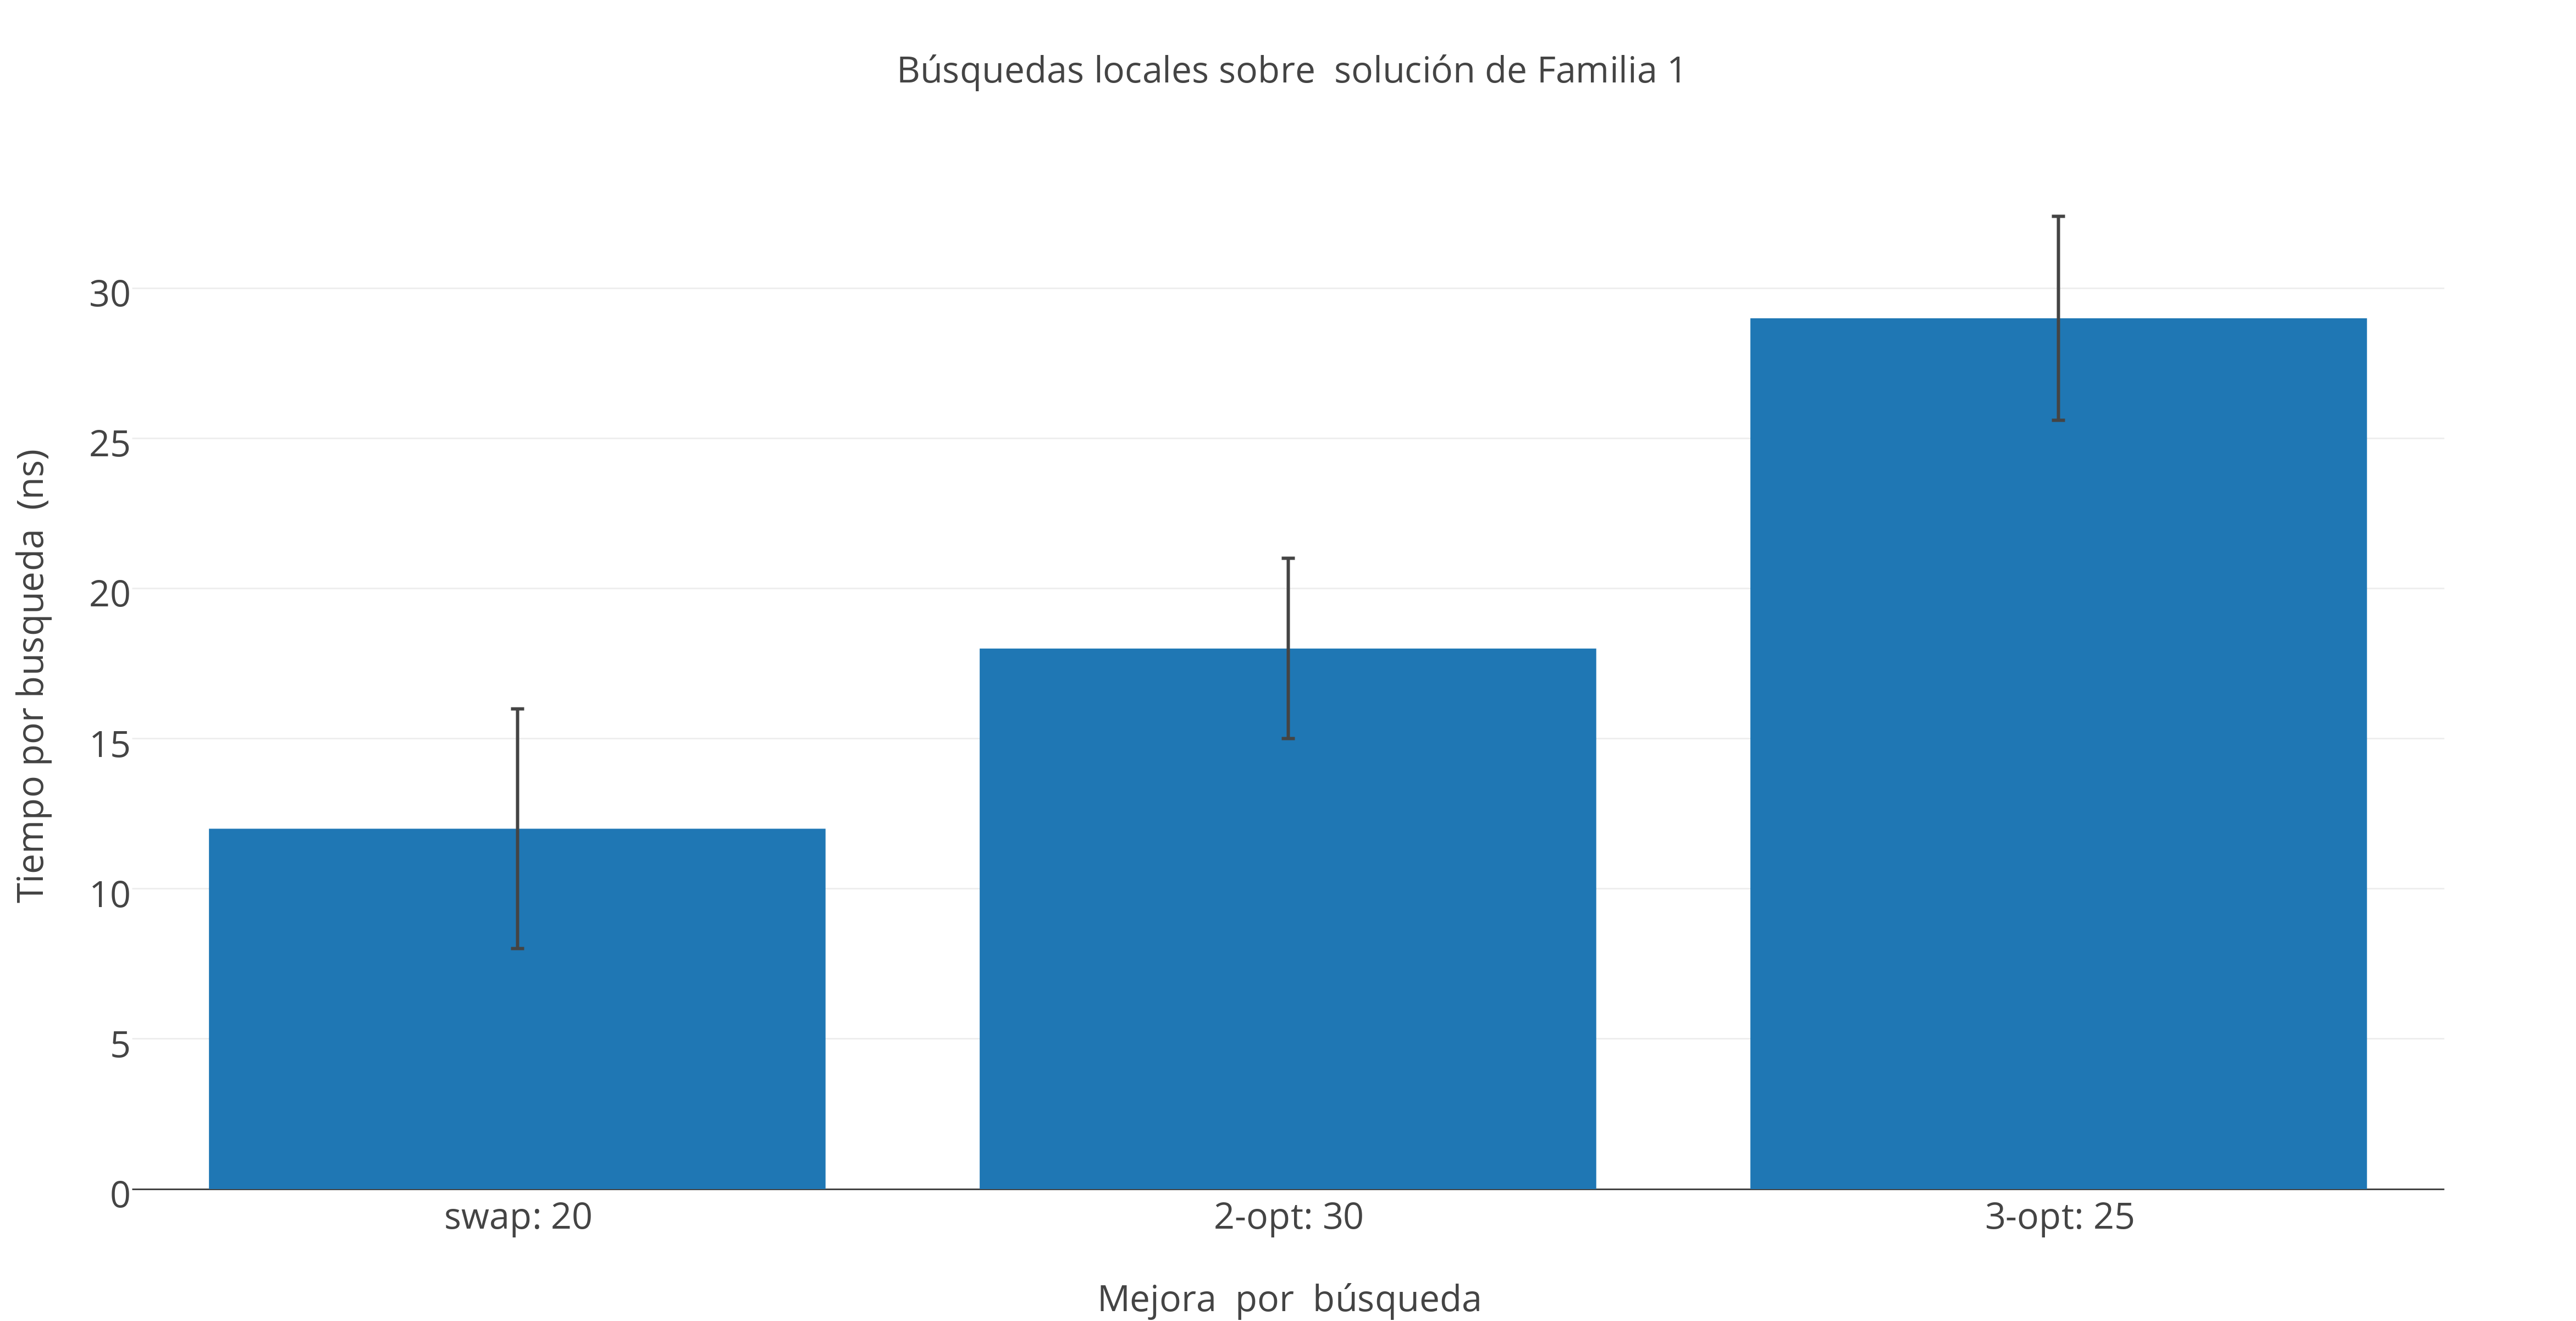
\includegraphics[scale=0.5]{./EJ3/local_search_familia.png}
 {            \textit{Gráfico \ 3.4 - Búsquedas locales sobre Familia 4}}
  \end{center}
  \vspace*{0.3cm}


\newpage
\section{Ejercicio 4} 
\subsection{Enunciado del problema}
Diseñar e implementar una heurística de búsqueda local para List Coloring y desarrollar los
siguientes puntos:

\begin{enumerate}
 \item Explicar detalladamente el algoritmo implementado. Plantear al menos dos vecindades distintas
para la búsqueda.
\item Calcular el orden de complejidad temporal de peor caso de una iteración del algoritmo de
búsqueda local (para las vecindades planteadas). Si es posible, dar una cota superior para la
cantidad de iteraciones de la heurística.
\item Realizar una experimentación que permita observar la performance del algoritmo comparando
los tiempos de ejecución y la calidad de las soluciones obtenidas, en función de las vecindades
utilizadas y elegir, si es posible, la configuración que mejores resultados provea para el grupo
de instancias utilizado.

\end{enumerate}

\subsection{Explicaci\'on de resoluci\'on del problema}
Como su nombre lo indica, búsqueda local analiza una vecindad local a la solución inicial $S_o$. Por lo que generalmente, la mejora obtenida puede no ser global, si no, la mejor solución dentro de la vecindad analizada. 

Para salir de un óptimo local, existen meta heurisiticas que pueden o no proveer una mejor solución observando otras vecindades, y en algunos casos acercarse lo suficiente u obtener el óptimo global. Una de ellas es la elegida para este informe, denominada, \textit{tab\'u search}.\\

La idea de esta meta heuristica es ir moviendose por las vecindades subyacentes a una vecindad analizada. Es decir, las vecindades de las soluciones que conforman una vecindad.
Pero no todas ellas, si no, la vecindad de una solución elegida que cumpla con ciertos atributos, o mejor dicho, que no posea ciertos atributos o caracteristicas. 
Esto es así, dado que se tiene que buscar una manera de descartar soluciones que no se consideren adecuadas para ser analizadas, si no, caeriamos en el problema de backtracking, donde se consideran todas las posibilidades, lo cual, puede ser impracticable.\\

Los atributos elegidos como no adecuados para elegir una solución son los denominados atributos \textit{tab\'u}. Existen muchas posibilidades según el problema estudiado. Para el problema del maestro pokemon eligiremos como atributos \textit{tabú} las aristas que sean modificadas al moverse de una solución a otra. Luego intentaremos ver que sucede al tomar como \textit{tabú} las aristas nuevas en la solución y ver si se obtienen mejores resultados.
Por lo tanto, se define un conjunto que alojará atributos \textit{tabú}.\\

Los métodos para encontrar vecindades serán los mismos analizados en el ejercicio tres. Es decir, a traves de las búsquedas locales estudiadas: $swap$, $2-opt$ y $3-opt$. Solo que para este algoritmo se filtrarán aquellos recorridos que no sean válidos. Luego una vecindad $V(s)$ para una solución $s$, será un conjunto de recorridos de soluciones válidas para el problema.\\

Debido a que la memoria tiene un limite, y los problemas podrian ser extremadamente grandes, se suele definir lo que se denomina \textit{tenor tabú} que es el tamaño máximo que el conjunto \textit{tabú} tiene para alojar atributos. Cuando el tamaño máximo es alcanzado, se tiene que determinar una manera de desalojar atributos para obtener espacio libre que pueda ser usado luego. El mótivo es tener una lista de tamaño acotado, pero que sea dinámica en contenido de atributos a lo largo de una corrida del algoritmo, dado que si no, al alcanzarse el tamaño máximo, la lista dejaria de crecer y los atributos dejarían de cambiar, acotando el universo de posibles soluciónes a la union de algunas vecindades.\\
Los atributos que serán desalojados serán aquellos que tengan más tiempo dentro del conjunto, por lo que además, el conjunto \textit{tabú} tendrá la caracteristica de poder contener esa información y funcionar internamente como pila. 
La cantidad de atributos desalojados será determinada por la cantidad de atributos que se quiera alojar en el conjunto. En el peor caso, todos los atributos serán nuevos.\\

Además, si el tenor definido en el punto anterior es lo suficientemente grande, indefectiblemente, en algún punto tendremos todos los atributos alojados. Por lo cual tendremos que tomar alguna decision para elegir una nueva solución en la vecindad analizada. Esta decision se conoce como función de aspiración $A(V(s)): \rightarrow s^{'}$ que dada una vecindad $V(s)$ a una solución $s$, determina que solución tomar.
La decision puede tomarse en base a la cantidad de atributos \textit{tabú} que posee la solución analizada. Luego puede elegirse la más tabú o la menos tabú.
En este informe estudiarmos ambas metodologias y veremos cual nos ofrece mejores resultados.\\




 
 
\subsection{An\'alisis de complejidades}
Con la idea utilizada en la demostración de finalización de nuestro algoritmo podemos generar una cota para la complejidad de los algoritmos planteados en esta sección. \\
Si en nuestro algoritmo realizamos $K$ pasadas, quiere decir que mejoramos la solución en $K - 1$ pasadas, es decir, aumentamos la cantidad de aristas buenas en $K - 1$ pasadas. Como la cantidad de aristas buenas es como mínimo $0$ y como mucho $E$ y en cada pasada aumentamos en al menos $1$ la cantidad de aristas buenas, realizamos como mucho $O(E)$ pasadas. \\
Como en cada pasada, iteramos los $V$ nodos, esto nos da que la complejidad de los algoritmos es $O(E * V * X)$ donde $X$ es lo que cuesta procesar un nodo en particular para intentar mejorar la solución. \\

Para la primer vecindad, en el peor de los casos probamos con todos los colores. Probar con un color hace tantas operaciones como vecinos tenga un nodo, por lo que es $O(E)$, como lo hace para cada color, la complejidad termina siendo $O(E^2 * V * C)$, con  $C$ la cantidad total de colores. La complejidad de una iteración resulta $O(V * E * C)$\\

Para la segunda vecindad, calcular el mejor color y setearlo tiene costo $O(E)$ (hace tantas operaciones como vecinos tenga), por lo que la complejidad termina siendo $O(E^2 * V)$. La complejidad de una iteración resulta $O(V * E)$. \\

\subsection{Experimientos y conclusiones}
\subsubsection[3.5]{Test}
Queremos observar que tan bueno es el algoritmo propuesto en la práctica. Para esto realizaremos una serie de tests utilizando las entradas que se utilizaron en el ejercicio 3.
La idea es tratar de encontrar la configuración ideal para que en promedio el algoritmo resuelva la mayoria de los casos eficientemente. Para lograr esto, experimentamos variando distintos parametros para cada entrada y obtener las respectivas conclusiones de los resultados obtenidos.\\
Los parámetros de estudio fueron:

\begin{enumerate}
\item  \textbf{Cantidad de iteraciones}: Tenemos que observar en promedio, cuantas iteraciones conviene tomar para obtener un buen resutado.
\item \textbf{Tenor tabú}: Tenemos que observar que sucede al aumentar el tenor tabú, y hasta cuanto es conveniente hacerlo para obtener un buen resultado.
\item \textbf{Atributos tabú}: Analizar que sucede al tomar como atributos tabú las aristas que cambiaron o las aristas nuevas
\item \textbf{Función de aspiración}: Elegir la solución más tabú o la menos tabú.
\end{enumerate}

Debemos aclarar, que tenor tabú fué establecido en cantidad de pokeparadas mas gimnasios. Este valor puede ser relativamente grande, pero cuanto más grande, más tiempo de resolución es necesario, con lo cual al final no es una cuestion de memoria, si no, una cuestion de tiempo de computos necesaria para correr el algoritmo.
También se trabajó probando diferentes configuraciones de atributos tabú y función de aspiración, obteniendo en todos los casos los mismos resultados, por lo que al final se decidió dejar prefijado el estandar para tabú search que es aristas viejas como atributos tabú y solución menos tabú para la función de aspiración.\\

Se tomaron 20 mediciones por cada tipo de test y se tomó una media alfa podada de las mismas con $\alpha$ = 0.5 de manera de podar un 25\% de los datos a cada lado.  De esta forma se reduce la posibilidad de outliers en las muestras consideradas.

Como fue enunciado en incisos anteriores de este trabajo las 4 familias en las que la heur\'istica golosa no otorga una soluci\'on \'optima son:

\begin{enumerate}
\item Familia 4
\item Familia 6
\item Familia 7
\item Familia 8
\end{enumerate}

Estas ser\'an las únicas a ser a analizadas, ya que el resto son el resultado exacto o no tienen soluci\'on, con lo cual no aportan mayor relevancia.
 
\subsubsection*{Familia 4}

Veamos algunos resultados de aplicar cada version de tabú search:

\vspace*{0.3cm} \vspace*{0.3cm}
  \begin{center}
 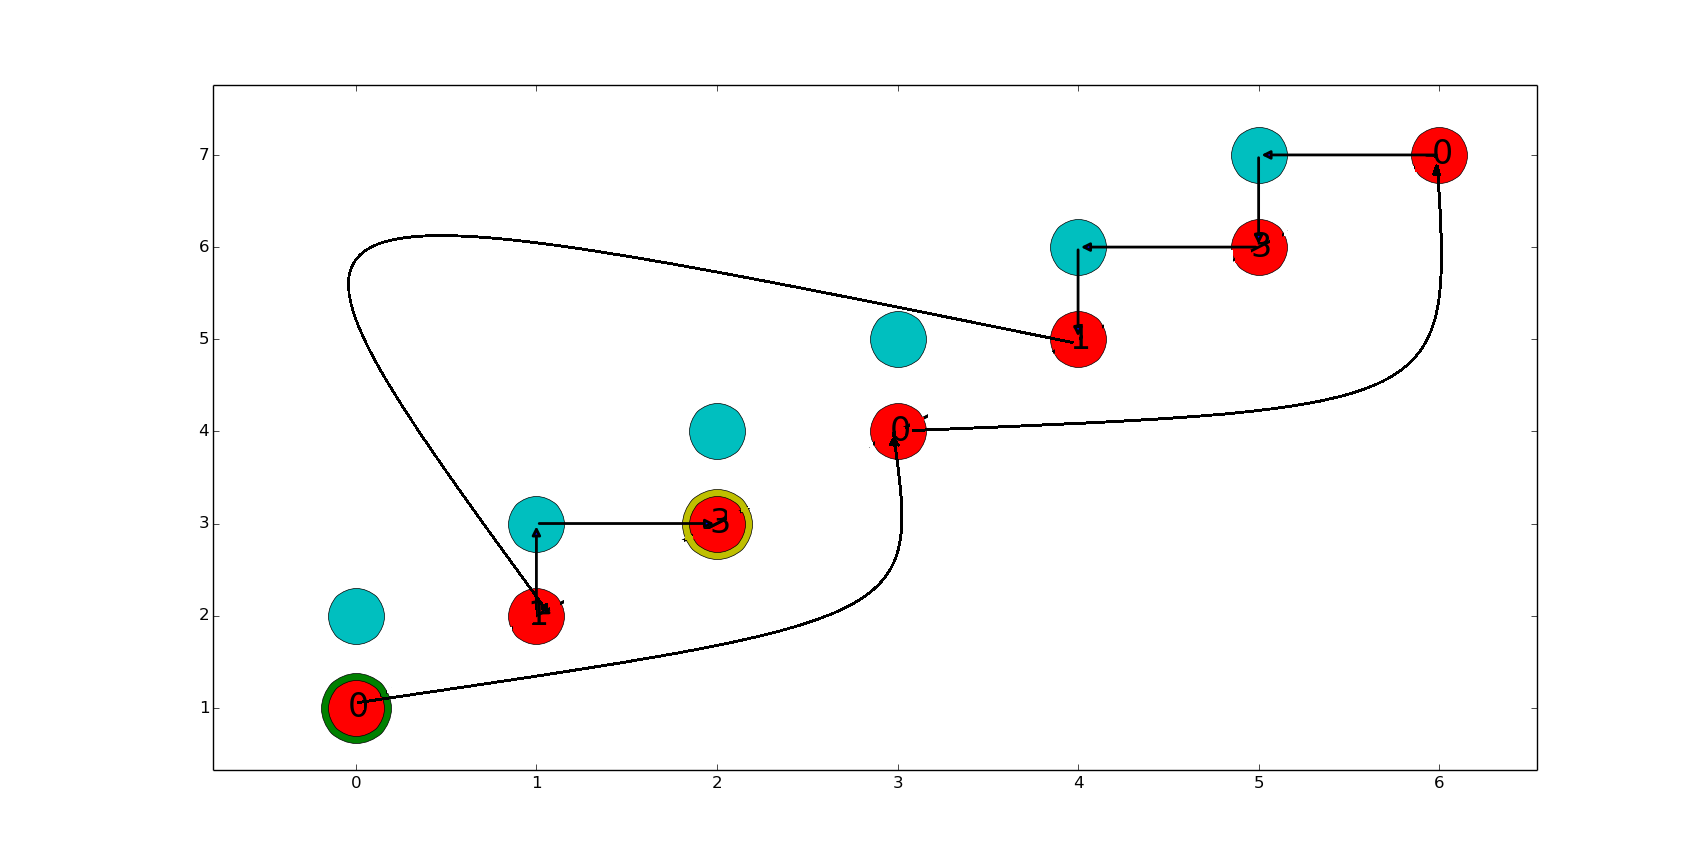
\includegraphics[scale=0.3]{./EJ4/fam4goloso.png}\\
 {            \textit{Soluci\'on Golosa}}
  \end{center}
  \vspace*{0.3cm}

\vspace*{0.3cm} \vspace*{0.3cm}
  \begin{center}
 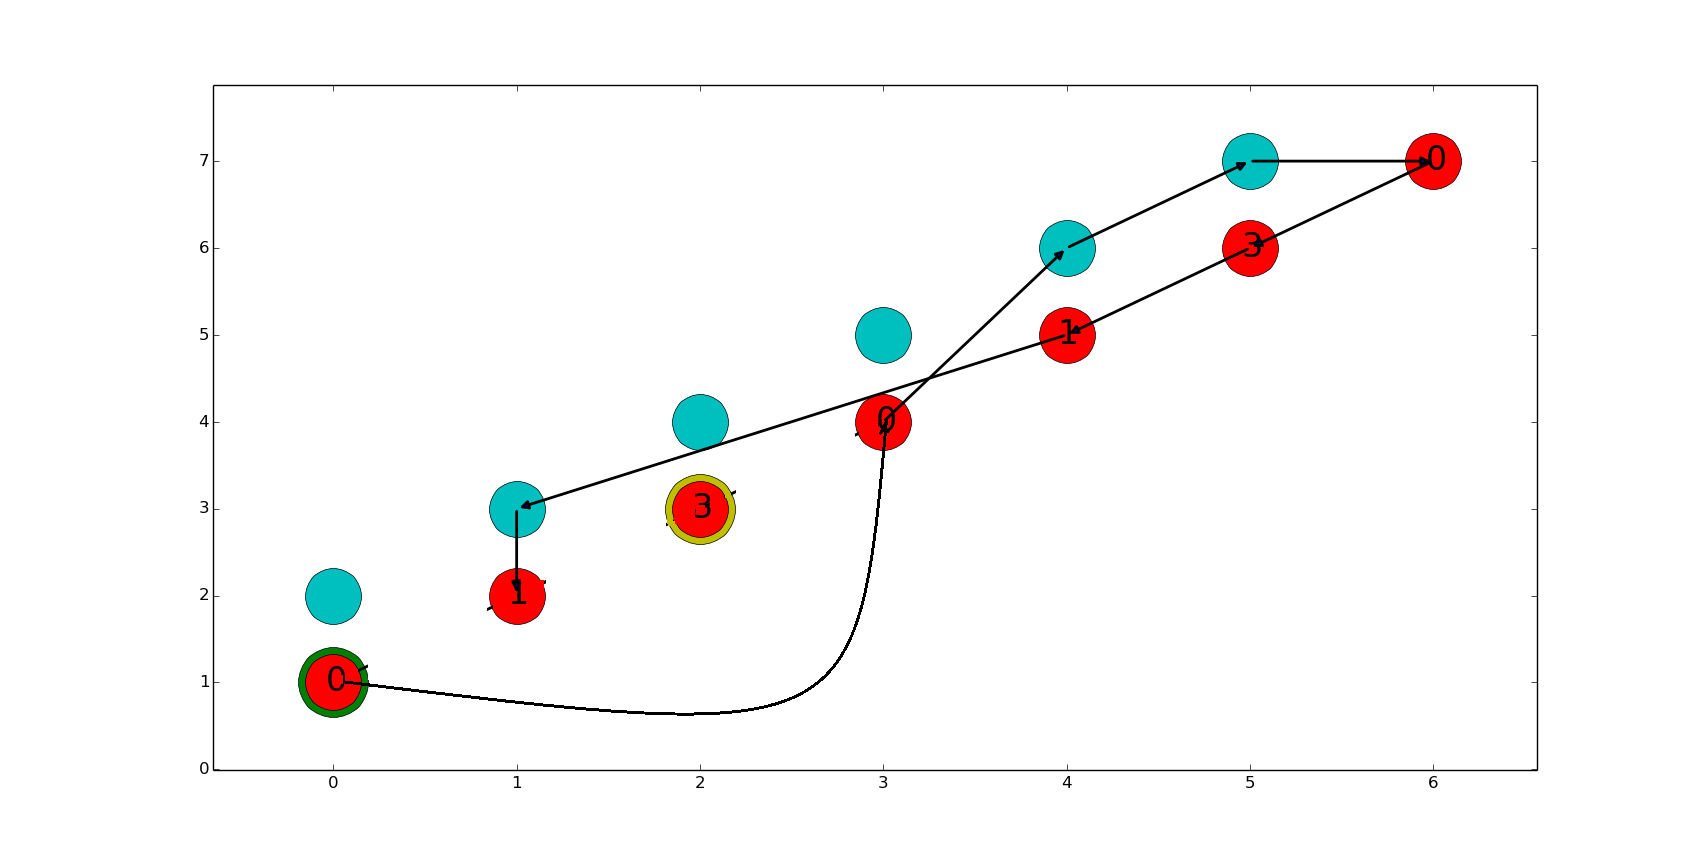
\includegraphics[scale=0.3]{./EJ4/fam42opt.png}\\
 {            \textit{Soluci\'on 2-OPT}}
  \end{center}
  \vspace*{0.3cm}

\vspace*{0.3cm} \vspace*{0.3cm}
  \begin{center}
 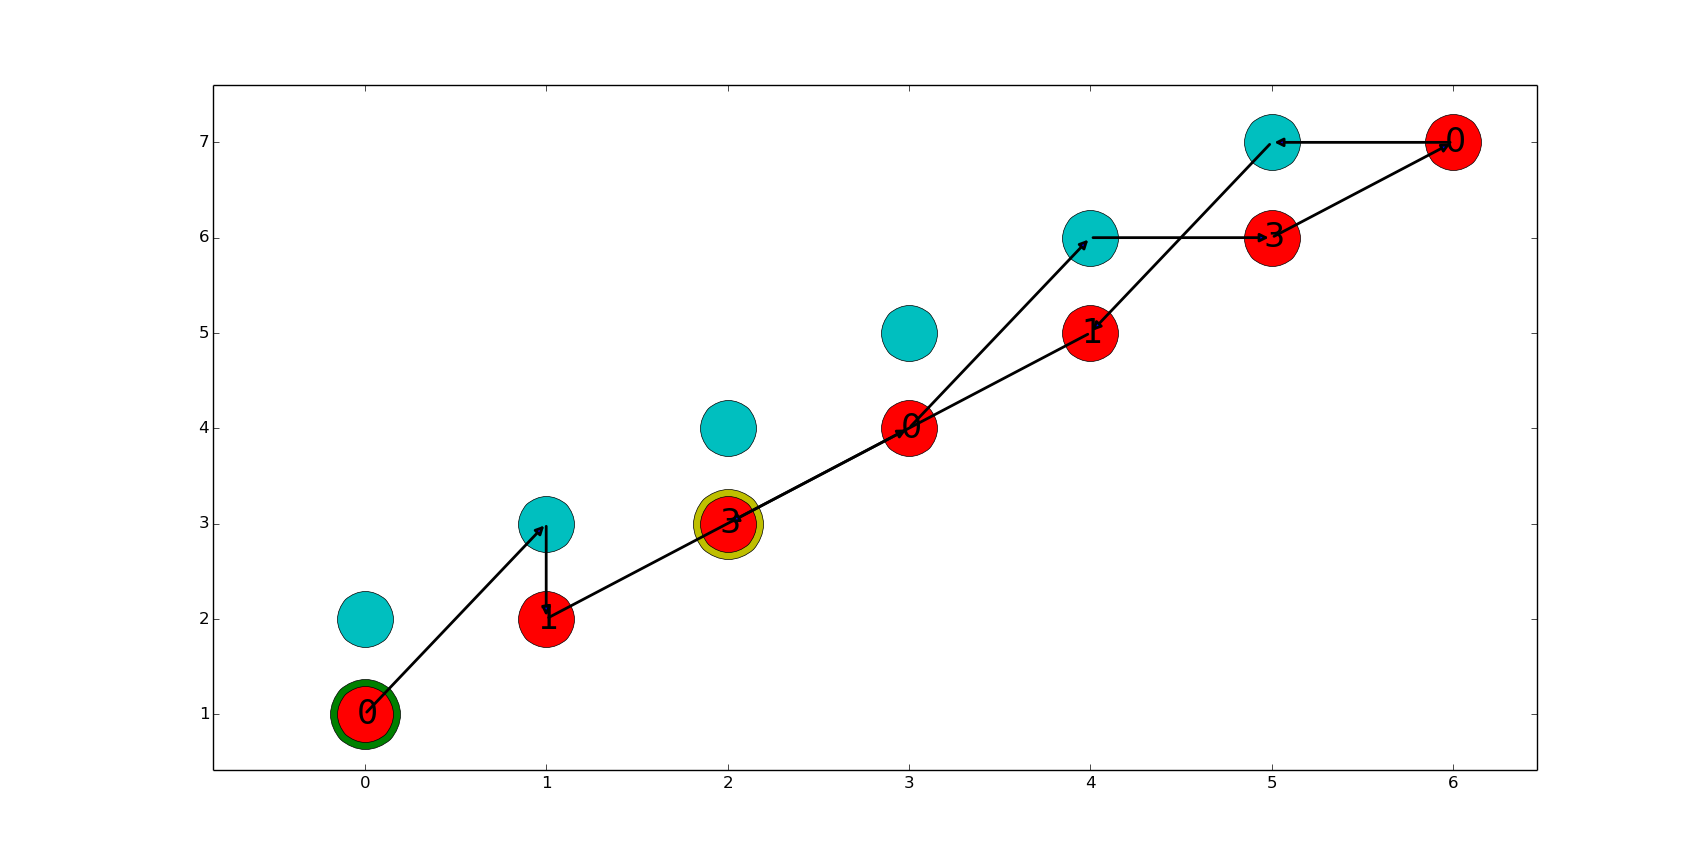
\includegraphics[scale=0.3]{./EJ4/fam43opt.png}\\
 {            \textit{Soluci\'on 3-OPT}}
  \end{center}
  \vspace*{0.3cm}

Nos parece interente comparar los resultados de mejora y tiempo de las búsquedas locales y tabú search que utilicen la misma vecindad, para ver si tabú search mejora lo logrado por la búsqueda local o empeora el resultado. Esto será realizado para cada familia mencionada.\\

Veamos como se comporta tabú 2-OPT con respecto a la heuristica de búsqueda local 2-OPT dentro de la familia 4:

\vspace*{0.3cm} \vspace*{0.3cm}
  \begin{center}
 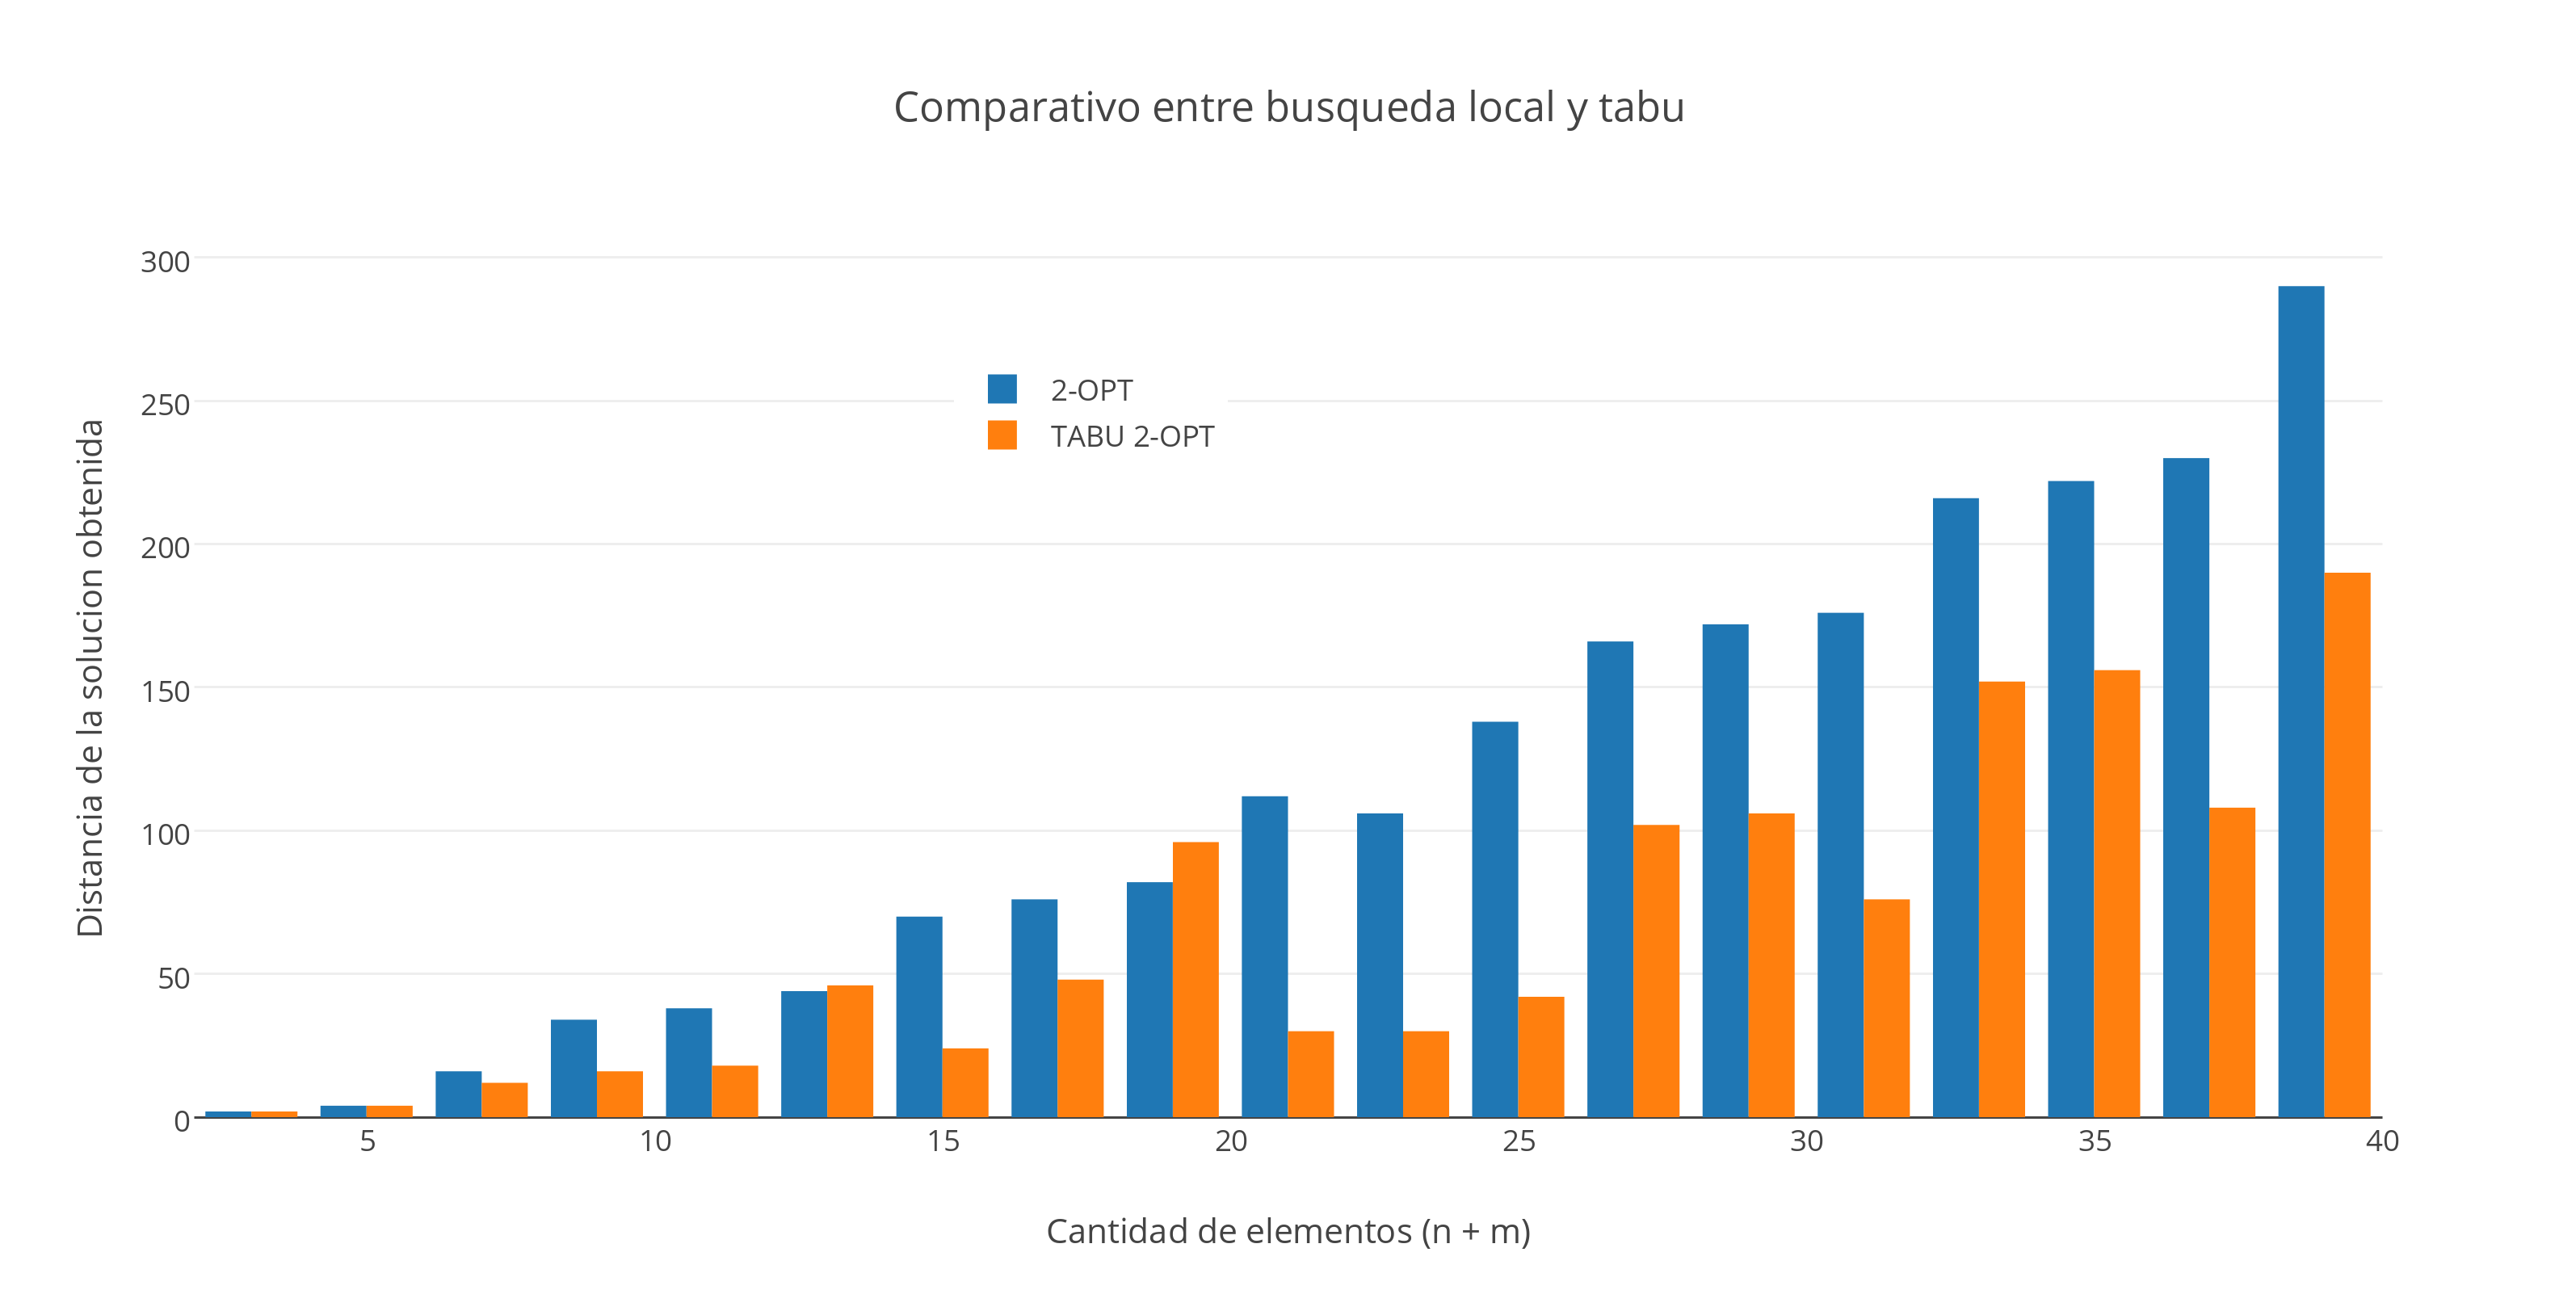
\includegraphics[scale=0.5]{./EJ4/comparativogym02opt.png}\\
 {            \textit{Gráfico \ 4.1 - 2-OPT vs Tabu 2-OPT sobre Familia 4}}
  \end{center}
  \vspace*{0.3cm}

En cuanto a tiempo insumido vemos lo siguiente:

\vspace*{0.3cm} \vspace*{0.3cm}
  \begin{center}
 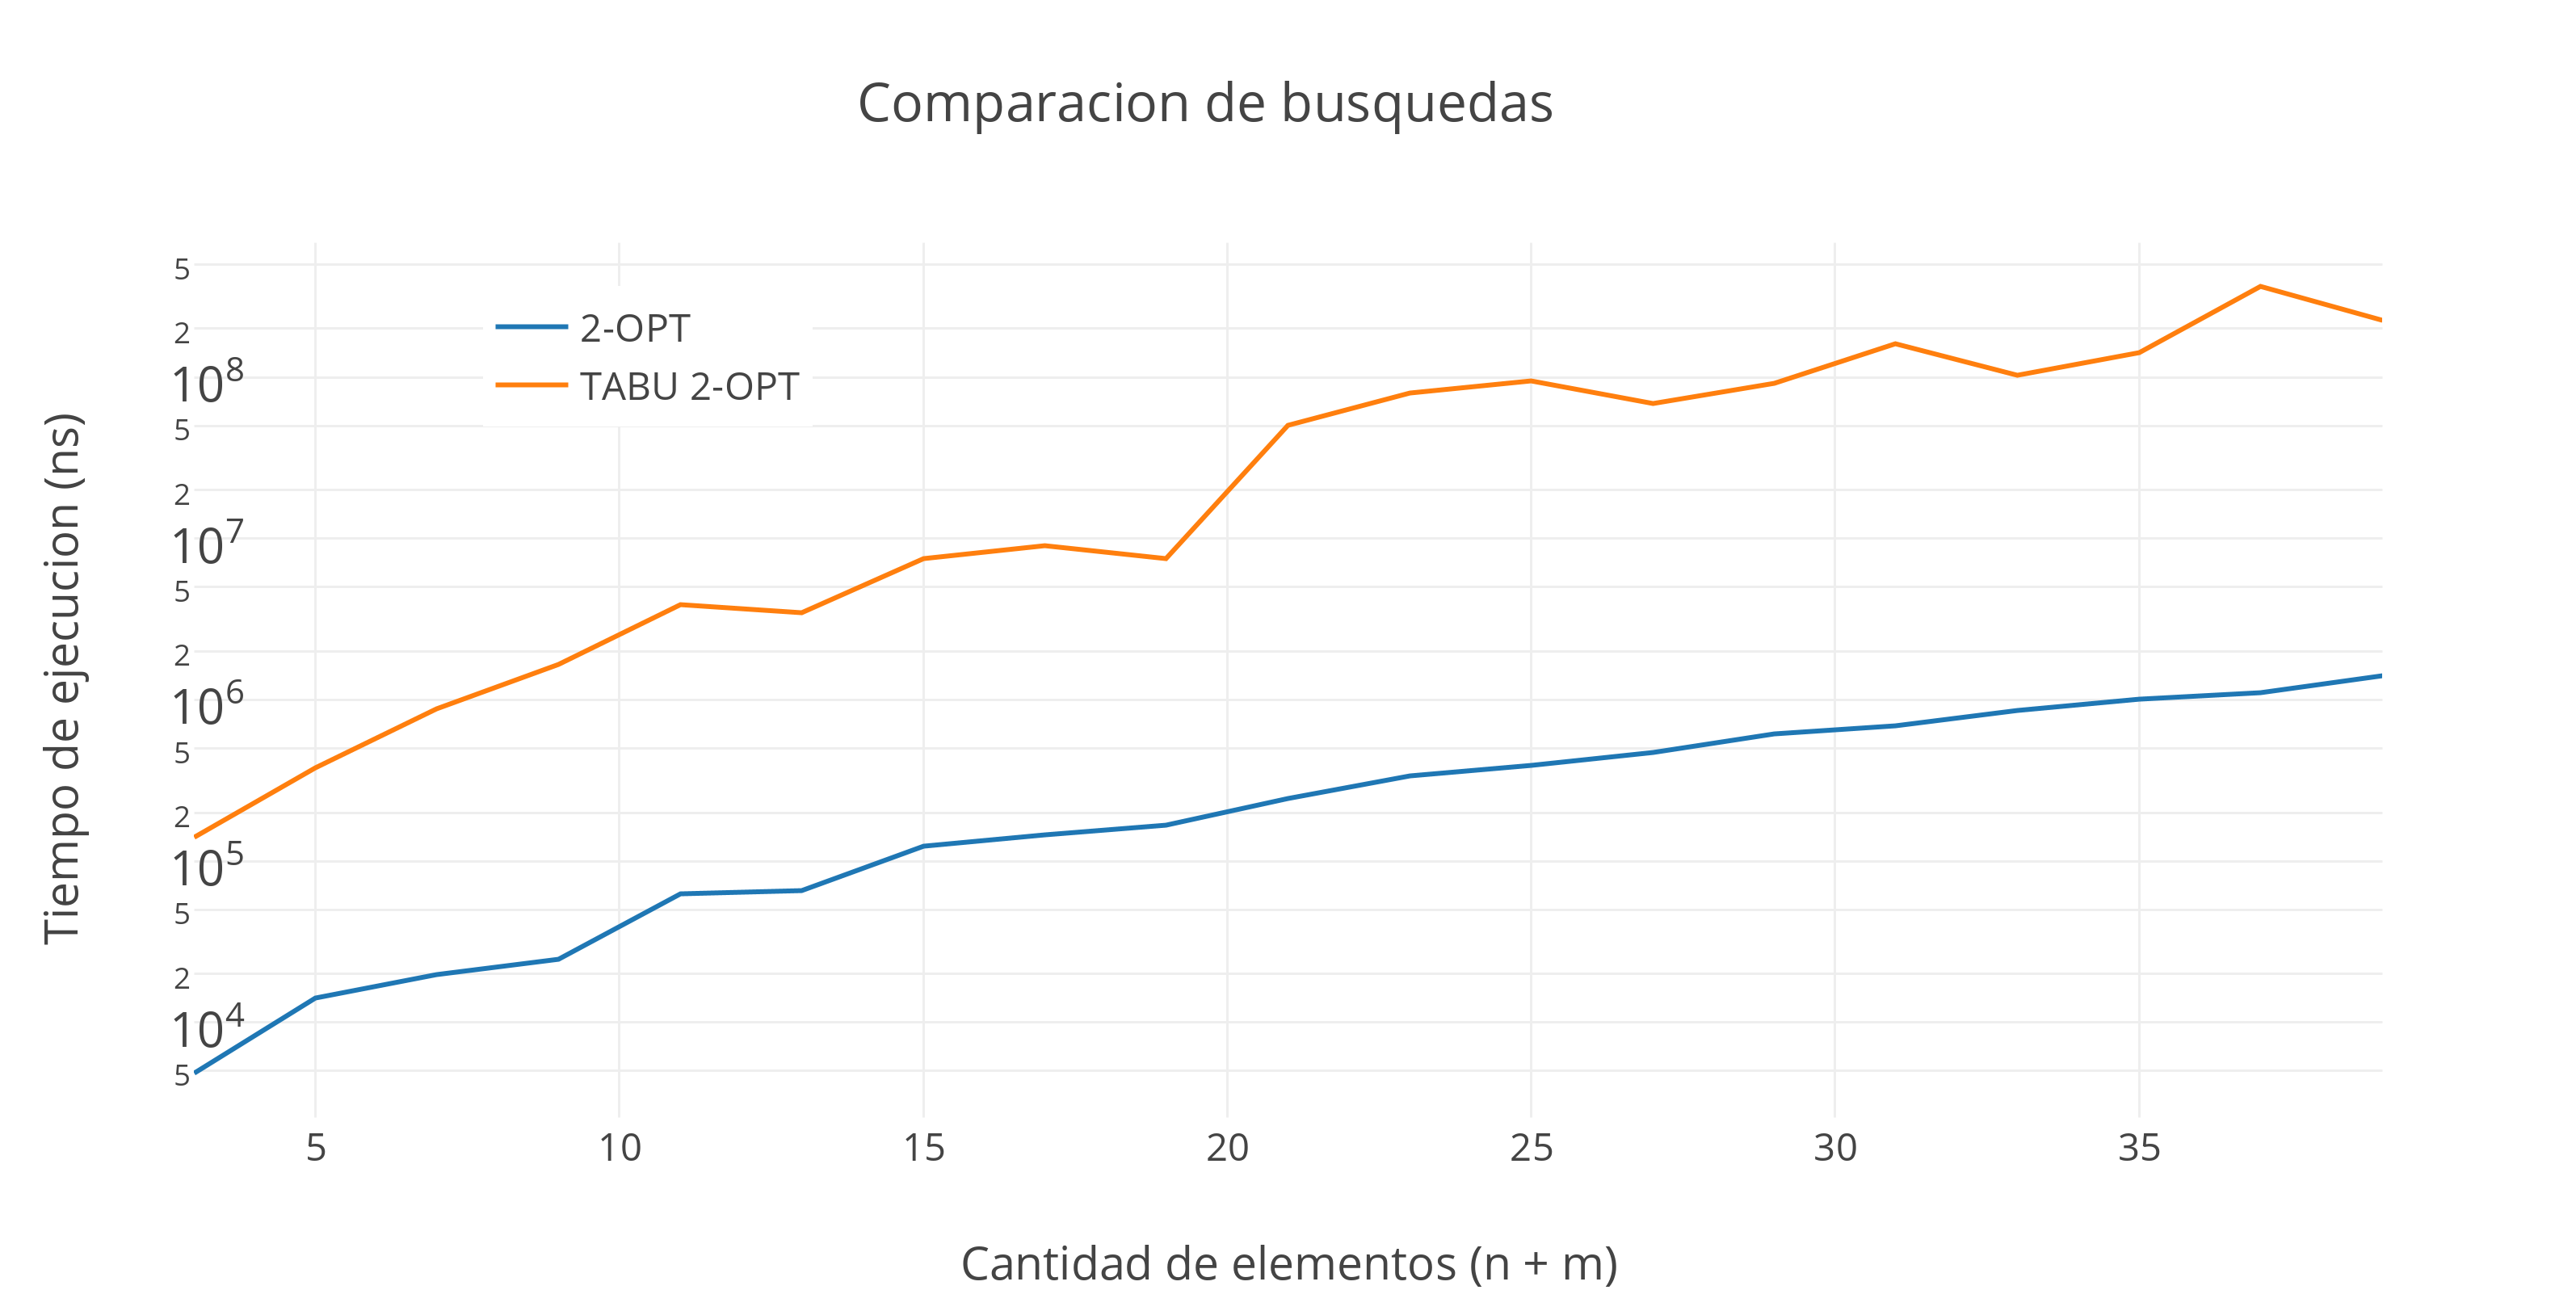
\includegraphics[scale=0.5]{./EJ4/medicion2optgym0.png}\\
 {            \textit{Gráfico \ 4.2 - 2-OPT vs Tabu 2-OPT sobre Familia 4}}
  \end{center}
  \vspace*{0.3cm}
  
 Aplicando 3-OPT:

\vspace*{0.3cm} \vspace*{0.3cm}
  \begin{center}
 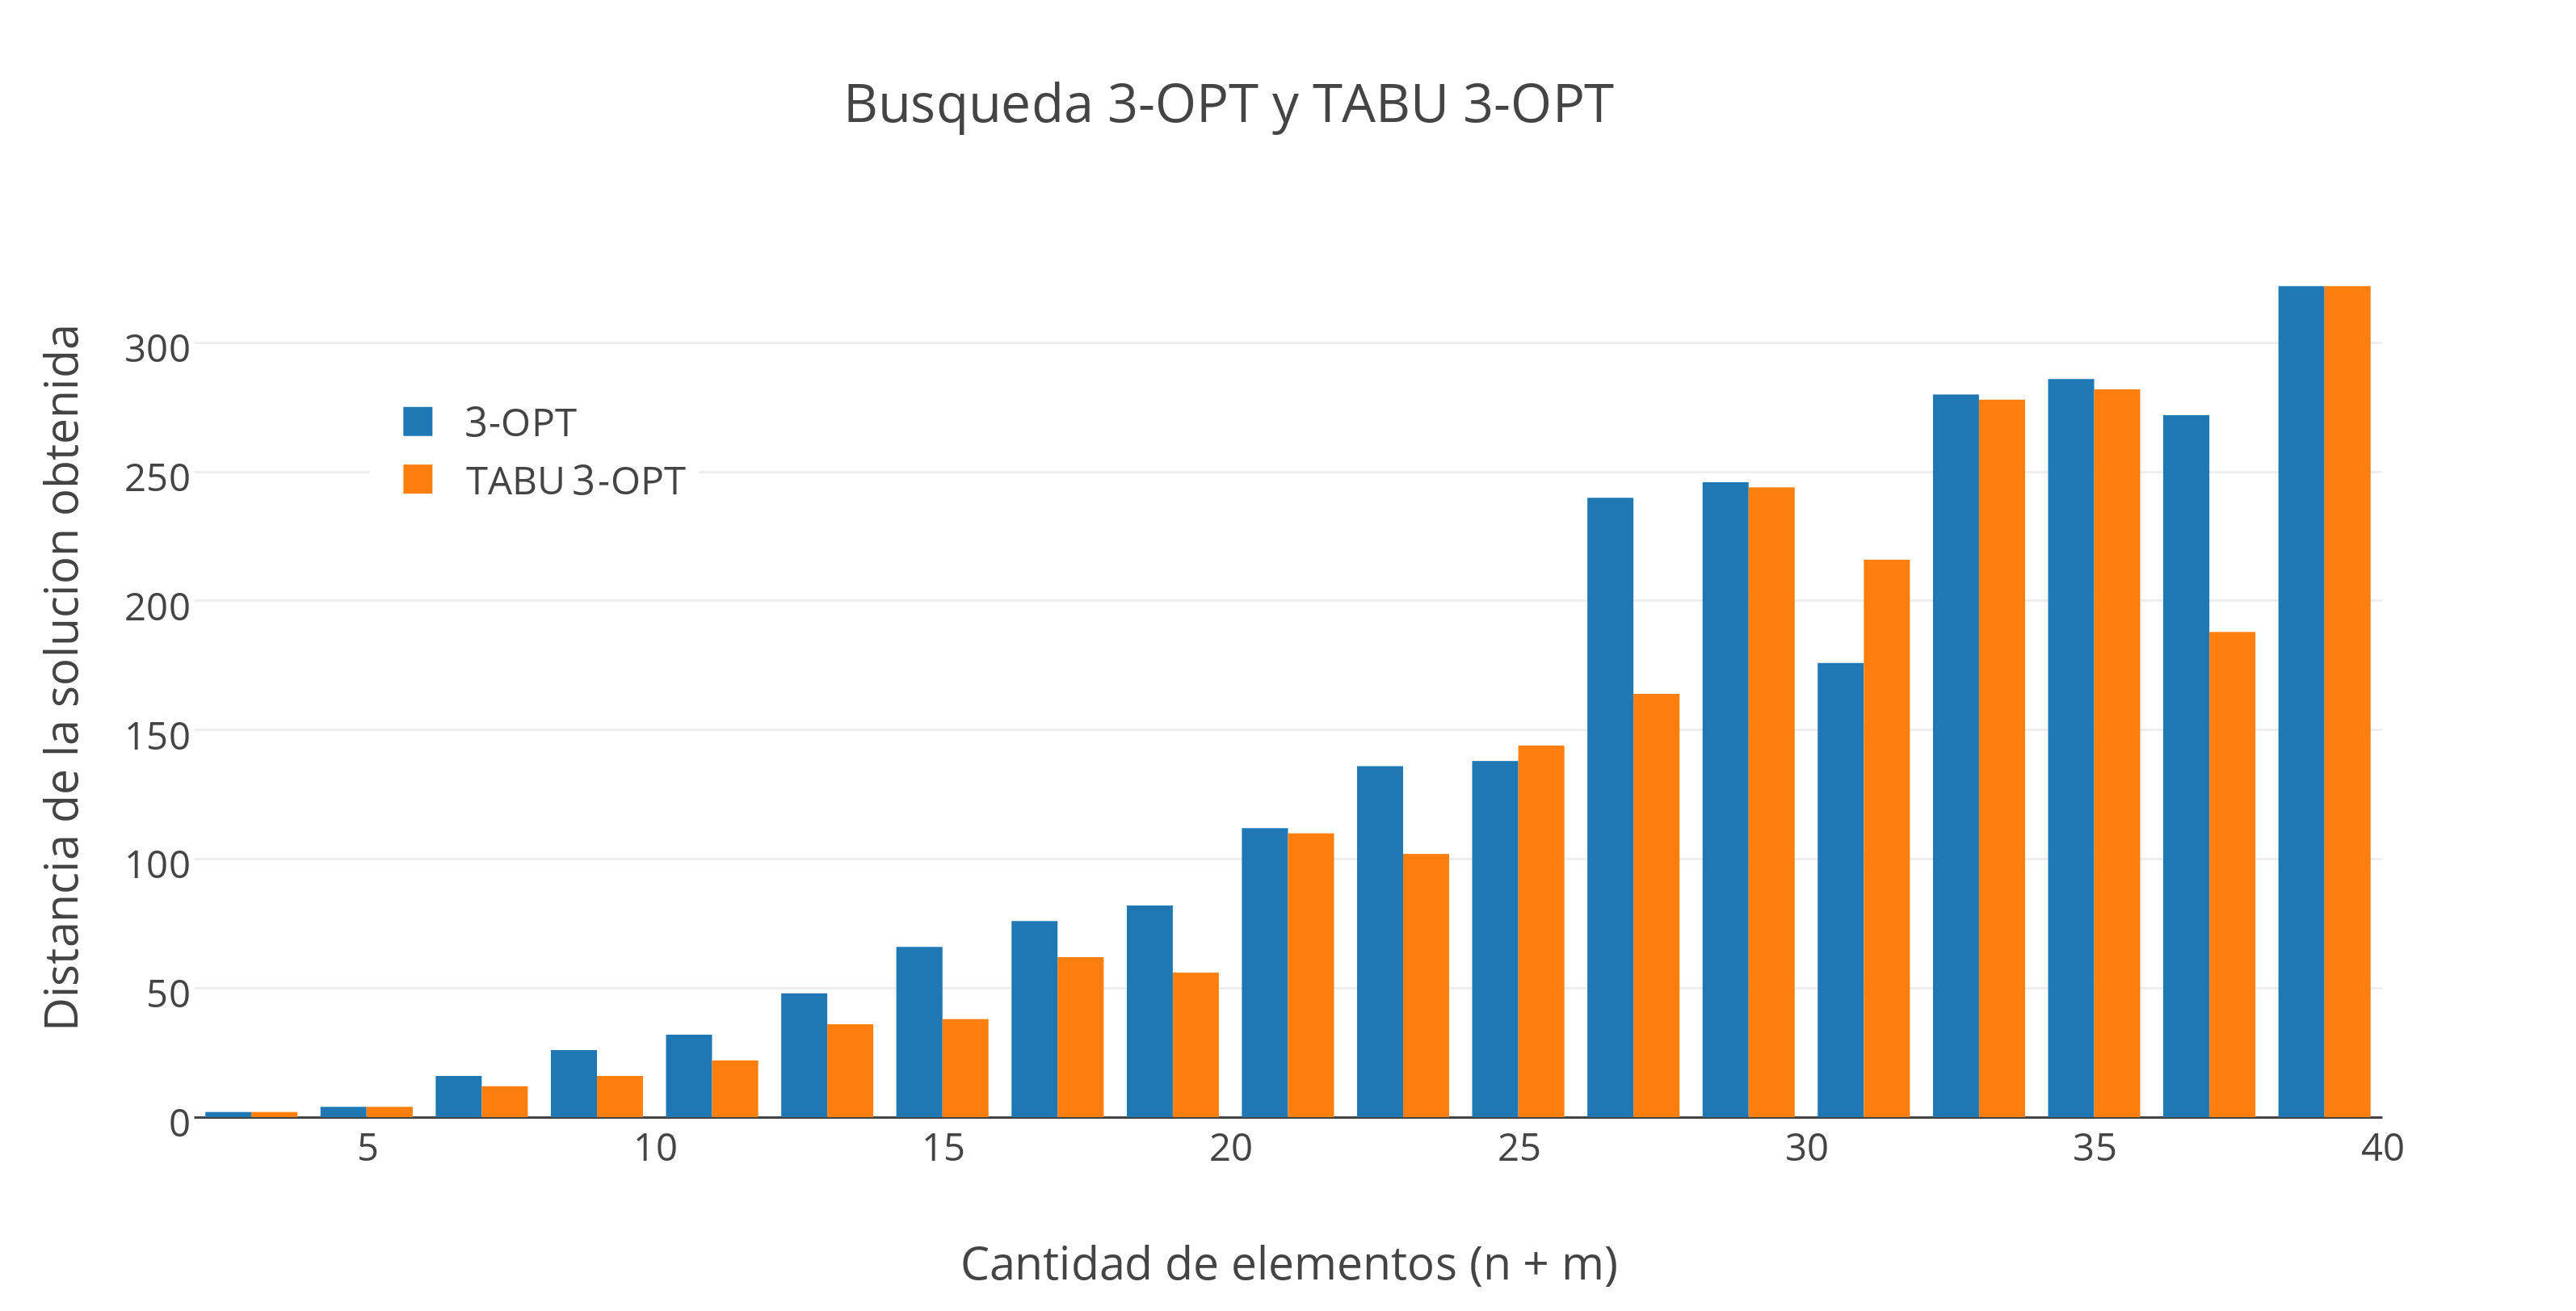
\includegraphics[scale=0.5]{./EJ4/comparativogym03opt.png}\\
 {            \textit{Gráfico \ 4.3 - 3-OPT vs Tabu 3-OPT sobre Familia 4}}
  \end{center}
  \vspace*{0.3cm}

\vspace*{0.3cm} \vspace*{0.3cm}
  \begin{center}
 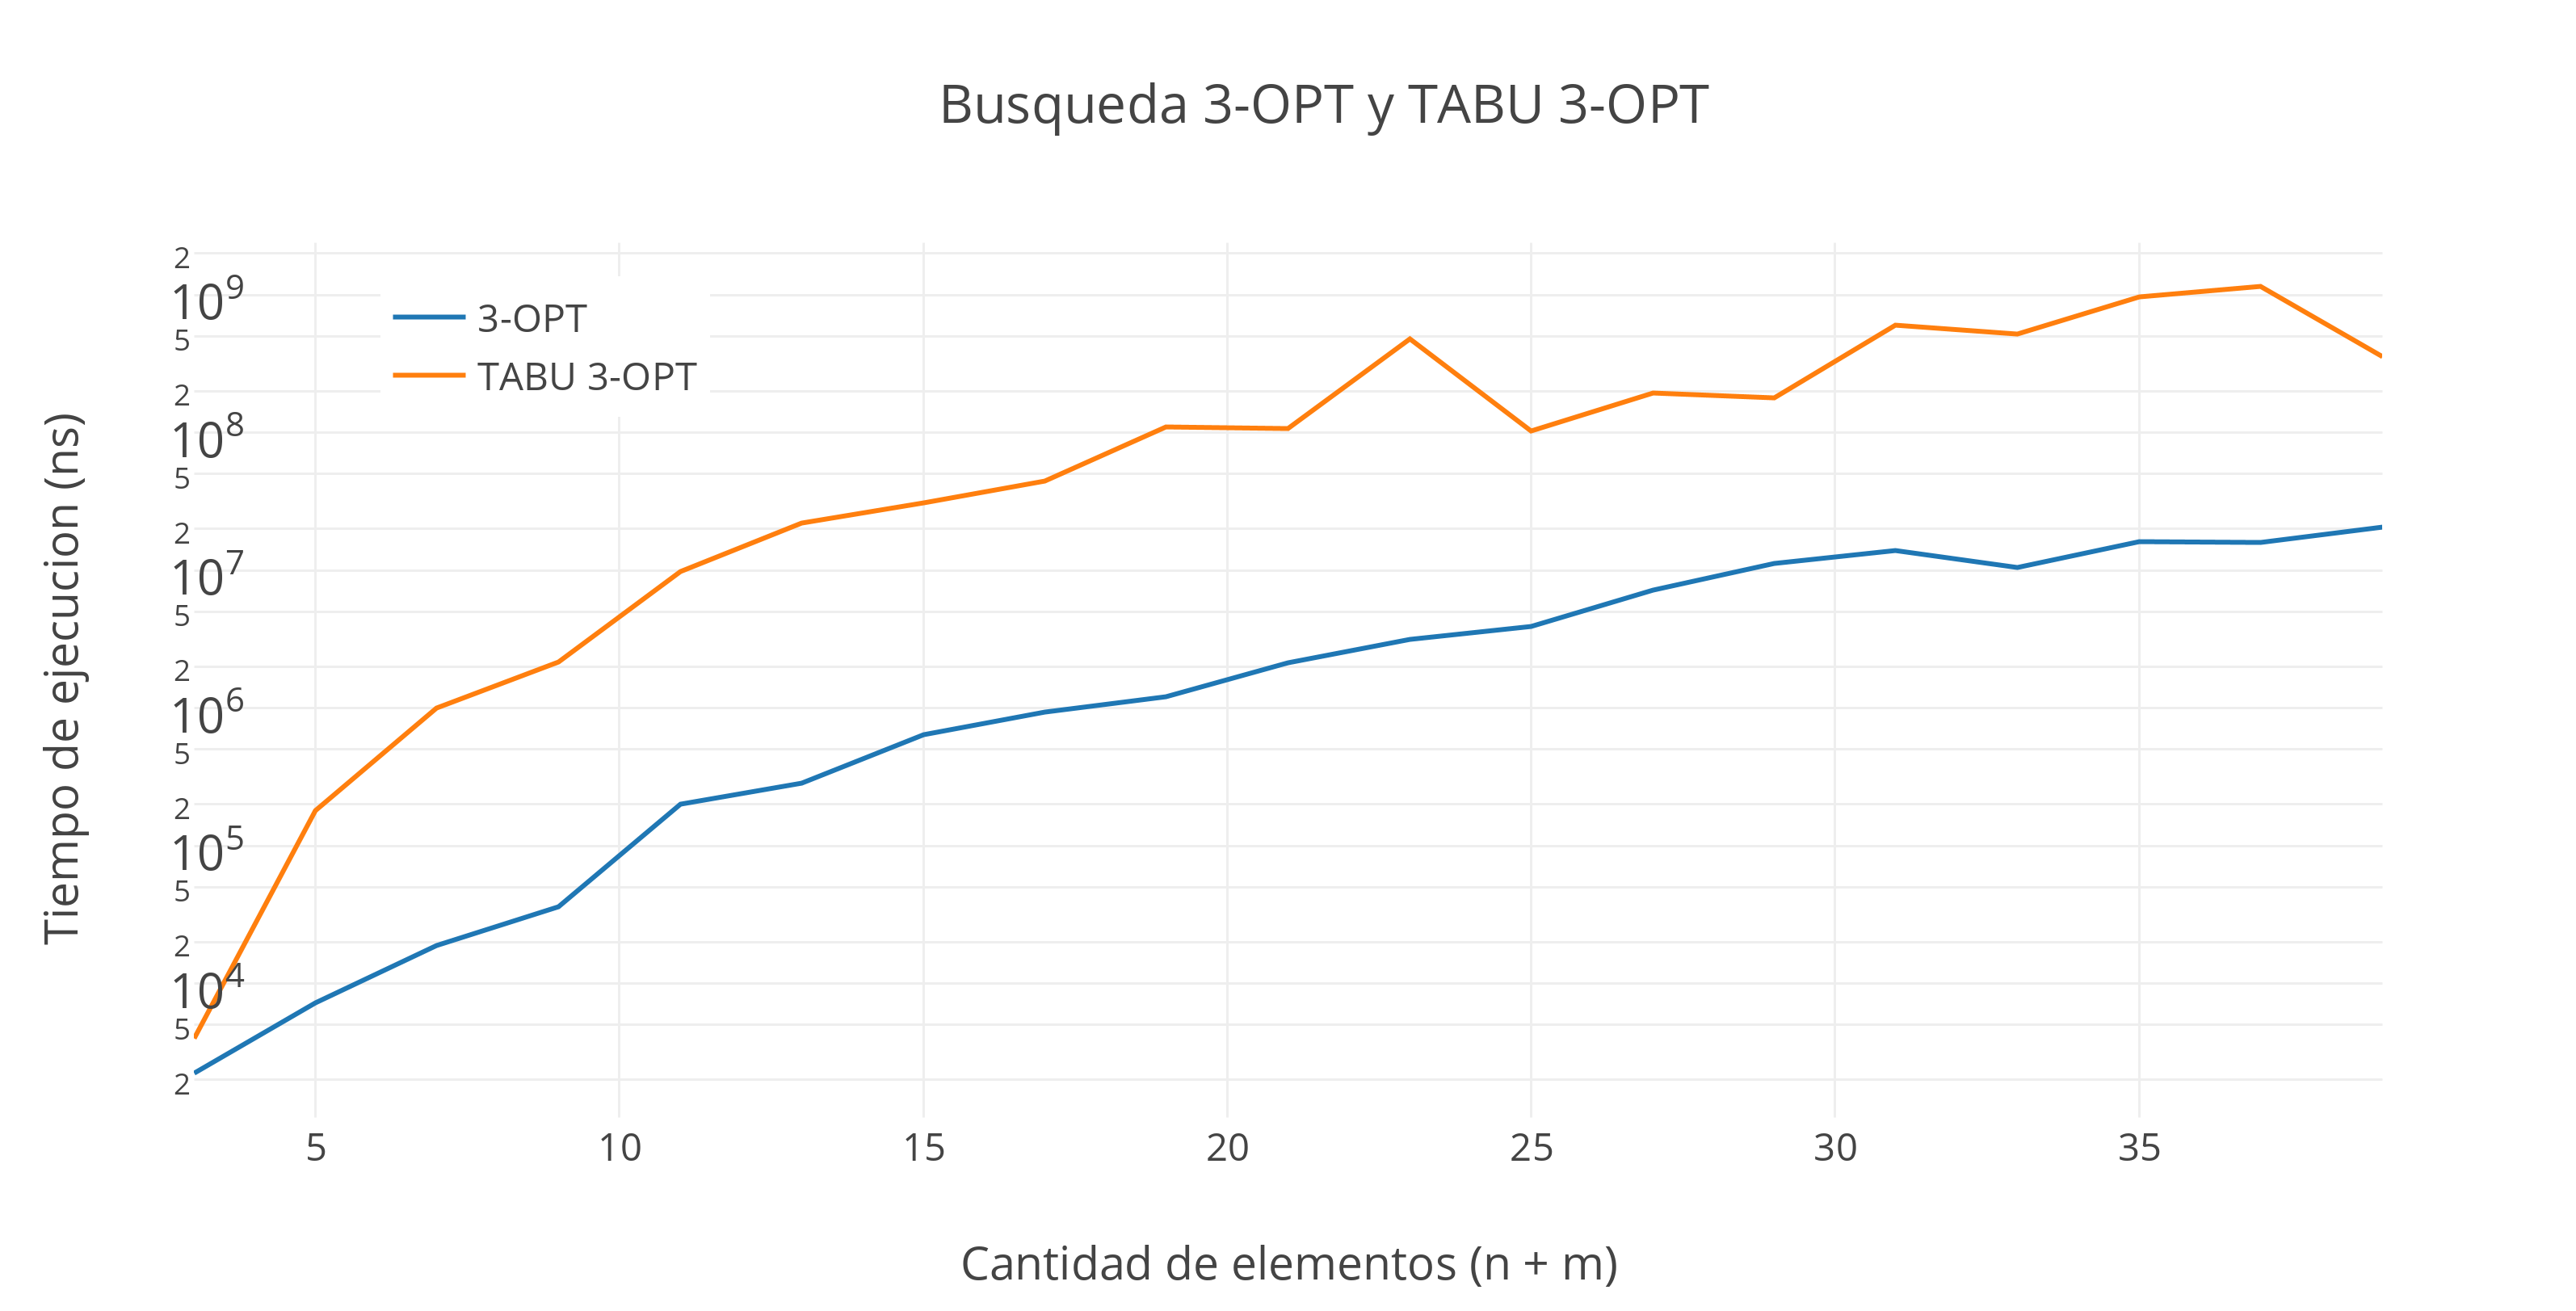
\includegraphics[scale=0.5]{./EJ4/medicion3optgym0.png}\\
 {            \textit{Gráfico \ 4.4 - 3-OPT vs Tabu 3-OPT sobre Familia 4}}
  \end{center}
  \vspace*{0.3cm}
  
Podemos observar que tabú search 2-OPT mejora lo realizado por la heuristica de búsqueda local 2-OPT. Los tiempos insumidos para lograrlo son elevados, pero en relación a la mejora es un resultado aceptable en la práctica. No así tabú search 3-OPT que apenas mejora lo realizado por búsqueda local 3-OPT y requiere tiempos elevados de corrida del algoritmo.\\
  
Para decidir que vecindad es mejor utilizar en tabú search, se comparará conjuntamente el tiempo de ejecución con la calidad de la solución. Para esta última tendremos en cuenta que los algoritmos, de devolver un resultado, serán válidos: esto quiere decir que cuanto menor distancia recorran las soluciones, mejor serán las mismas:

Las soluciones obtenidas fueron las siguientes:

\vspace*{0.3cm} \vspace*{0.3cm}
  \begin{center}
 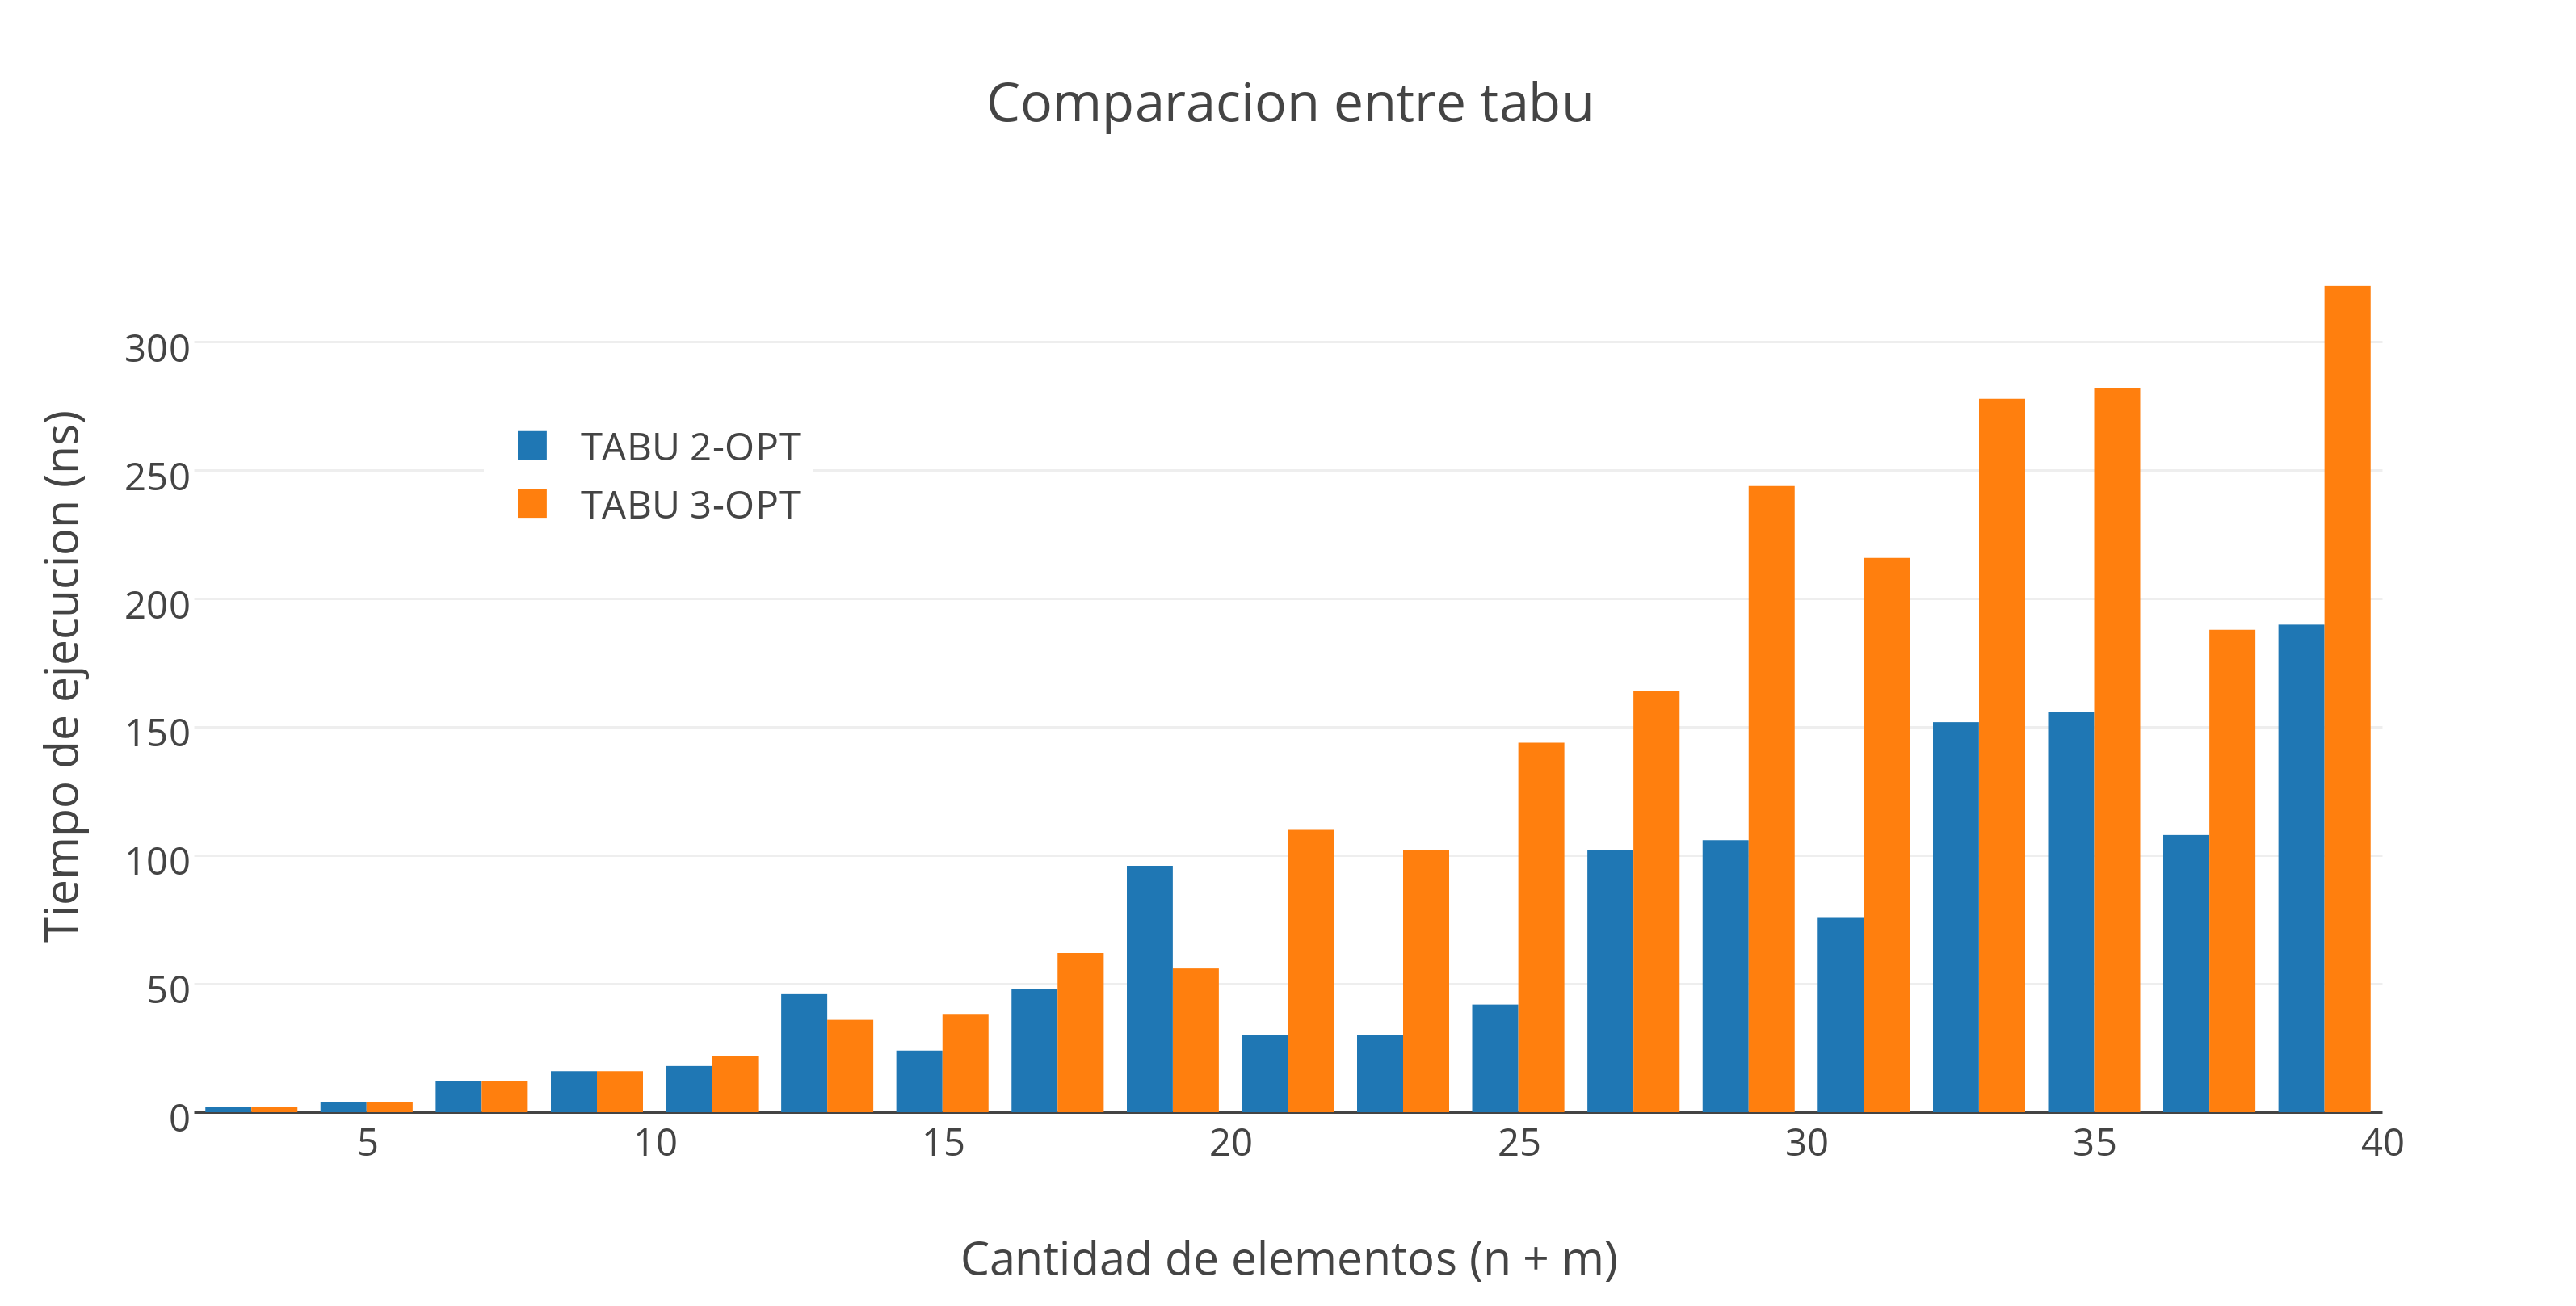
\includegraphics[scale=0.5]{./EJ4/comparativogym0.png}\\
 {            \textit{Gráfico \ 4.5 - Tabu 2-OPT vs Tabu 3-OPT sobre Familia 4}}
  \end{center}
  \vspace*{0.3cm}

En cuanto a tiempo insumido vemos lo siguiente:

\vspace*{0.3cm} \vspace*{0.3cm}
  \begin{center}
 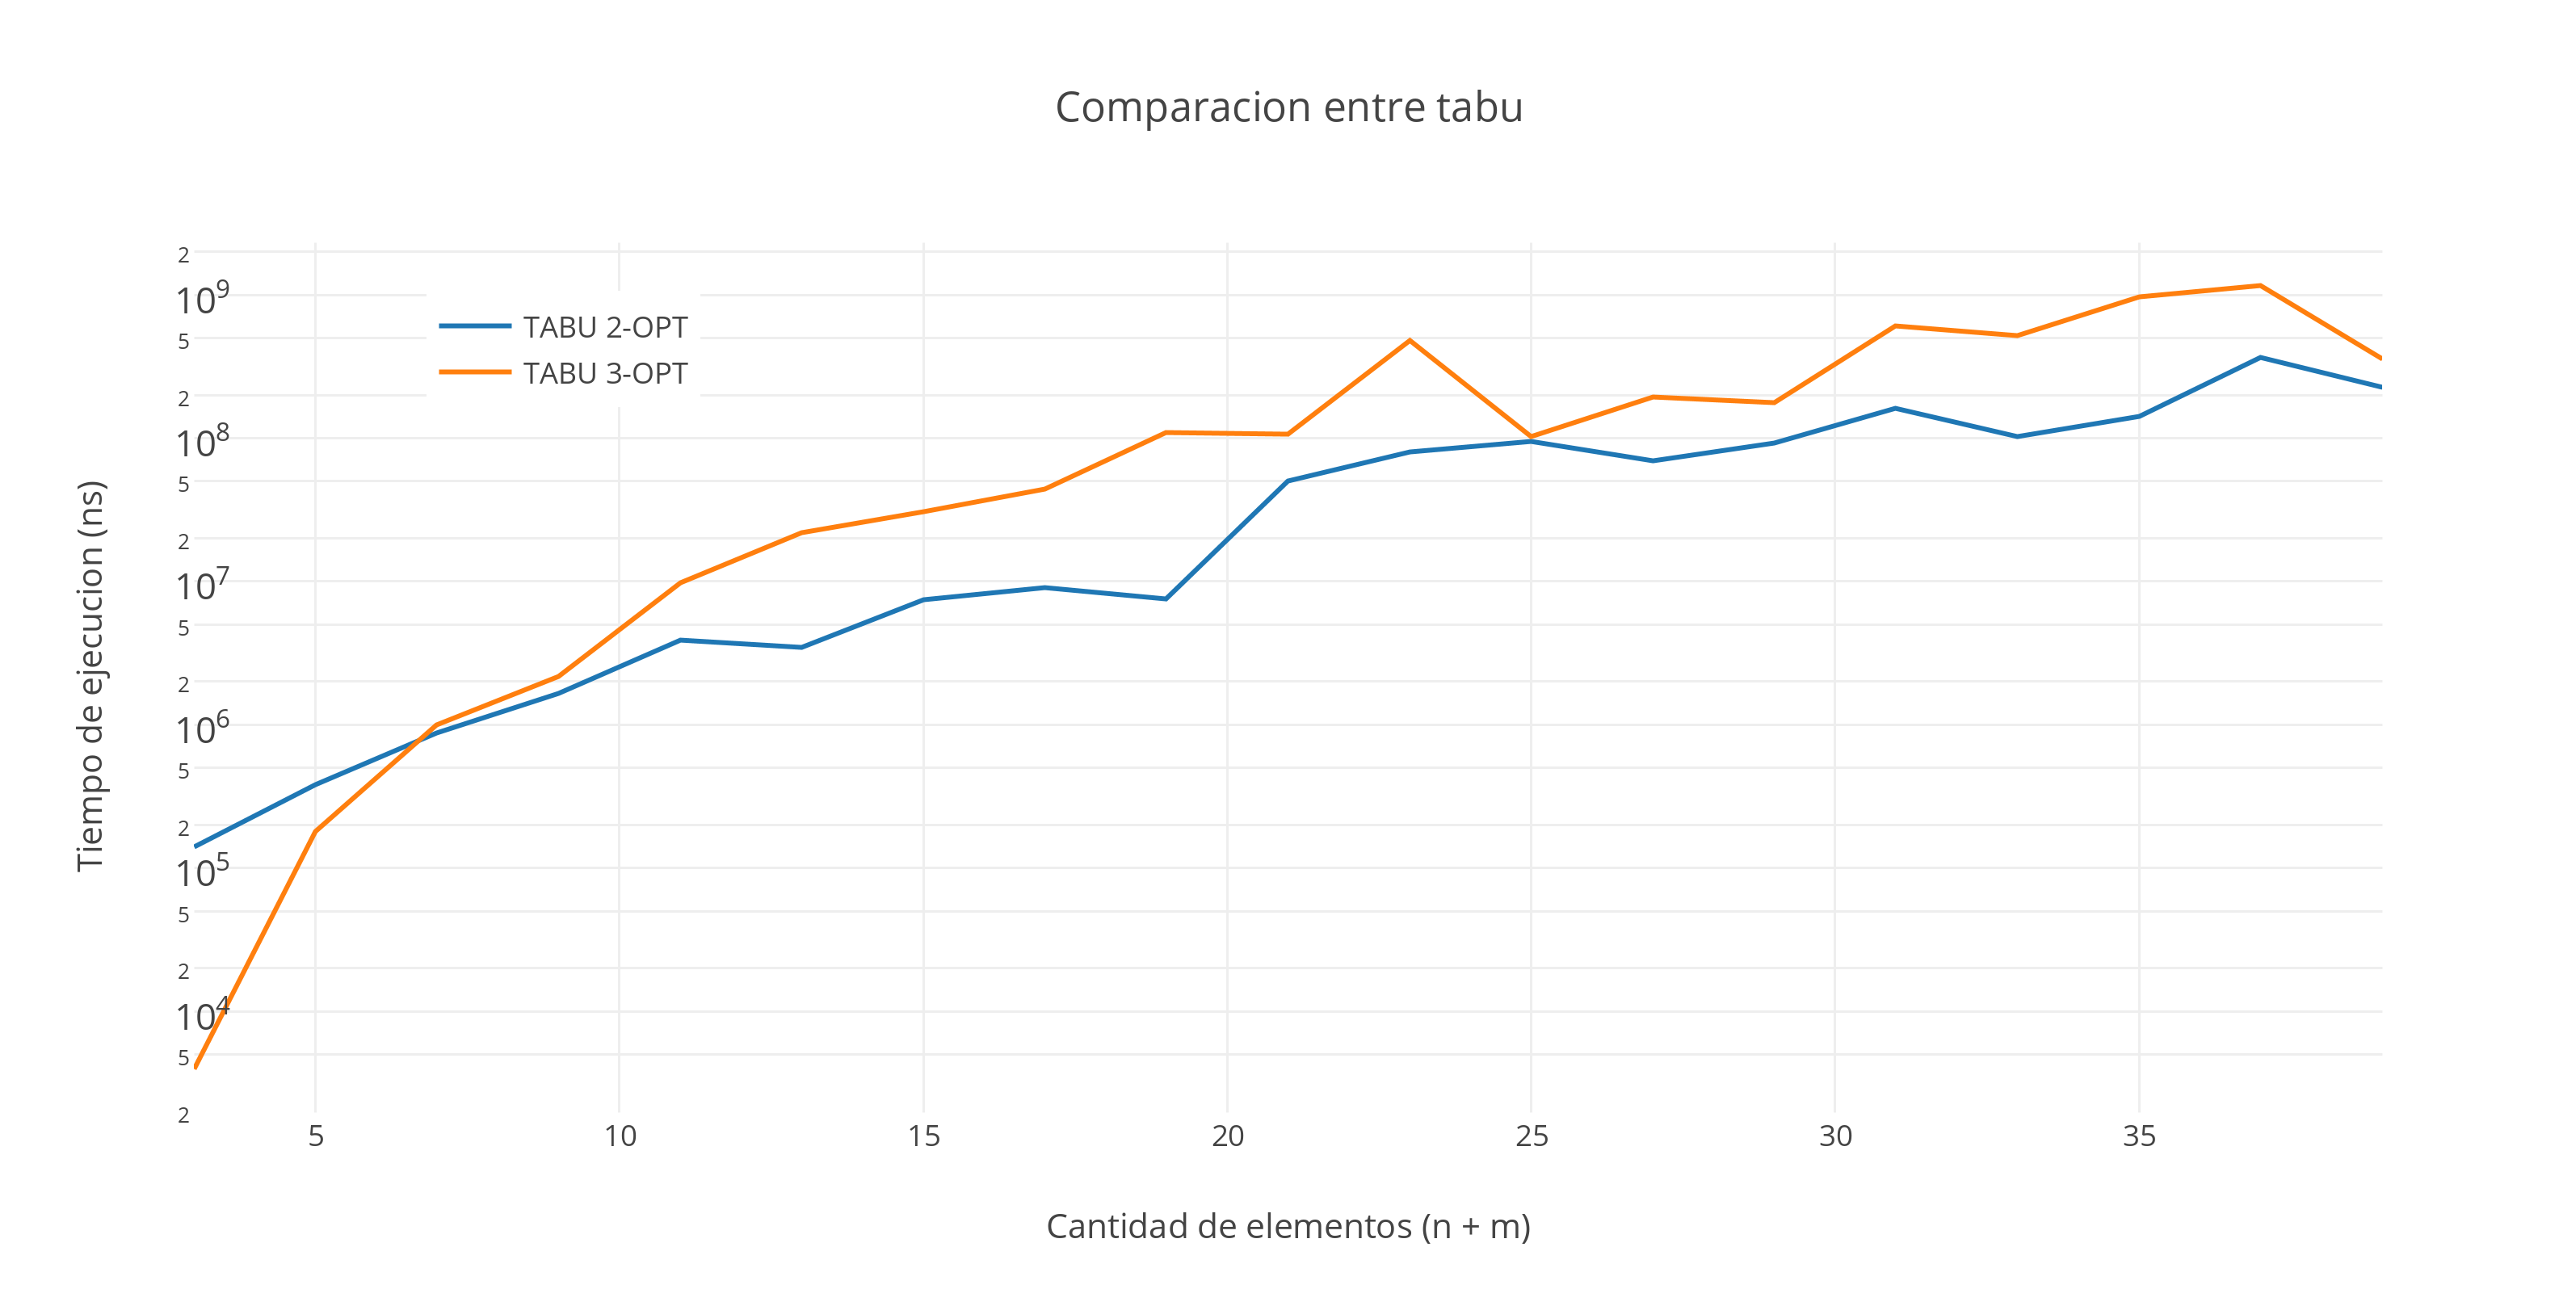
\includegraphics[scale=0.5]{./EJ4/comparaciongym01.png}\\
 {            \textit{Gráfico \ 4.6 - Tabu 2-OPT vs Tabu 3-OPT sobre Familia 4}}
  \end{center}
  \vspace*{0.3cm}

--> OBTENER CONCLUSIONES

\subsubsection*{Familia 6}

--> PRESENTAR FAMILIA

\vspace*{0.3cm} \vspace*{0.3cm}
  \begin{center}
 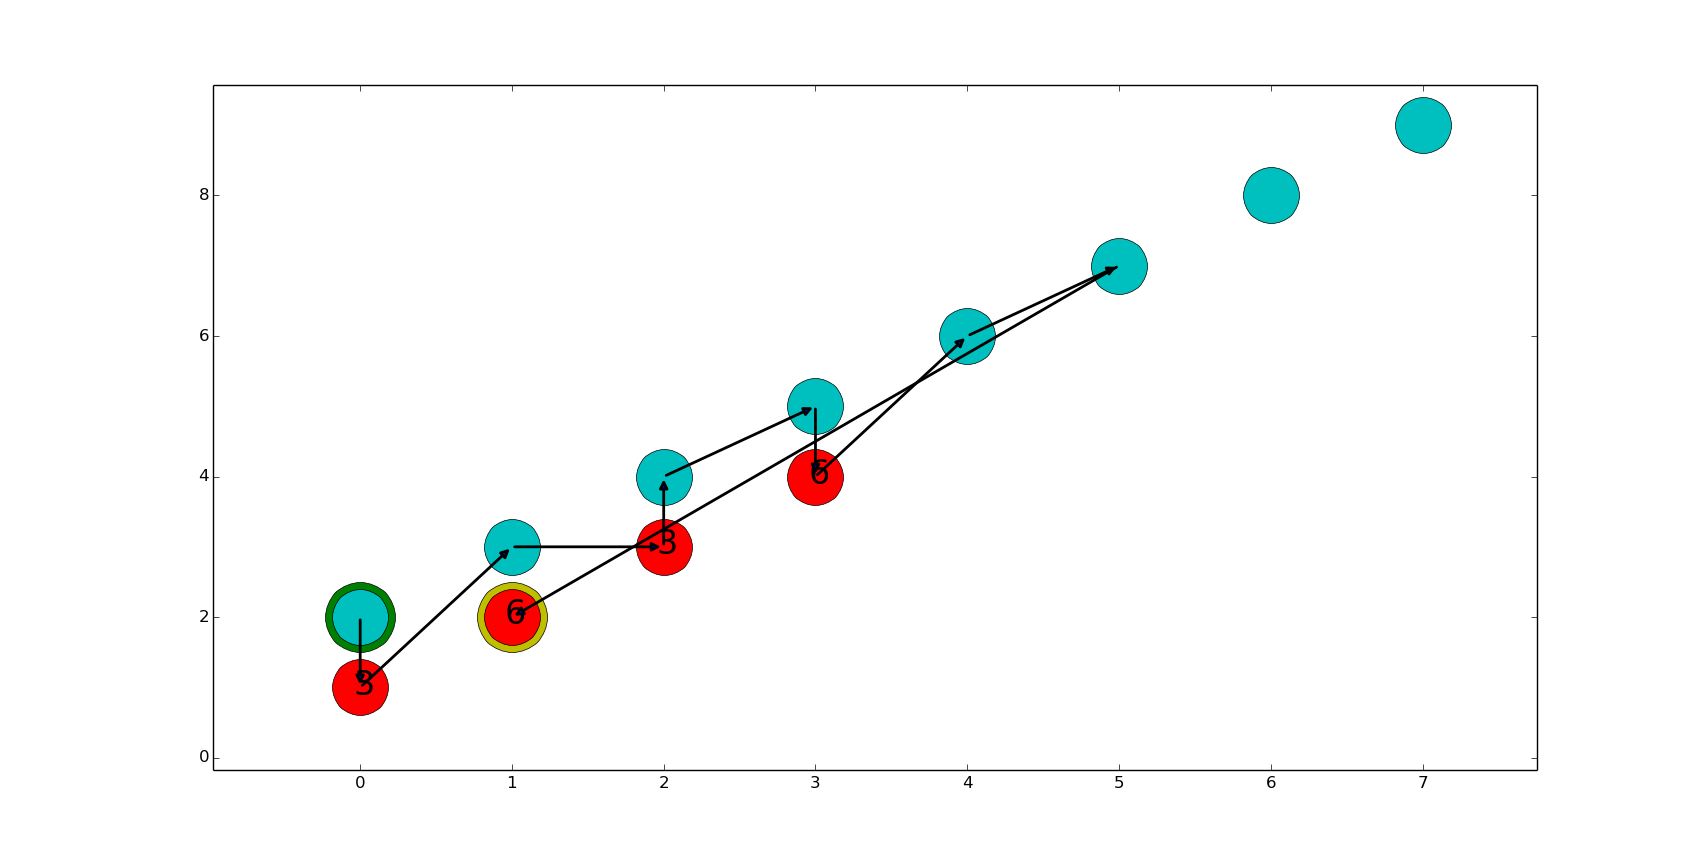
\includegraphics[scale=0.3]{./EJ4/fam6goloso.png}\\
 {            \textit{Soluci\'on Golosa}}
  \end{center}
  \vspace*{0.3cm}

\vspace*{0.3cm} \vspace*{0.3cm}
  \begin{center}
 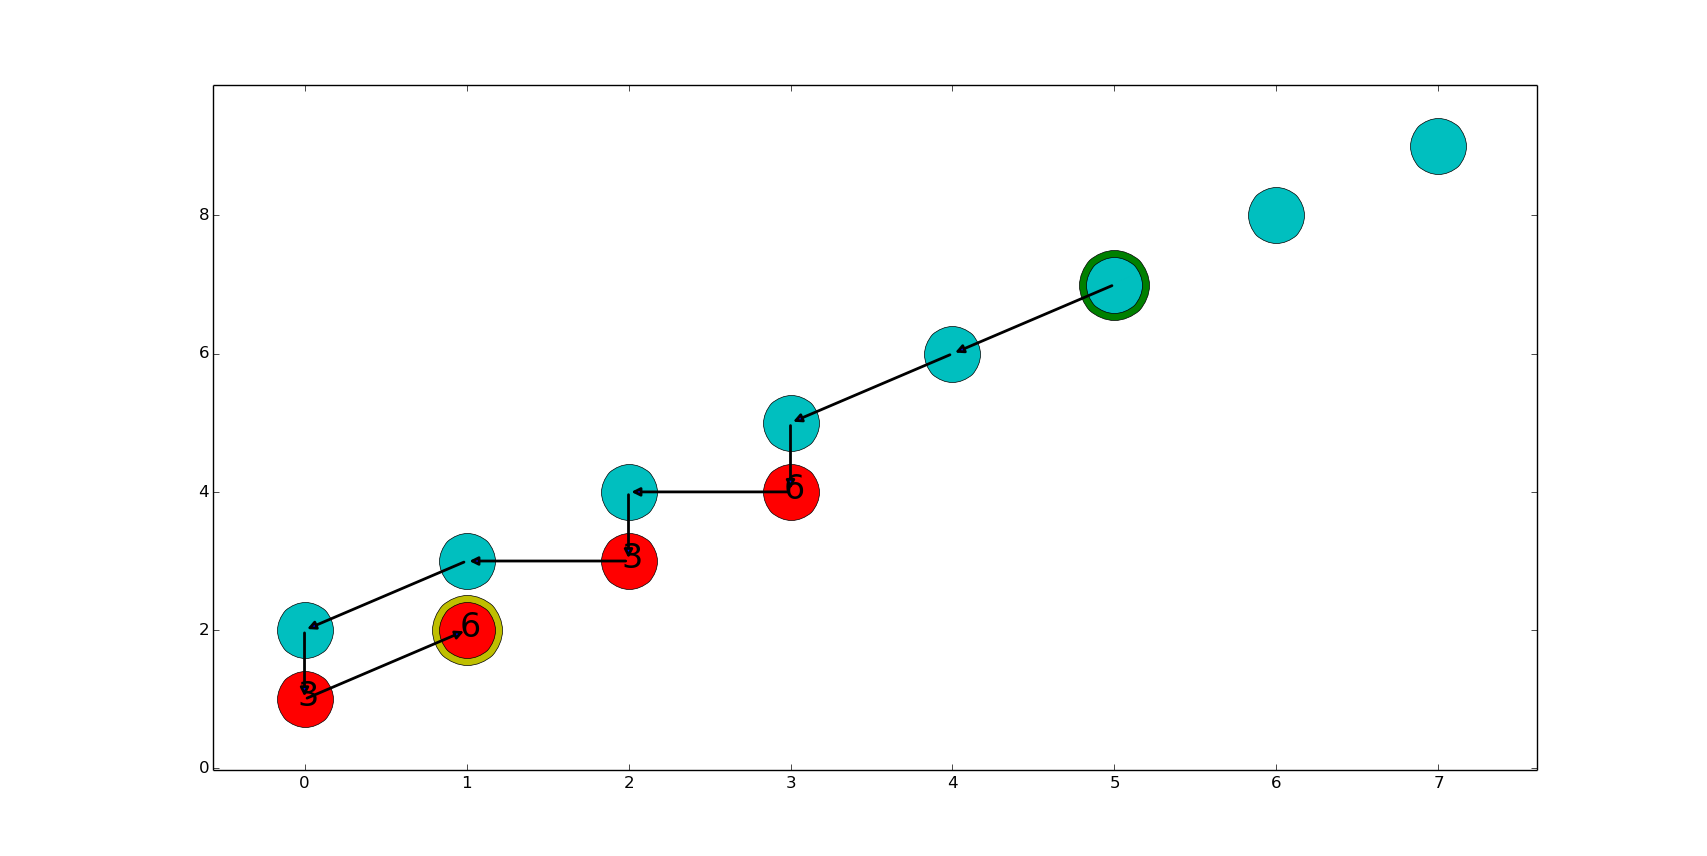
\includegraphics[scale=0.3]{./EJ4/fam62opt.png}\\
 {            \textit{Soluci\'on TABU 2-OPT}}
  \end{center}
  \vspace*{0.3cm}

\vspace*{0.3cm} \vspace*{0.3cm}
  \begin{center}
 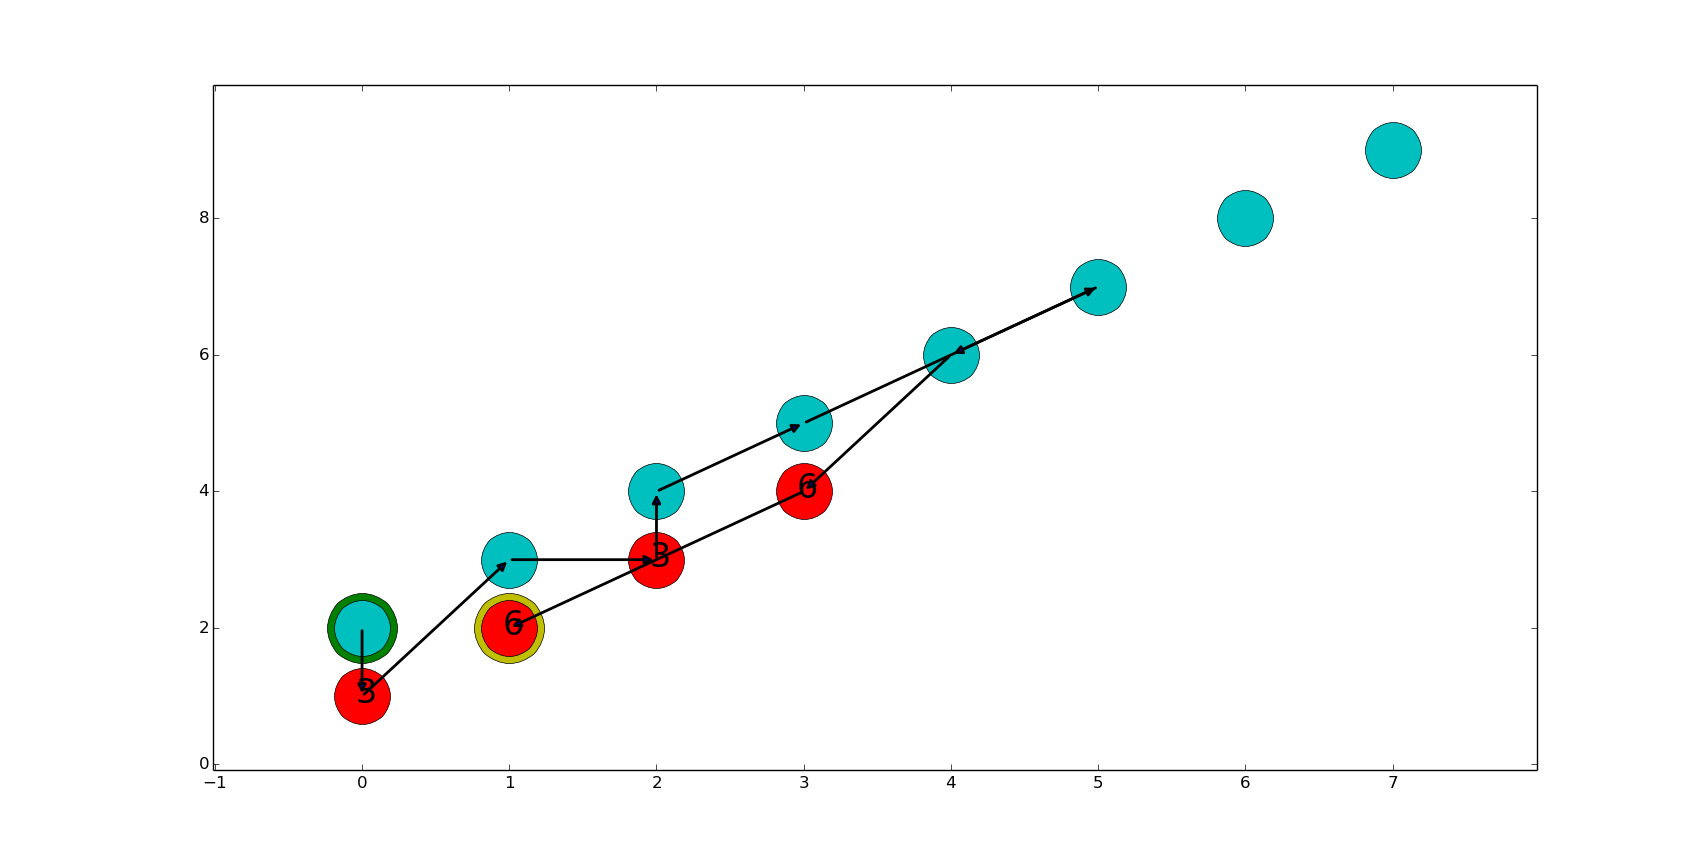
\includegraphics[scale=0.3]{./EJ4/fam63opt.png}\\
 {            \textit{Soluci\'on TABU 3-OPT}}
  \end{center}
  \vspace*{0.3cm}

Veamos como se comporta Tabu 2-OPT con respecto a la heuristica de busqueda local 2-OPT:

\vspace*{0.3cm} \vspace*{0.3cm}
  \begin{center}
 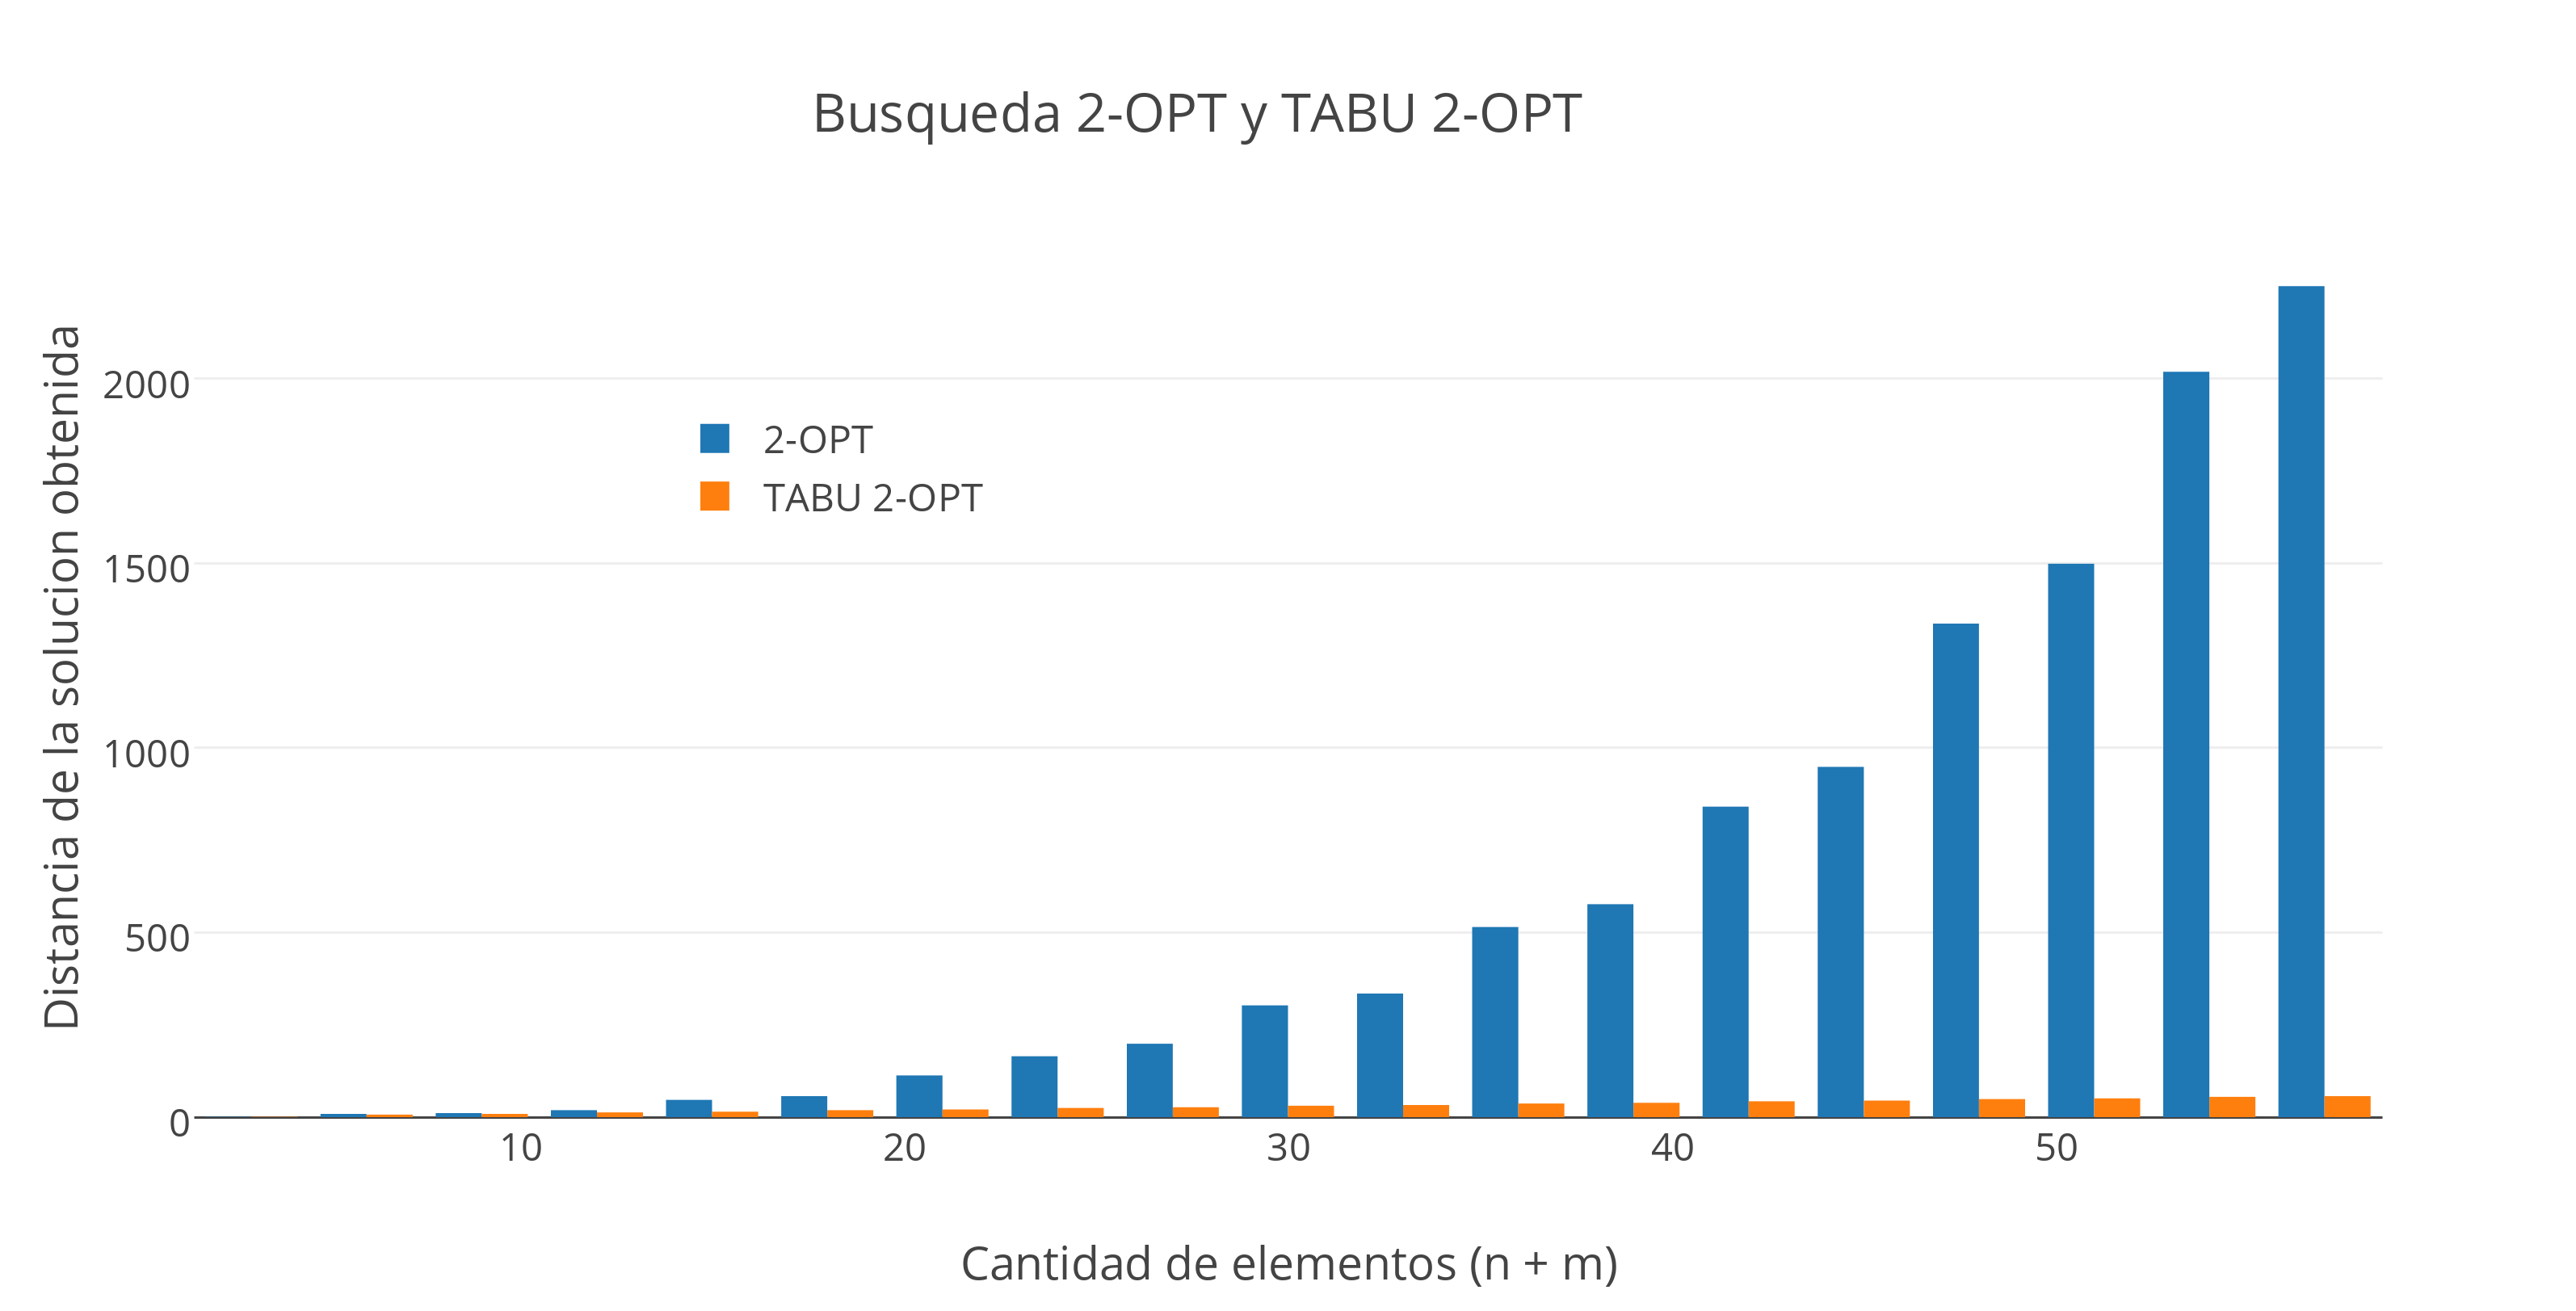
\includegraphics[scale=0.5]{./EJ4/comparativosinorden2opt.png}\\
 {            \textit{Gráfico \ 4.7 - 2-OPT vs Tabu 2-OPT sobre Familia 6}}
  \end{center}
  \vspace*{0.3cm}

\vspace*{0.3cm} \vspace*{0.3cm}
  \begin{center}
 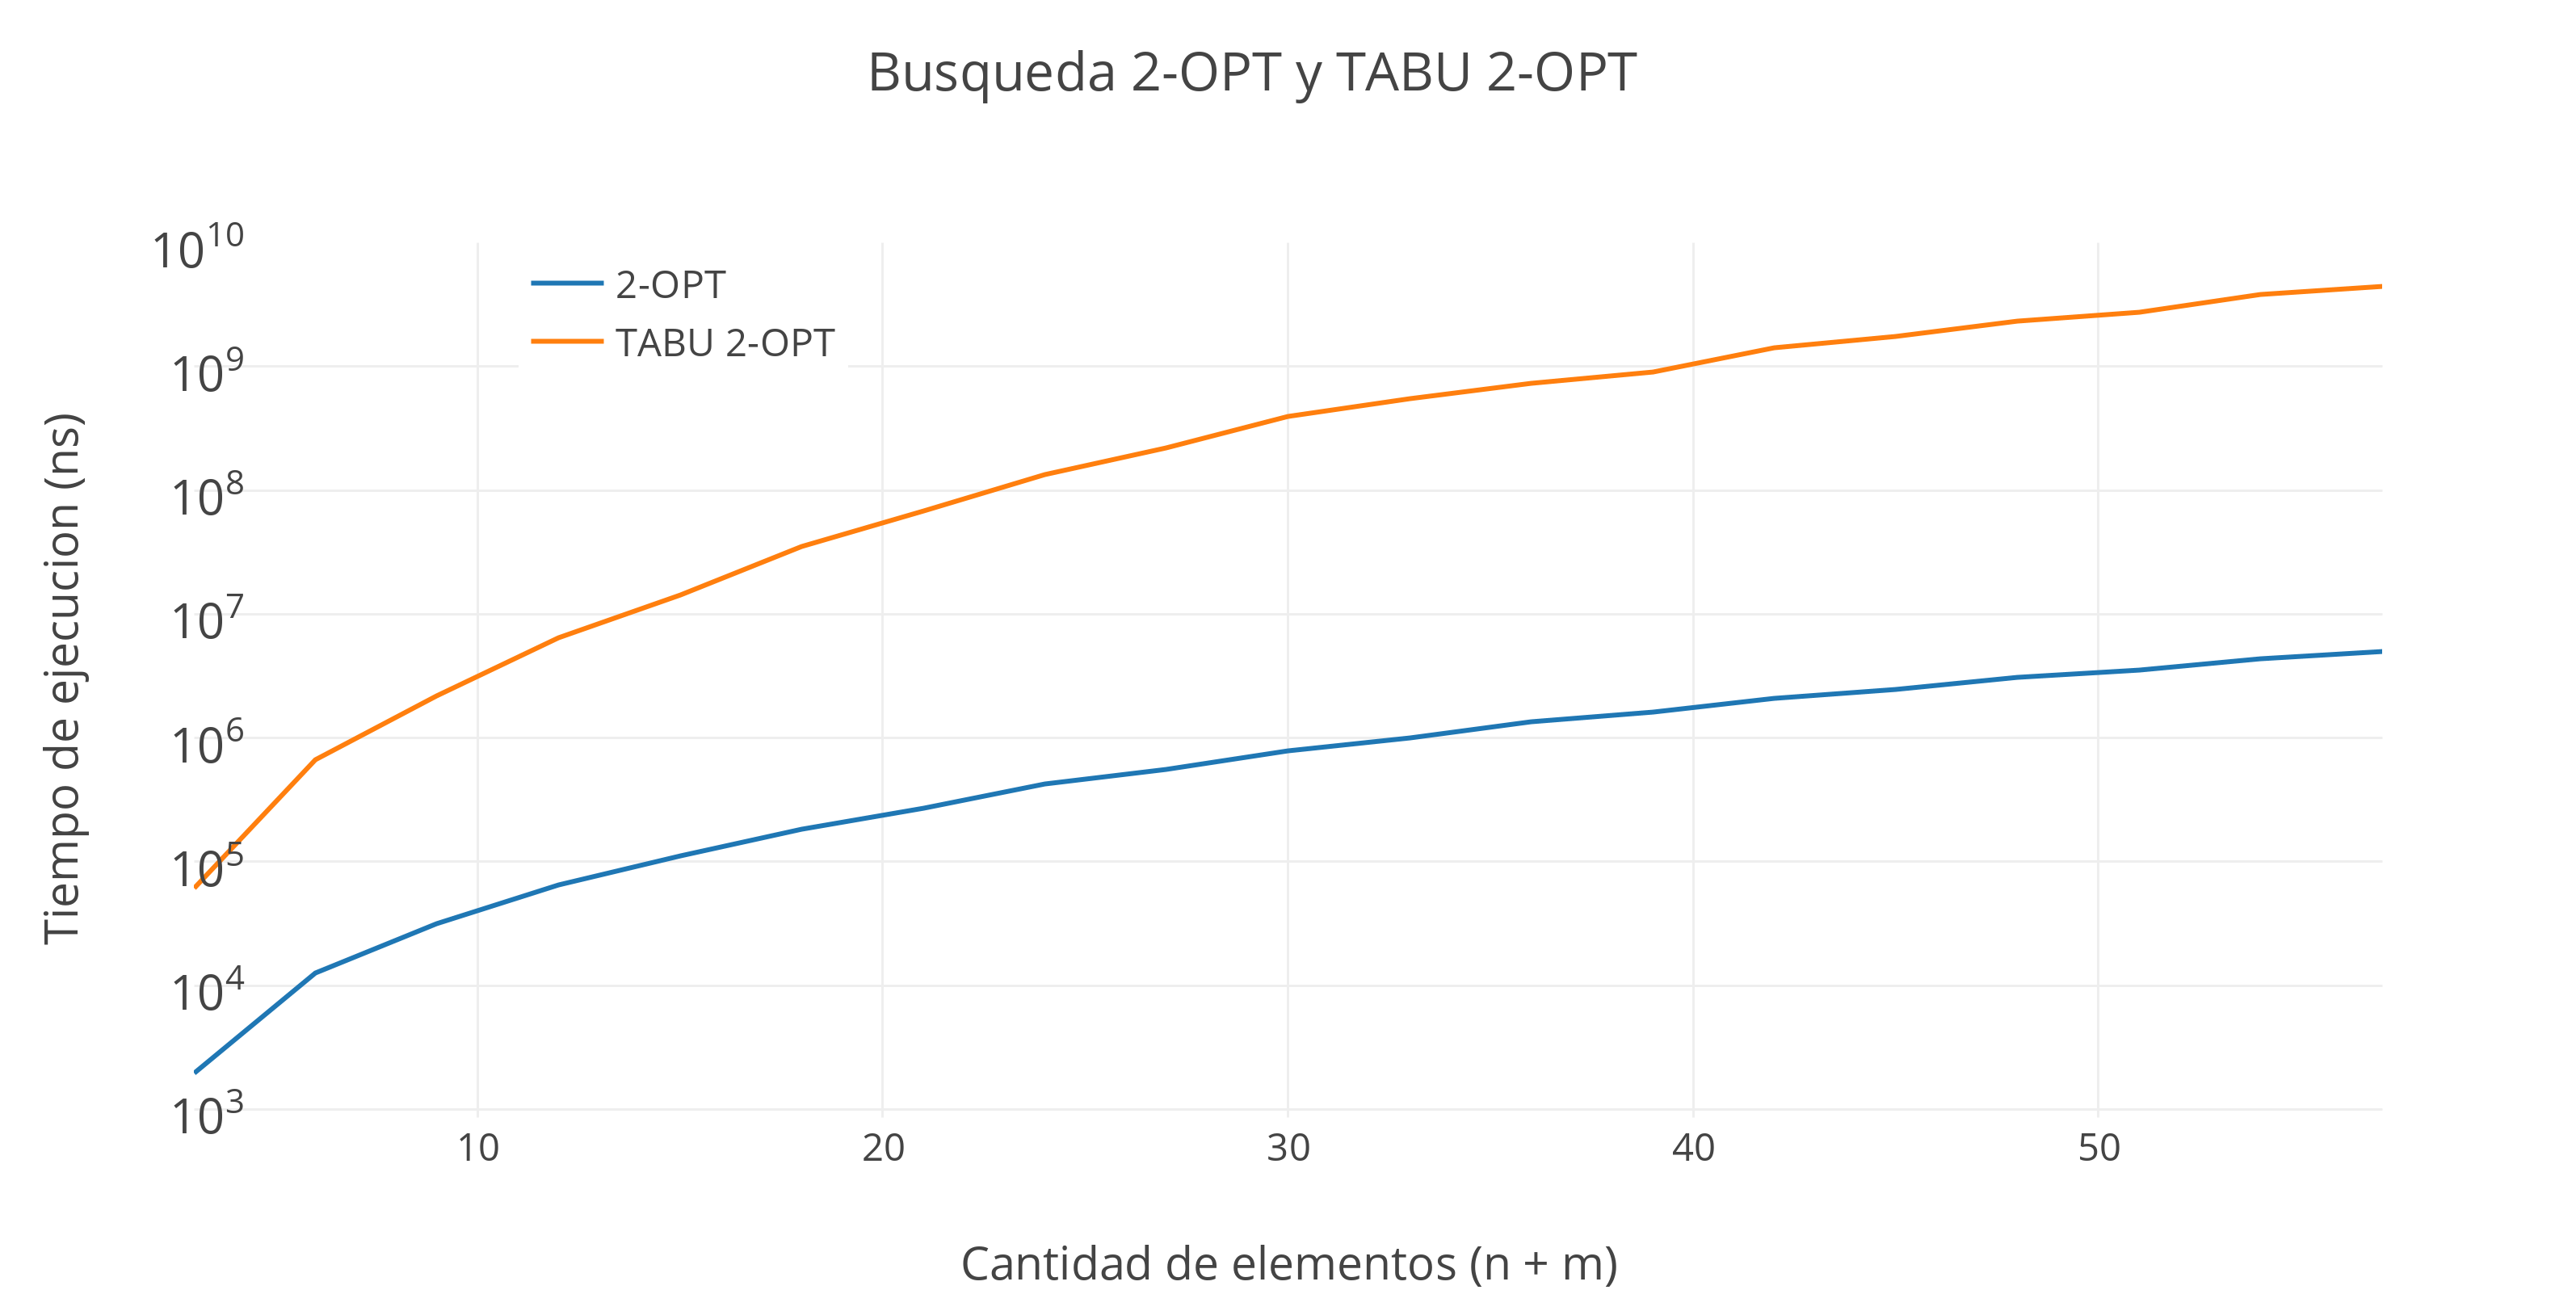
\includegraphics[scale=0.5]{./EJ4/medicion2optsinorden.png}\\
 {            \textit{Gráfico \ 4.8 - 2-OPT vs Tabu 2-OPT sobre Familia 6}}
  \end{center}
  \vspace*{0.3cm}

Luego, para 3-OPT:

\vspace*{0.3cm} \vspace*{0.3cm}
  \begin{center}
 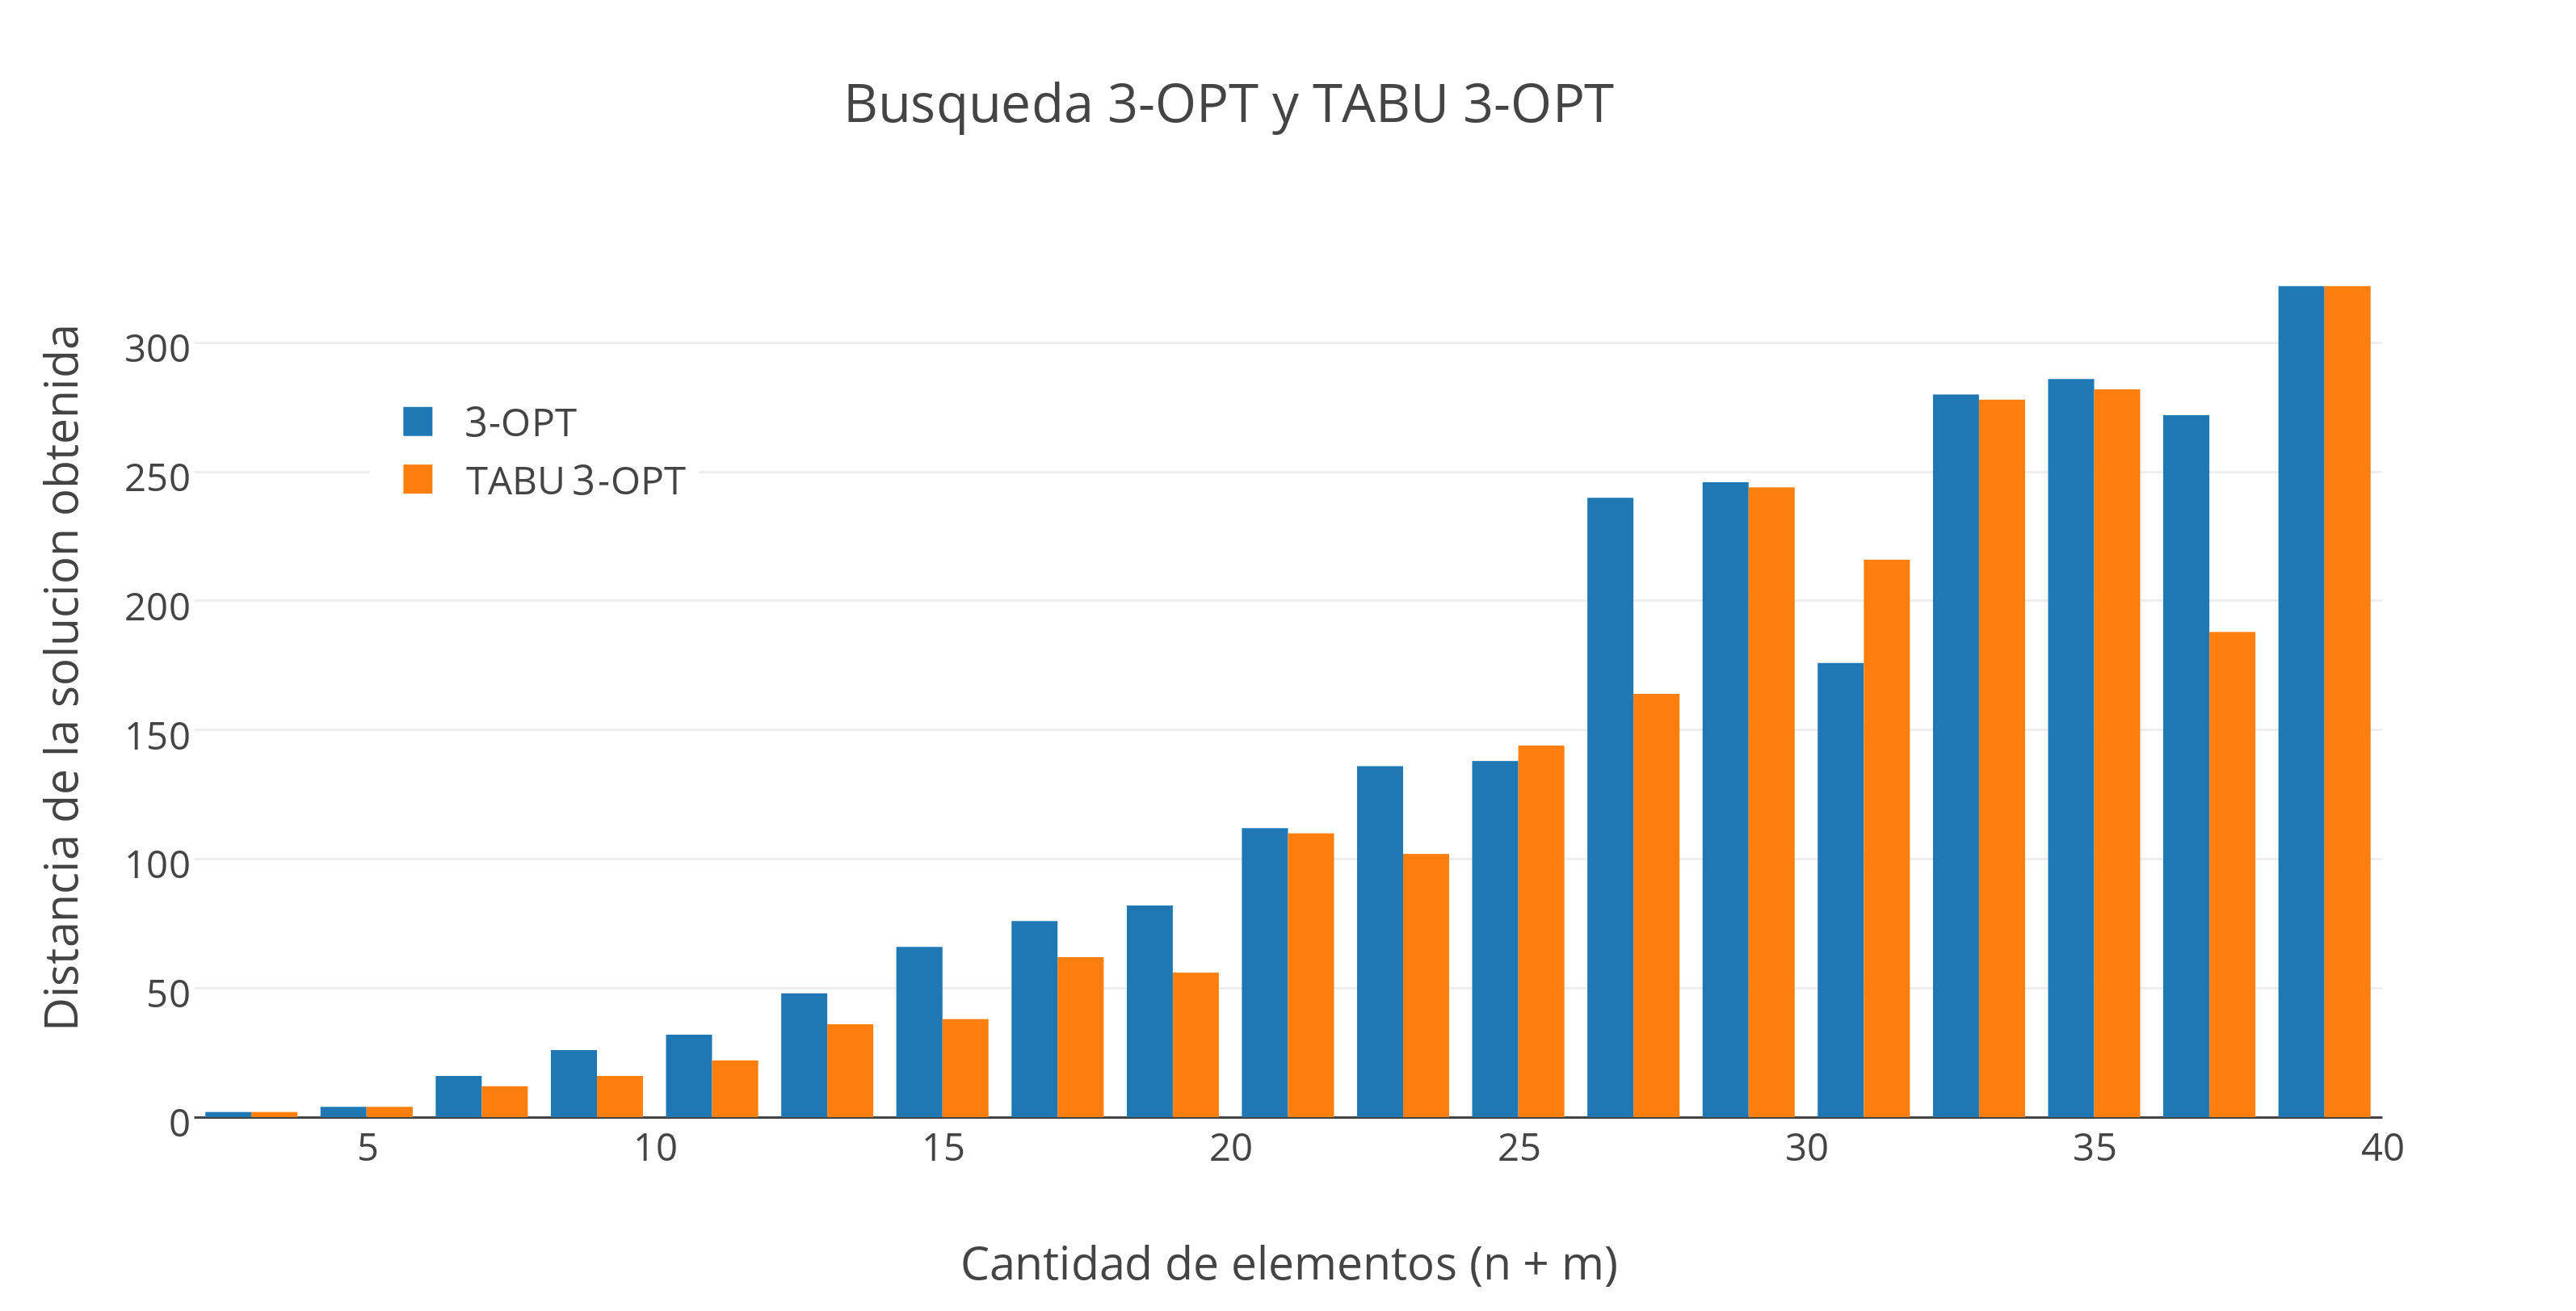
\includegraphics[scale=0.5]{./EJ4/comparativogym03opt.png}\\
 {            \textit{Gráfico \ 4.9 - 3-OPT vs Tabu 3-OPT sobre Familia 6}}
  \end{center}
  \vspace*{0.3cm}

\vspace*{0.3cm} \vspace*{0.3cm}
  \begin{center}
 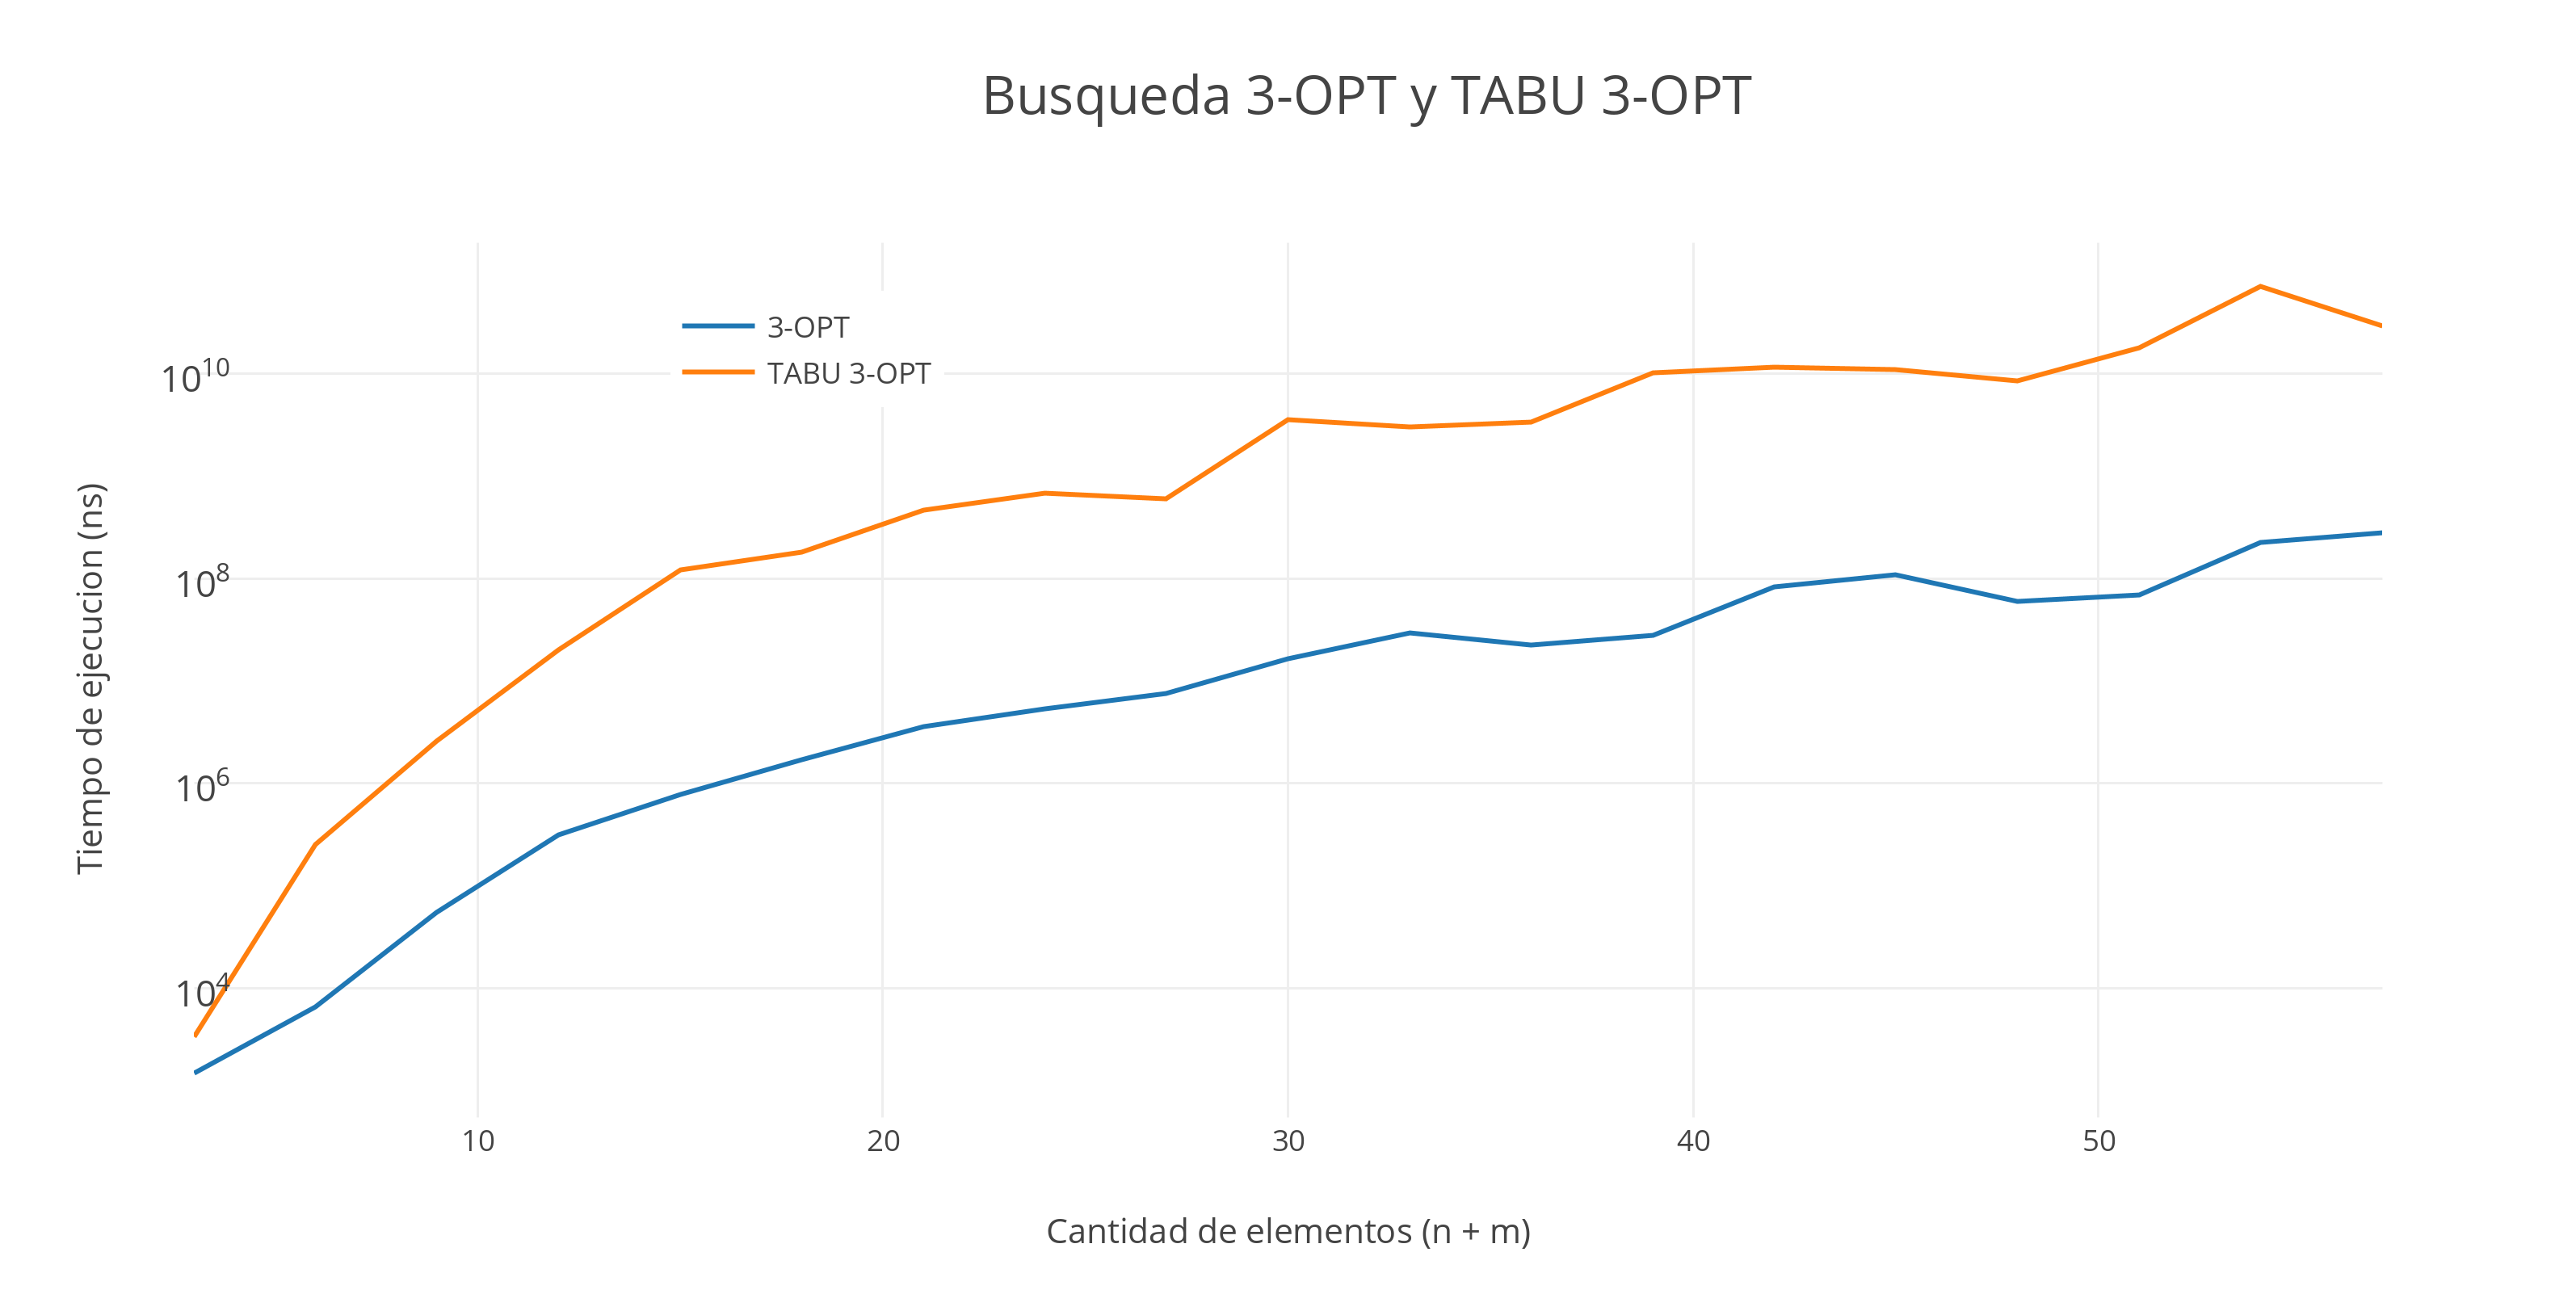
\includegraphics[scale=0.5]{./EJ4/medicion3optsinorden.png}\\
 {            \textit{Gráfico \ 4.10 - 3-OPT vs Tabu 3-OPT sobre Familia 6}}
  \end{center}
  \vspace*{0.3cm}
  
--> OBTENER CONCLUSIONES
  
Comparando las soluciones de cada version de tabú search podemos observar lo siguiente:

\vspace*{0.3cm} \vspace*{0.3cm}
  \begin{center}
 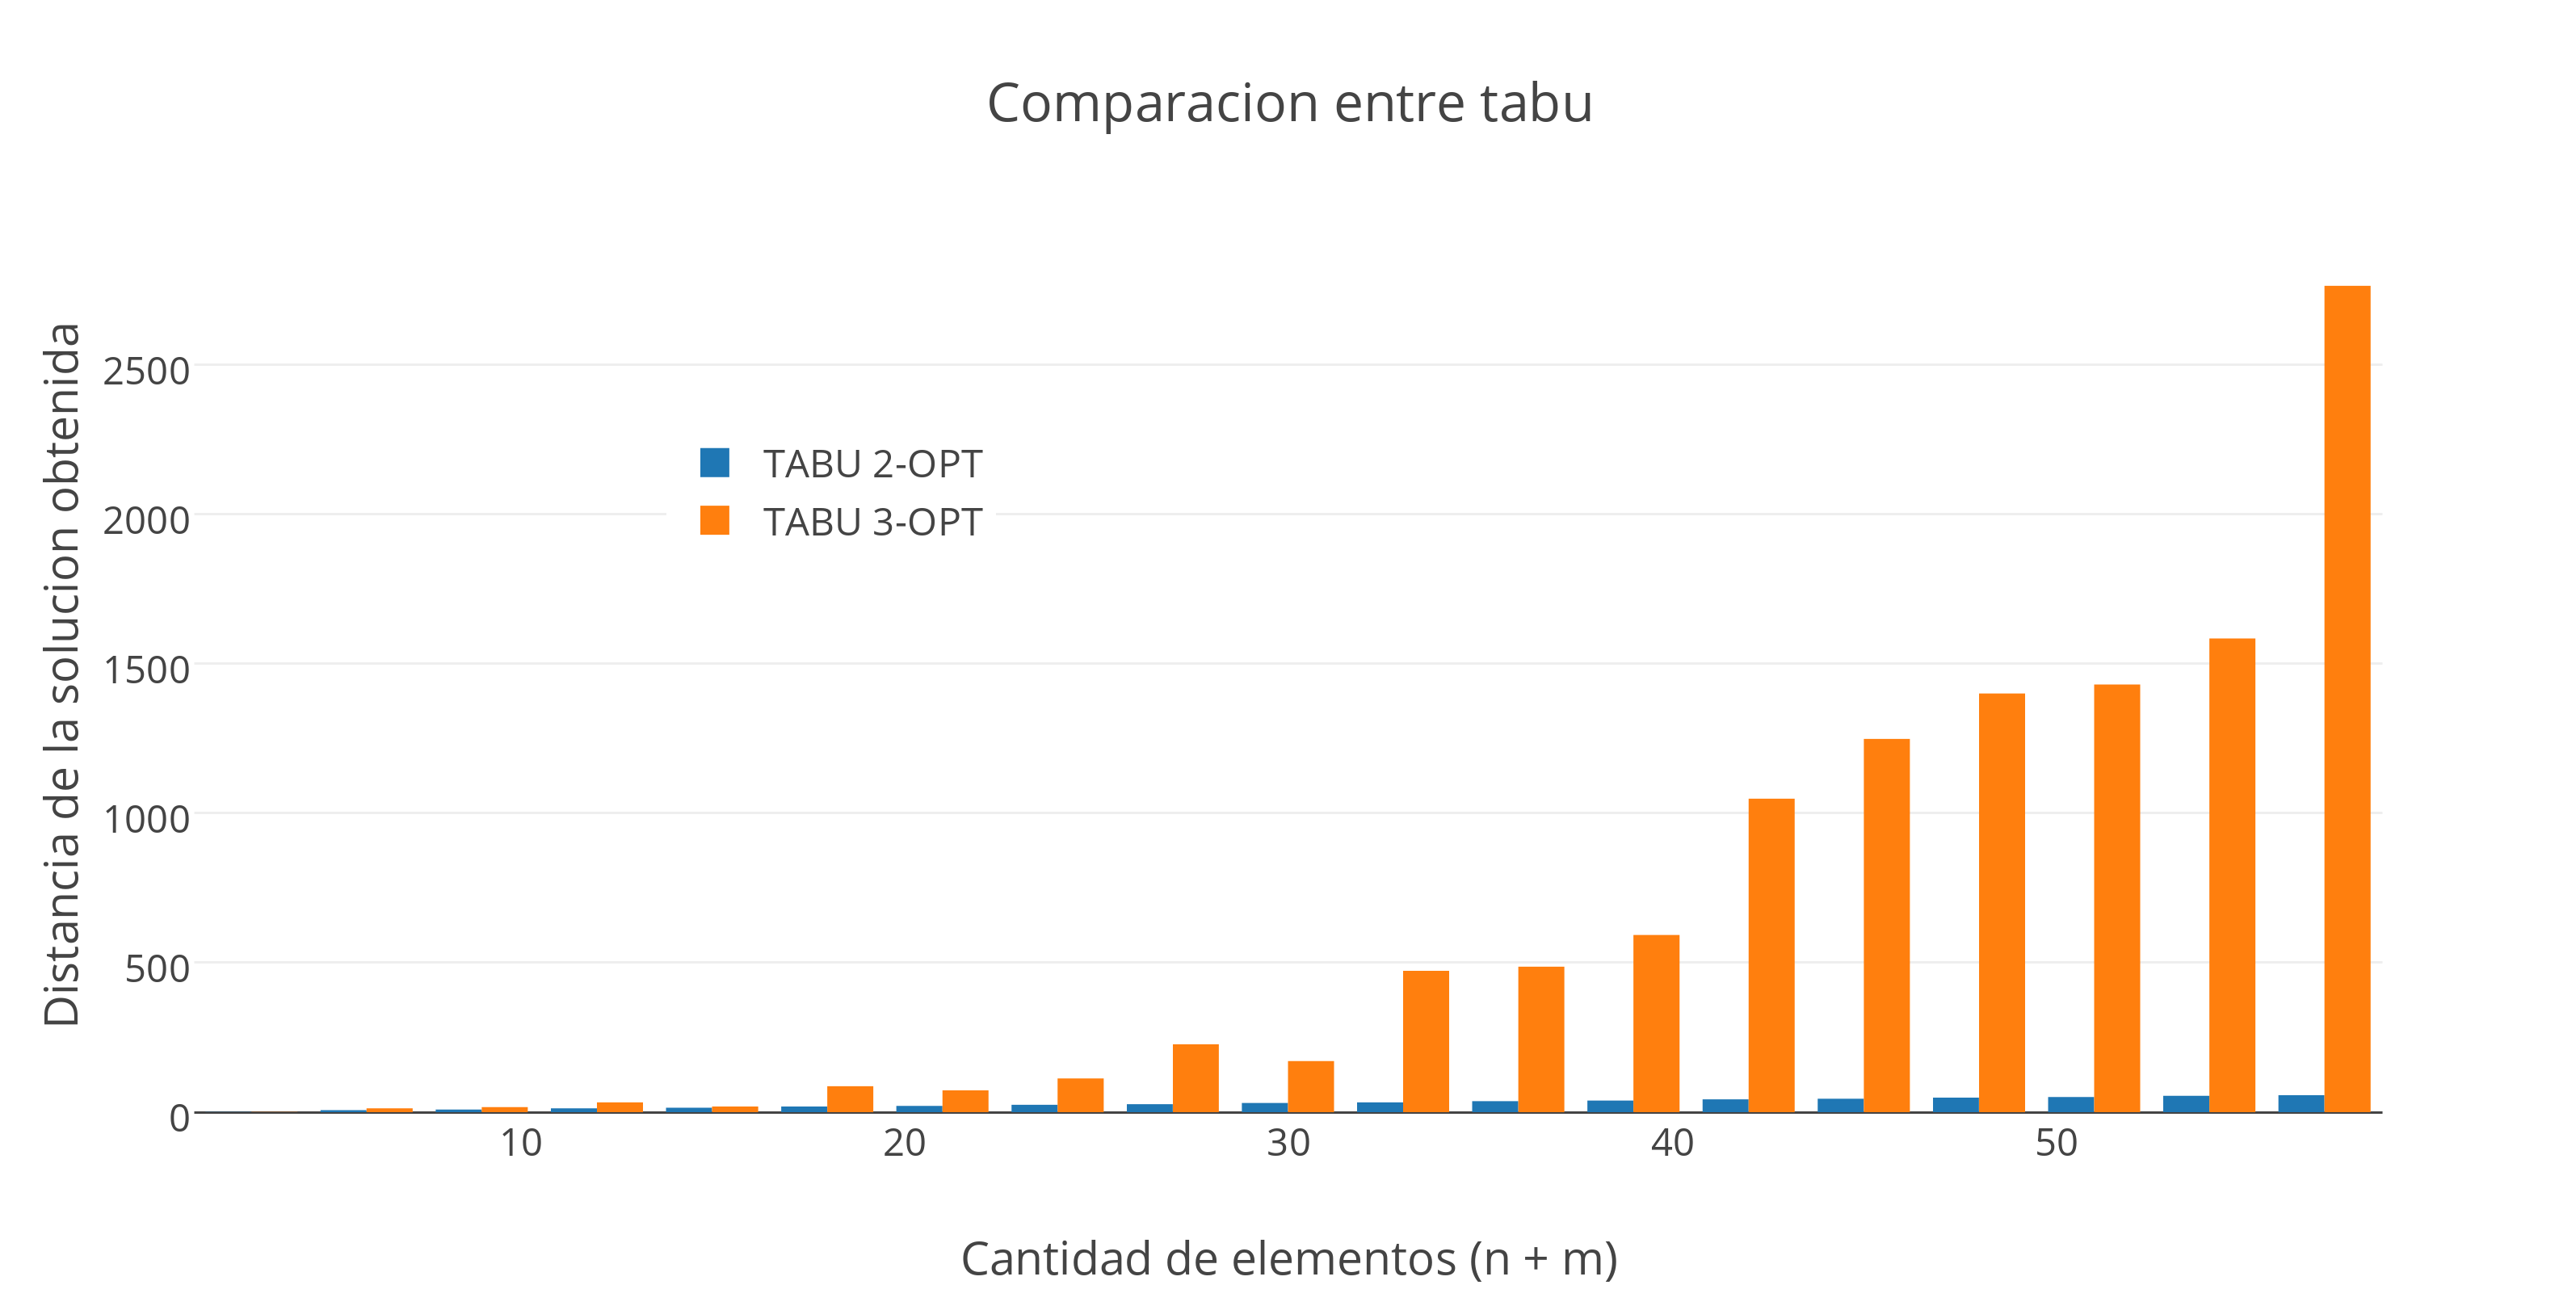
\includegraphics[scale=0.5]{./EJ4/comparativosinorden.png}\\
 {            \textit{Gráfico \ 4.11 - Tabu 2-OPT vs Tabu 3-OPT sobre Familia 6}}
  \end{center}
  \vspace*{0.3cm}

En cuanto a tiempo insumido vemos lo siguiente:

\vspace*{0.3cm} \vspace*{0.3cm}
  \begin{center}
 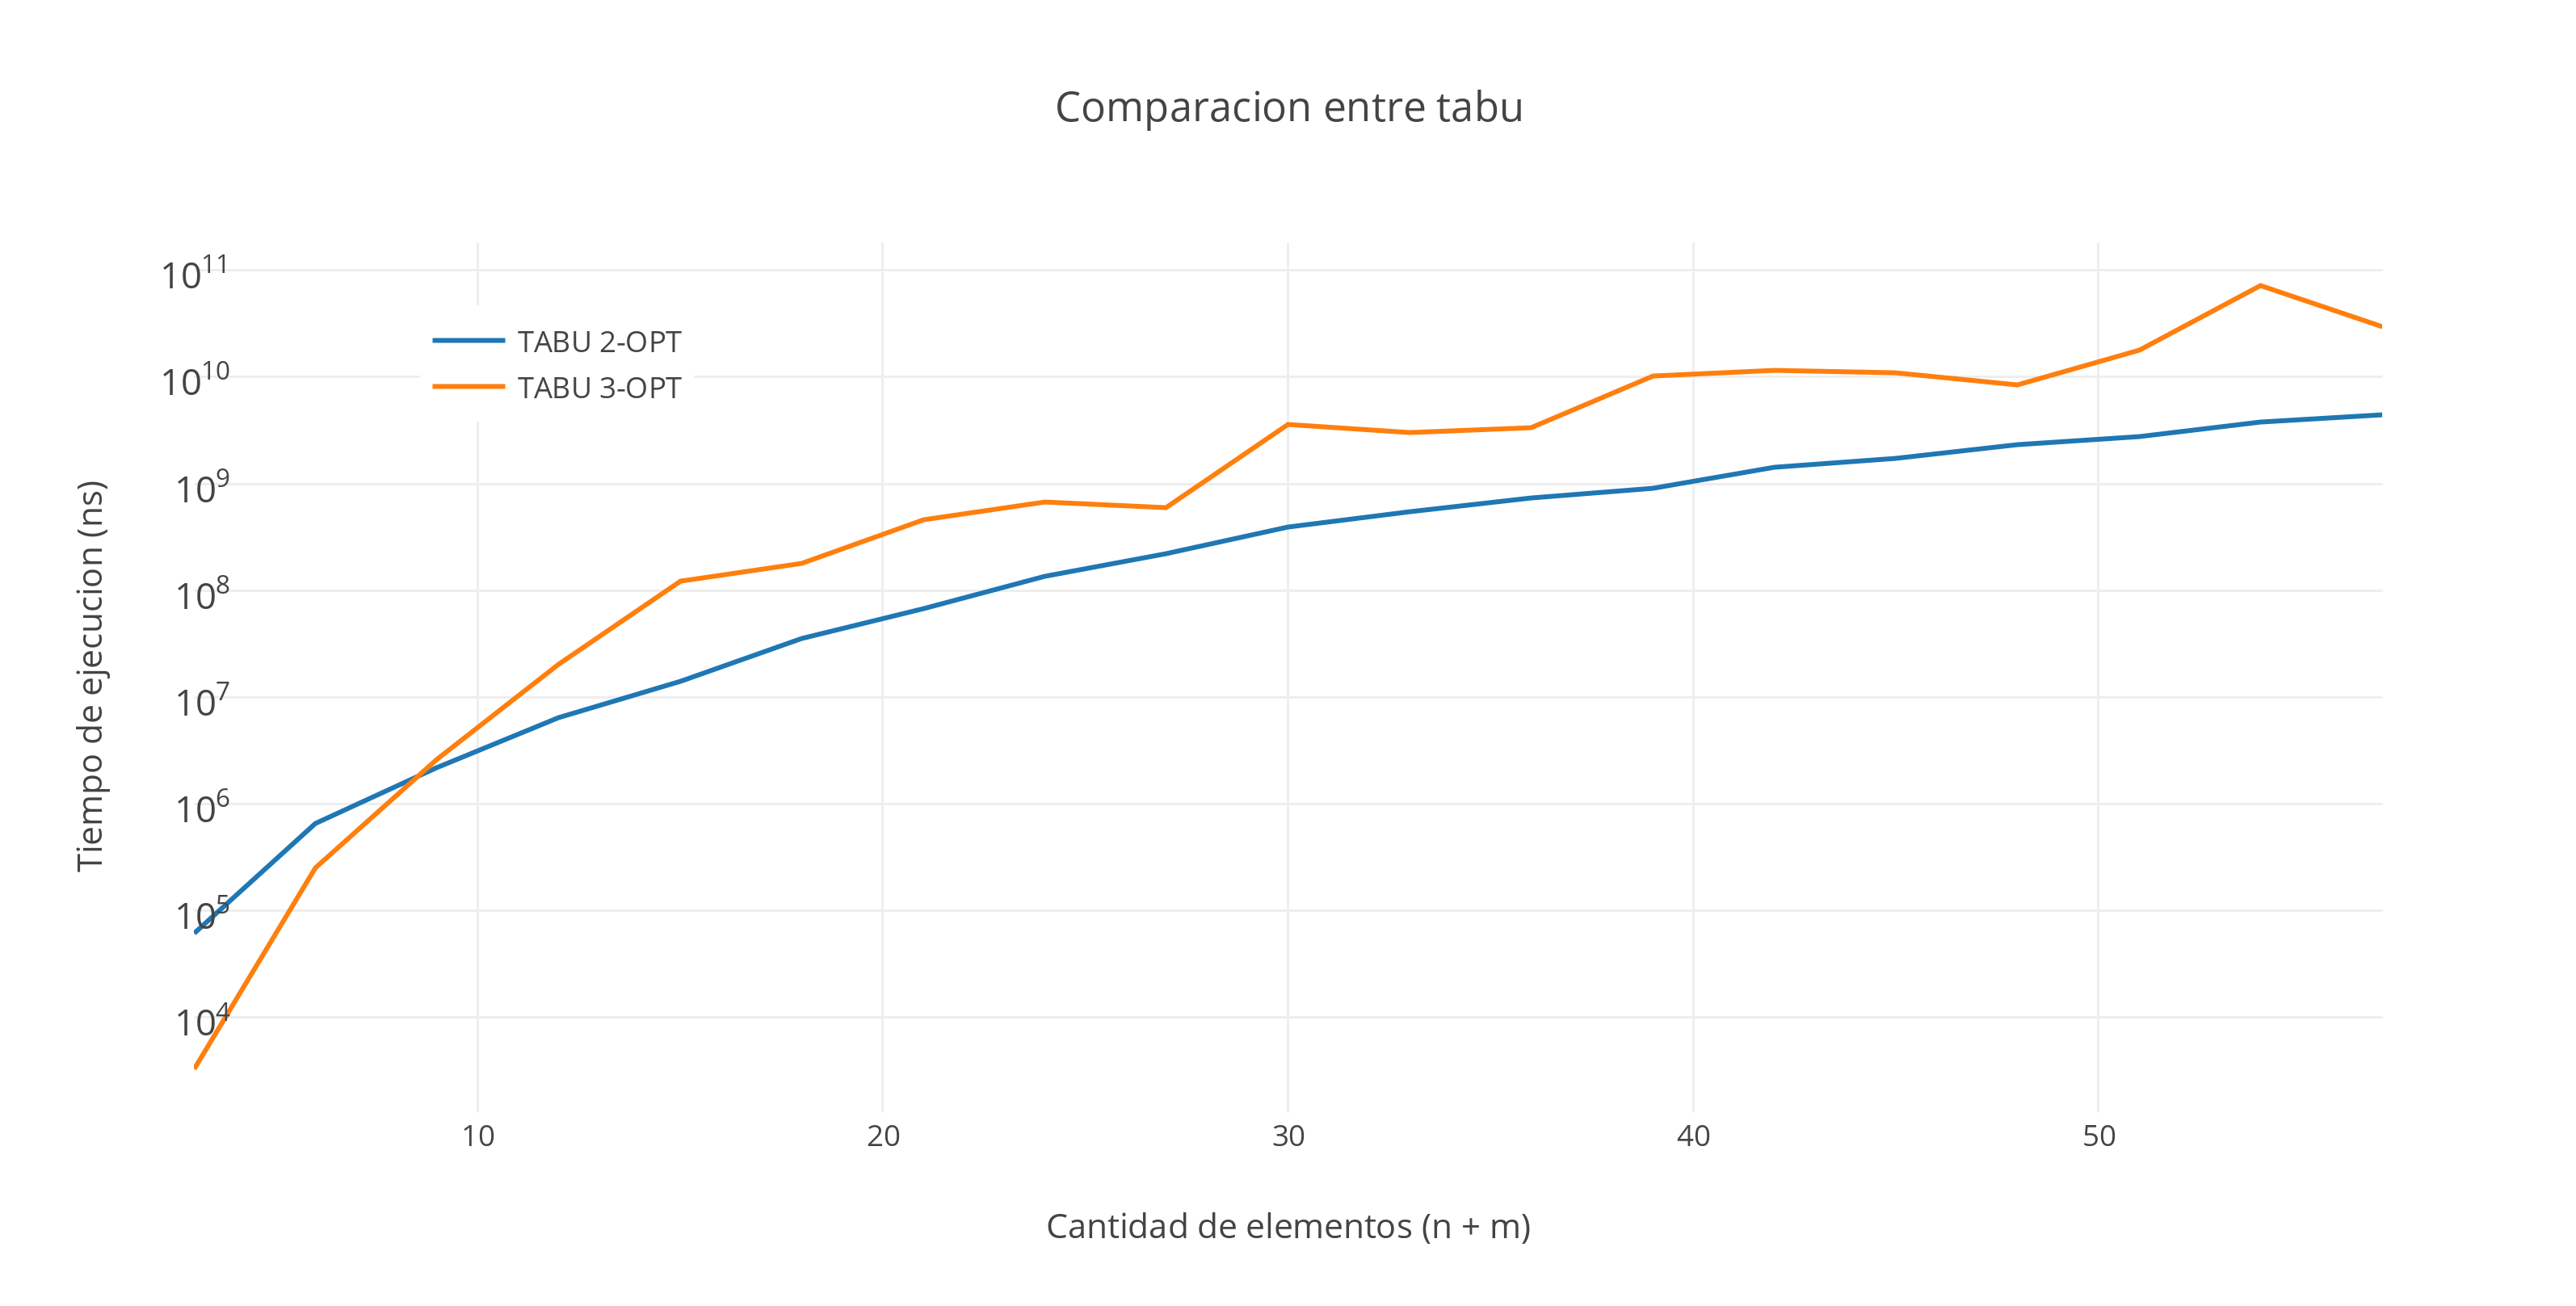
\includegraphics[scale=0.5]{./EJ4/comparacionsinorden1.png}\\
 {            \textit{Gráfico \ 4.12 - Tabu 2-OPT vs Tabu 3-OPT sobre Familia 6}}
  \end{center}
  \vspace*{0.3cm}
  
--> OBTENER CONCLUSIONES

\subsubsection*{Familia 7}

--> PRESENTAR FAMILIA

\vspace*{0.3cm} \vspace*{0.3cm}
  \begin{center}
 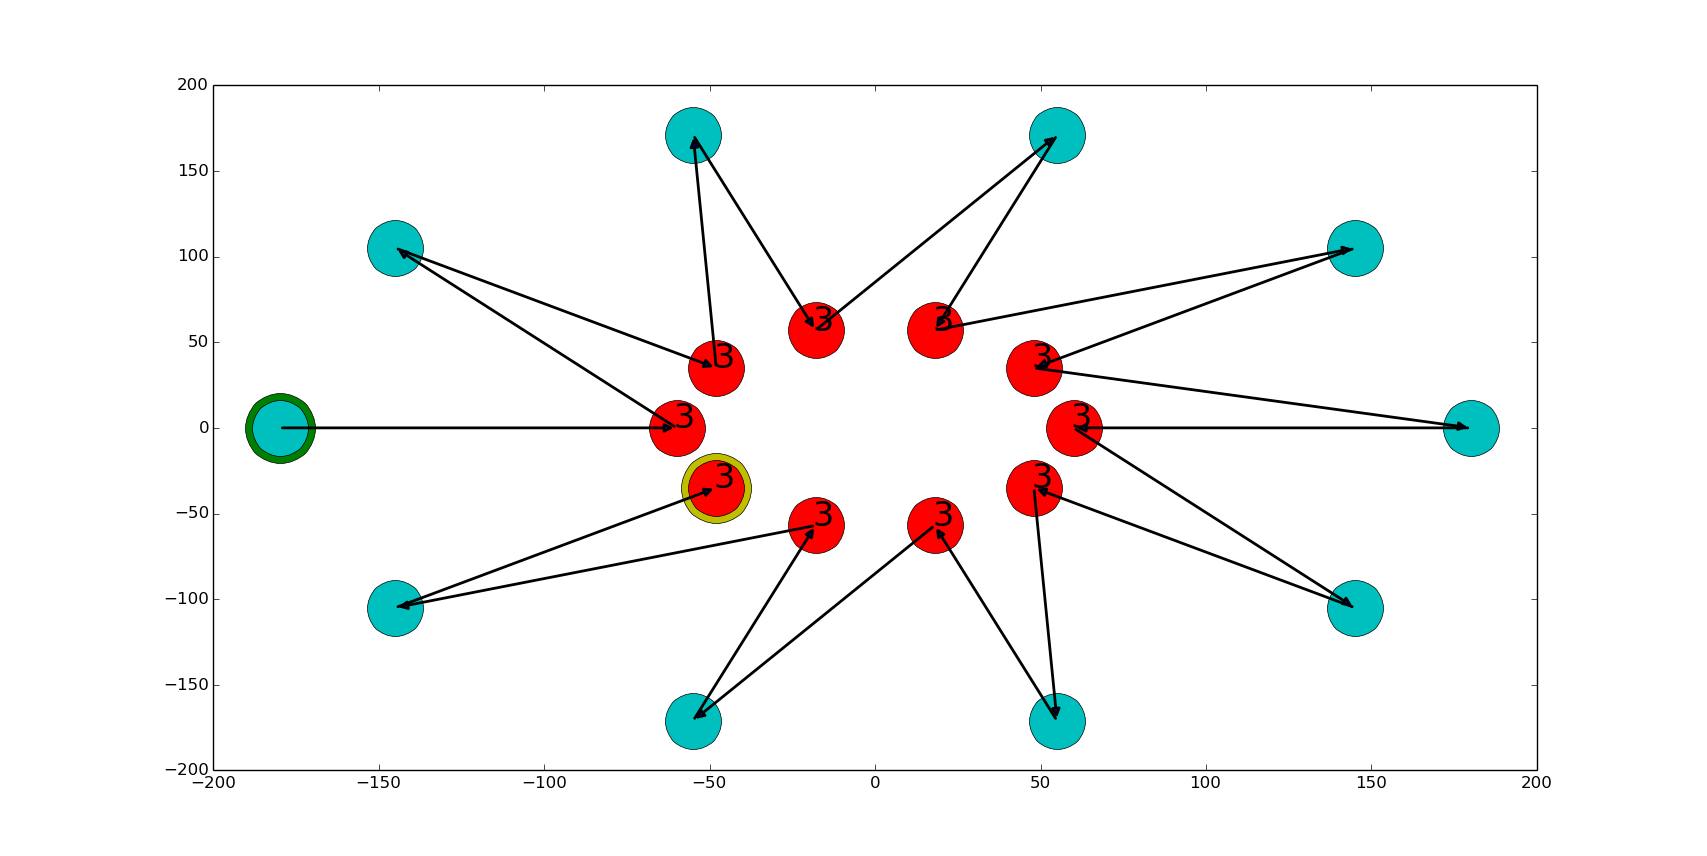
\includegraphics[scale=0.3]{./EJ4/fam7goloso.png}\\
 {            \textit{Soluci\'on Golosa}}
  \end{center}
  \vspace*{0.3cm}

\vspace*{0.3cm} \vspace*{0.3cm}
  \begin{center}
 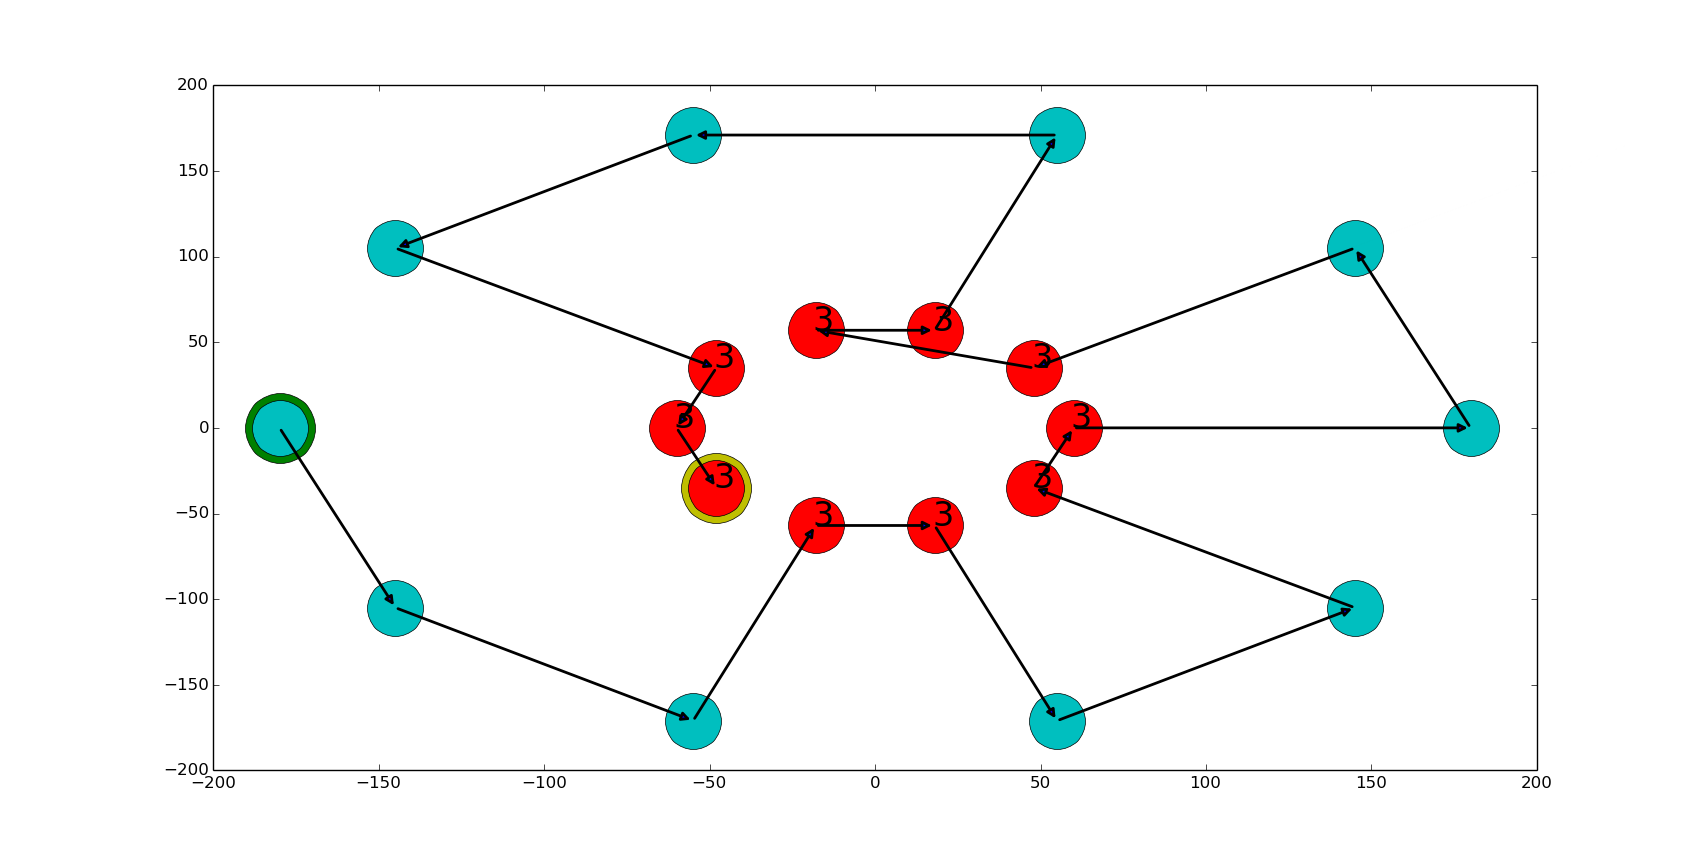
\includegraphics[scale=0.3]{./EJ4/fam72opt.png}\\
 {            \textit{Soluci\'on TABU 2-OPT}}
  \end{center}
  \vspace*{0.3cm}

\vspace*{0.3cm} \vspace*{0.3cm}
  \begin{center}
 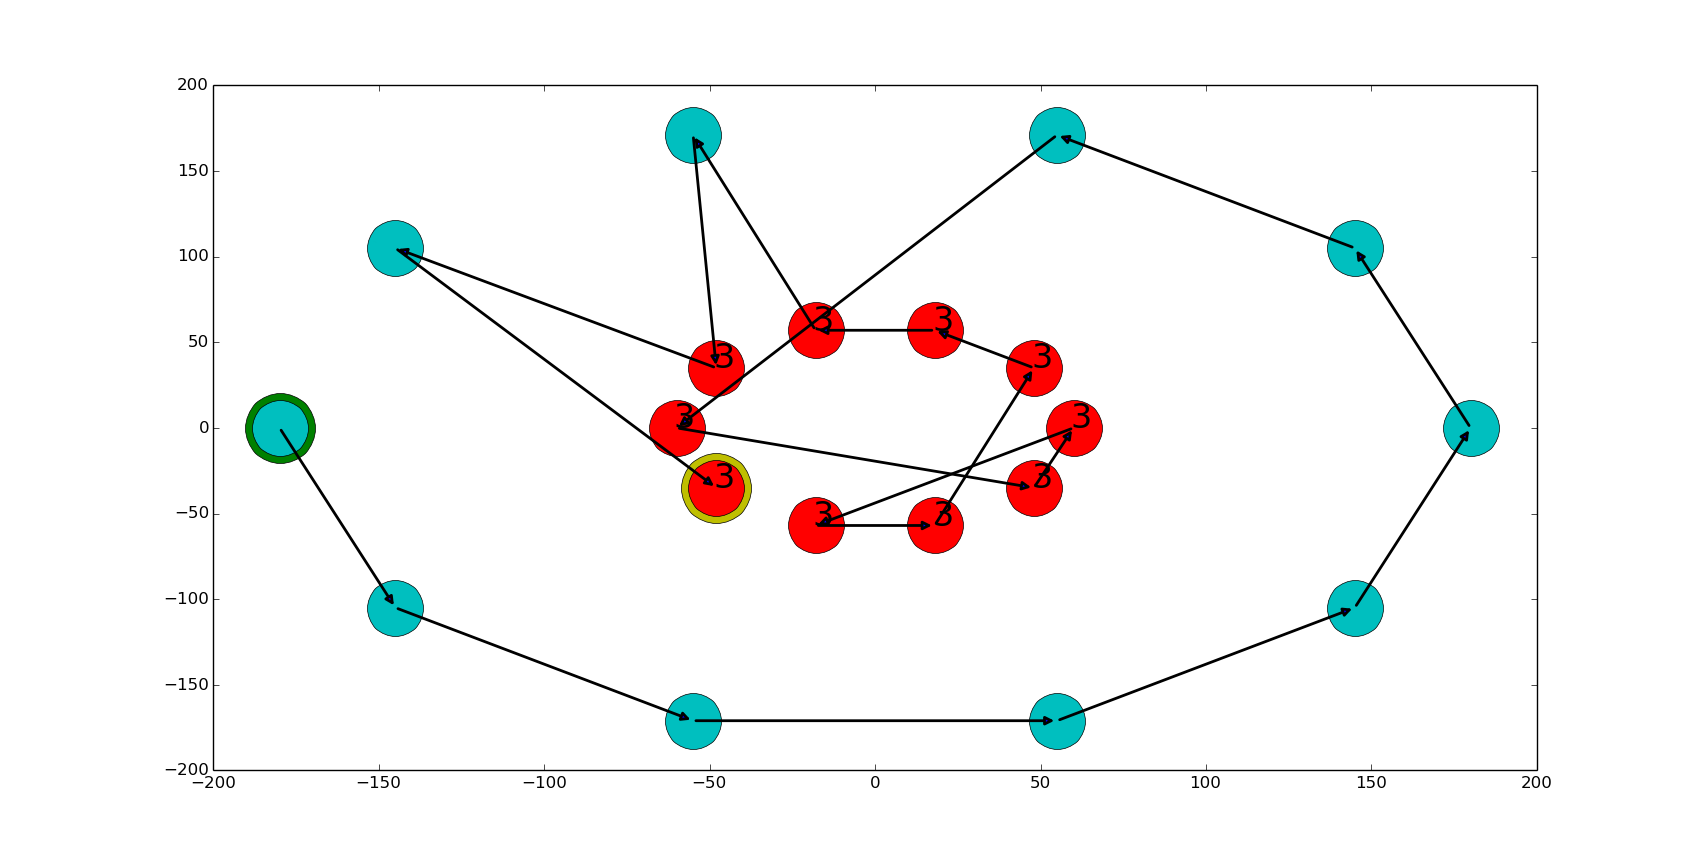
\includegraphics[scale=0.3]{./EJ4/fam73opt.png}\\
 {            \textit{Soluci\'on TABU 3-OPT}}
  \end{center}
  \vspace*{0.3cm}

Veamos como se comporta Tabu 2-OPT con respecto a la heuristica de busqueda local 2-OPT:

\vspace*{0.3cm} \vspace*{0.3cm}
  \begin{center}
 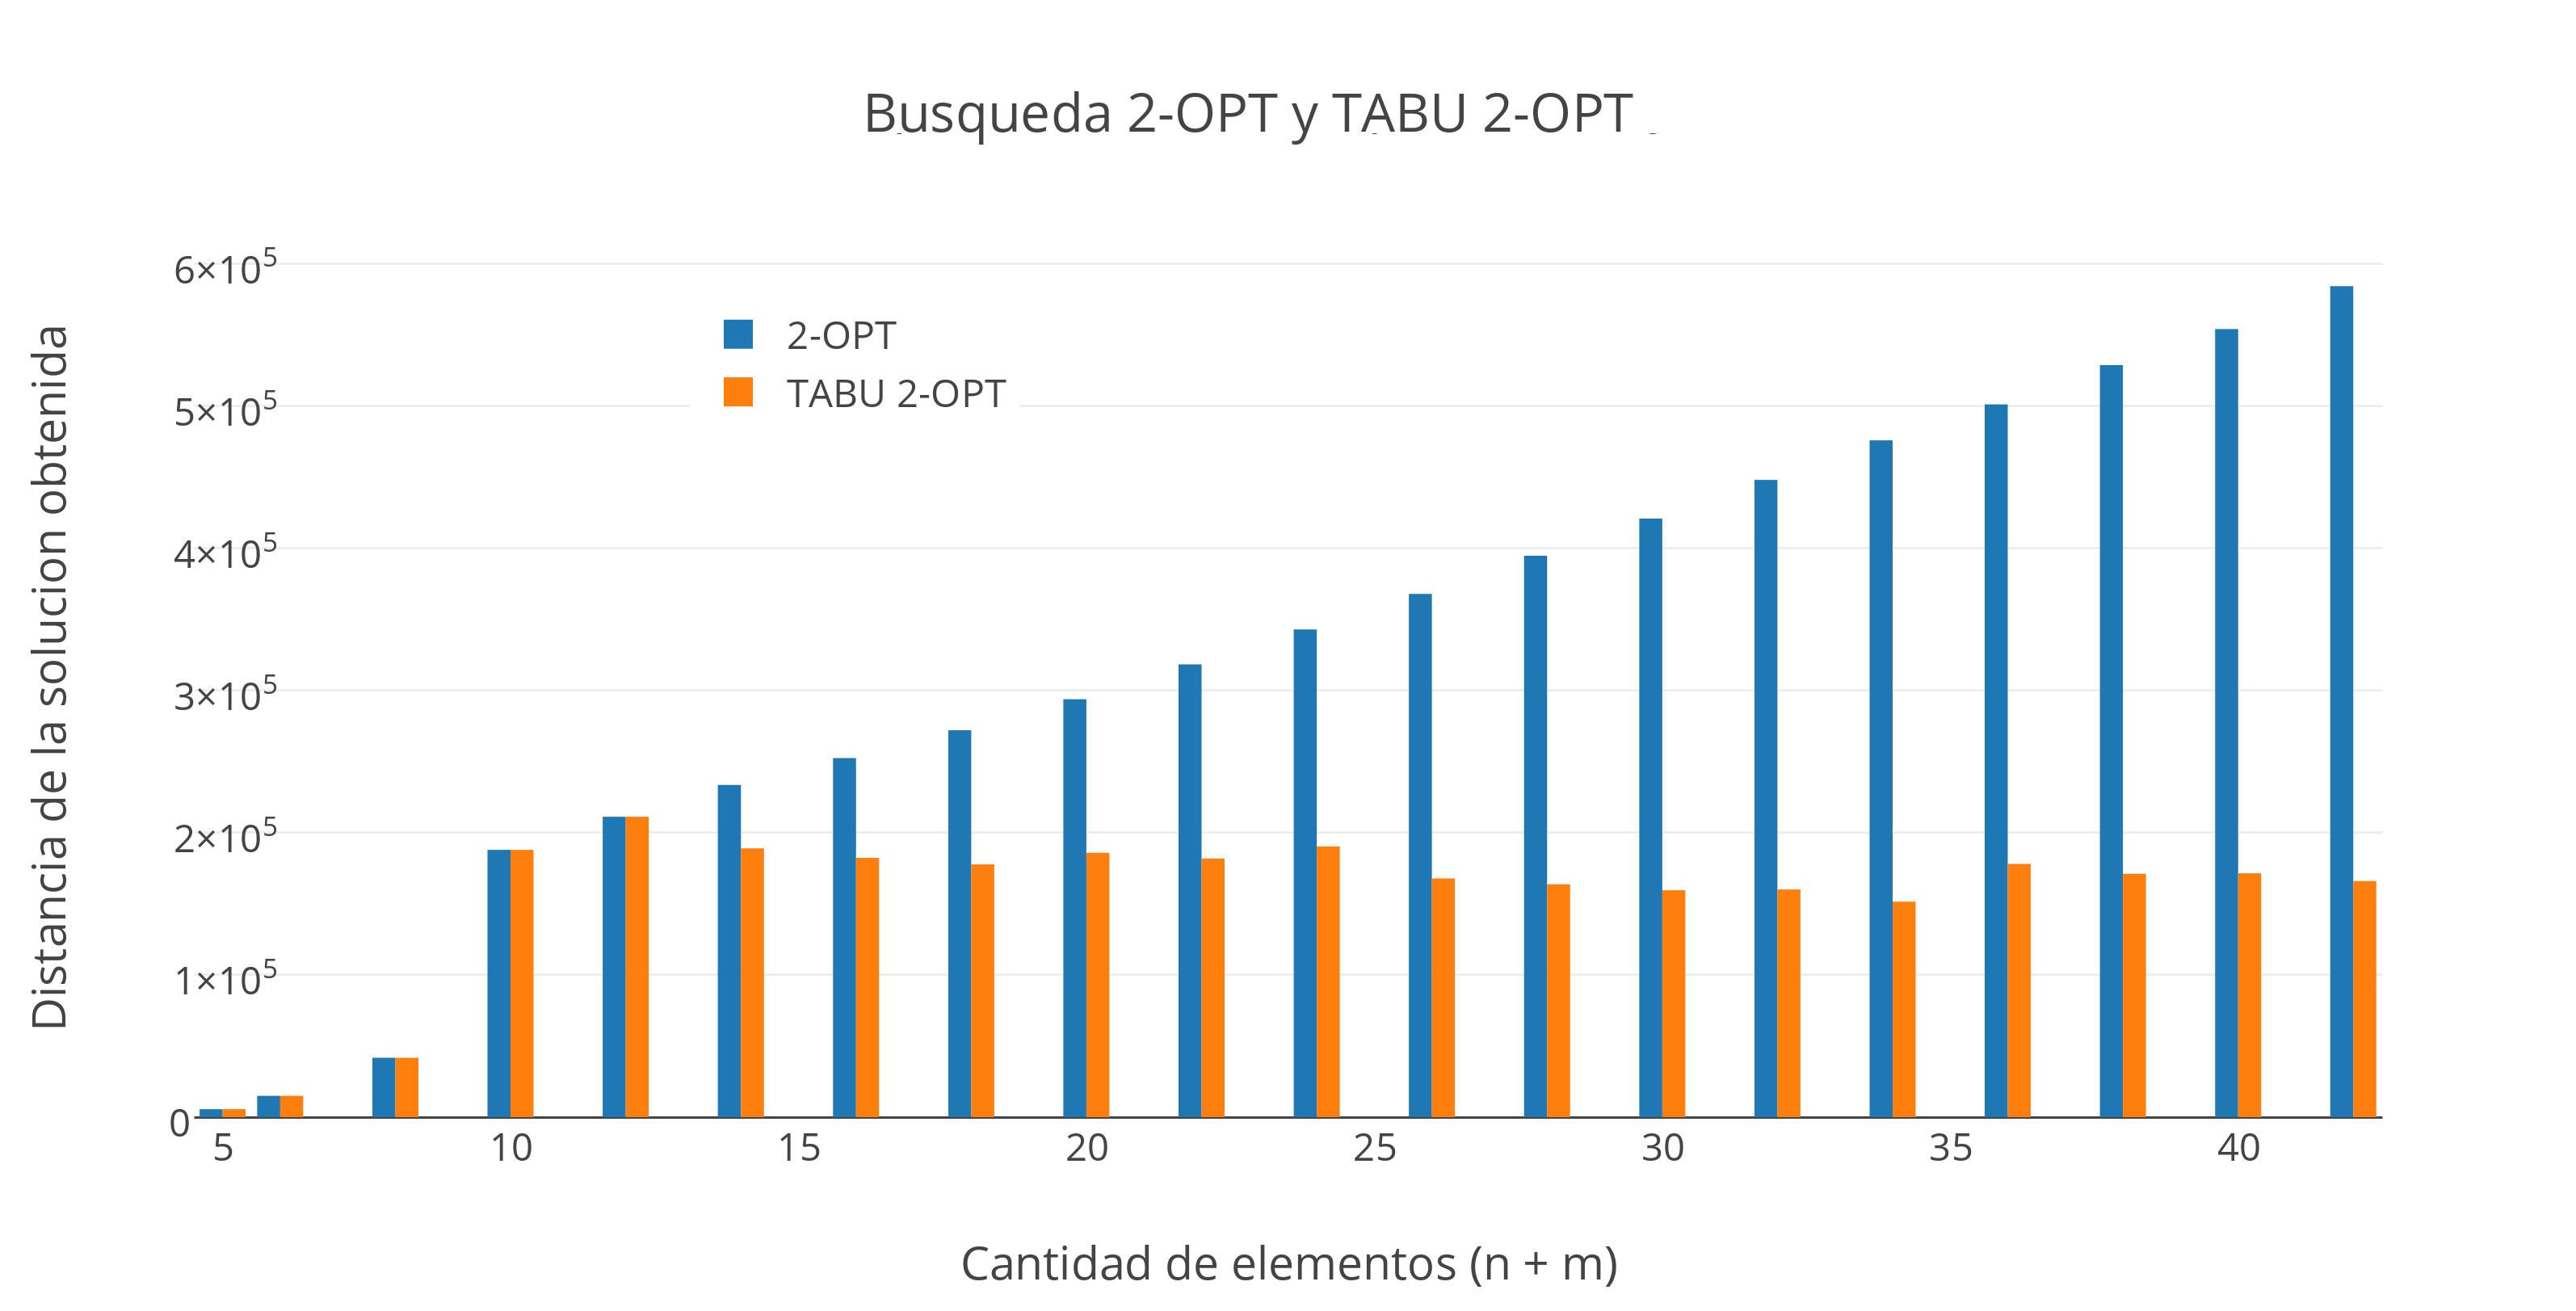
\includegraphics[scale=0.5]{./EJ4/comparativoanillos2opt.png}\\
 {            \textit{Gráfico \ 4.7 - 2-OPT vs Tabu 2-OPT sobre Familia 7}}
  \end{center}
  \vspace*{0.3cm}

\vspace*{0.3cm} \vspace*{0.3cm}
  \begin{center}
 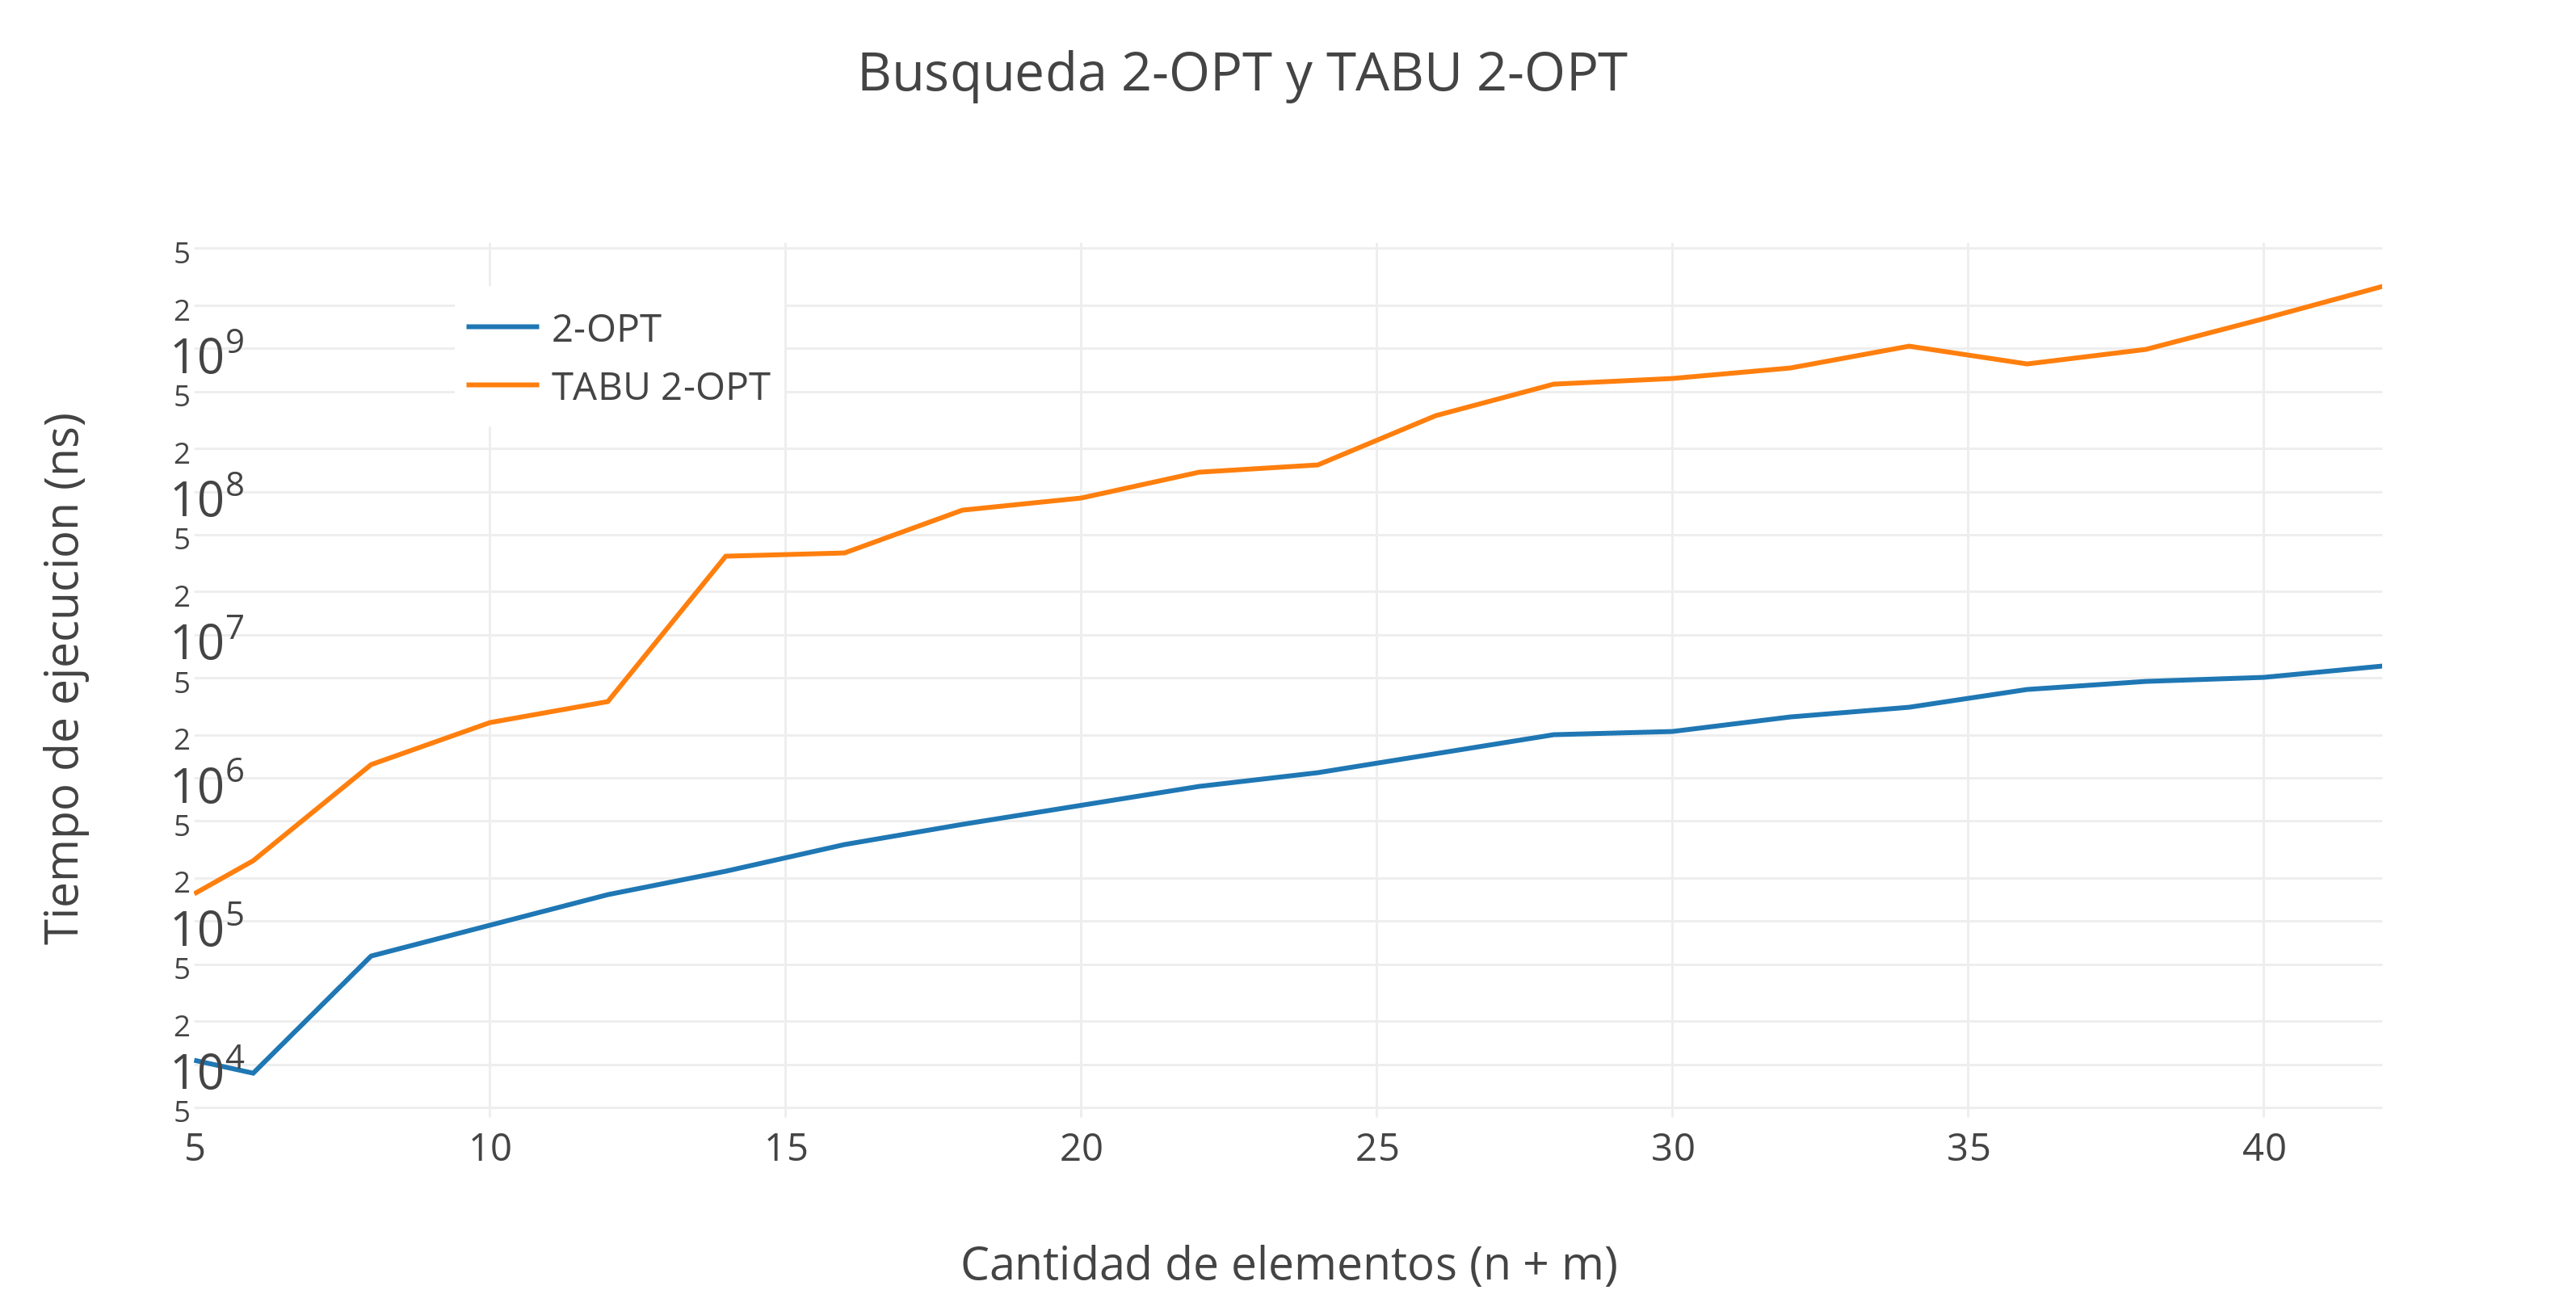
\includegraphics[scale=0.5]{./EJ4/medicionanillos2opt.png}\\
 {            \textit{Gráfico \ 4.8 - 2-OPT vs Tabu 2-OPT sobre Familia 7}}
  \end{center}
  \vspace*{0.3cm}

Luego, para 3-OPT:

\vspace*{0.3cm} \vspace*{0.3cm}
  \begin{center}
 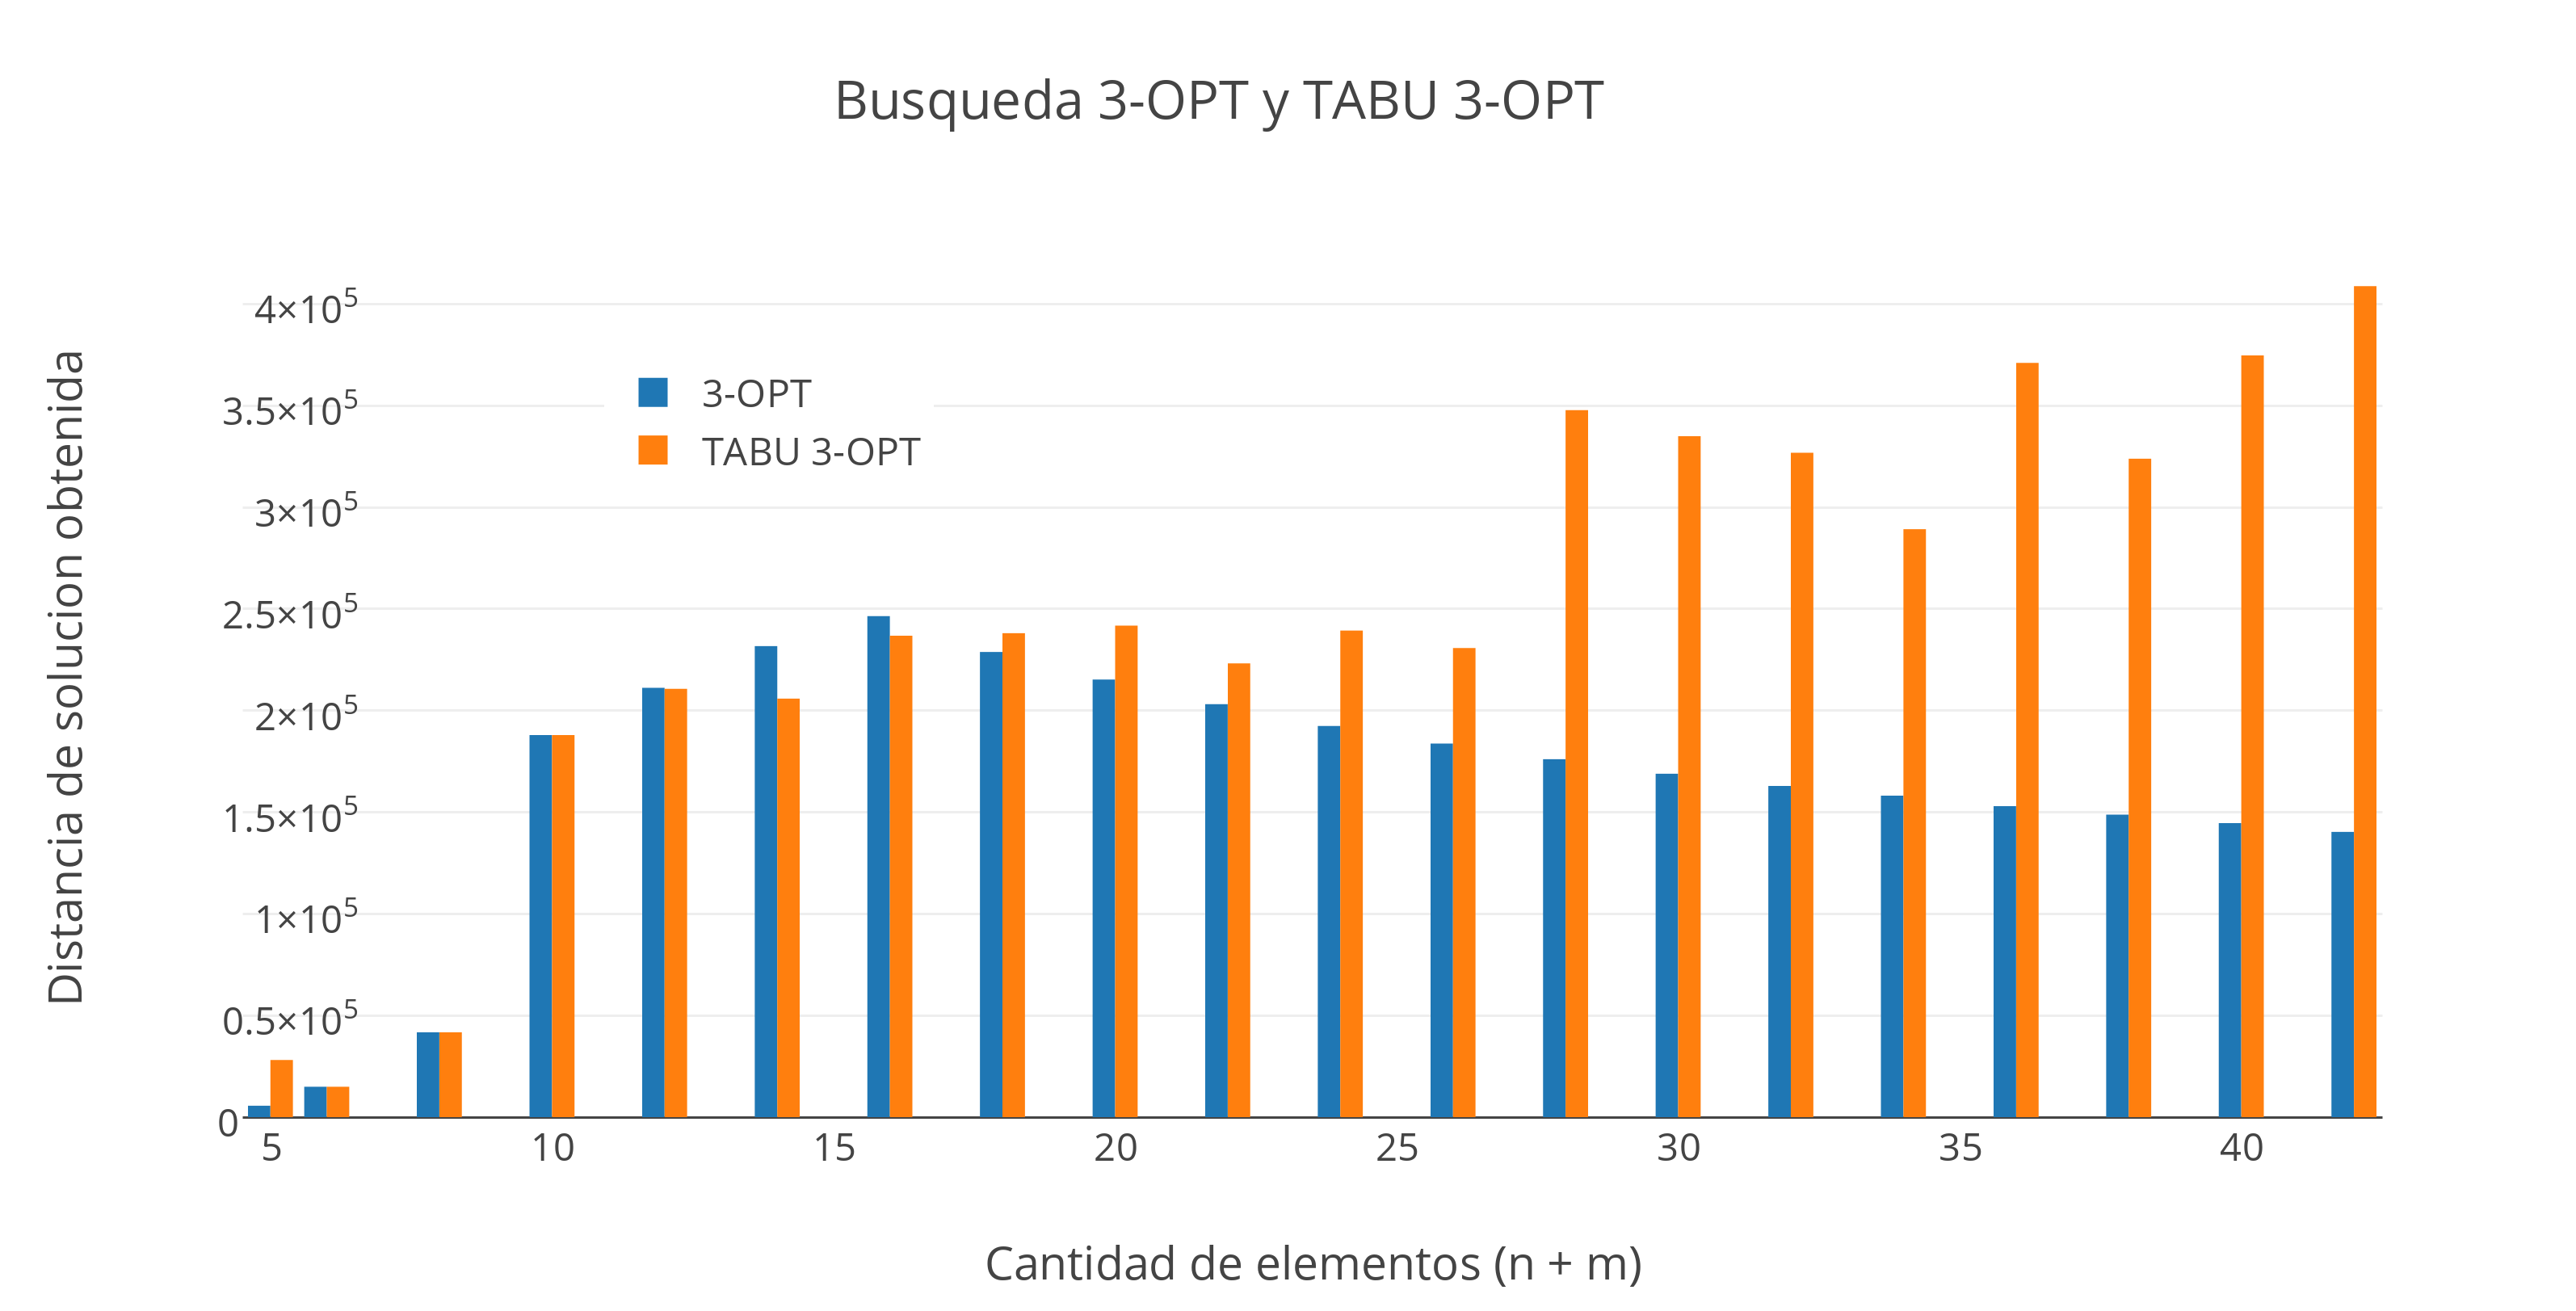
\includegraphics[scale=0.5]{./EJ4/comparativoanillos3opt.png}\\
 {            \textit{Gráfico \ 4.9 - 3-OPT vs Tabu 3-OPT sobre Familia 7}}
  \end{center}
  \vspace*{0.3cm}

\vspace*{0.3cm} \vspace*{0.3cm}
  \begin{center}
 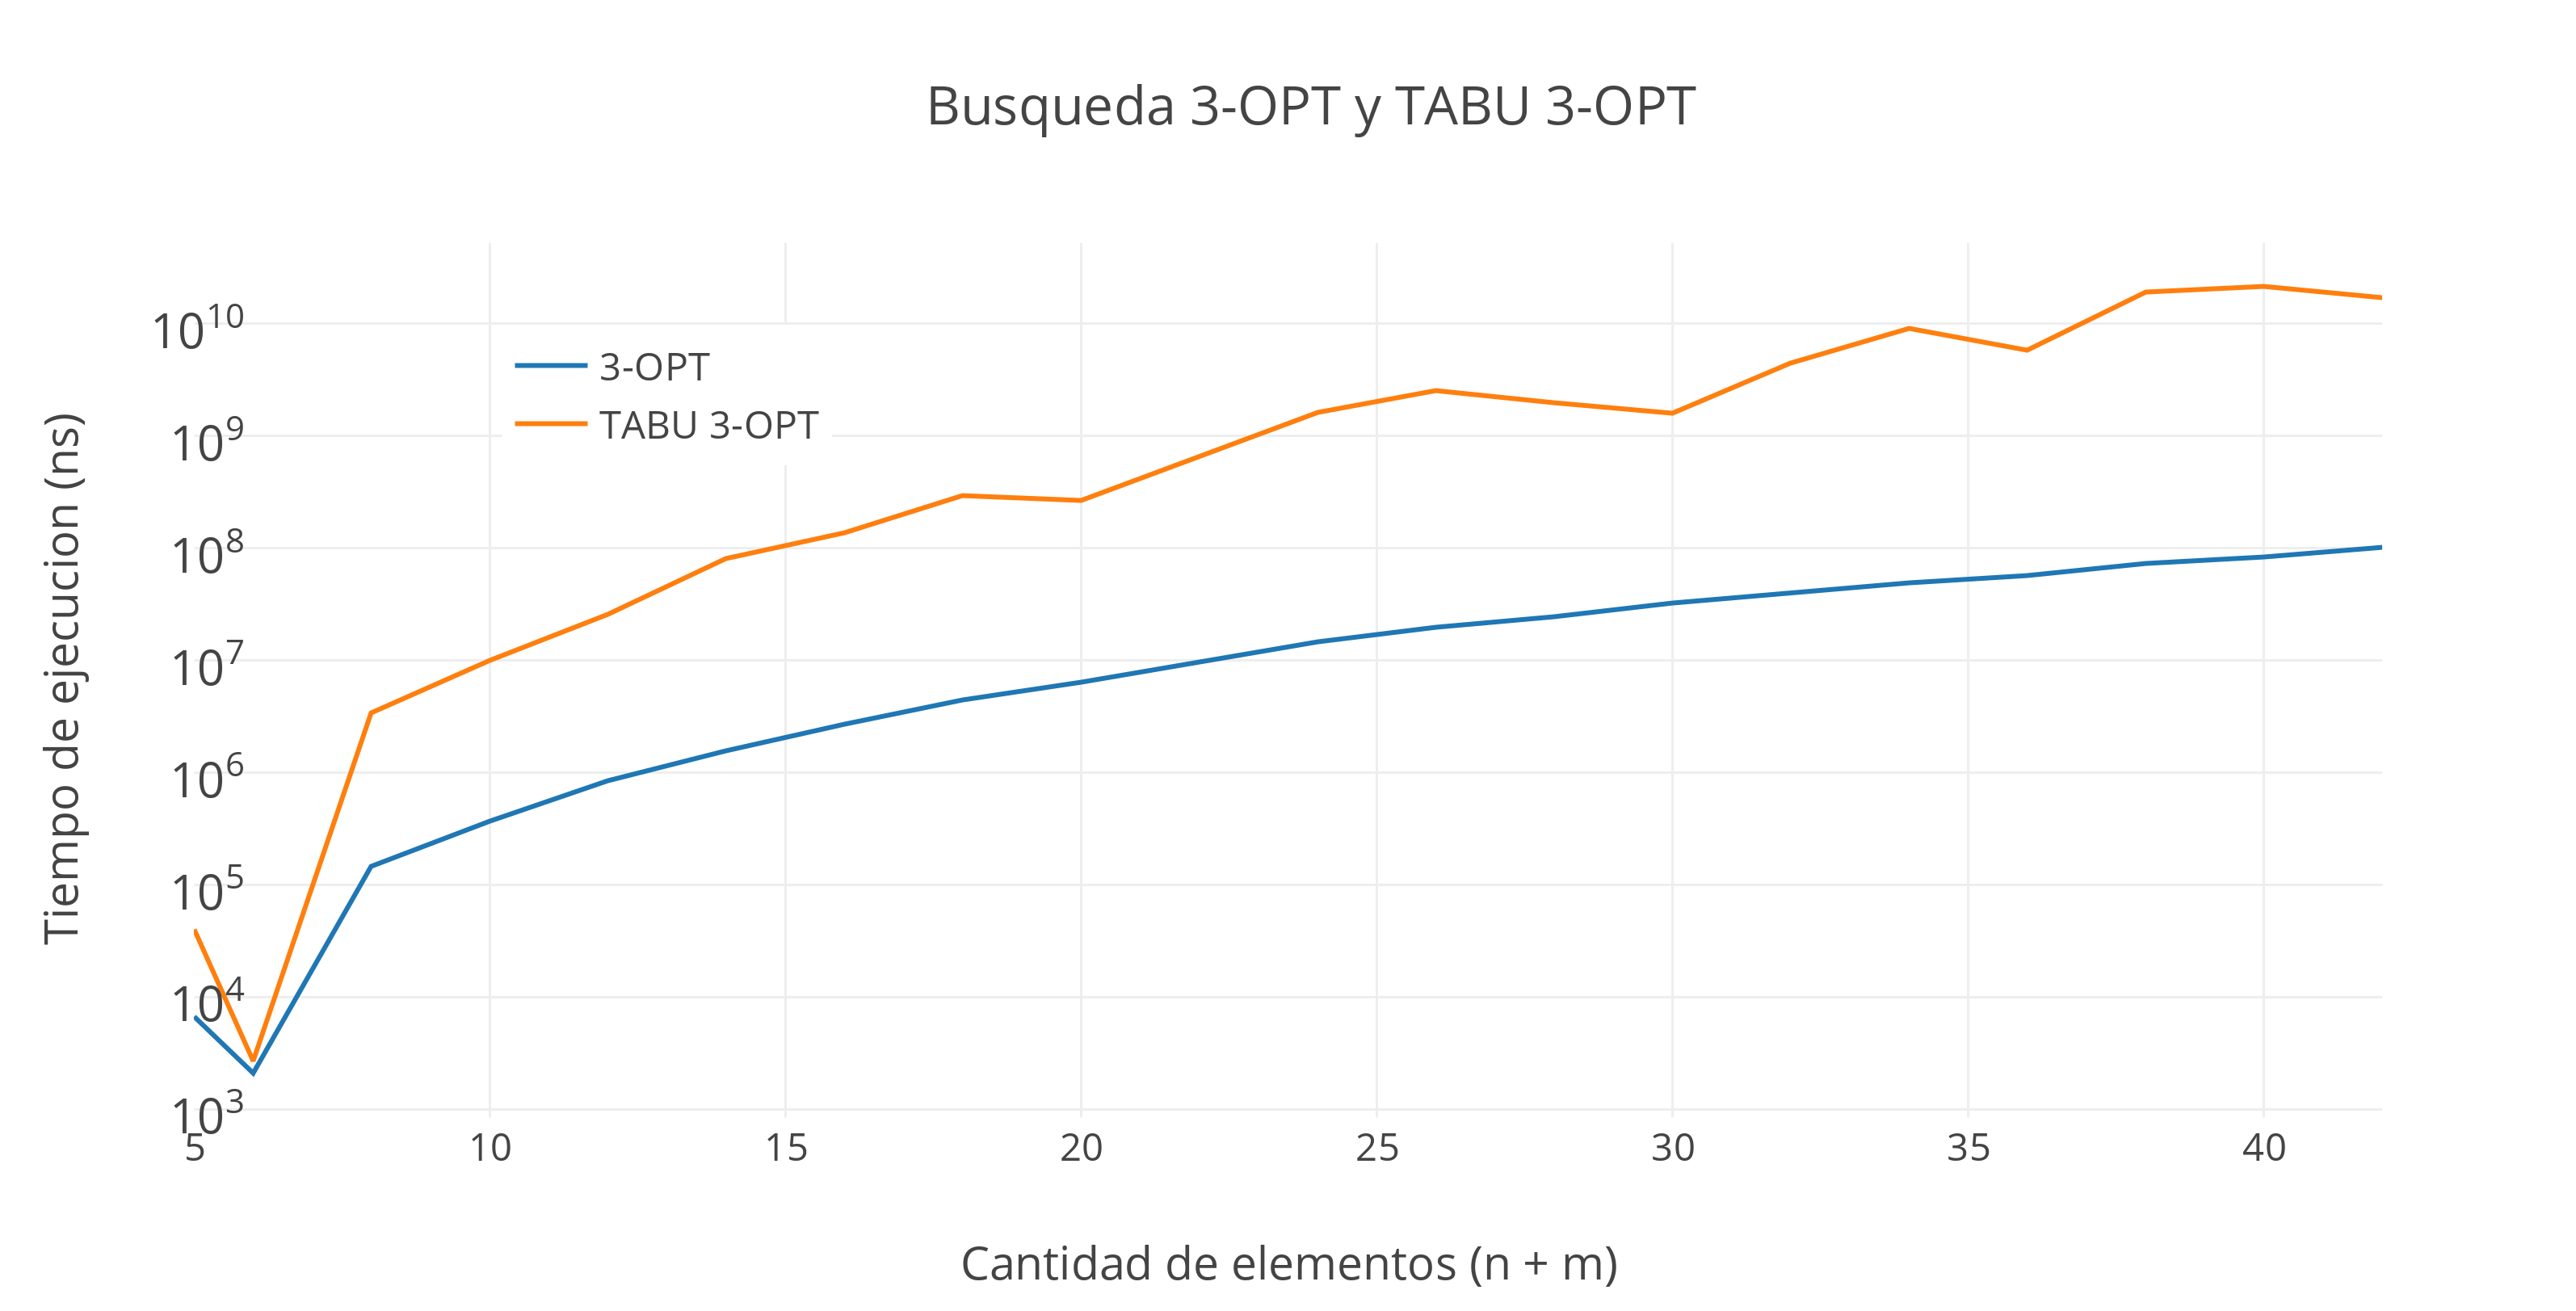
\includegraphics[scale=0.5]{./EJ4/medicionanillos3opt.png}\\
 {            \textit{Gráfico \ 4.10 - 3-OPT vs Tabu 3-OPT sobre Familia 7}}
  \end{center}
  \vspace*{0.3cm}
  
--> OBTENER CONCLUSIONES  
 
Comparando las soluciones de cada version de tabú search podemos observar lo siguiente: 
  
\vspace*{0.3cm} \vspace*{0.3cm}
  \begin{center}
 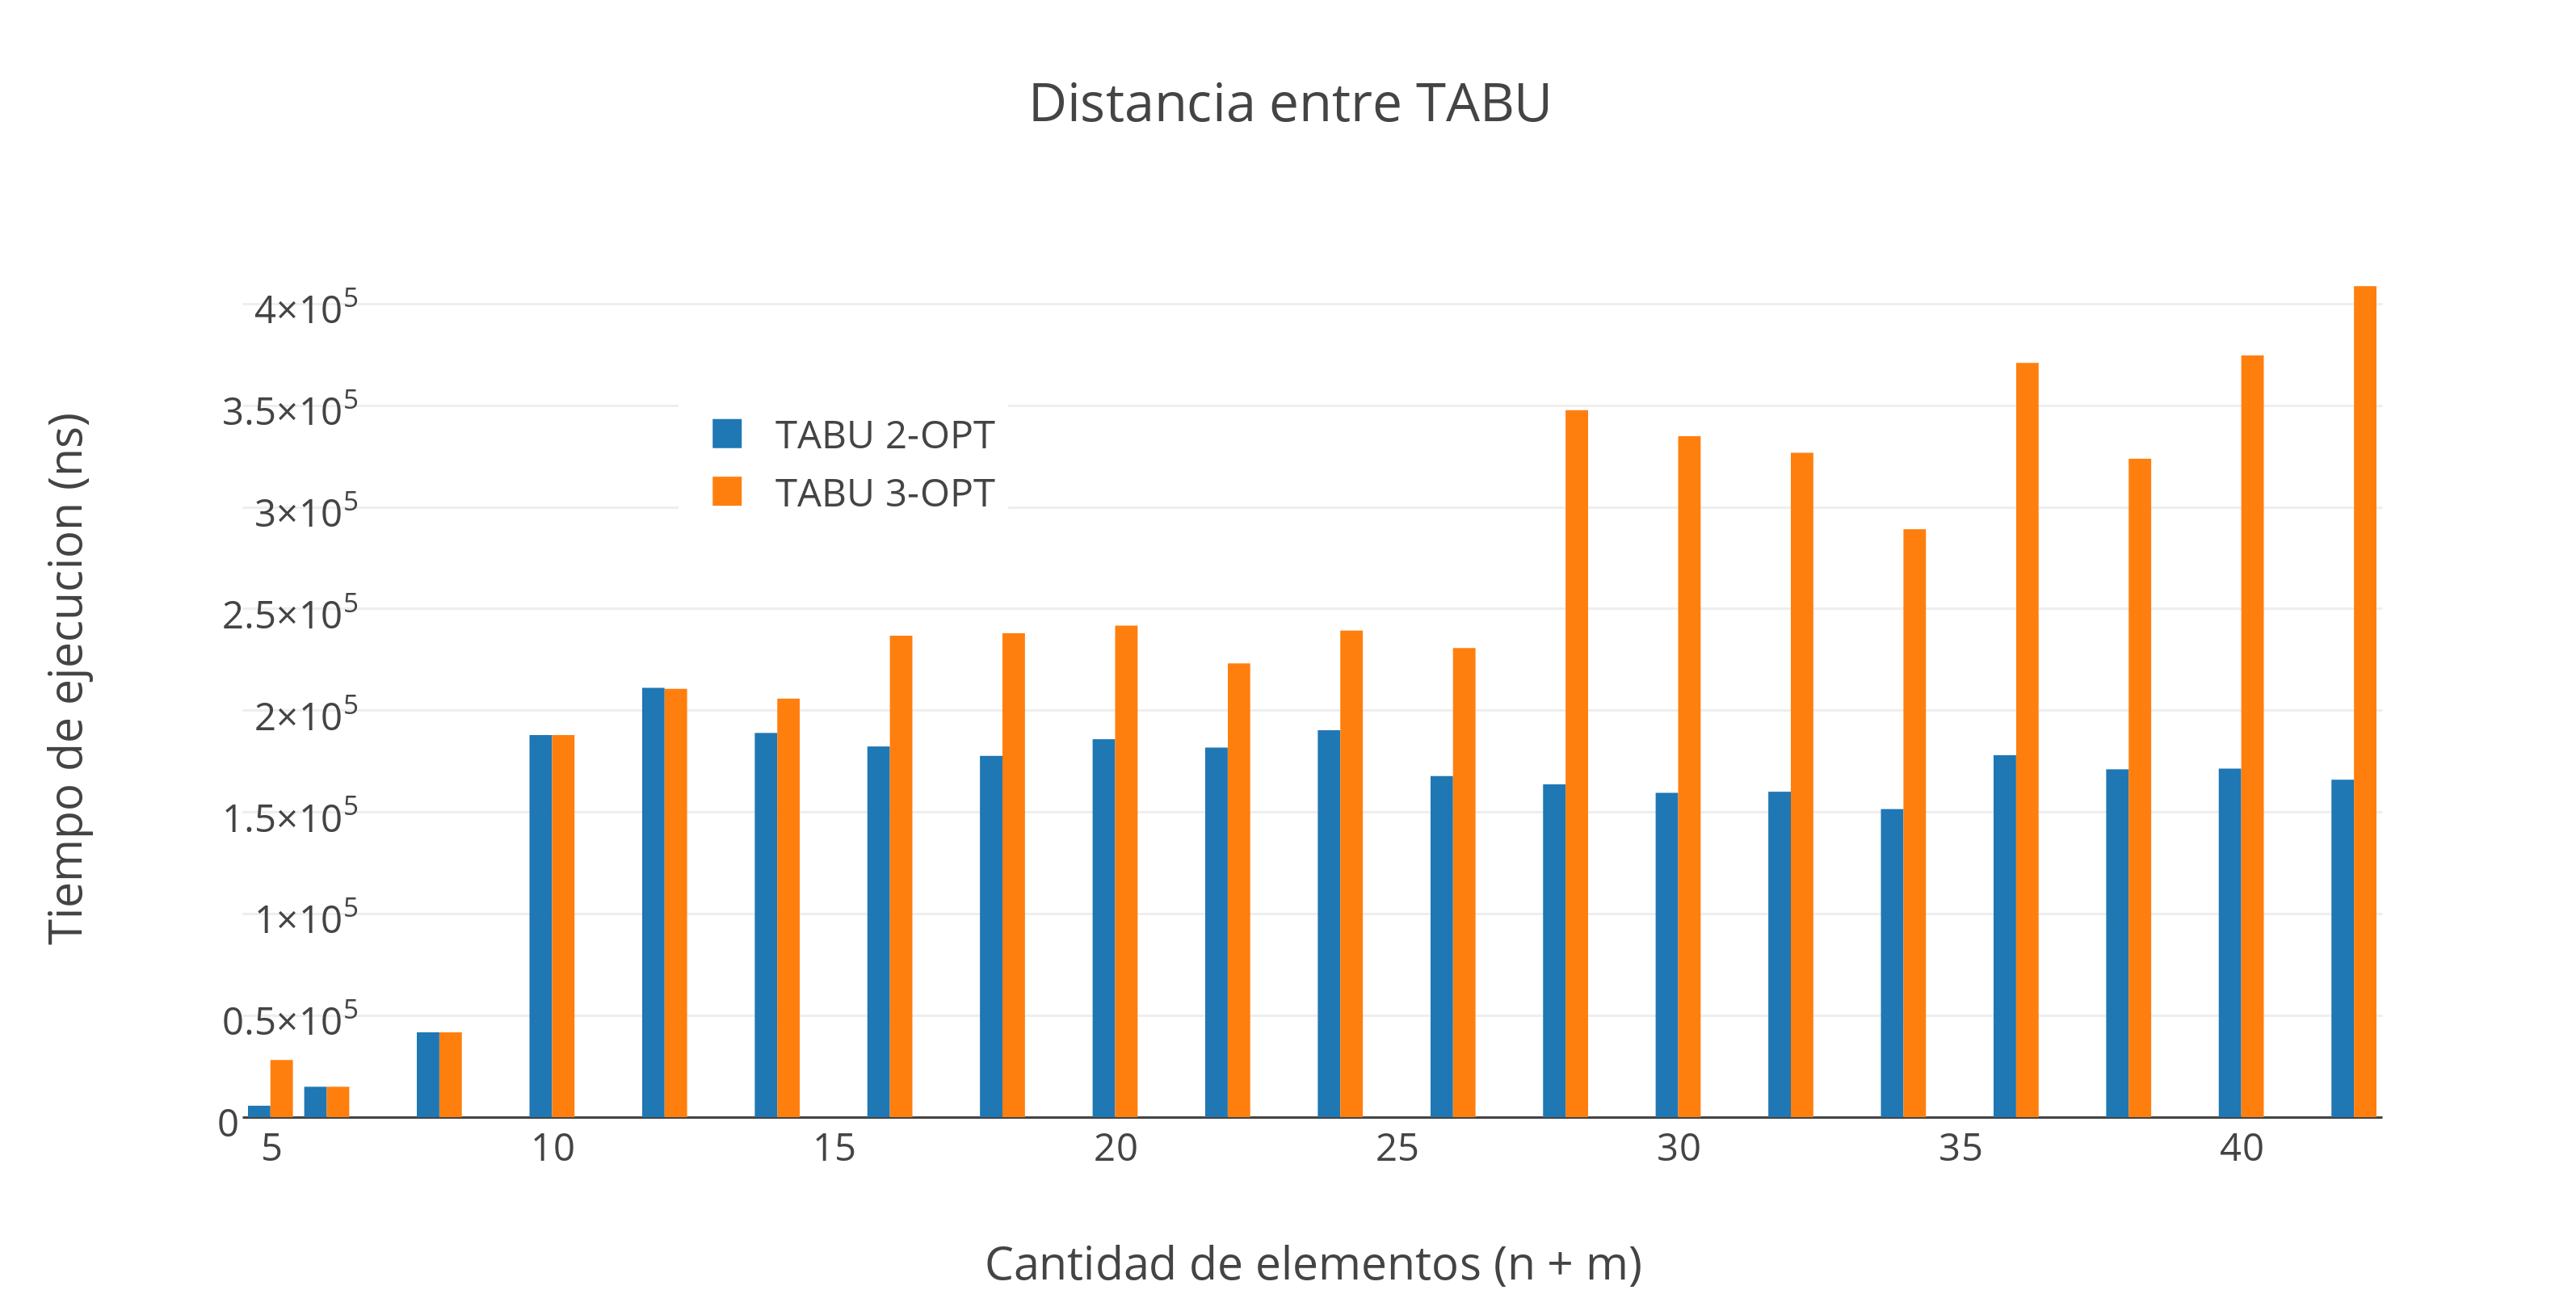
\includegraphics[scale=0.5]{./EJ4/comparativoanillos1.png}\\
 {            \textit{Gráfico \ 4.11 - Tabu 2-OPT vs Tabu 3-OPT sobre Familia 7}}
  \end{center}
  \vspace*{0.3cm}

\vspace*{0.3cm} \vspace*{0.3cm}
  \begin{center}
 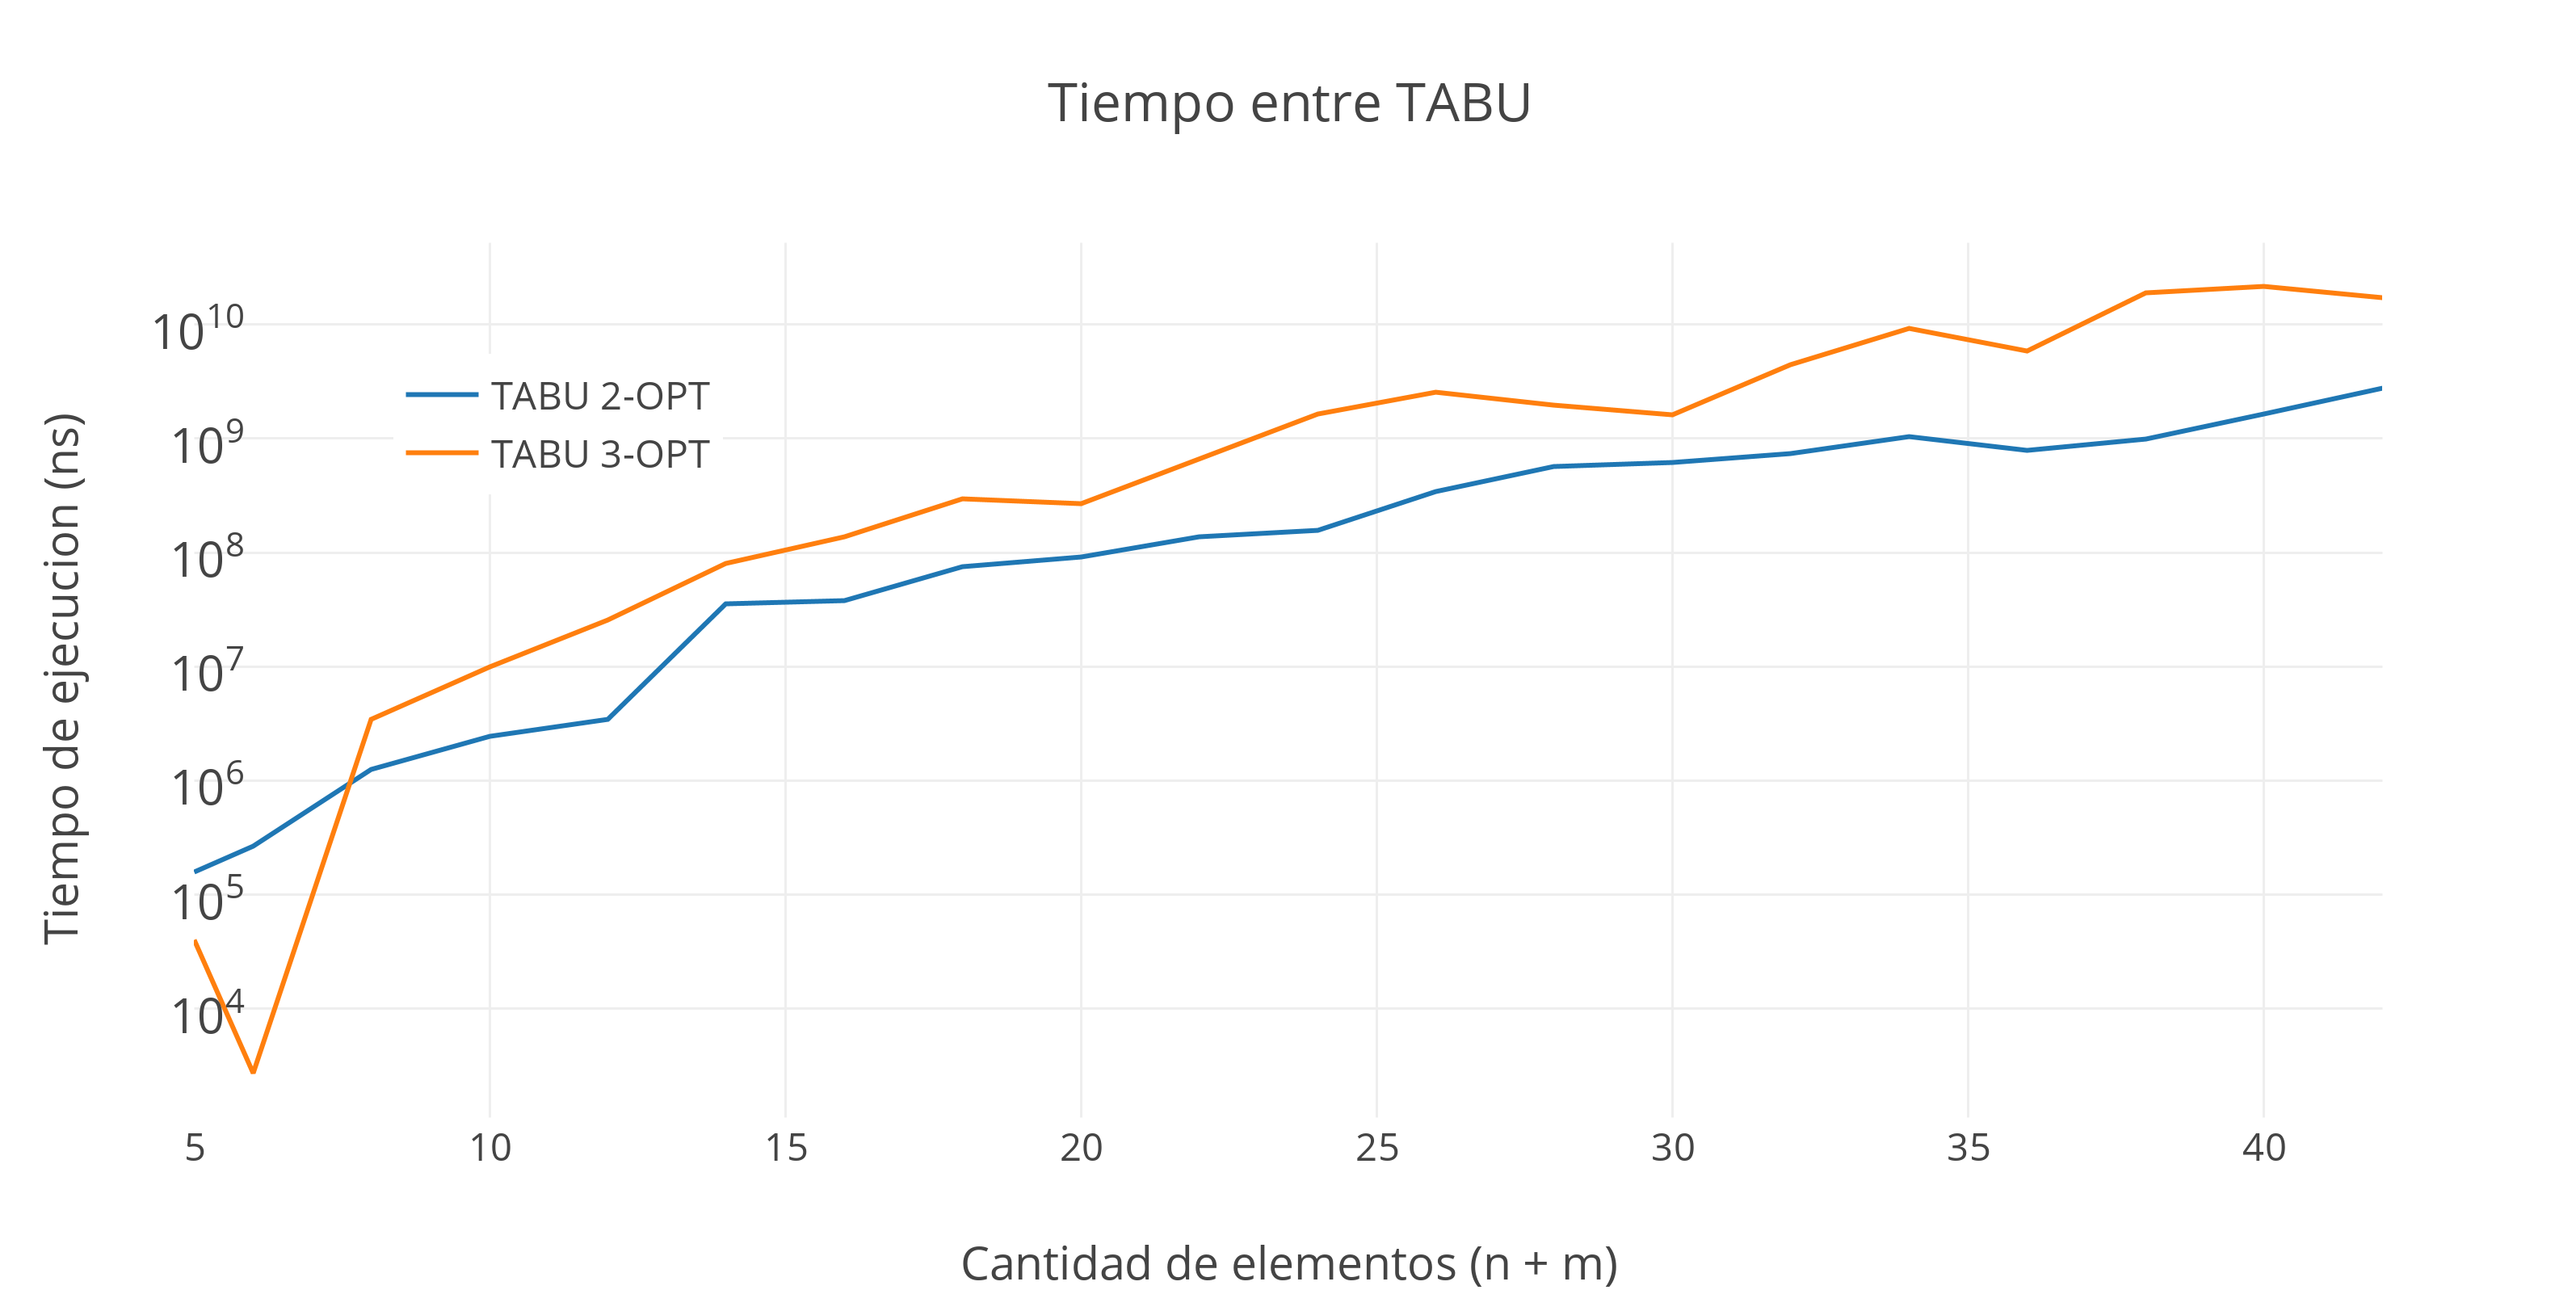
\includegraphics[scale=0.5]{./EJ4/comparativoanillos.png}\\
 {            \textit{Gráfico \ 4.12 - Tabu 2-OPT vs Tabu 3-OPT sobre Familia 7}}
  \end{center}
  \vspace*{0.3cm}

\subsubsection*{Familia 8}

--> PRESENTAR FAMILIA

\vspace*{0.3cm} \vspace*{0.3cm}
  \begin{center}
 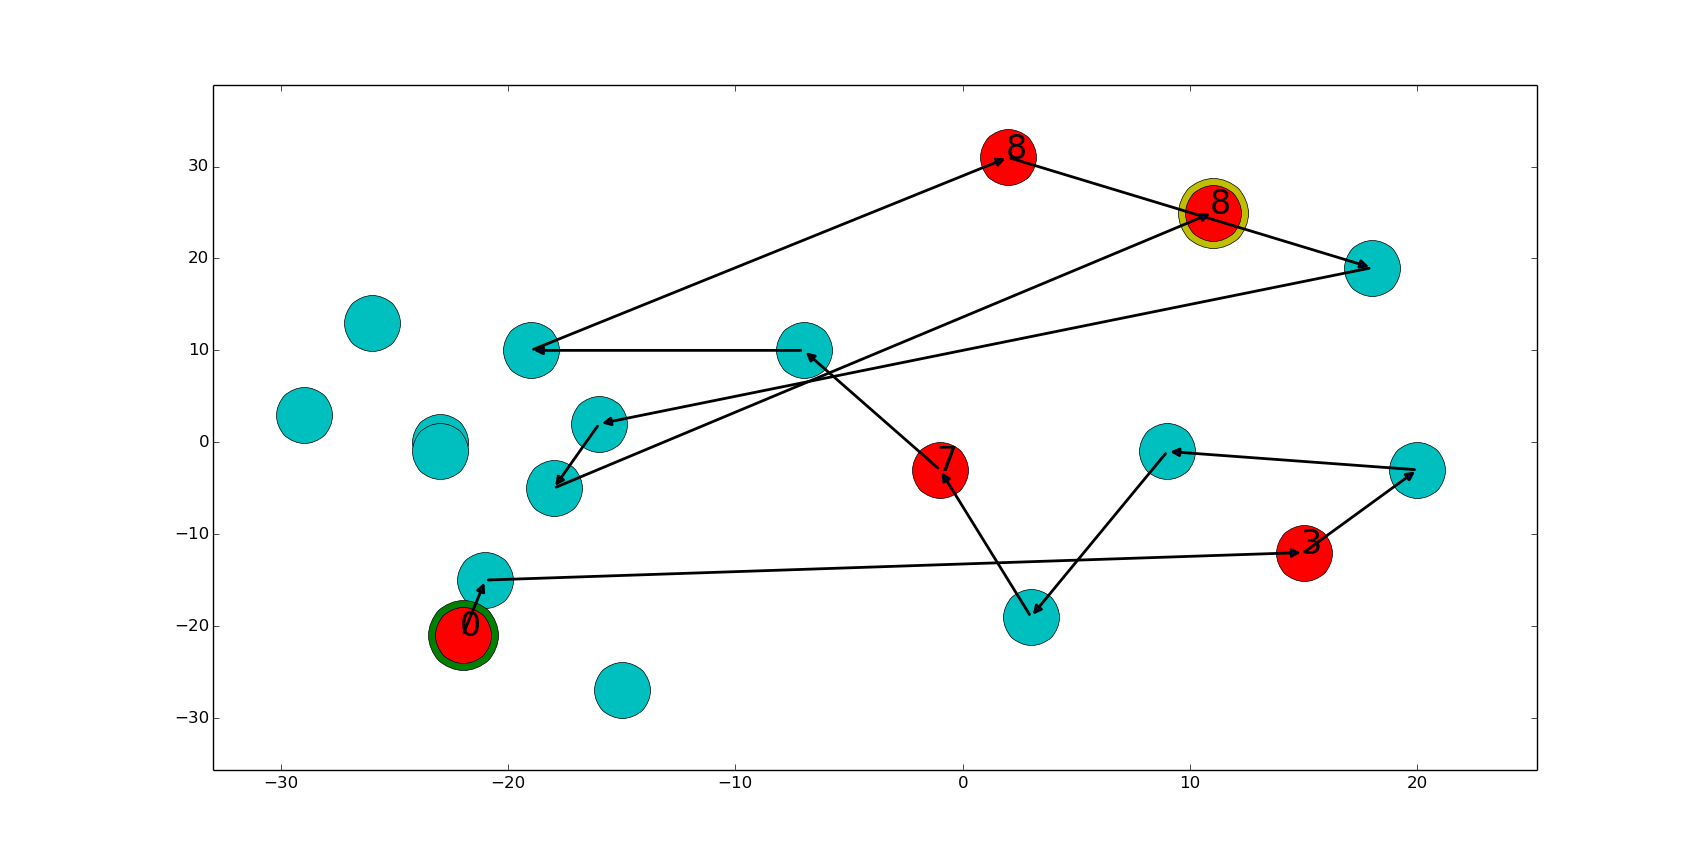
\includegraphics[scale=0.3]{./EJ4/fam8goloso.png}\\
 {            \textit{Soluci\'on Golosa}}
  \end{center}
  \vspace*{0.3cm}

\vspace*{0.3cm} \vspace*{0.3cm}
  \begin{center}
 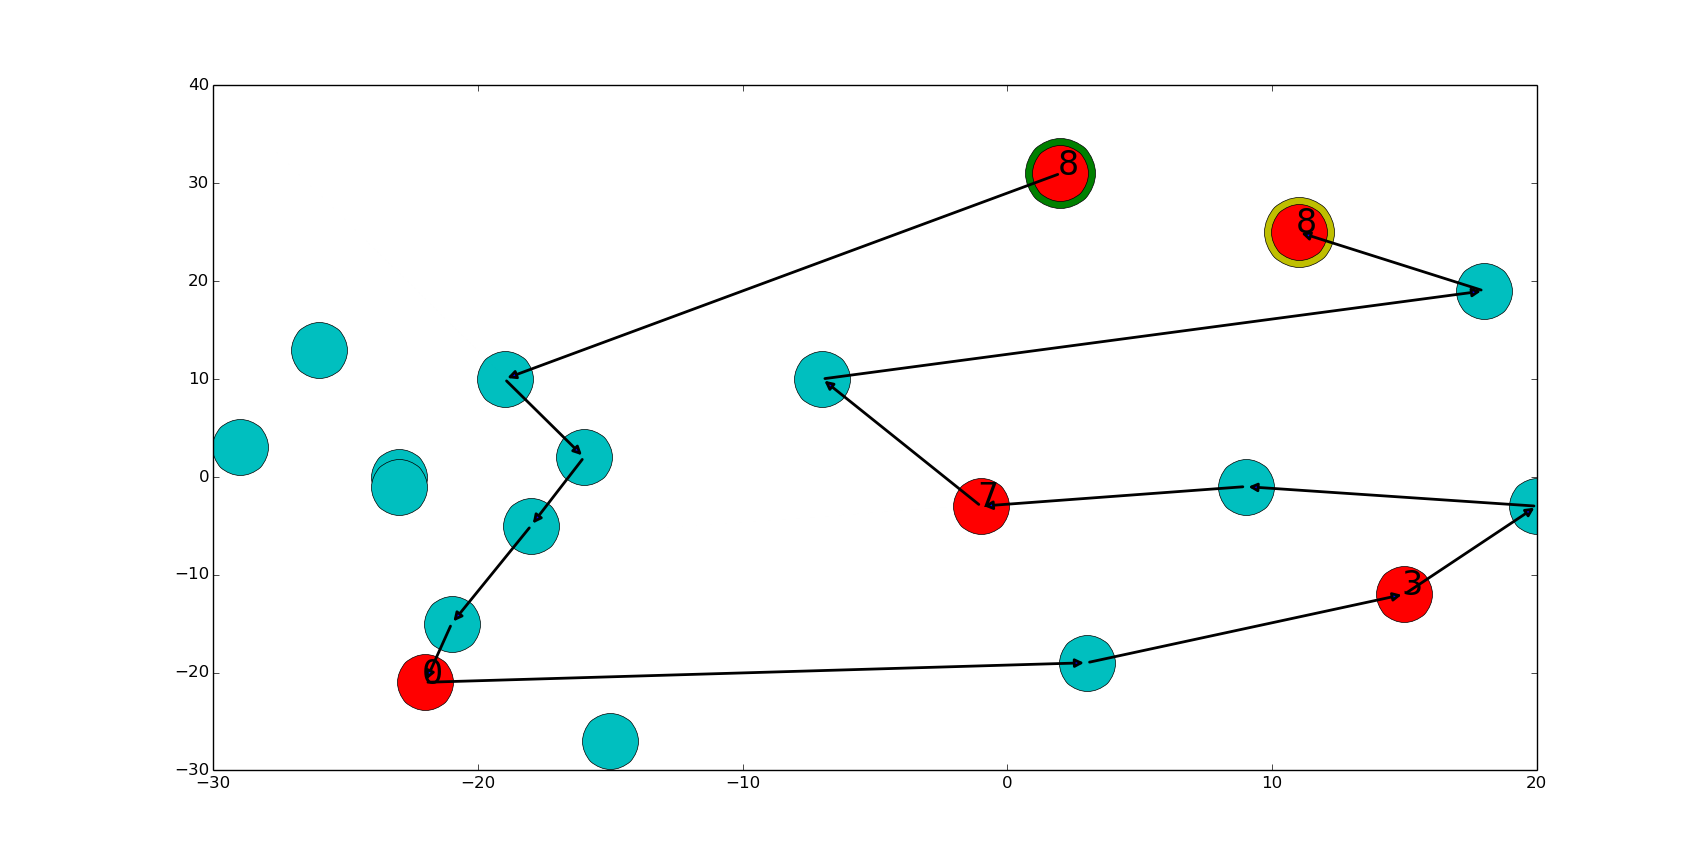
\includegraphics[scale=0.3]{./EJ4/fam82opt.png}\\
 {            \textit{Soluci\'on TABU 2-OPT}}
  \end{center}
  \vspace*{0.3cm}

\vspace*{0.3cm} \vspace*{0.3cm}
  \begin{center}
 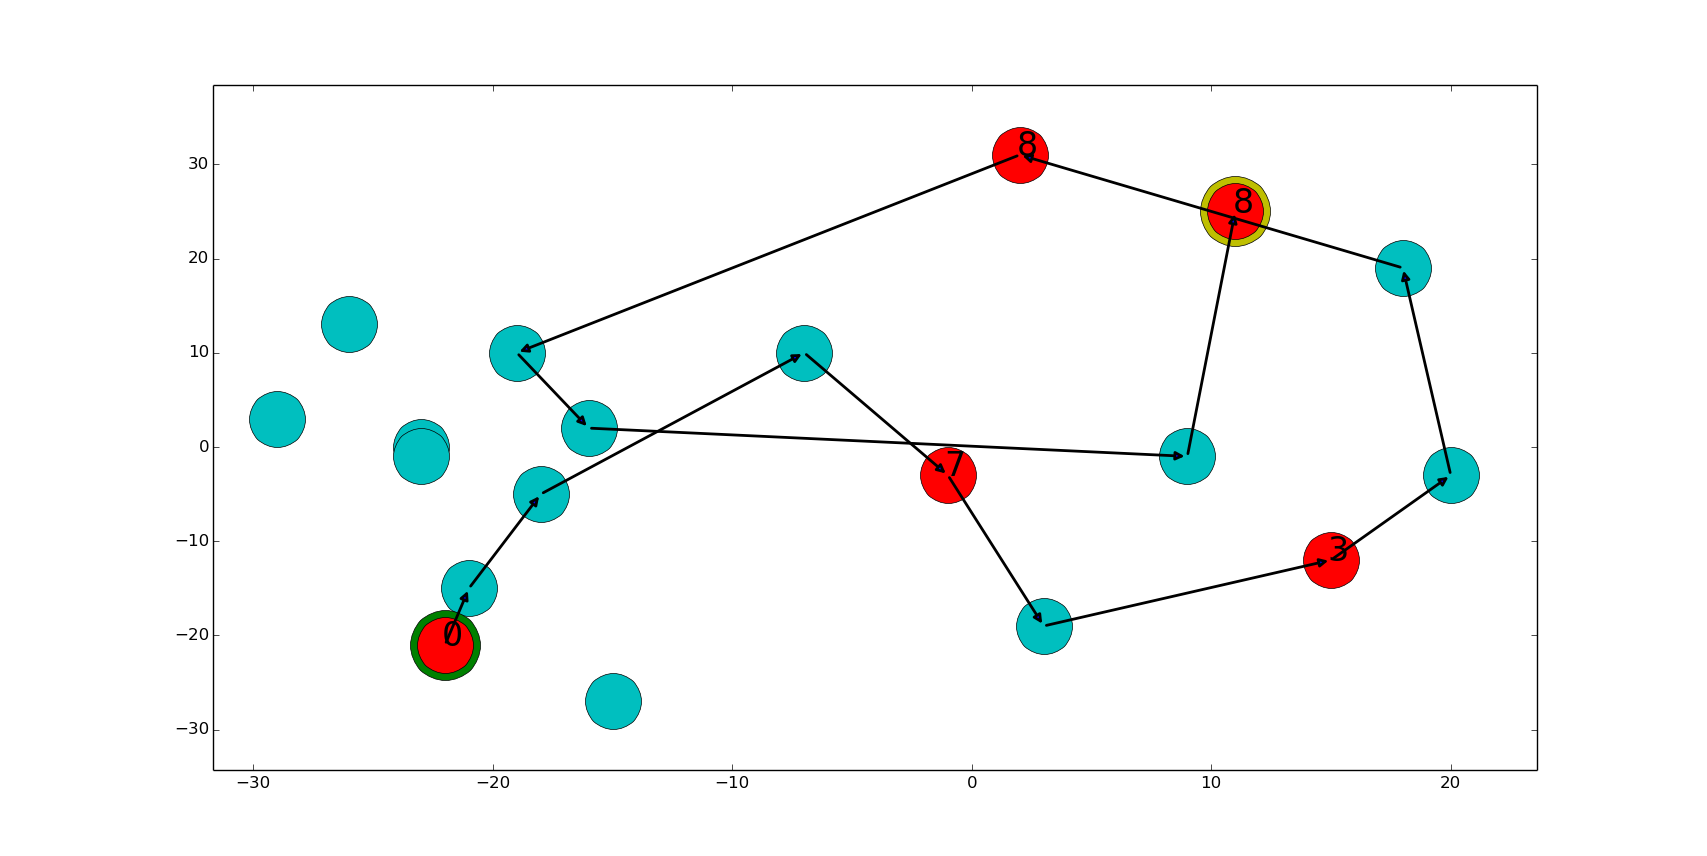
\includegraphics[scale=0.3]{./EJ4/fam83opt.png}\\
 {            \textit{Soluci\'on TABU 3-OPT}}
  \end{center}
  \vspace*{0.3cm}

Veamos como se comporta Tabu 2-OPT con respecto a la heuristica de busqueda local 2-OPT:

\vspace*{0.3cm} \vspace*{0.3cm}
  \begin{center}
 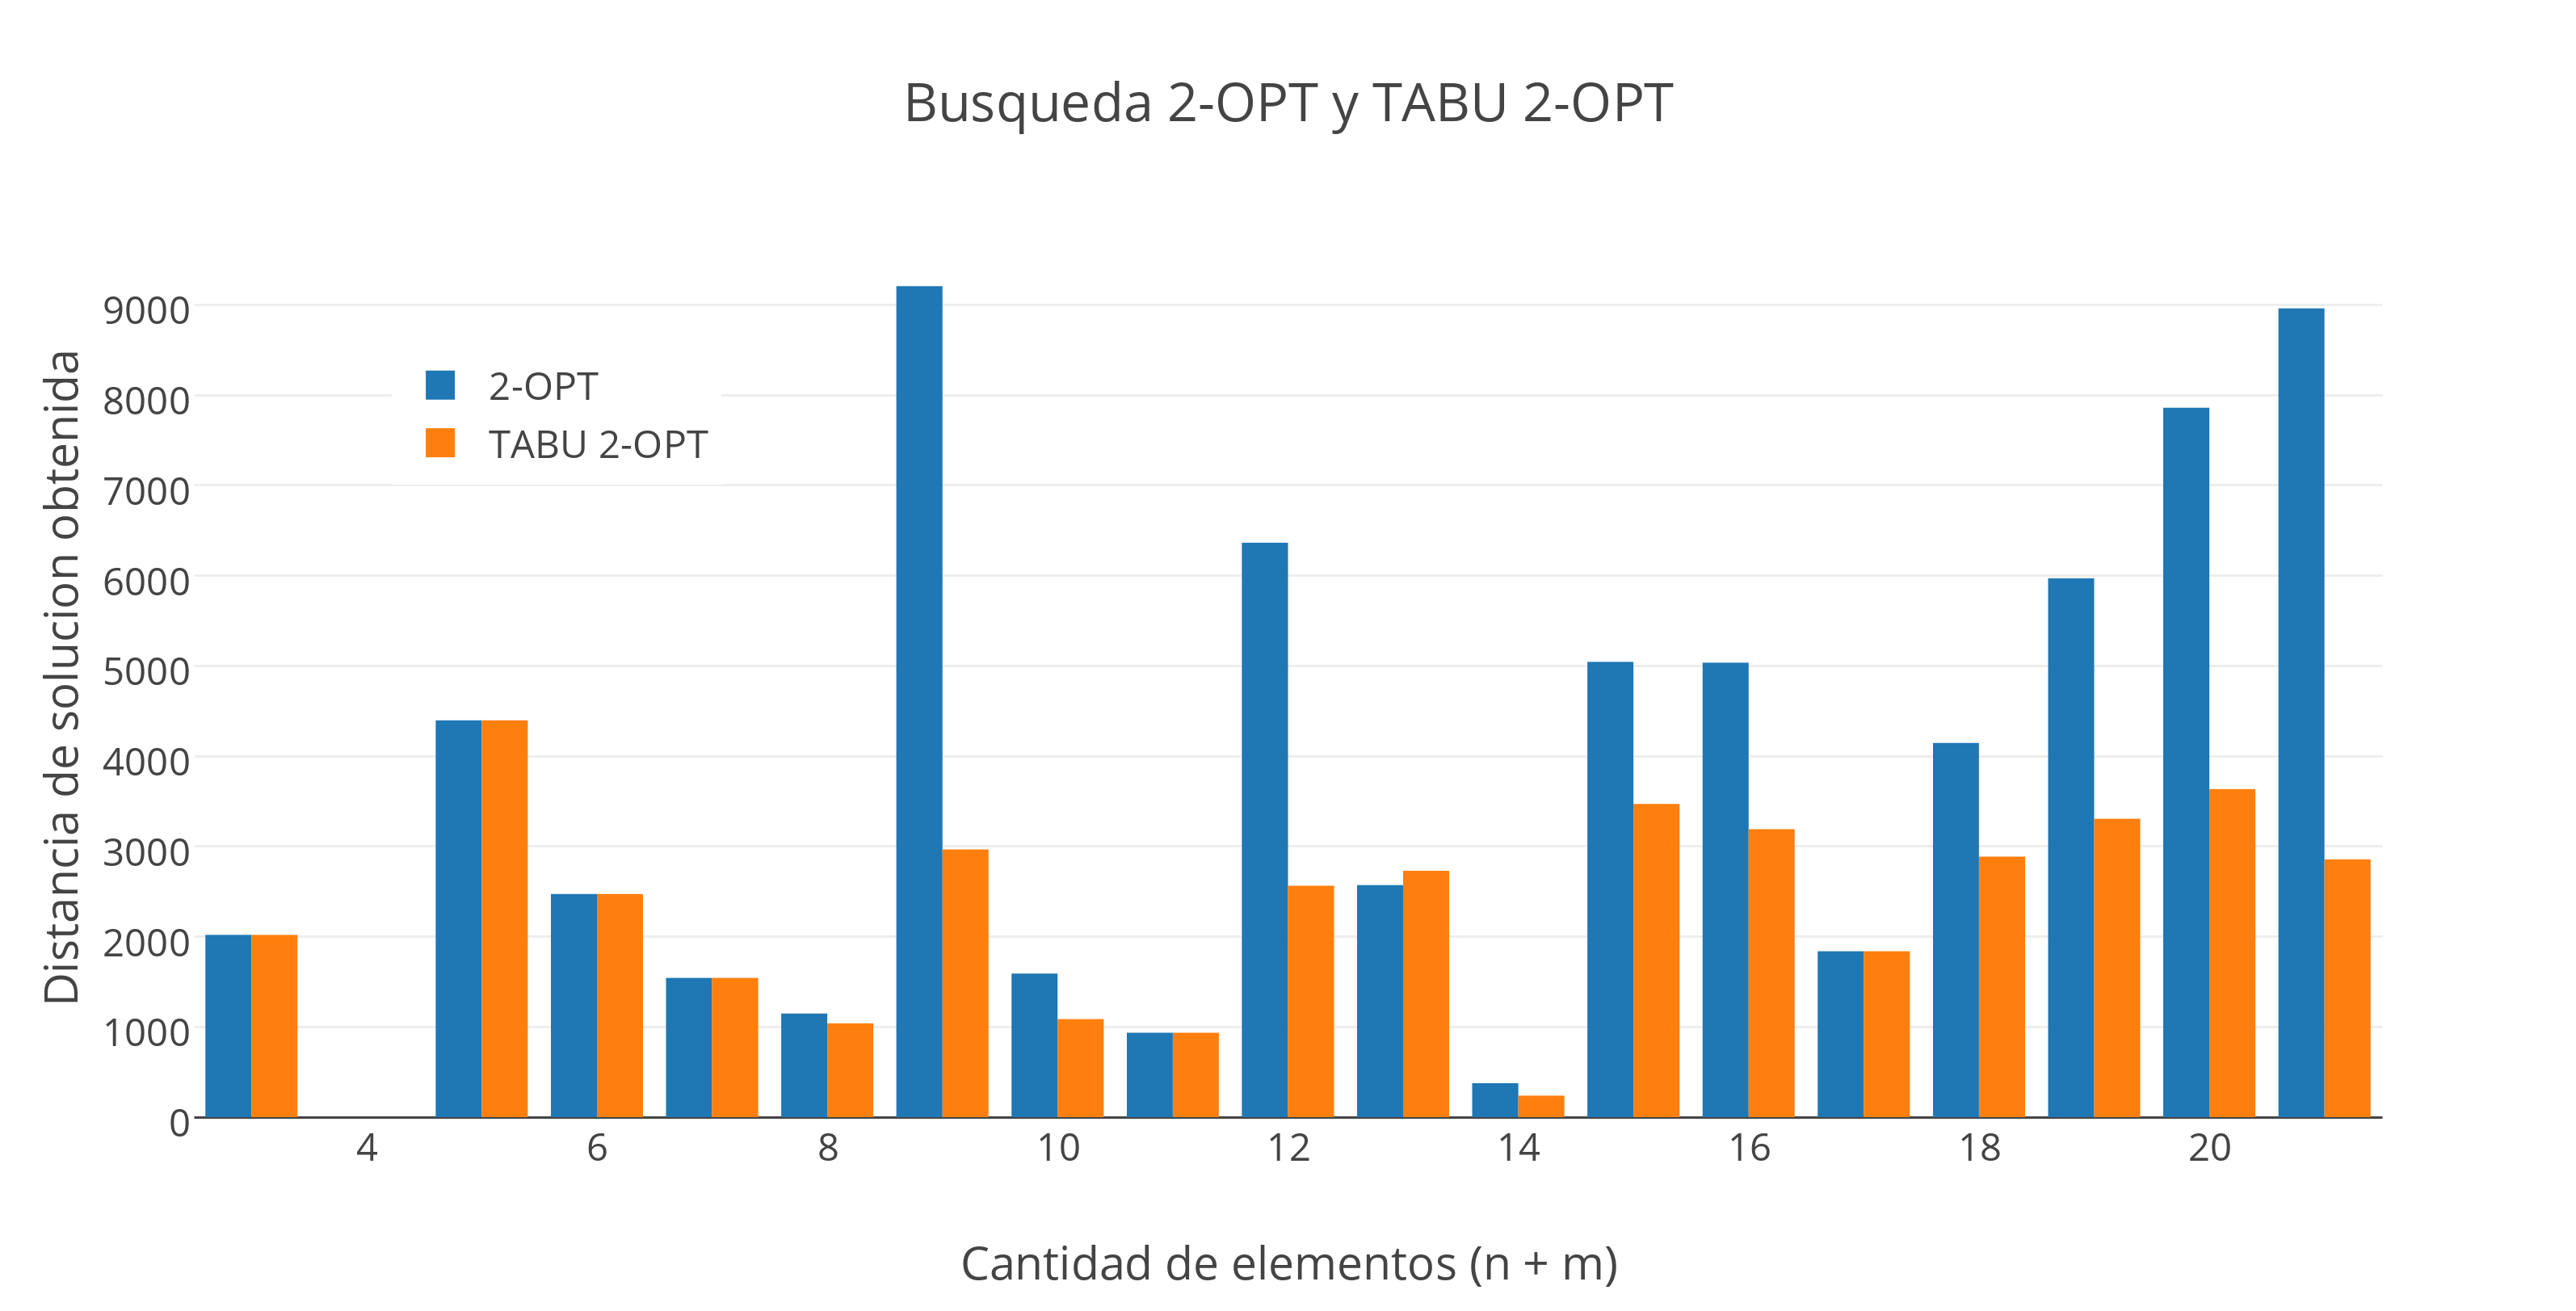
\includegraphics[scale=0.5]{./EJ4/comparativorandom2opt.png}\\
 {            \textit{Gráfico \ 4.7 - 2-OPT vs Tabu 2-OPT sobre Familia 8}}
  \end{center}
  \vspace*{0.3cm}

\vspace*{0.3cm} \vspace*{0.3cm}
  \begin{center}
 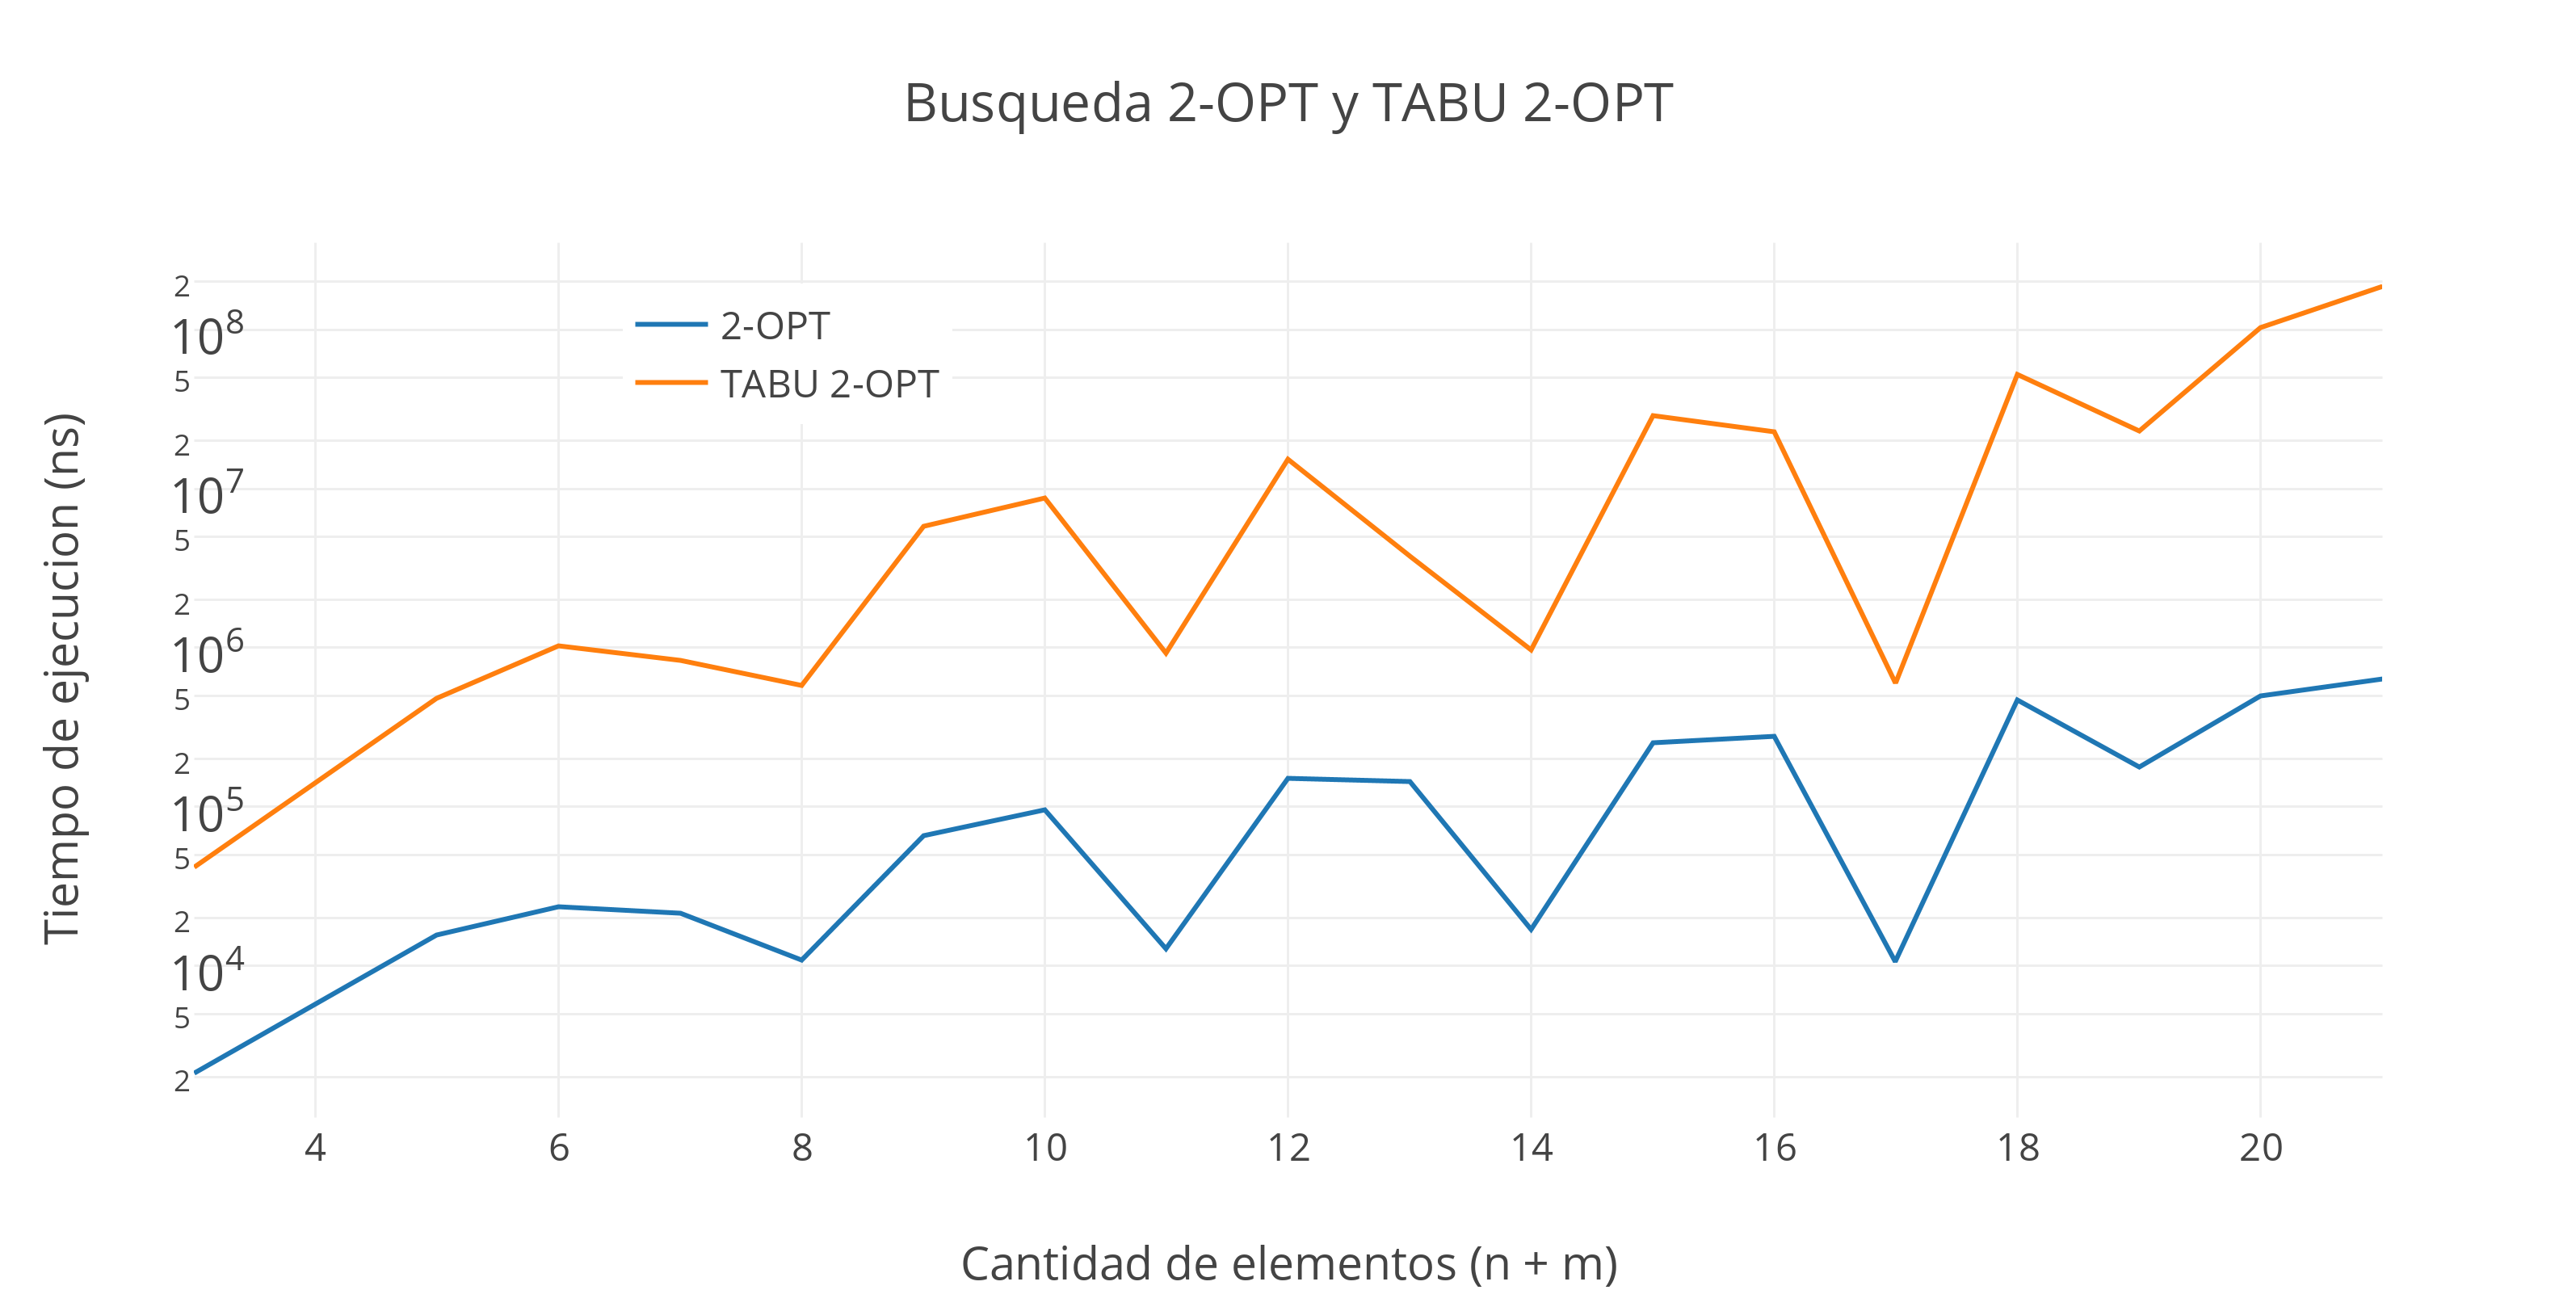
\includegraphics[scale=0.5]{./EJ4/medicionrandom2opt.png}\\
 {            \textit{Gráfico \ 4.8 - 2-OPT vs Tabu 2-OPT sobre Familia 6}}
  \end{center}
  \vspace*{0.3cm}

Luego, para 3-OPT:

\vspace*{0.3cm} \vspace*{0.3cm}
  \begin{center}
 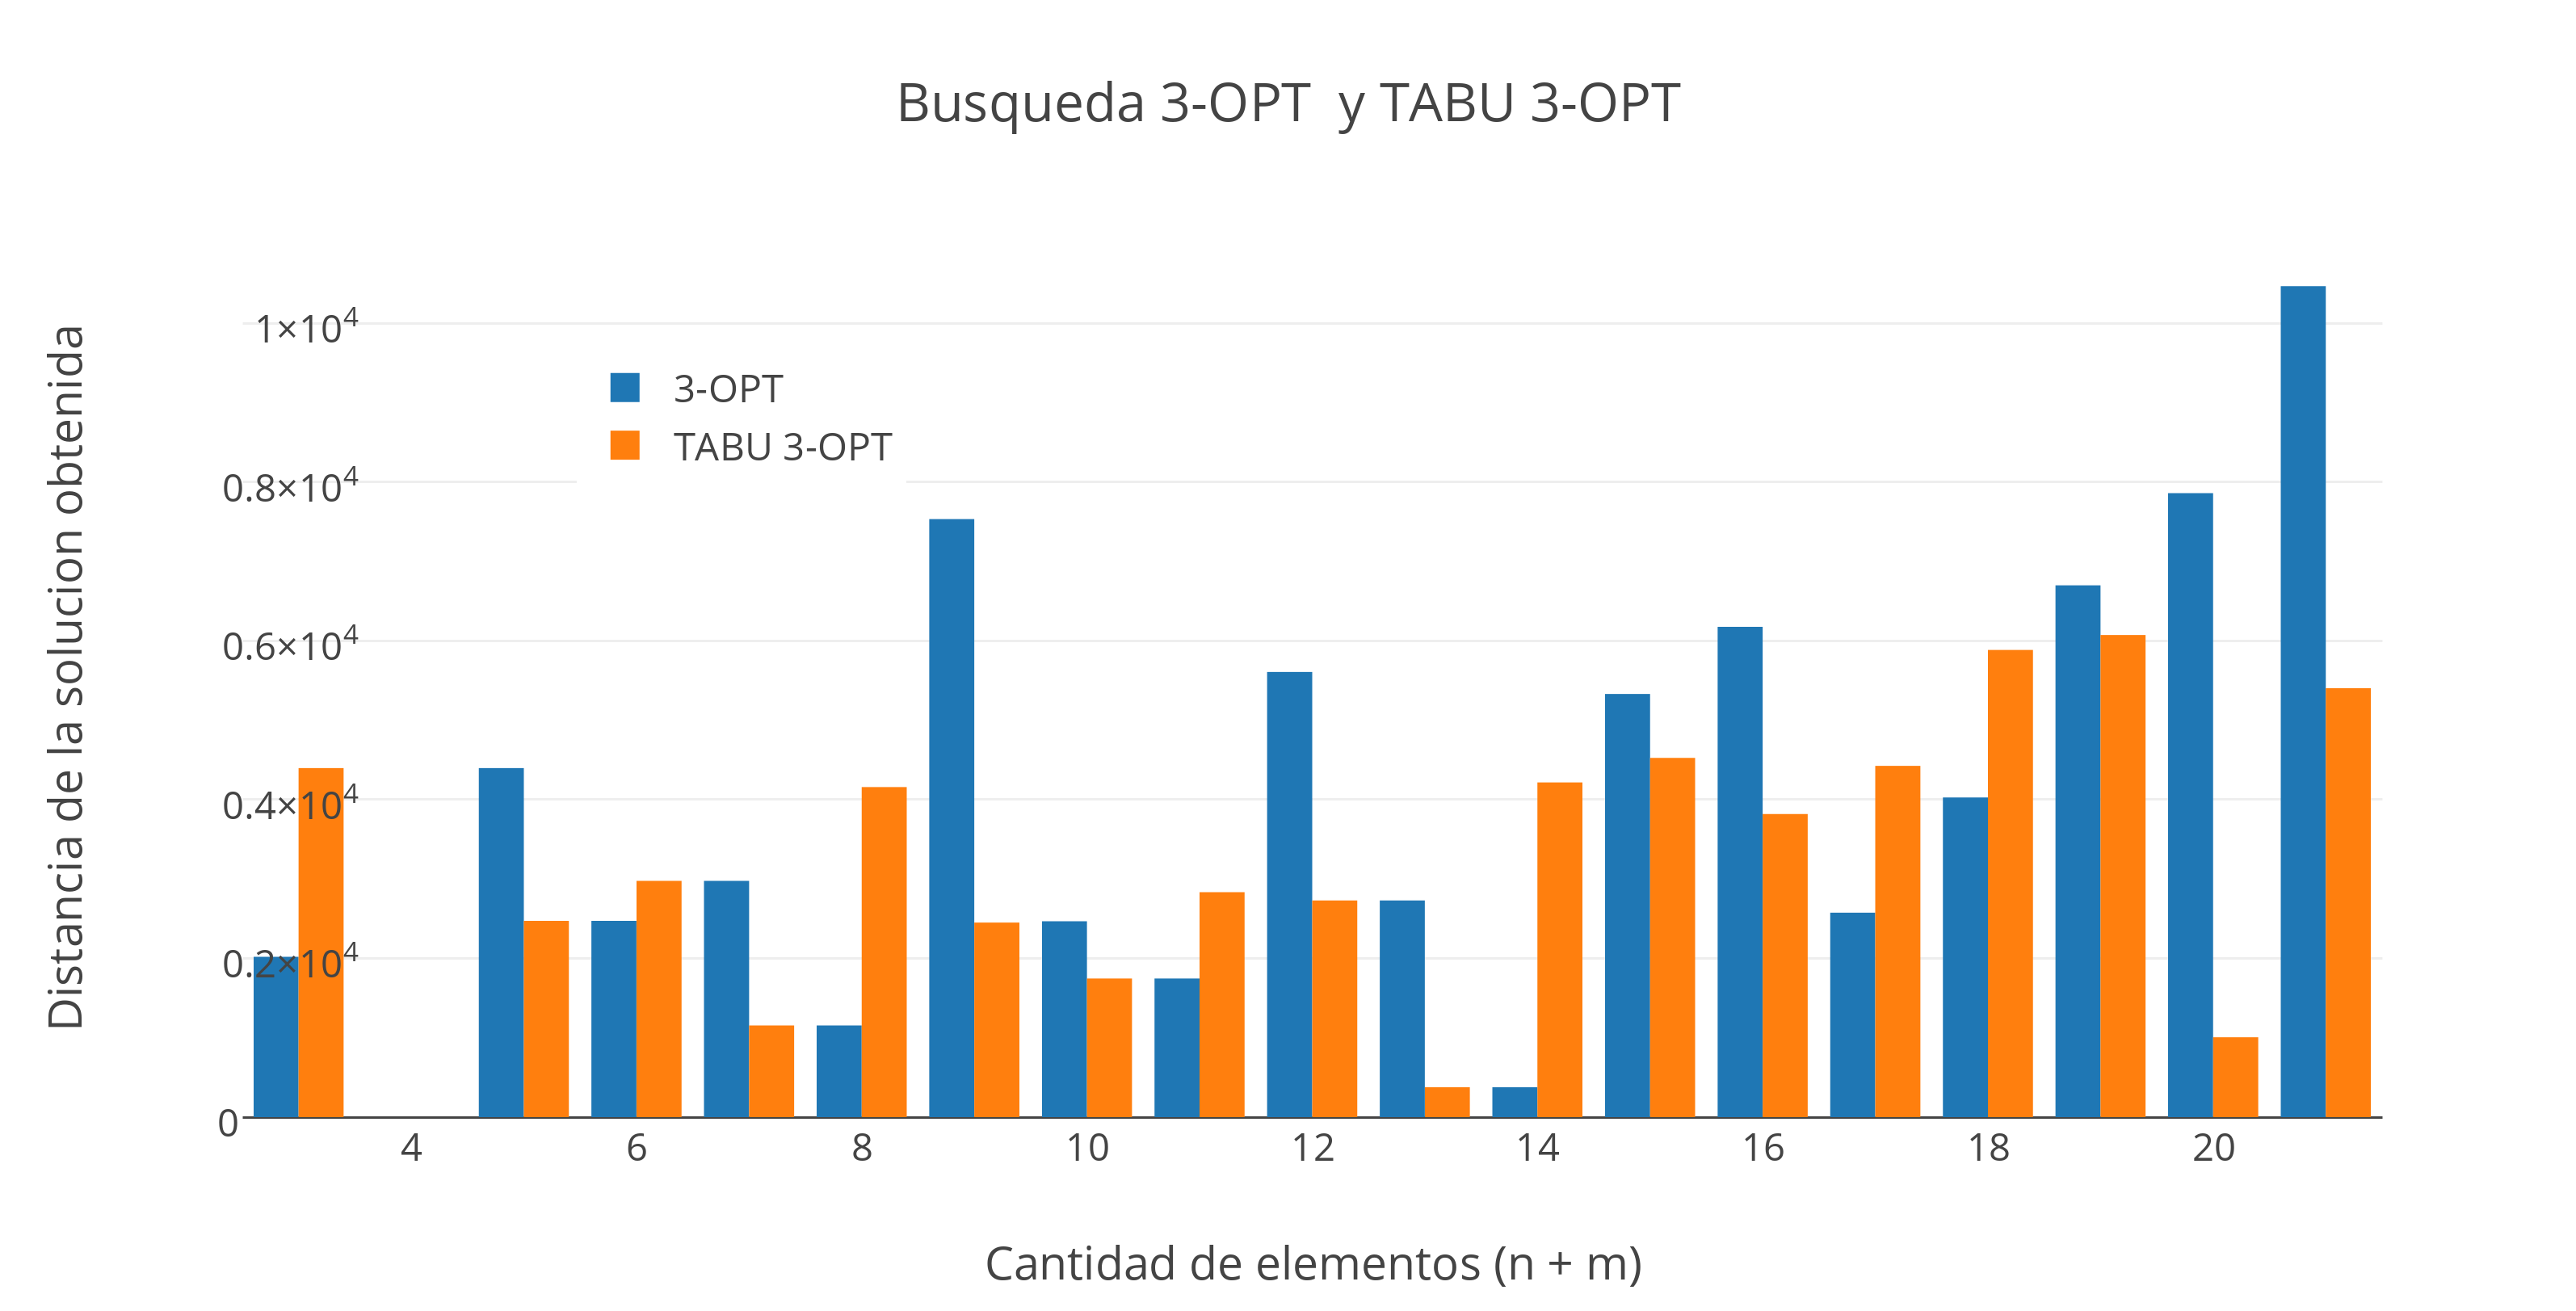
\includegraphics[scale=0.5]{./EJ4/comparativorandom3opt.png}\\
 {            \textit{Gráfico \ 4.9 - 3-OPT vs Tabu 3-OPT sobre Familia 6}}
  \end{center}
  \vspace*{0.3cm}

\vspace*{0.3cm} \vspace*{0.3cm}
  \begin{center}
 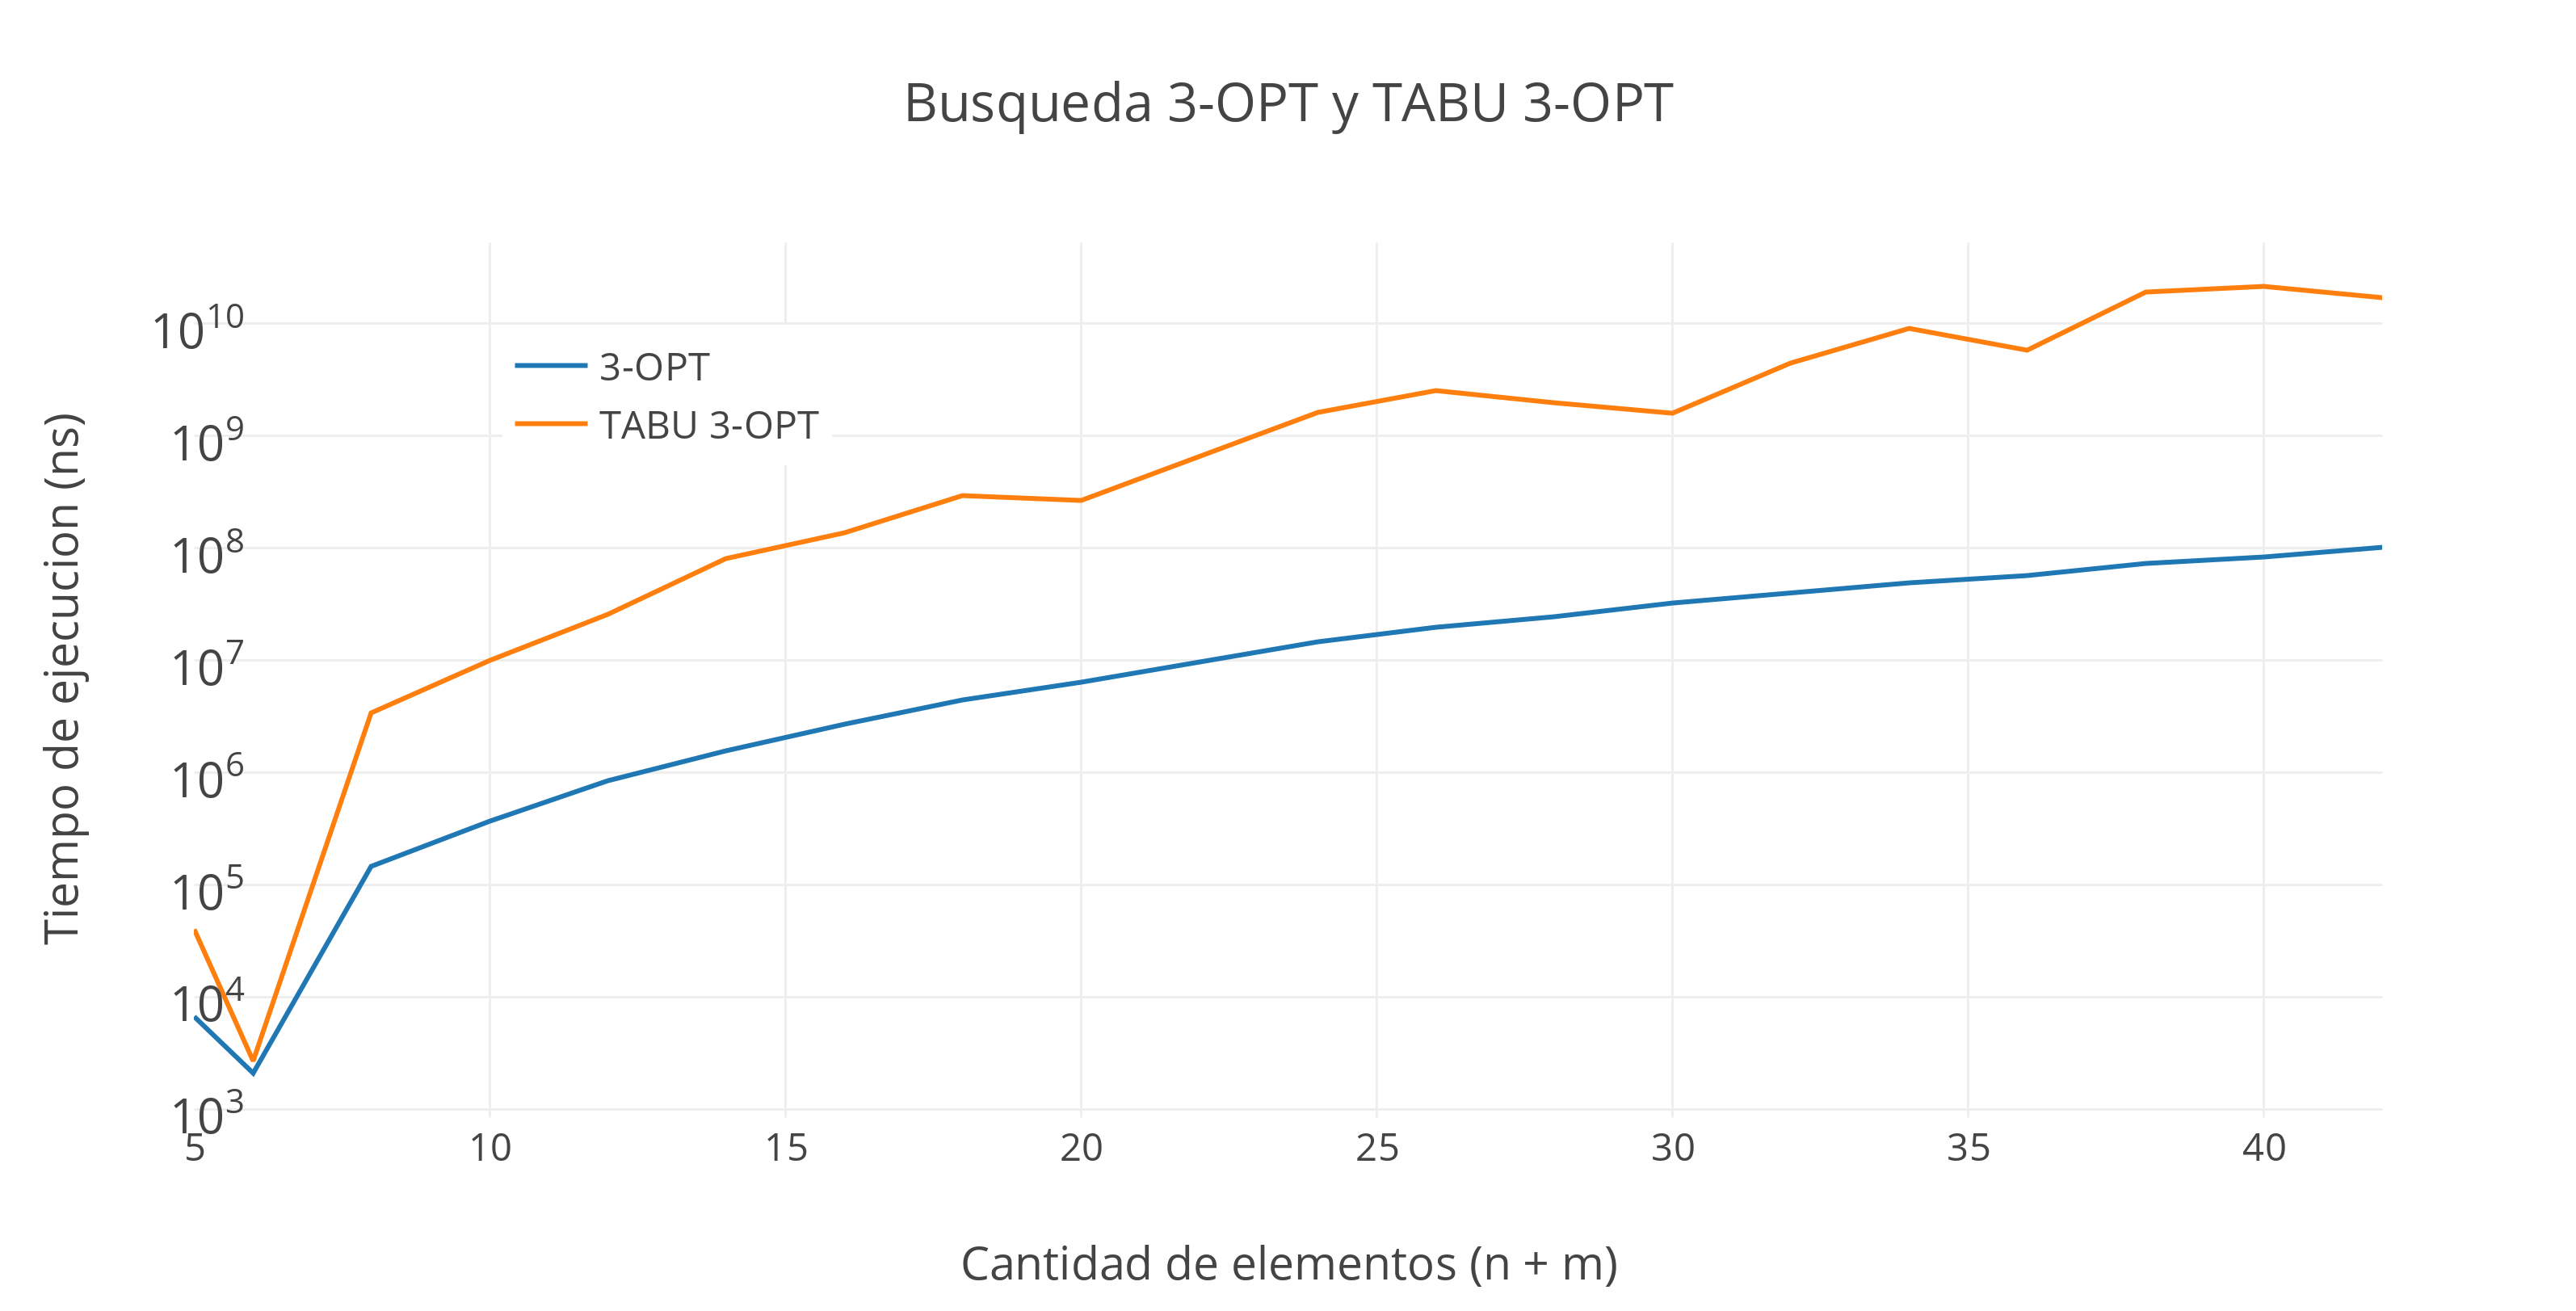
\includegraphics[scale=0.5]{./EJ4/medicionrandom3opt.png}\\
 {            \textit{Gráfico \ 4.10 - 3-OPT vs Tabu 3-OPT sobre Familia 6}}
  \end{center}
  \vspace*{0.3cm}
  
--> OBTENER CONCLUSIONES
  
Comparando las soluciones de cada version de tabú search podemos observar lo siguiente: 

\vspace*{0.3cm} \vspace*{0.3cm}
  \begin{center}
 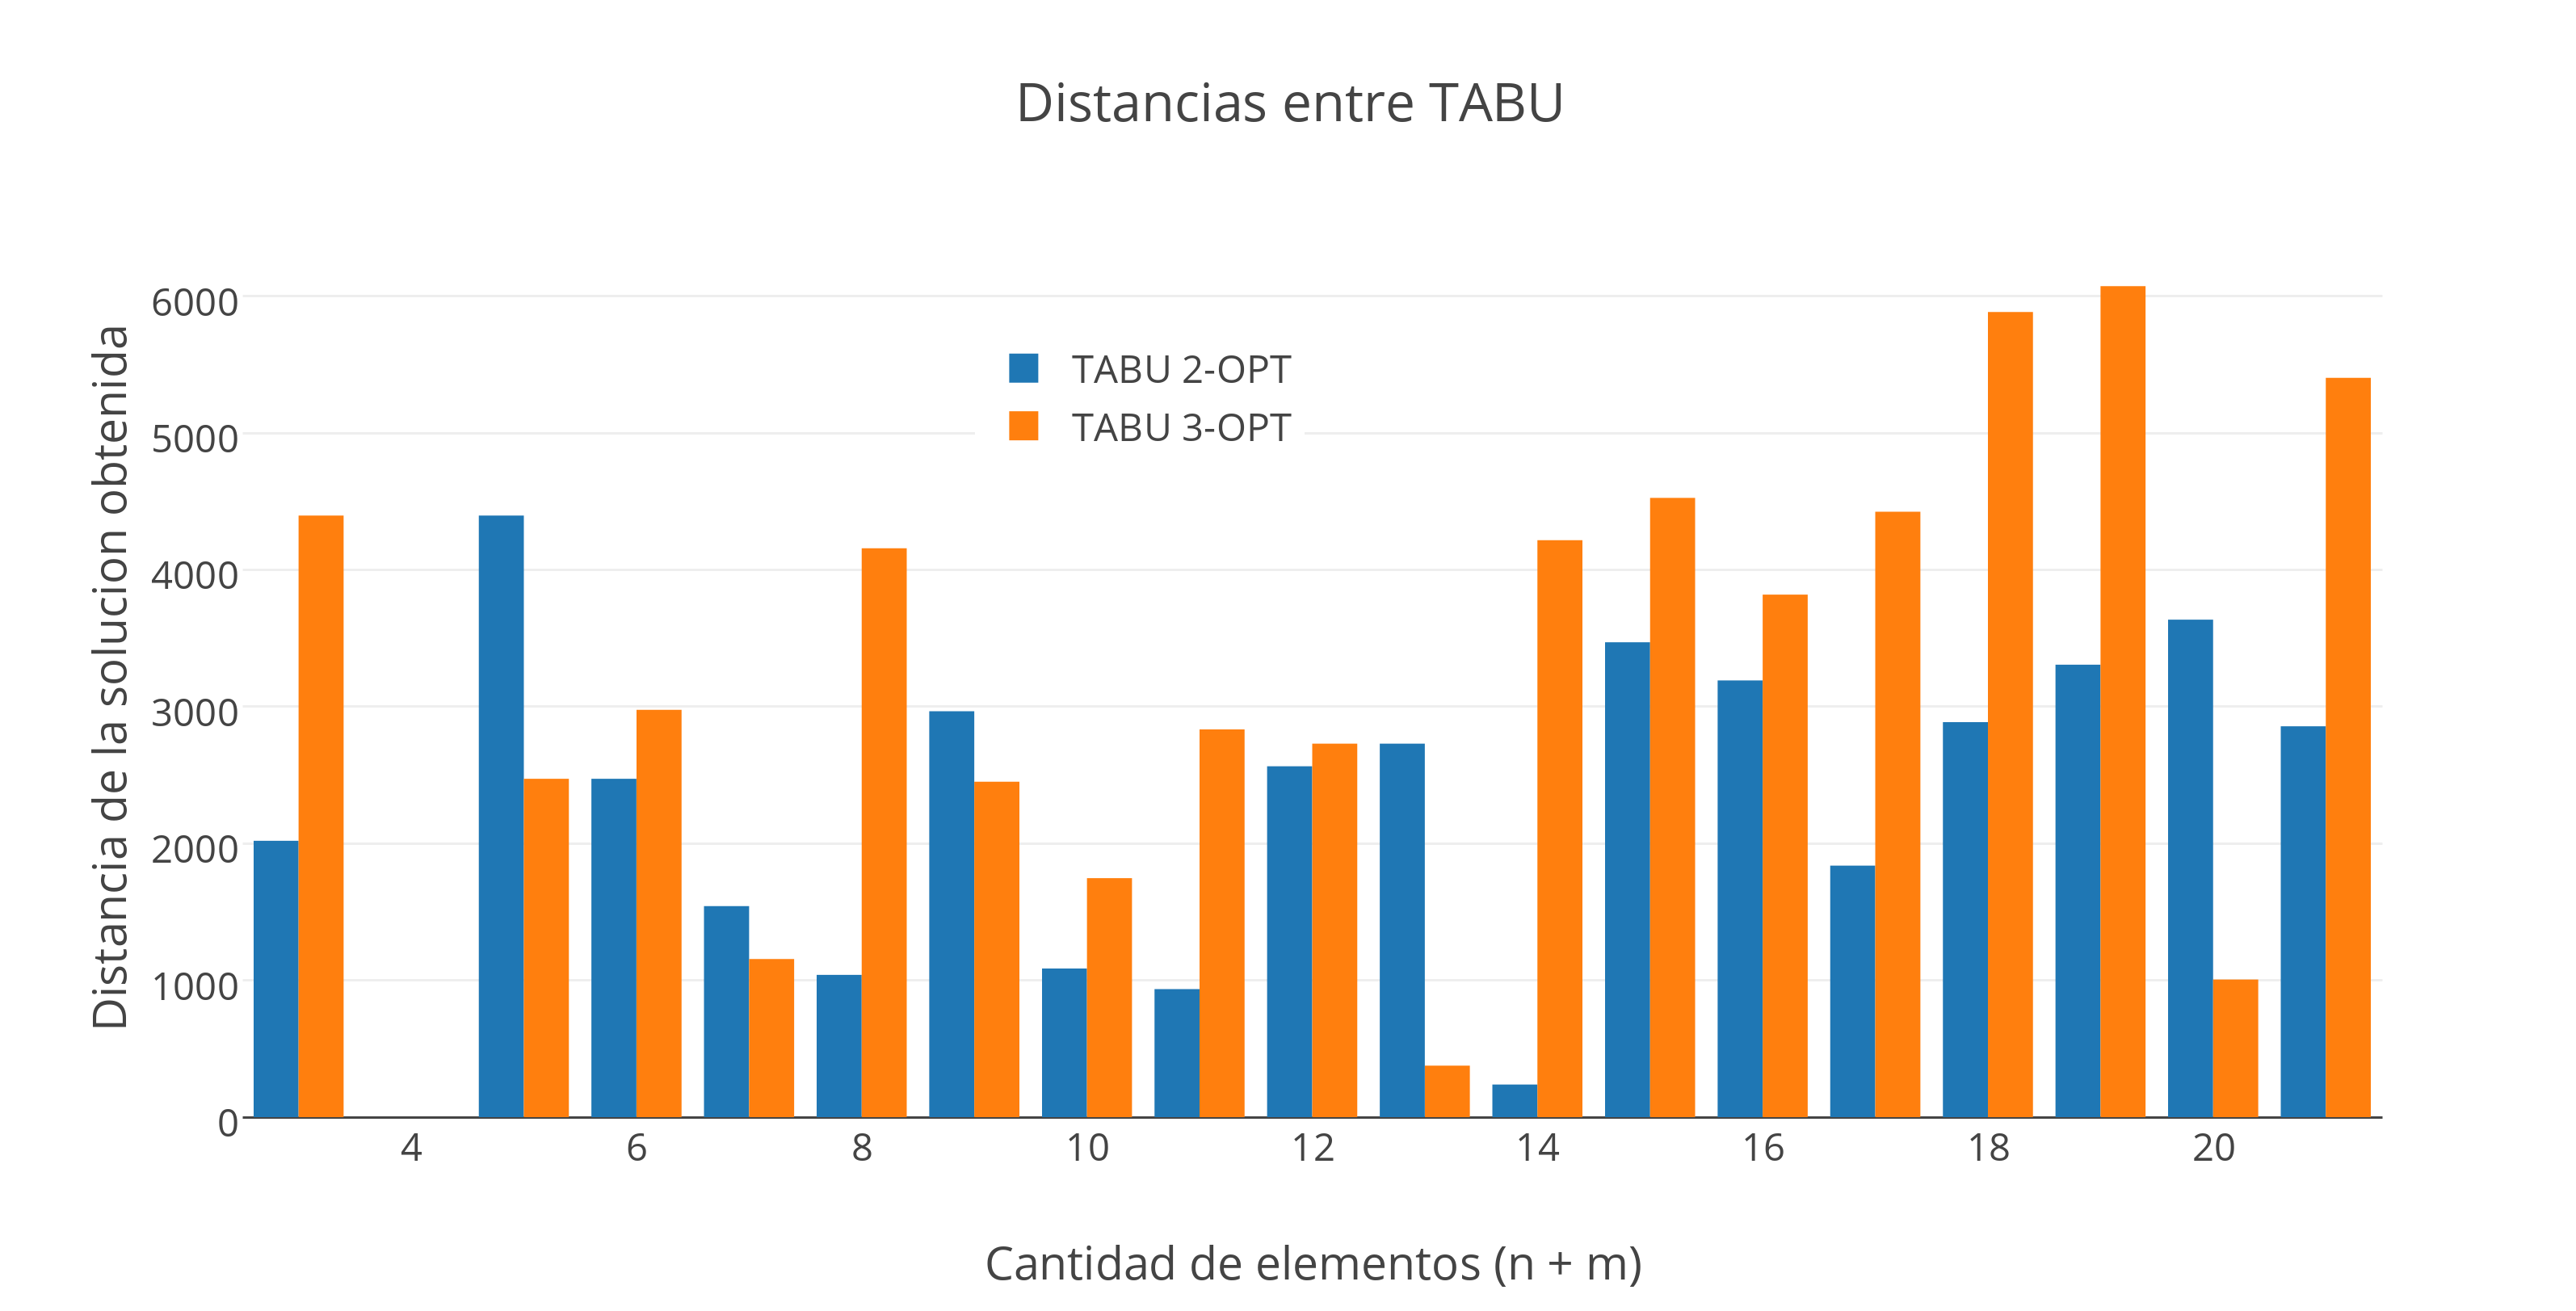
\includegraphics[scale=0.5]{./EJ4/comparativorandom.png}\\
 {            \textit{Gráfico \ 4.11 - Tabu 2-OPT vs Tabu 3-OPT sobre Familia 6}}
  \end{center}
  \vspace*{0.3cm}

\vspace*{0.3cm} \vspace*{0.3cm}
  \begin{center}
 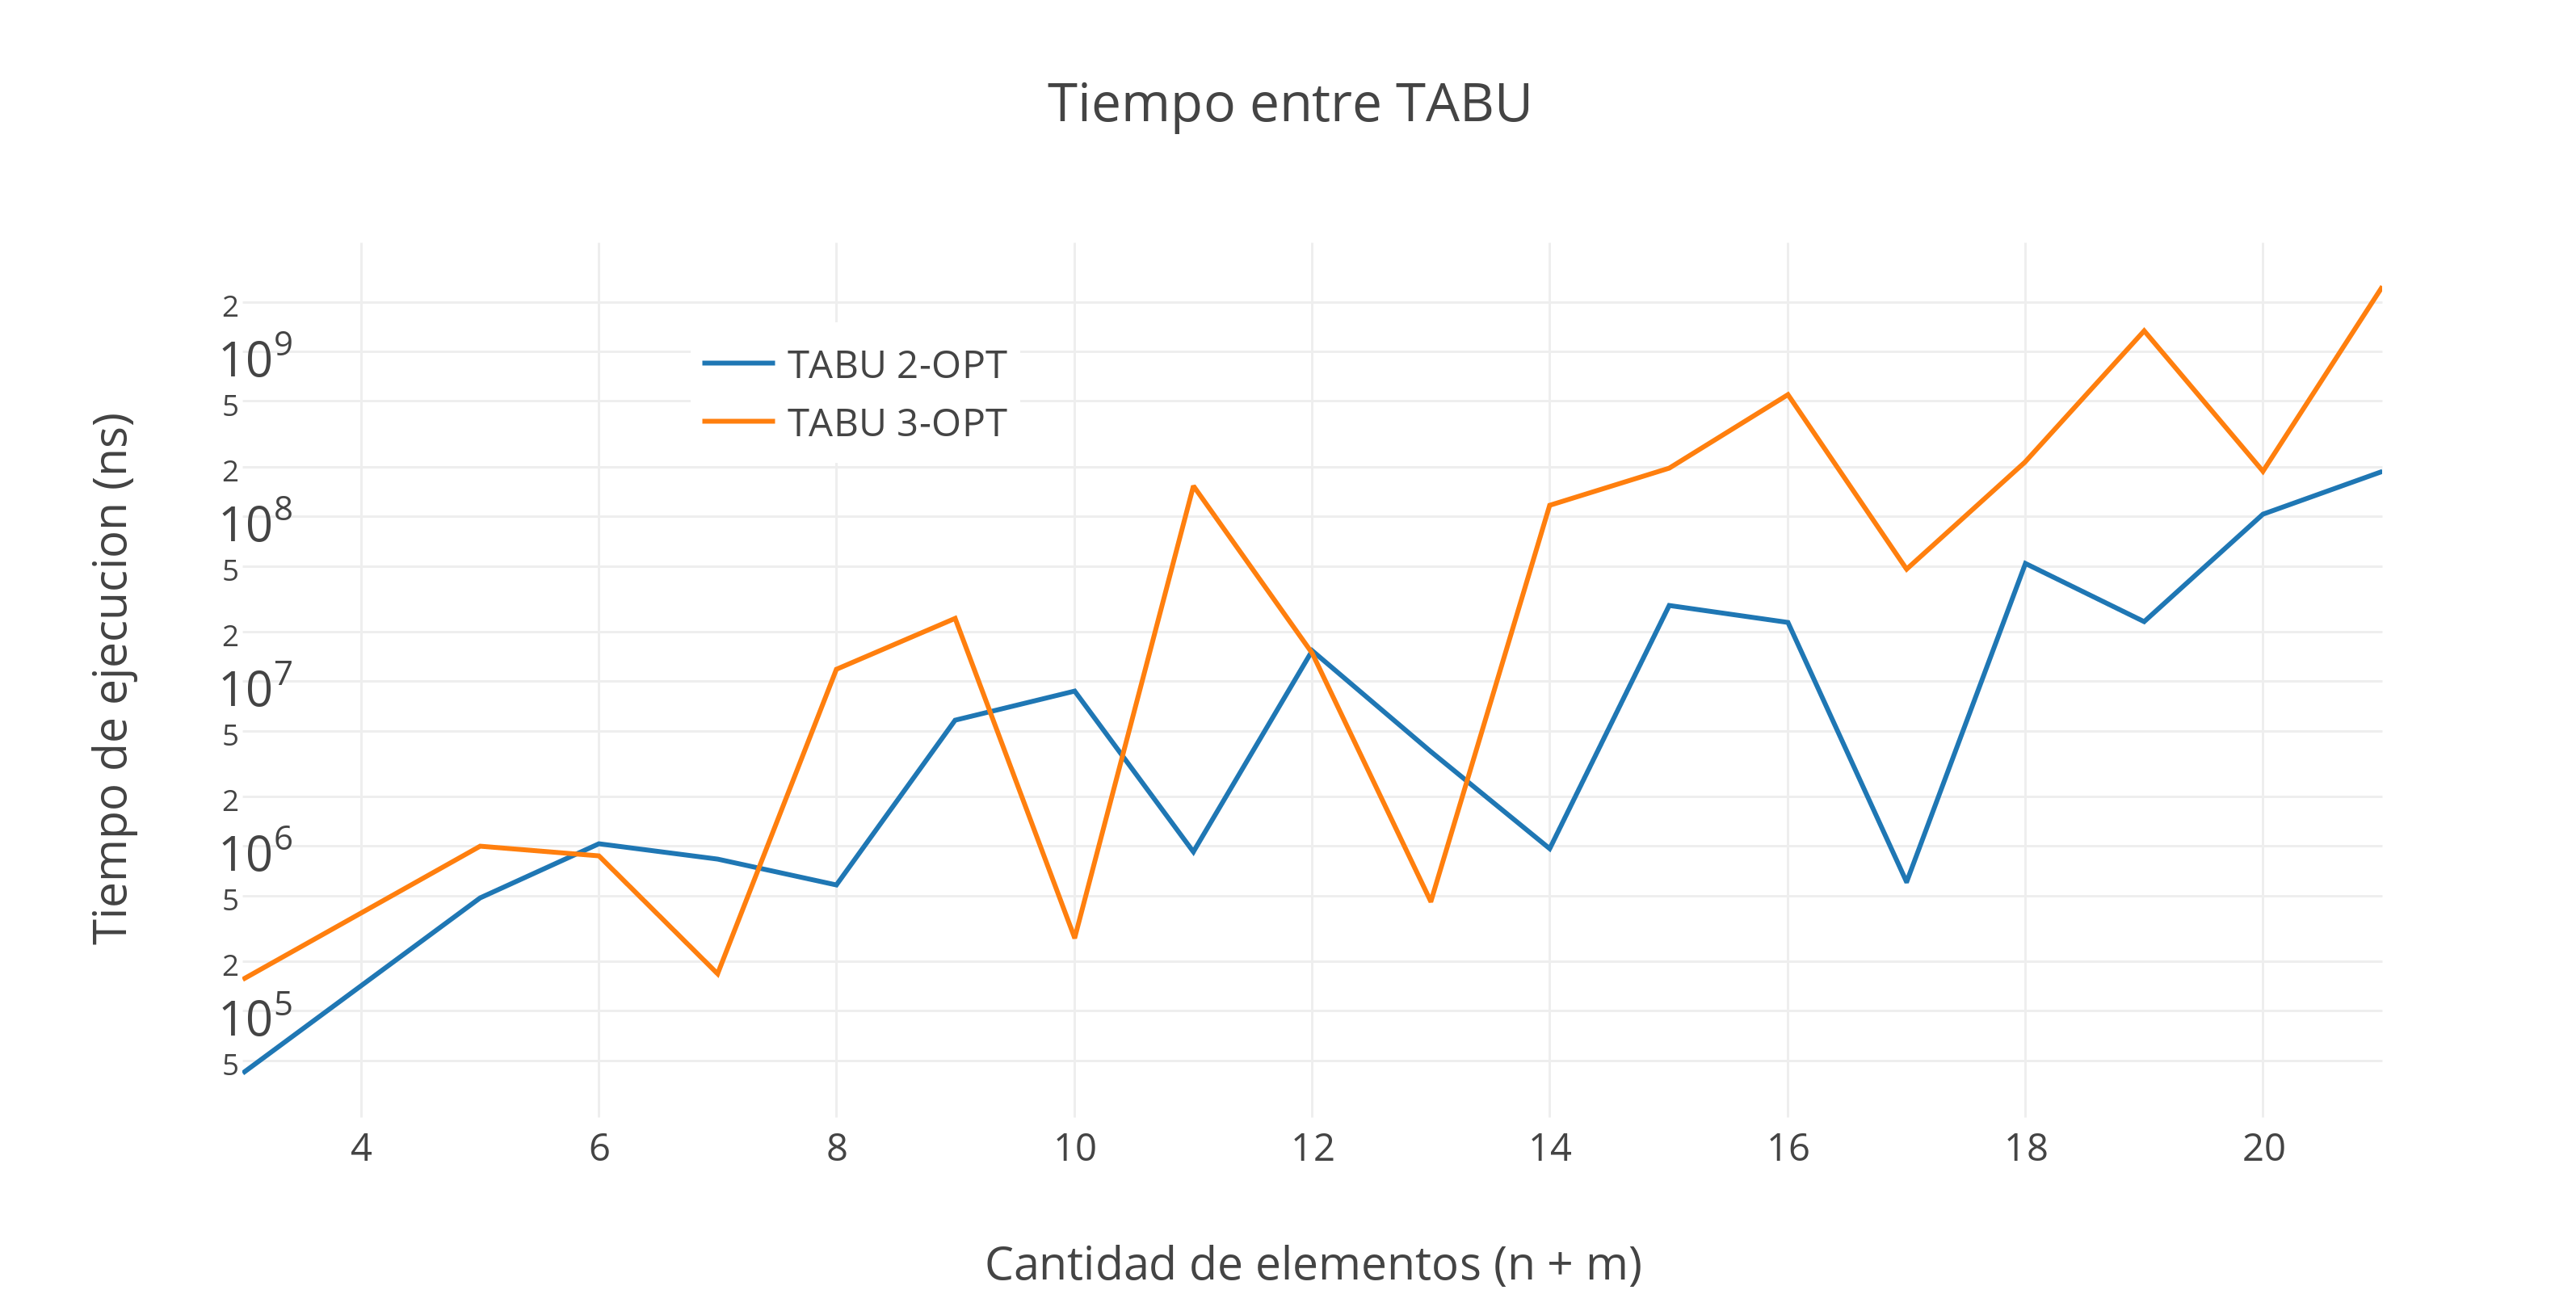
\includegraphics[scale=0.5]{./EJ4/medicionrandom.png}\\
 {            \textit{Gráfico \ 4.12 - Tabu 2-OPT vs Tabu 3-OPT sobre Familia 6}}
  \end{center}
  \vspace*{0.3cm}
  
--> OBTENER CONCLUSIONES

--> OBTENER CONCLUSIONES GENERALES SOBRE ESTOS TESTS: CUAL VERSION DE TABU CONVIENE MAS? EN QUE CASOS CONVIENE HACER BUSQUEDA LOCAL UNICAMENTE?  
  
--> ANALISIS DEL TRADE OFF: sobre la cantidad de iteraciones y la condicion de corte por producirse limite de no mejoras

\vspace*{0.3cm} \vspace*{0.3cm}
  \begin{center}
 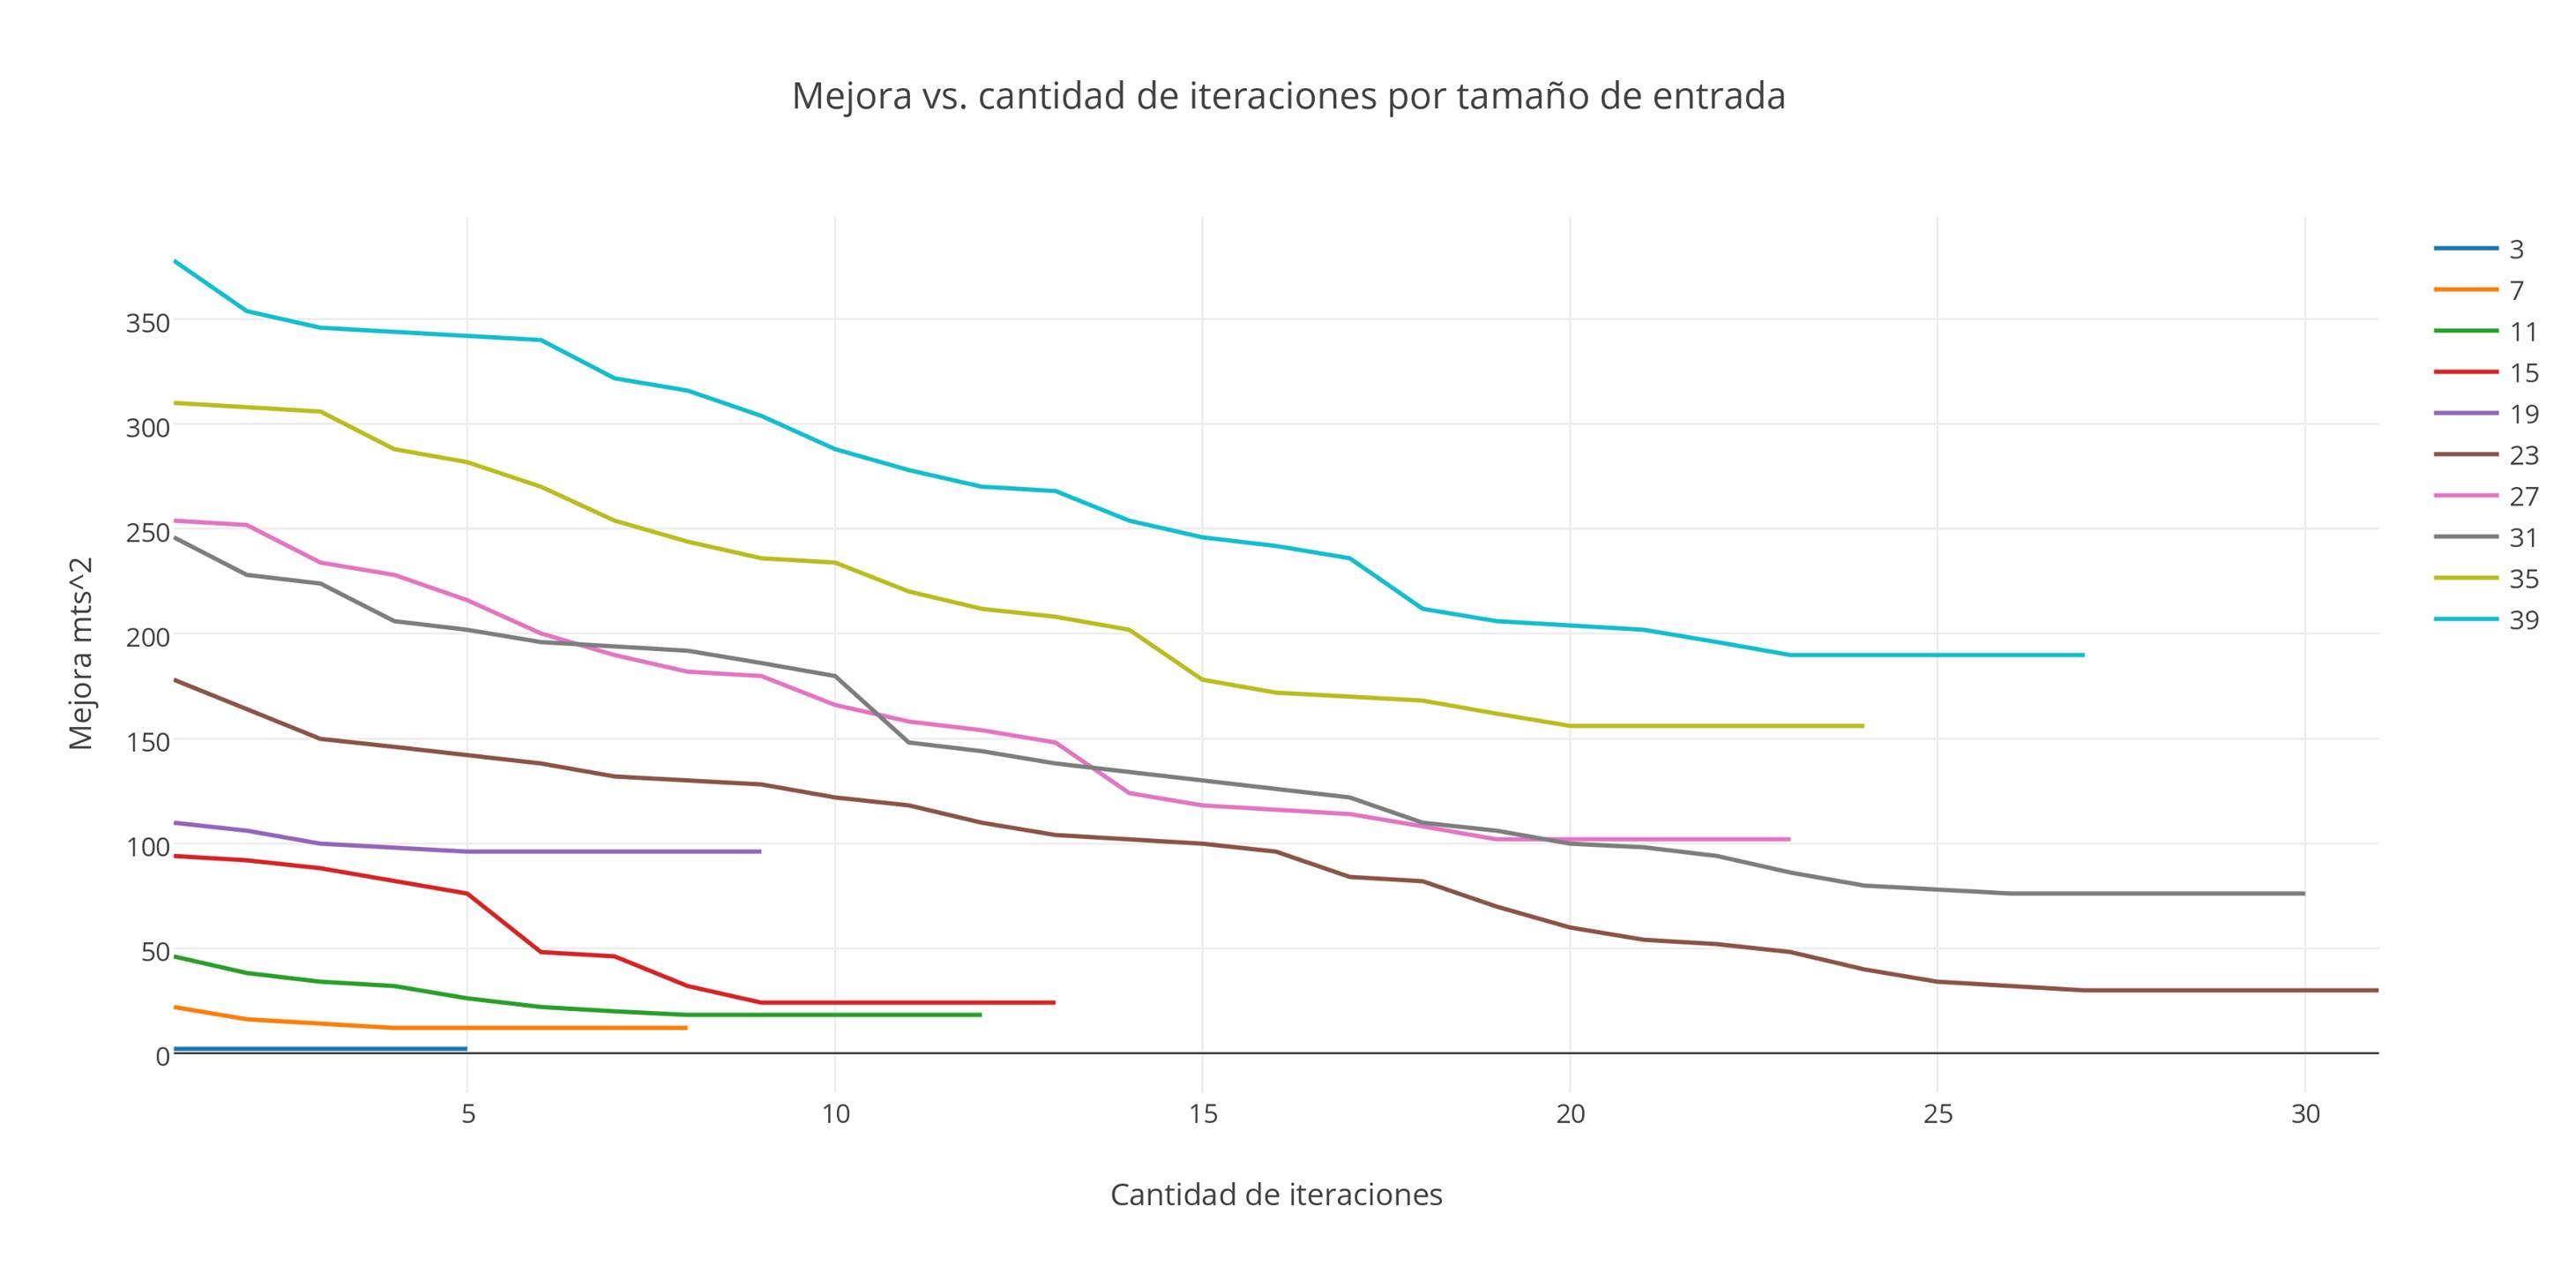
\includegraphics[scale=0.5]{./EJ4/mejora.png}\\
 {            \textit{Gráfico \ 4.12 - Tabu 2-OPT vs Tabu 3-OPT sobre Familia 6}}
  \end{center}
  \vspace*{0.3cm}
  
  \vspace*{0.3cm} \vspace*{0.3cm}
  \begin{center}
 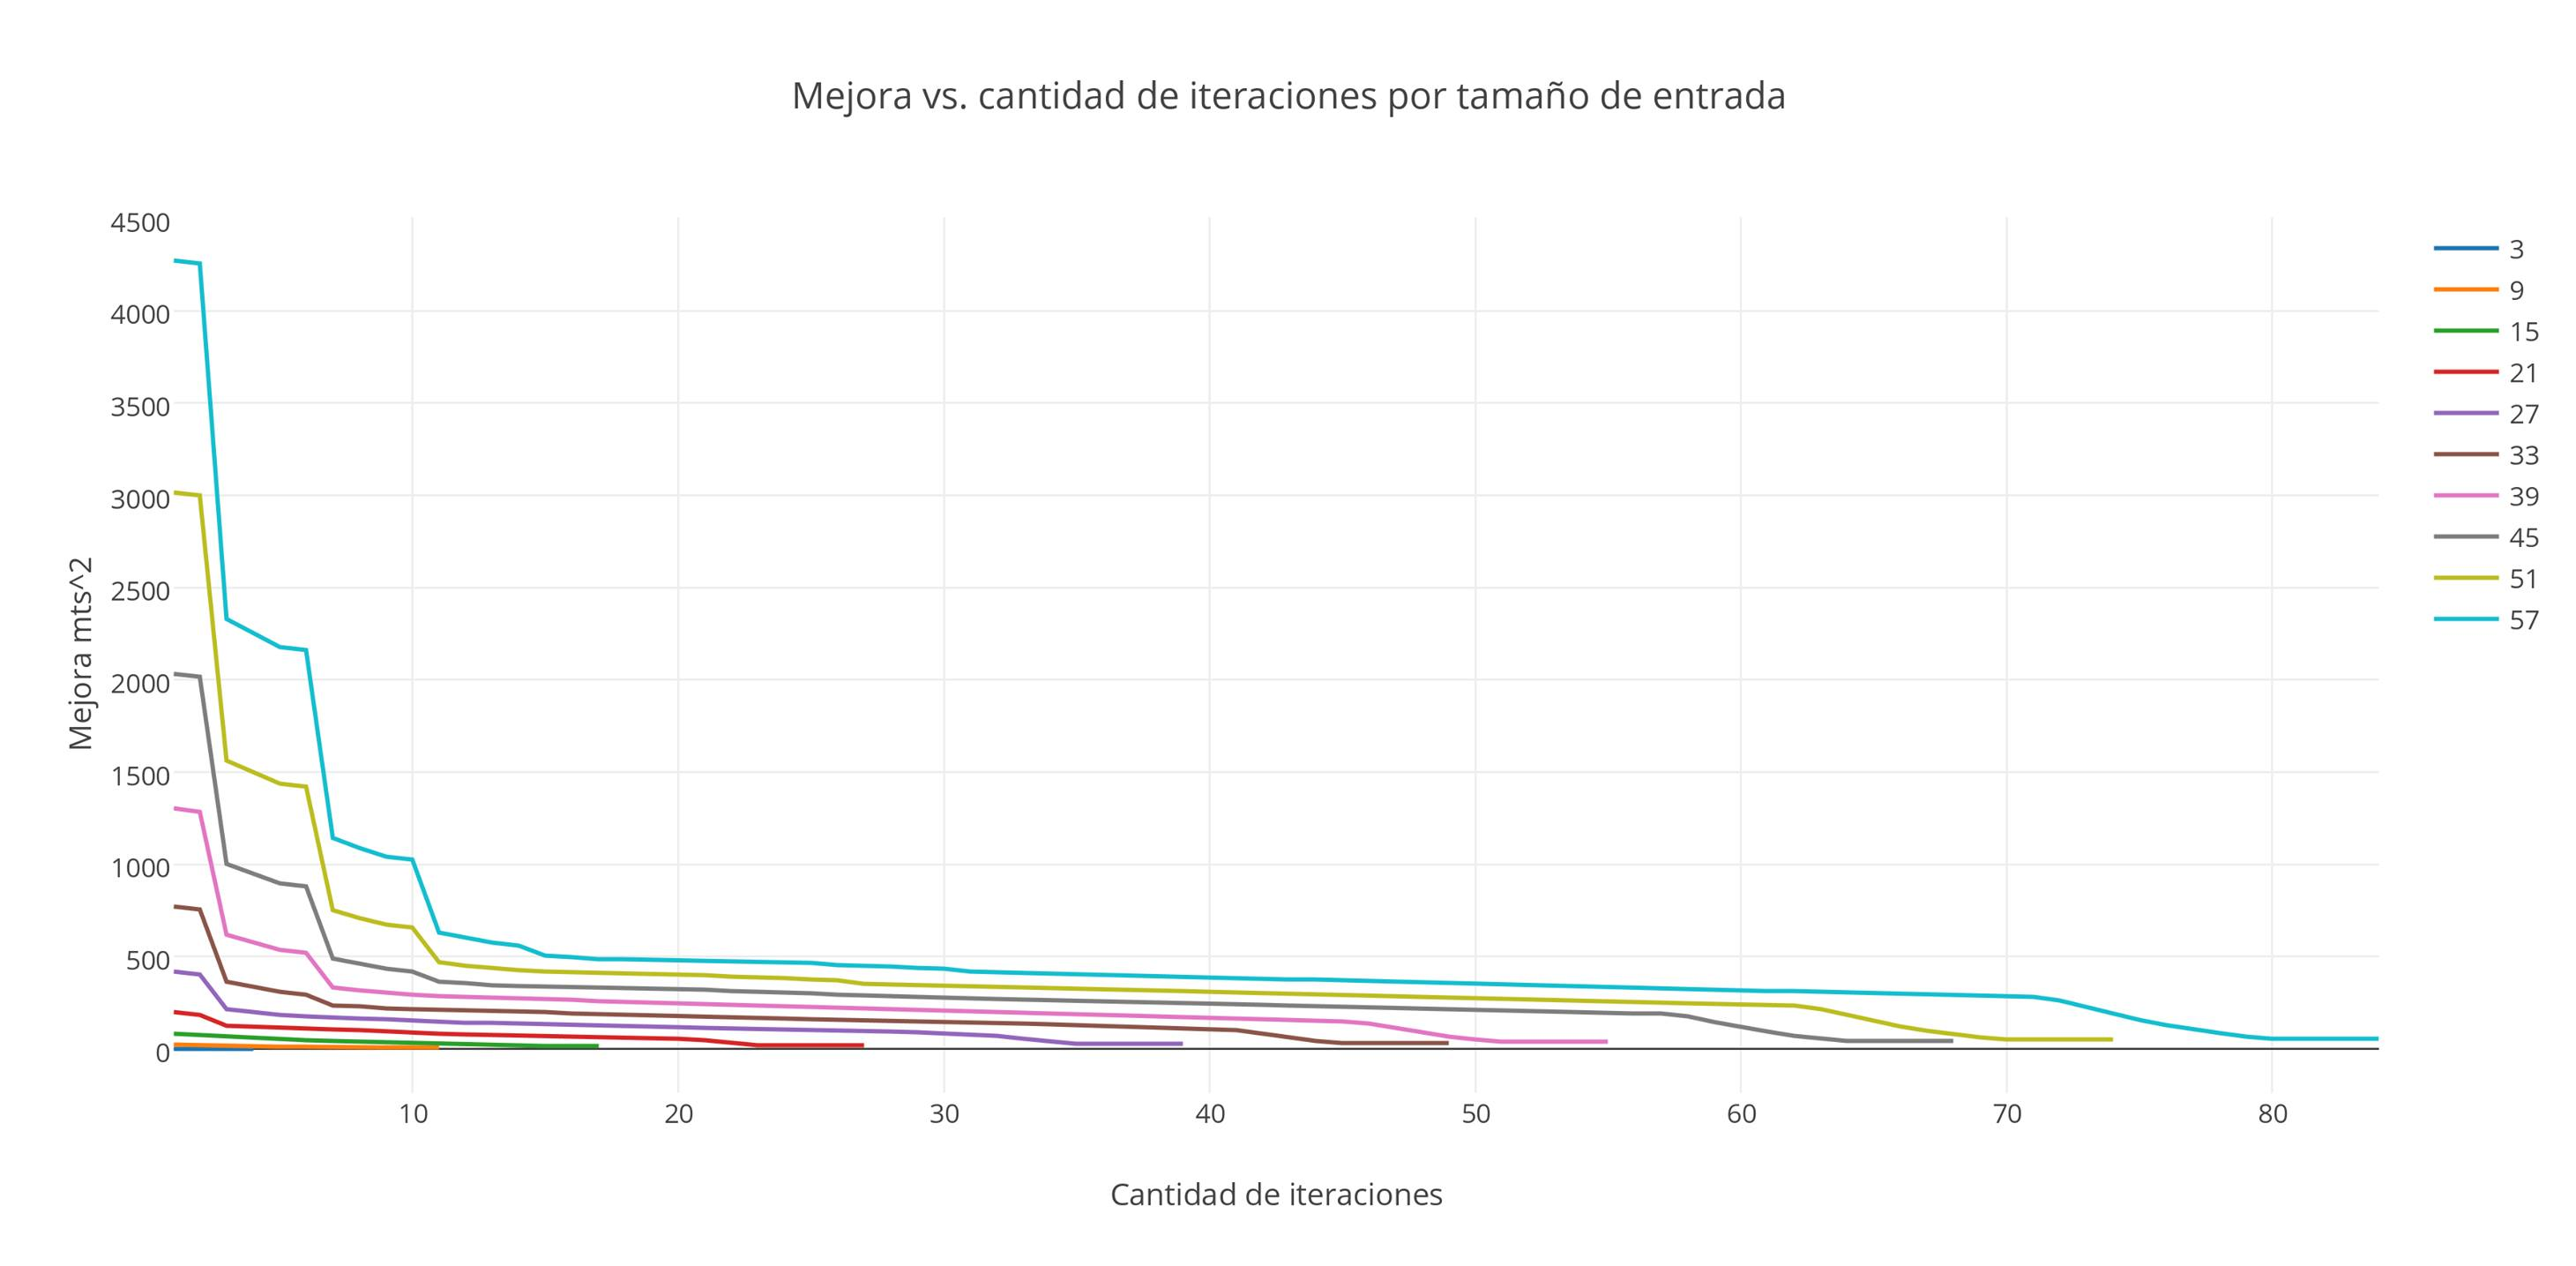
\includegraphics[scale=0.5]{./EJ4/mejora1.png}\\
 {            \textit{Gráfico \ 4.12 - Tabu 2-OPT vs Tabu 3-OPT sobre Familia 6}}
  \end{center}
  \vspace*{0.3cm}
  
  \vspace*{0.3cm} \vspace*{0.3cm}
  \begin{center}
 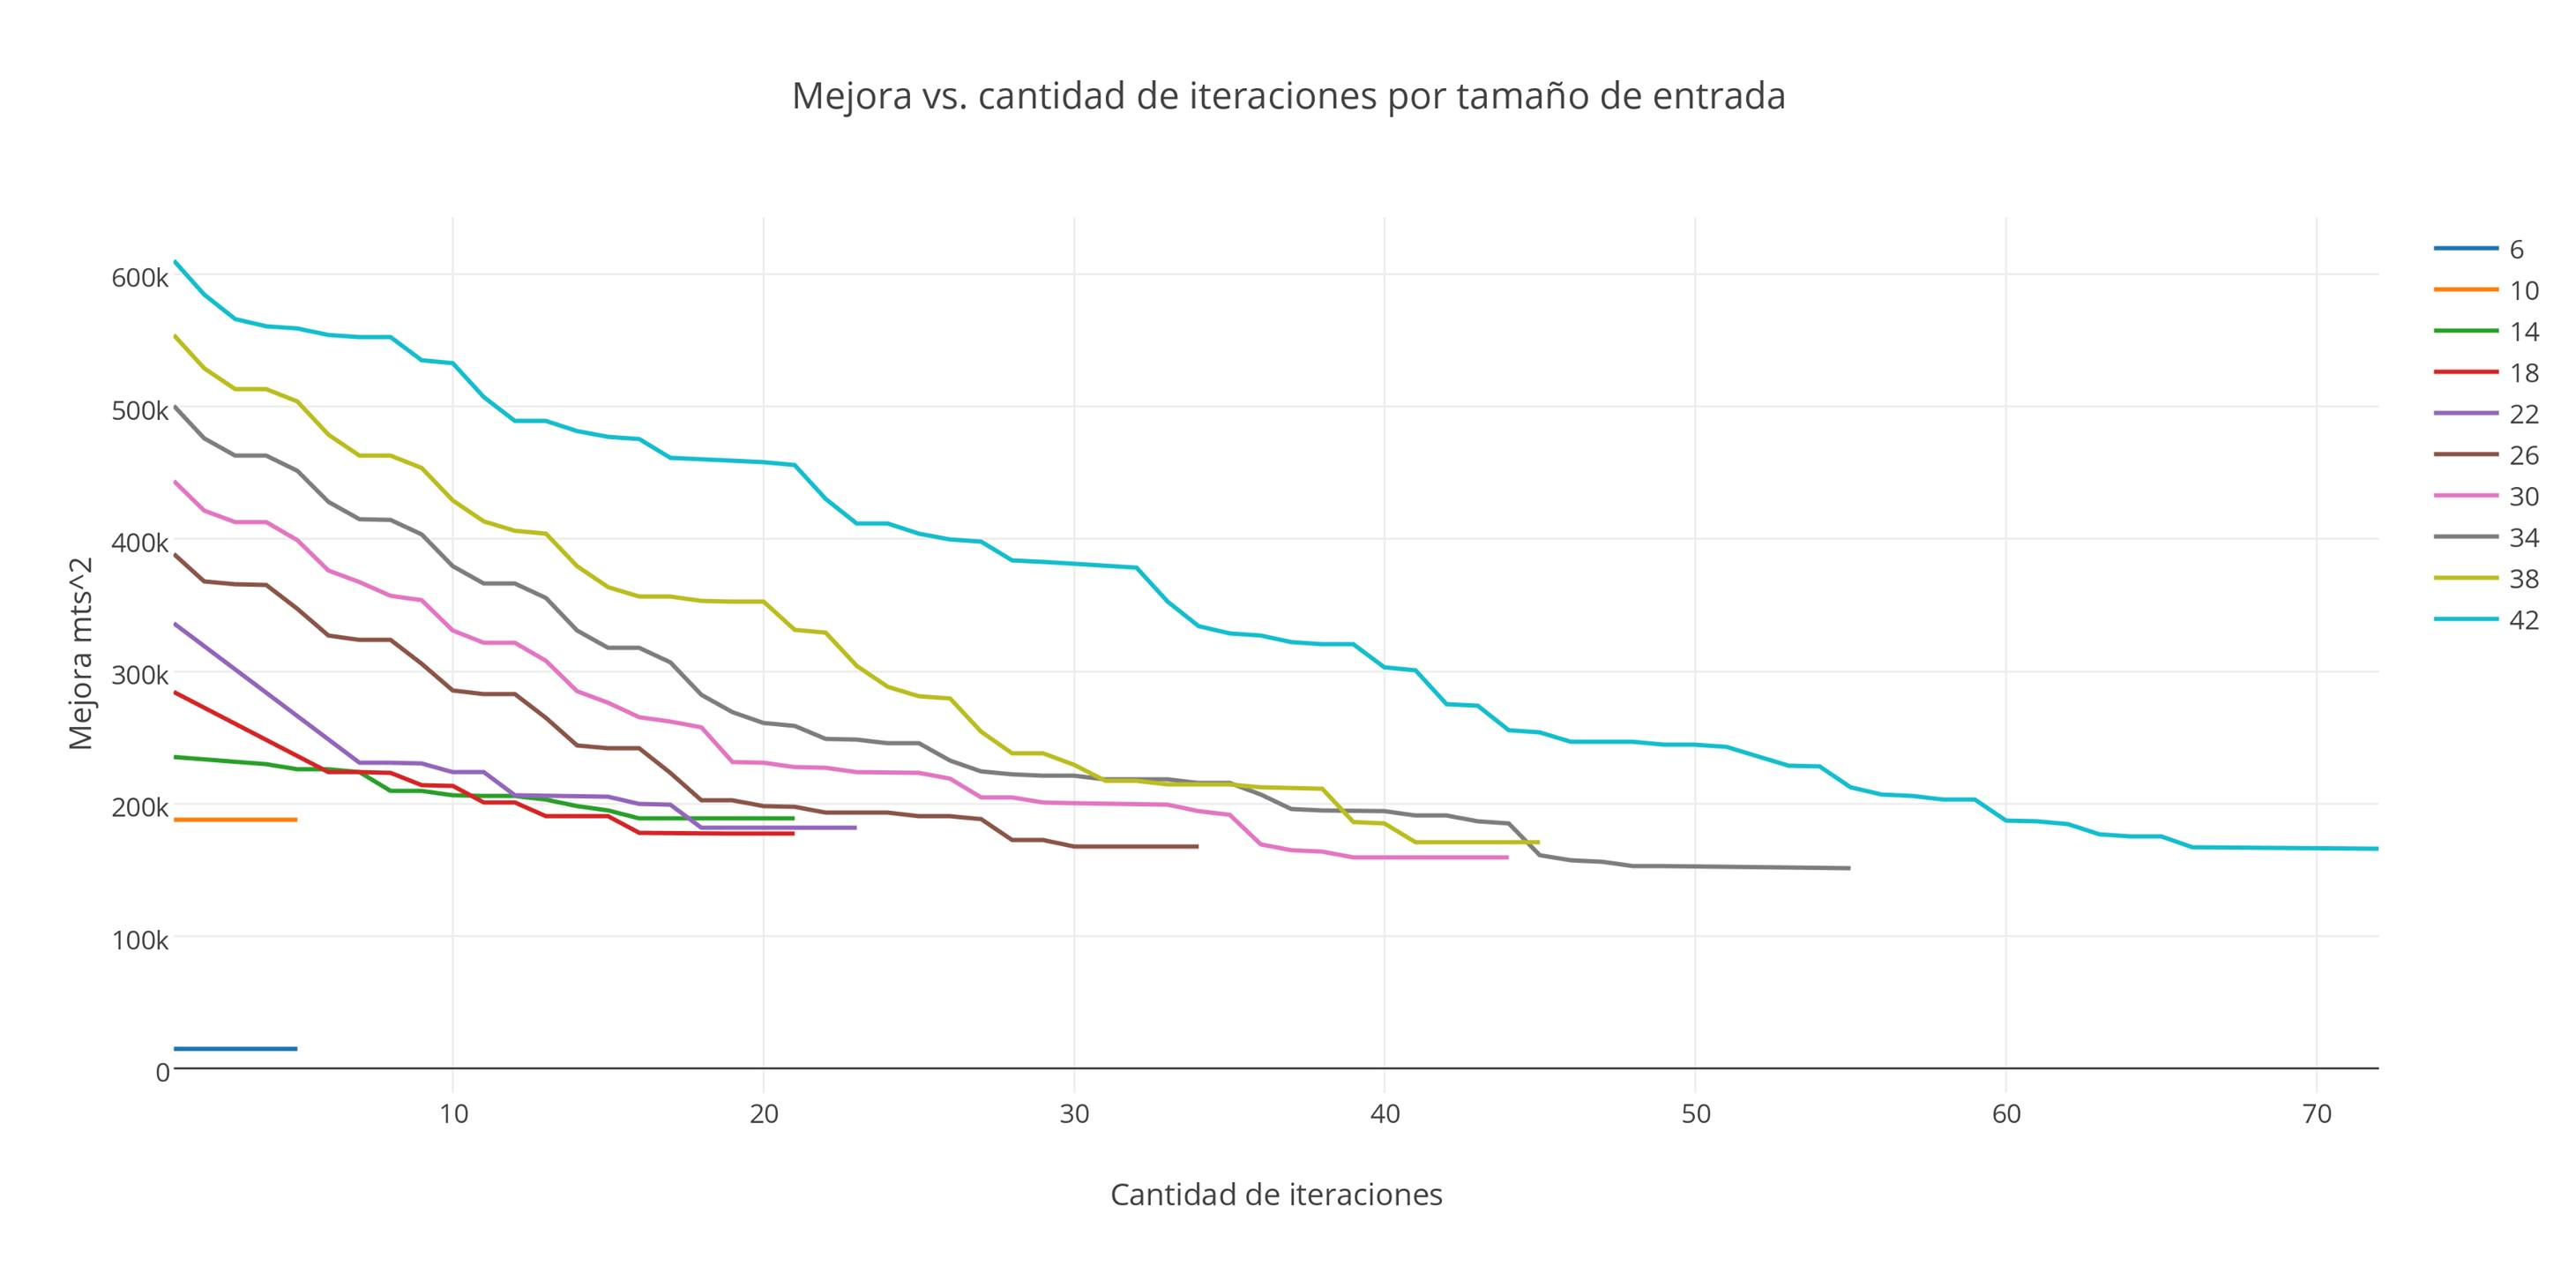
\includegraphics[scale=0.5]{./EJ4/mejora2.png}\\
 {            \textit{Gráfico \ 4.12 - Tabu 2-OPT vs Tabu 3-OPT sobre Familia 6}}
  \end{center}
  \vspace*{0.3cm}
  
--> OBTENER CONCLUSIONES GENERALES: PORQUE SIRVE? CUANDO CONVIENE ? CUANDO NO ? 
  


\newpage
\section{Ejercicio 5} 
\subsection{Enunciado del problema}
Una vez elegidos los mejores valores de configuración para cada heurística implementada (si fue
posible), realizar una experimentación sobre un conjunto nuevo de instancias para observar
la performance de los métodos comparando nuevamente la calidad de las soluciones obtenidas y los
tiempos de ejecución en función del tamaño de entrada. Para los casos que sea posible, comparar
también los resultados del algoritmo exacto implementado. Presentar todos los resultados obtenidos
mediante gráficos adecuados y discutir al respecto de los mismos.
\subsection{Experimientos y conclusiones}
\subsubsection[2.5]{Test}
En esta sección se compararon las distintas heuristicas implementadas en el trabajo. Por un lado, la heuristica golosa y por otro la heuristica de busqueda local.\\
Dada la naturaleza del problema, no existe un único factor a analizar como en trabajos anteriores en los que solo interesaba el tiempo de corrida. Sino que también, al ser un problema de optimización, entra en juego la calidad de las soluciones. \\

\subsection{Calidad de solución}
Primero analizaremos la calidad de las soluciones obtenidas por las heuristicas. Para realizar este analisis se implementó un generador de grafos aleatorios y en base a estos se corrieron los distintos algoritmos. \\
Estos experimentos se dividieron en dos etapas, uno que intenta medir la calidad de soluciones en grafos donde resulta posible su coloreo total y otro que toma en cuenta cualquier tipo de grafo.\\

Para medir la calidad de soluciones, consideramos el porcentaje de aristas sin conflictos (con ambos extremos pintados y de distinto color) sobre el total de aristas del grafo.

\subsubsection{Grafos coloreables}

Para realizar este experimento, se utilizó el generador de grafos aleatorios y se filtro a cada uno por los que el algoritmo del ejercicio 2 indicaba que eran coloreables. \\

Debido a la lentitud de este metodo, no se obtuvo un conjunto de grafos muy grande. \\

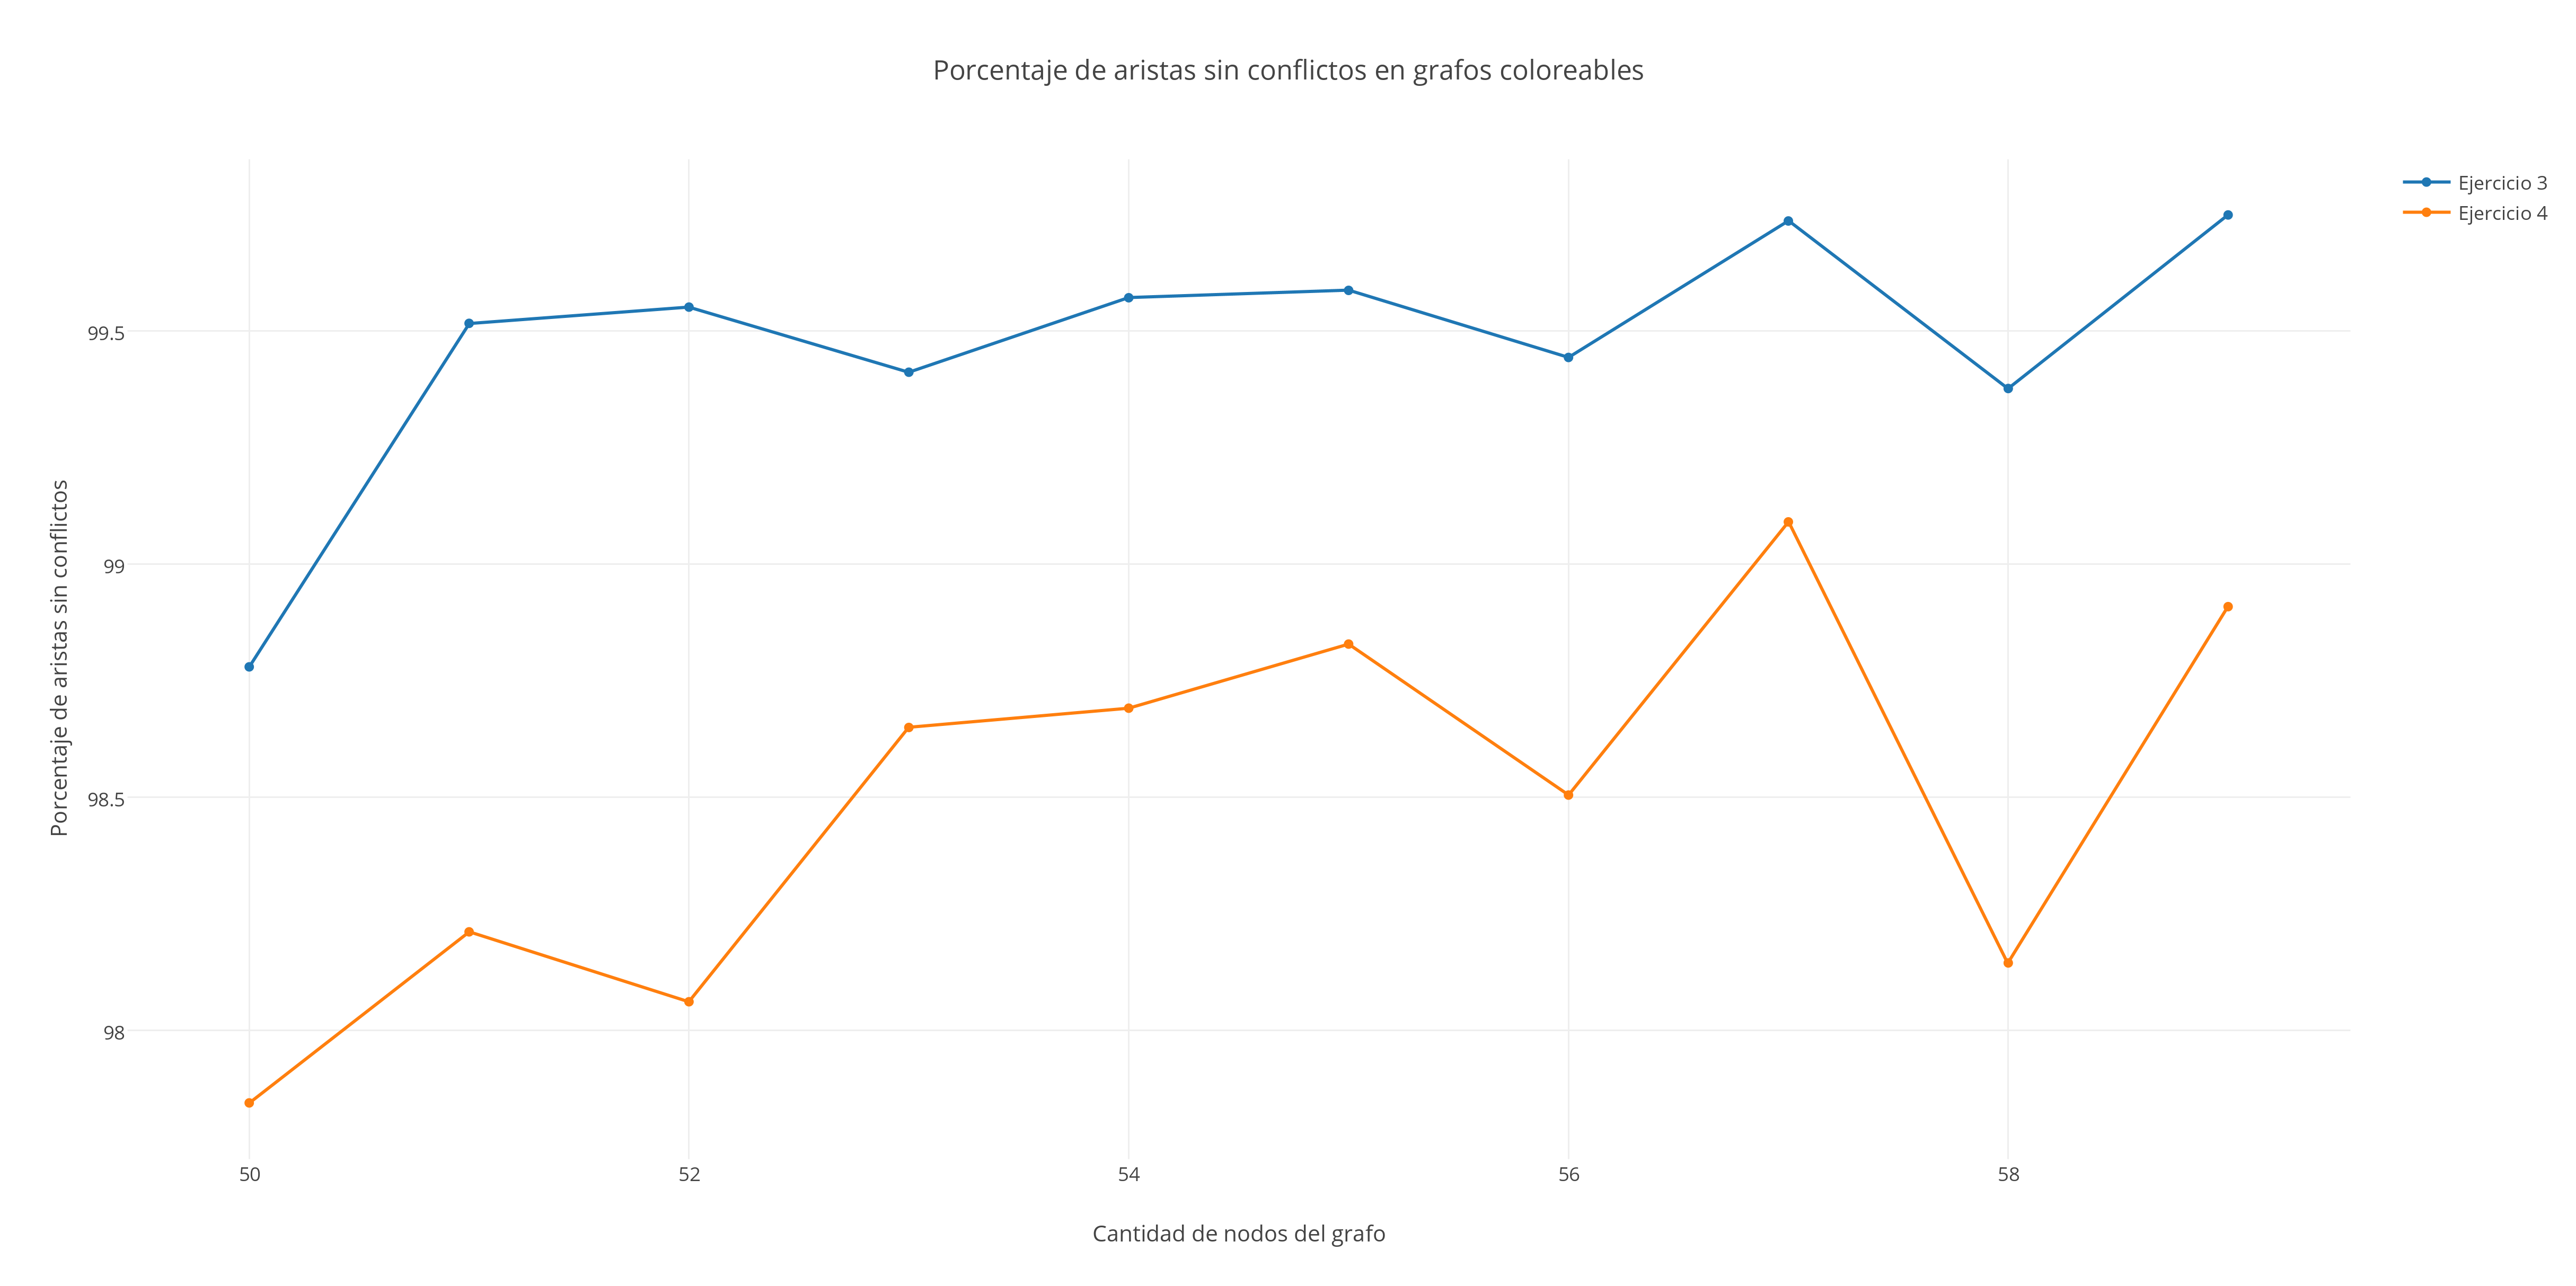
\includegraphics[scale=0.45]{./imagenes5/coloreables.png}
 	{}

En el gráfico anterior se puede notar, que si bien la heuristica del ejercicio 3 presenta soluciones mas cercanas para este conjunto de grafos, ambas están muy cercanas a la solución optima.


\subsubsection{Grafos no necesariamente coloreables}

En estos experimentos, tomamos grafos aleatorios variando tamaño y cantidad de colores. Se comparó la calidad de las soluciones provistas por los dos algoritmos.\\

En el siguiente experimento se corrió a los dos algoritmos con grafos de distinto tamaño, pero con 2 colores en total.
\includegraphics[scale=0.35]{./imagenes5/conf2.png}

Curiosamente, las calidades de solución son las mismas para los dos algoritmos. Lo que nos muestra que los algoritmos se comportan de manera muy similar para este caso. (Queda pendiente la demostración de este interesante hecho)\\
Esto nos lleva a la pregunta si se mantendrá esta similitud para los demás casos. Por lo tanto, aumentamos la cantidad de colores a 3, y aumentamos el rango de tamaño en los experimentos. \\

\includegraphics[scale=0.45]{./imagenes5/conf3.png}

Como podemos notar, las calidades ya empiezan a distinguirse entre los distintos algoritmos. Este caso da como ganador a la heuristica de busqueda local. \\

Realizamos un experimento más variando la cantidad de colores, pero siempre manteniendolos constante. La cantidad de colores elegidos fue de 10.\\

\includegraphics[scale=0.45]{./imagenes5/conf10.png}

Si bien con tamaños de grafo mas pequeños la heuristica golosa supera en calidad a la de busqueda local en calidad, luego de un aumento en el tamaño del grafo esta diferencia se revierte en favor del algoritmo del ejercicio 4. \\

Un dato interesante que no nos queda claro su por qué es el hecho de que en todos los experimentos con cantidad de colores fija $C$ pero con tamaño de grafo variable, la calidad se termina acercando al $100- \frac{100}{C}$ porciento. Por ejemplo, con $C=2$ estuvo alrededor del $50\%$, con $C=3$ alrededor del $66\%$, con $C=10$ alrededor del $90\%$. \\

Finalmente, decidimos probar con casos en los que la cantidad de colores aumenta linealmente con la cantidad de nodos del grafo. (Cada 4 vertices hay un nuevo color) \\

\includegraphics[scale=0.45]{./imagenes5/confv4.png}

Podemos notar al gráfico con saltos en los multiplos de cuatro, y esto es debido de que en esos casos los ejemplos pasan a tener un color más entre las opciones, por lo que el problema pasa a ser "más fácil" en general. \\
Esta comparación también da por ganadora a la heuristica de busqueda local. \\ \\

Resumiendo, pudimos notar en estos experimentos, que si bien en el analisis de calidad con grafos coloreables la heuristica del ejericicio 3 superó en calidad a la del 4, en los demás, esta última resultó ganadora. Creemos que los resultados del primer experimento se debieron a la poca cantidad de grafos analizados para analisis. \\

\subsection{Performance de solución}

En secciones anteriores las complejidades de cada algoritmo ya fueron estudiadas, y por lo tanto, se espera que los tiempos del algoritmo del ejercicio 3 sean notablemente menores que los del ejercicio 4.\\

En el siguiente gráfico se pueden comparar los tiempos de corrida para grafos de 2 colores en total.

\includegraphics[scale=0.45]{./imagenes5/t2.png}

Los tiempos resultan muy parecidos, ya que el hecho de que haya pocos colores en total hace que no sea notorio el factor $C$ que tiene la complejidad del algoritmo del ejercicio 4. Por lo tanto, decidimos aumentar el la cantidad de colores, esta vez a $5$.

\includegraphics[scale=0.45]{./imagenes5/t5.png}

Y ahora la diferencia de tiempos resulta notoria, como habiamos conjeturado al principio de esta sección. \\


\subsection{Conclusión de comparaciónes}
Conluímos con que no hay un claro ganador entre los algoritmos, ya que ambos presentan un intercambio entre performance y calidad. \\
Por lo tanto, que algoritmo es mejor dependerá de nuestras necesidades, es decir, de nuestro contexto de uso. Por ejemplo, si nos interesan soluciones con la mayor calidad posible podemos optar por la implementación del ejercicio 4. Por el contrario, si lo que nos interesa es la velocidad, podremos optar por la implementacion del ejercicio 3. \\
Para este tipo de comparaciones, siempre se debe responder preguntas como ¿Qué tanta calidad se necesita? ¿Cuánta performance se puede perder? ¿Los casos que me interesan analisar resultan muy beneficiosos para el primer algoritmo o no hay mucha diferencia?










\end{document}

